\documentclass[11pt, a4paper]{article} % , draft
\usepackage[utf8]{inputenc}

\usepackage{enumitem} % customiçe item dots etc
\usepackage{textgreek} % obv
\usepackage{physics} % for easy derivative notation
\usepackage{amsmath}
\usepackage{amsthm} %theorems
\usepackage{amssymb}
\usepackage{mathtools} % for matrices with blocks inside
\usepackage[scr=boondoxo]{mathalfa}
\usepackage{pst-node}%
\usepackage{mathrsfs}
\DeclareMathAlphabet{\mathpzc}{OT1}{pzc}{m}{it}

\newcommand{\mc}{\multicolumn{1}{c}}
\newcommand{\R}{\mathbb{R}} % command for real R
\newcommand{\Holo}{\mathcal{H}}
\newcommand{\M}{\mathcal{M}}
\newcommand{\C}{\mathbb{C}}
\newcommand{\N}{\mathbb{N}}
\newcommand{\z}{\mathpzc{s}}
\newcommand{\p}{\mathpzc{r}}
\newcommand{\s}{\mathbb{S}}
\newcommand{\W}{\mathbb{W}}
\newcommand{\U}{\mathscr{U}}
\newcommand{\Lg}{\mathscr{L}}
\newcommand{\x}{\mathcal{X}}

\usepackage{csquotes}
\MakeOuterQuote{"}
\setlength{\parskip}{0.3 cm}

\usepackage{fancyhdr}

%\usepackage{nath} % authomatic parenthesis stuff
%\delimgrowth=1
\usepackage[left=2cm, right=2cm, top=2.1cm, bottom=2.1cm]{geometry} % set custom margins
\usepackage{graphicx} % to insert figures
\usepackage{grffile}
\graphicspath{{Figures/}} % define the figure folder path
\usepackage{subcaption} % for multiple figures at once each with a caption
\usepackage{multirow} %multirow in tables

\usepackage{caption}
\captionsetup[figure]{font=footnotesize} %adjust caption size
\captionsetup[table]{font=footnotesize} %adjust caption size

\usepackage{booktabs} % for pretty tabs in tables
\usepackage{siunitx} % Required for alignment
\captionsetup{labelfont=bf} % bold face captations

\usepackage{hyperref} % makes every reference a hyperlink
\hypersetup{
    colorlinks=true,
    linkcolor=violet,
    filecolor=[rgb]{0.69, 0.19, 0.38},      
    urlcolor=[rgb]{0.0, 0.81, 0.82},
    citecolor=[rgb]{0.69, 0.19, 0.38}
}

\usepackage{epigraph} % for quotations in teh begginig
\setlength\epigraphwidth{8cm}
\setlength\epigraphrule{0pt}
\usepackage{etoolbox}
\makeatletter
\patchcmd{\epigraph}{\@epitext{#1}}{\itshape\@epitext{#1}}{}{}
\renewcommand{\qedsymbol}{o.\textepsilon.\textdelta}

\newtheorem{prop}{Proposition} %so I can use propositions
\newtheorem{cor}{Corollary} %so I can use corollaries
\newtheorem{defi}{Definition} %so I can use corollaries

\makeatother % all this is for the epigraph
\usepackage{tocloft}

\usepackage{imakeidx} % make index

\makeindex[columns=3, title=Alphabetical Index, intoc]

%\title{\vspace{-2.5cm} {\bf Can we make the Exponential scaling in Time\\ be Linear in Time if Parallelized Exponentially? \\ {\em - Part 2 -}} \vspace{-0.4cm}  }
\title{\vspace{-2cm} {\bf Quantum Dynamics  with\\ Waves and Trajectories}\\{\small by {\em Xabier Oyanguren Asua}}\vspace{-0.8cm}}
\date{\vspace{-11ex}}
\let\clipbox\relax
\usepackage{adjustbox}
\newcolumntype{?}{!{\vrule width 1.5pt}}
\usepackage{abstract}
\setlength{\absleftindent}{0mm}
\setlength{\absrightindent}{0mm}

\usepackage{tcolorbox}
\DeclareRobustCommand{\mybox}[2][gray!10]{%
\begin{tcolorbox}[   %% Adjust the following parameters at will.
        left=0.2cm,
        right=0.2cm,
        top=0.15cm,
        bottom=0.15cm,
        colback=#1,
        colframe=#1,
        width=\dimexpr\textwidth\relax, 
        enlarge left by=0mm,
        boxsep=5pt,
        arc=0pt,outer arc=0pt,
        ]
        #2
\end{tcolorbox}
}

\usepackage{anyfontsize}
\newenvironment{kapituloBerria}[1][]
  {\clearpage           % we want a new page          %% I commented this
   \thispagestyle{empty}% no header and footer
   \vspace*{\stretch{2}}% some space at the top
   \raggedleft          % flush to the right margin
   {\textbf{{\fontsize{60}{40}\selectfont \hspace{+9.5cm}#1\newline \newline}}}
   \bf
   \fontsize{30}{20}\selectfont
  }
  {\par % end the paragraph
   \vspace{\stretch{3}} % space at bottom is three times that at the top
   \clearpage           % finish off the page
  }

\usepackage{listings}
\usepackage{xcolor}
\lstset{language=C++,
                basicstyle=\ttfamily,
                keywordstyle=\color{blue}\ttfamily,
                stringstyle=\color{red}\ttfamily,
                commentstyle=\color{green}\ttfamily,
                morecomment=[l][\color{magenta}]{\#}
    backgroundcolor=\color{black!5}, % set backgroundcolor
    basicstyle=\footnotesize,% basic font setting
}

\begin{document}

\clearpage
%% temporary titles
% command to provide stretchy vertical space in proportion
\newcommand\nbvspace[1][3]{\vspace*{\stretch{#1}}}
% allow some slack to avoid under/overfull boxes
\newcommand\nbstretchyspace{\spaceskip0.5em plus 0.25em minus 0.25em}
% To improve spacing on titlepages
\newcommand{\nbtitlestretch}{\spaceskip0.6em}
\pagestyle{empty}
\begin{center}
\bfseries
\nbvspace[1]
\Huge
{\nbtitlestretch\huge
QUANTUM DYNAMICS WITH \\ WAVES AND TRAJECTORIES}

\nbvspace[1]
\normalsize

WHAT IF THE OBSERVED QUANTUM\\
SYSTEM IS A FLUID ELEMENT?\\
\nbvspace[1]
A Guide to the Equations \\Governing Quantum Dynamics

\nbvspace[1]
\small BY\\
\Large Xabier Oyanguren Asua\\[0.5em]
%\footnotesize Can we really foresee the future of the Universe?"\\


\nbvspace[6]


\includegraphics[width=2.5in]{UAB.png}
\normalsize
\vspace{-0.5cm}
%\small Thesis Directors: \\
%\nbvspace[0.2]
%\large Jordi Mompart Penina \\
%Xavier Oriols Pladevall\\
%\nbvspace[1]

%Universitat Autònoma de Barcelona\\
\large
%DEGREE FINAL DISSERTATION \\
\small
%Bachelor's degree in Nanoscience and Nanotechnology \\
\small
$\ $September 2021 
\nbvspace[1]
\end{center}
\newpage
\null
\clearpage

\maketitle
\pagenumbering{gobble}
\setlength{\cftbeforesecskip}{0.4cm}
\setlength{\cftbeforesubsecskip}{0.4cm}
\setlength{\cftbeforesubsubsecskip}{0.25cm}

\tableofcontents
\clearpage
\pagenumbering{arabic}
\setcounter{page}{-2}
\vspace{-0.3 cm}
%\section{The Objective}
%It is well known that the time dependent Schrödinger Equation (TDSE) that predicts the dynamics of a quantum system is a problem that scales exponentially both in space and in time for increasing dimensionality of the problem. This becomes very obvious when interpreting the wave-funtion in terms of an ensemble of tangentially interacting trajectories of the system. That is, quantum mechanical systems (experiments) depend on all their possible realizations in a way that all the possible trajectories of the system interact repulsively among them due to the quantum potential first described by David Bohm. This means that it is equivalent to think on the wavefunction of the system as an ensemble of an infinitely dense set of exactly equivalent systems forming a fluid where each copy of the system cannot cross the trajectory of any other at the same time (they cannot occupy the same point in configuration space-time) and they still have a repelling force pushing the fluid towards the most homogenenous distribution possibel given the manifold described by the potential energy term. 
%
%This clearly shows that it is impossible to evolve a single one of these trajectories without knowing the whole ensemble. This is the so called Quanutm Wholeness. This means that if we increase the dimensionality of the system, it is not enough to increase the computational complexity linearly. A single dimension more implies that in order to know about one single trajectory we now need to know as many trajectories as we needed for the previous dimensionality multiplied by all the possible positions in a new axis. The number of trajectories we would need to simultaneously compute in order to be able to even compute them (and by the way reconstruct the wave-funtion in tyheir vecinity) increases exponentially. However, it is still not clear that there is no method that could allow us evolve self-consistently in parallel at each time step enough trajectories, such that their evolution is linear in time for increasing number of dimensions (even if it scales exponentially in parallel threads that communicate at each time step).
%
%That is, the question is, can we find a method that allows us to compute a single time step that has a fixed cost (perhaps with soem overheads for parallel communiocation) that transfers the expoenntial complexity to the parallelization? That is, it is clear, that if we try to sequentially compute the necessary number of trajectories to advance a central trajectory, we need exponentially more surrounding trajetcories, thus in the single thread's time we would require exponentially more time. Then, even if we are given as many parallel computation threads as we want, we are not able to compute all the trajectories, because they are not independent and they do influence each other. Still, if we allow a cross talk between them every time step, we could achieve an evolution for them that does not increase the complexity in sequential time (unless for the overhead). This cross talk would account for the qwuantum potential propagation. Osea esto es fundamentalemte posible si consiguiese encontrar cual es el pair-wise quantum potential discreto, que al hacer al infinito tiende a la funcion de onda continua. Si fuese asi con una integracion del sistema de edos infinito (pero cada eq simple) en paralelo actualizando los potenciales para cada uno podrias conseguir resolver cualquier problema quantum many body problem si tuvieses suficientes threads paralellos (uno por cada trayectoria evolucionada). HAbria claramente el problema del cross talk, que seria cada vez mas complicada pero bueno, en si seria eso.
%
%Alternativamente, en vez de intentar hacer que todas las trayectorias sean por igual ecuaciones d eNewton, queiza podrias intentar darle un empujon y evolucionar fks de onda condicionadas y una trayectoria por cada conjunto. Ya que cada CWF es 1D y eso es muy facil de resolver. Si fueses capaz de aproximar la full fk de onda con estas slices en cada dimension mejor que usando las trajs en si pues mejor. Ze en si cada CWF es un ensemble de trayectorias, pero de las cuales en principio solo uan (la central) es en cada tiempo la misma. Osea la pregunta es realmente el qtm wholeness necesita trayectorias que estan super lejos? Claro, la cuestion es que no seras capaz de obtener con un solo set de cwf-s en cdad dimension (una trayectoria) evolucionada al mismo timepo el self-impulso dado por las trayectorias que lo rodean. Aka una sola cwf evolucionada en paralelo no funkiona. En todo caso muchas cwf-s evolucionadas tangentemente si, como las trayectorias. Pero esto por supuesto acabaria siendo un ensemble method tipo quantum trajectory method. 
%
%
%Osea la cuestion es que la velocidad e duna trayectoria de Bohm solo depende de la derivad de sus CWF-s en cada timepo! de las direcciones ortonormales (ze claro, el campo de velocidades es la derivada parcial (en las dirs cartesianas de la accion) y el qtm potential solo depende de la derivada parcial en las dirs cartesianas de la "densidad" local!). Entonces, dado un t, dada la fk onda completa, sacas condicioanndo las CWF. Ahora de las CWF tu puedes computar a donde se mueve la traj de Bohm en el sigueinte teimpo. Ahora la pregunta es, puedes si supieses toda la traj evolucionar un tiempo la CWF? Si pudieses ya estaria reuslto el problema many body. Pero la resuesta es que las ecuaciones que rigen las CWF dependen de la full wavefunction al parecer!
%
%Disclaimer, all the present work will be made for 3 dims but is clearly generalizable to N.
\pagestyle{empty}

\section*{Abstract}
Quantum dynamics using waves is not new, but neither is using just trajectories, as can be found in the 2006 handbook by Wyatt \cite{Wyatt}. What is still to be explored is the full potentiality of mixing both things in the time evolution of a quantum system. That would mean treating a subsystem as a fluid with its constituent trajectories and treating the rest of the system in terms of a wavefunction. We can readily find many references in the literature to the so called conditional wavefunctions \cite{conditional1}, \cite{conditional2}, but there is no proper guide towards them. How can one situate them in the landscape of the main quantum dynamics equations?



\section*{Objectives}\vspace{-0.2cm}
The present document is a review of the panorama we face when talking about quantum dynamics involving trajectories and waves in a same standing. It is intended to be an essay that situates the conditional function approach in a pedagogical narrative, in terms of degrees of freedom treated in the Lagrangian or the Eulerian frames. Its main objective is to provide a global view of the panorama that could light possible paths for the development of new algorithms that could exemplify the potentiality of the mixed wave-trajectory approach.


\section*{Guideline}\vspace{-0.2cm}

It is highly recommended to have the index of contents beside while reading the document in order to have a schematic view of the description, since at some points the details can get a bit technical and the reader may loose the perspective.

The document is divided in two blocks.

 In the first block, we will first give a brief qualitative insight to the terms employed throughout the work, concerning the different interpretations of quantum mechanics and concepts in fluid mechanics. After that, we will present a heuristic view of the possible approaches in terms of degrees of freedom, that one can take when dealing with a quantum system. Then, we will have a quick tour over the different computational methods with which we can attack each of them. 

In the second block, we will dig into the quantitative equations of quantum dynamics within each degree of freedom treatment. We will divide this exposition in three main sections. We will first visit the fully Eulerian picture, which is the typical pure wave view. We will then explore the fully Lagrangian picture, which is the one manifesting the quantum system in terms of trajectories in all of its glory. Finally, we will arrive to the mixed description, where we will have part of the system described in the Eulerian and part in the Lagrangian frame. It is there where the conditional function burden will be finally exposed. In the three of them, the same equations will be reviewed but in their corresponding approaches. That is, the section (I.b) will be the equivalent to the sections (II.b) and (III.b) but each one will describe them through their own perspective, as we will see. It is this why it is convenient to have the schematic index at hand at all moment.

\newpage

\begin{kapituloBerria}[Part A]
Drafting the Panorama
\end{kapituloBerria}
\newpage
\null
\clearpage

\pagestyle{fancy}

\fancyhead[R]{\em On the Employed Notation and Vocabulary}
\section*{On the Employed Notation and Vocabulary}
\addcontentsline{toc}{section}{Part A: Drafting the Panorama}
\addcontentsline{toc}{subsubsection}{On the Employed Notation and Vocabulary}

Throughout the document concepts of the Orthodox, Bohmian, Hydrodynamic and Tangent Universe interpretations will be employed altogether in order to give names to the mathematical tools we will employ. Let us thus, have a brief brainstorm on them to set things in place.

Given a system whose possible ontological configurations can be labelled by a set of $N$ coordinates or degrees of freedom\footnote{They could be $N$ one dimensional particles, $N/3$ three dimensional particles etc.} $(x_1, ...,x_N)\equiv \vec{x}$, which can take continuous values in a certain subset of $\R^N$, say $\Omega_t\subseteq \R^N$, we call the set of possible values of $\vec{x}$, the {\bf configuration-space} of the system. We introduce an additional labelling axis, called time, $t$, together with the concept of dynamics, which is the evolution in time of the quantitative properties of the points in configuration-space. Note that the subset of $\R^N$ that we consider may vary continuously in time, thus the subindex $t$ in $\Omega_t\subseteq \R^N$. In order to describe a set of quantitative properties of this continuous contingent extension in configuration-space and time, we shall use a set of scalar functions that map points in configuration-space $\vec{x}$ and time $t$ to numbers $\{f_k(\vec{x},t)\}_k$. These properties shall be called the {\bf state variables} or {\bf properties} of the system, and should be enough as to be able to predict the time evolution of themselves. 

There are two ways in which we could understand these state variables, described by $f_k(\vec{x},t)$. On the one hand, they could be interpreted as inherent properties of configuration-space points $\vec{x}$. Such that each, scalar value for a point $\vec{x}$ in configuration-space is an "intrinsic" time dependent property of that point. Alternatively, we could understand these scalar functions as properties of a fluid, an underlying movement of points filling the configuration-space $\Omega_t$, where each point carries with it {\em its} values of the quantitative properties. Among the properties of those points moving in configuration-space, as an additional state variable, there is their position $\vec{x}\in\Omega_t$. This means that according to this fluid vision, we will observe a certain value for a state variable at a configuration-space point $\vec{x}$, not because the value is telling us something inherent about that point $\vec{x}$, but because it describes a property of the {\em fluid element} that happens to be crossing that point at that time.

Before talking about anything else, we see thus a necessity to formalize this continuum of uncountably infinite point like "particles" moving in configuration-space. An $\R^N$ point is a possible static configuration of the whole system, assuming that a possible system is always observed in space as point-like in all its degrees of freedom. This turns out to be our case, since we always observe fundamental particles to be point-like in in space. As we will see later, if for example, $N$ are all the degrees of freedom in the Universe, a point in $\R^N$ is a possible position for all the $3D$ particles in it (where there would be $N/3$ particles). Thus, a moving point in $\R^N$ or an element of that fluid, could be seen as a possible Universe, and its time evolution as the discrete Universe  we observe to be. The trajectory of one of these points would mean tracking the change of the positions of all the $3D$ particles in the Universe. We could call it, the trajectory of a possible Universe. In general, let us call these constituent elements or moving points of the $\R^N$ fluid, {\bf fluid elements}, {\bf possible experiments} or {\bf possible Universes}. Since we are talking about an uncountably infinite amount of moving points in configuration-space, but we assume that each fluid element occupies a {\em unique} point like position $\vec{x}$ at each time, we could label each of these fluid elements by their position at a reference time $t_0$ (which we shall call the initial time). We will then label for all times, the fluid element that is in the position $\vec{\xi}\in\Omega_0\subseteq \R^N$ at time $t=t_0$, simply as, the fluid element $\vec{\xi}$. Since we assume that these elements never cross each other (never collide and occupy the same configuration-space point at the same time) and they move to the nearby configurations crossing all the intermediate ones, we will assume there is a continuous function $\vec{x}(\vec{\xi},t)\equiv \vec{x}^{\, \xi}(t)$ that tells us where in $\Omega_t$ each fluid element $\vec{\xi}\in\Omega_0$ is at each time $t$.\footnote{Note that we call $\Omega_0$ the subset of $\R^N$ where we consider there are fluid elements at the reference time $t=t_0$. } This is what we call the {\bf trajectory} of the $\vec{\xi}$-th fluid element. Now, since each fluid element $\vec{\xi}$ has a continuously varying different position in $\Omega_t$ at each time, we see that the function $\vec{x}(\vec{\xi},t)$ must have an inverse function $\vec{\xi}(\vec{x},t)\equiv \vec{x}^{\, -1}(\vec{\xi},t)$, telling us which is the label of the fluid element crossing the configuration-space point $\vec{x}$ in time $t$. This inverse must be continuous as well, since the transformation $\vec{x}(\vec{\xi},t)$ is required to be continuous in all its variables. Thus, we are asking that $\Omega_t$ is homeomorphic to $\Omega_0$ at all times. For now, this seems to be just a convenience, but we will find it is a necessity within quantum mechanics. Since we will achieve the description of the time evolution of the positions of the fluid elements through the integration of a continuous velocity field, by the Picard-Lindelöf theorem, we will have that the transformation $\vec{x}(\vec{\xi},t)$ must be a spatial homeomorphism. What is more, it will need to be differentiable, meaning it must be a diffeomorphism.

\begin{figure}[h!]
  \centering
    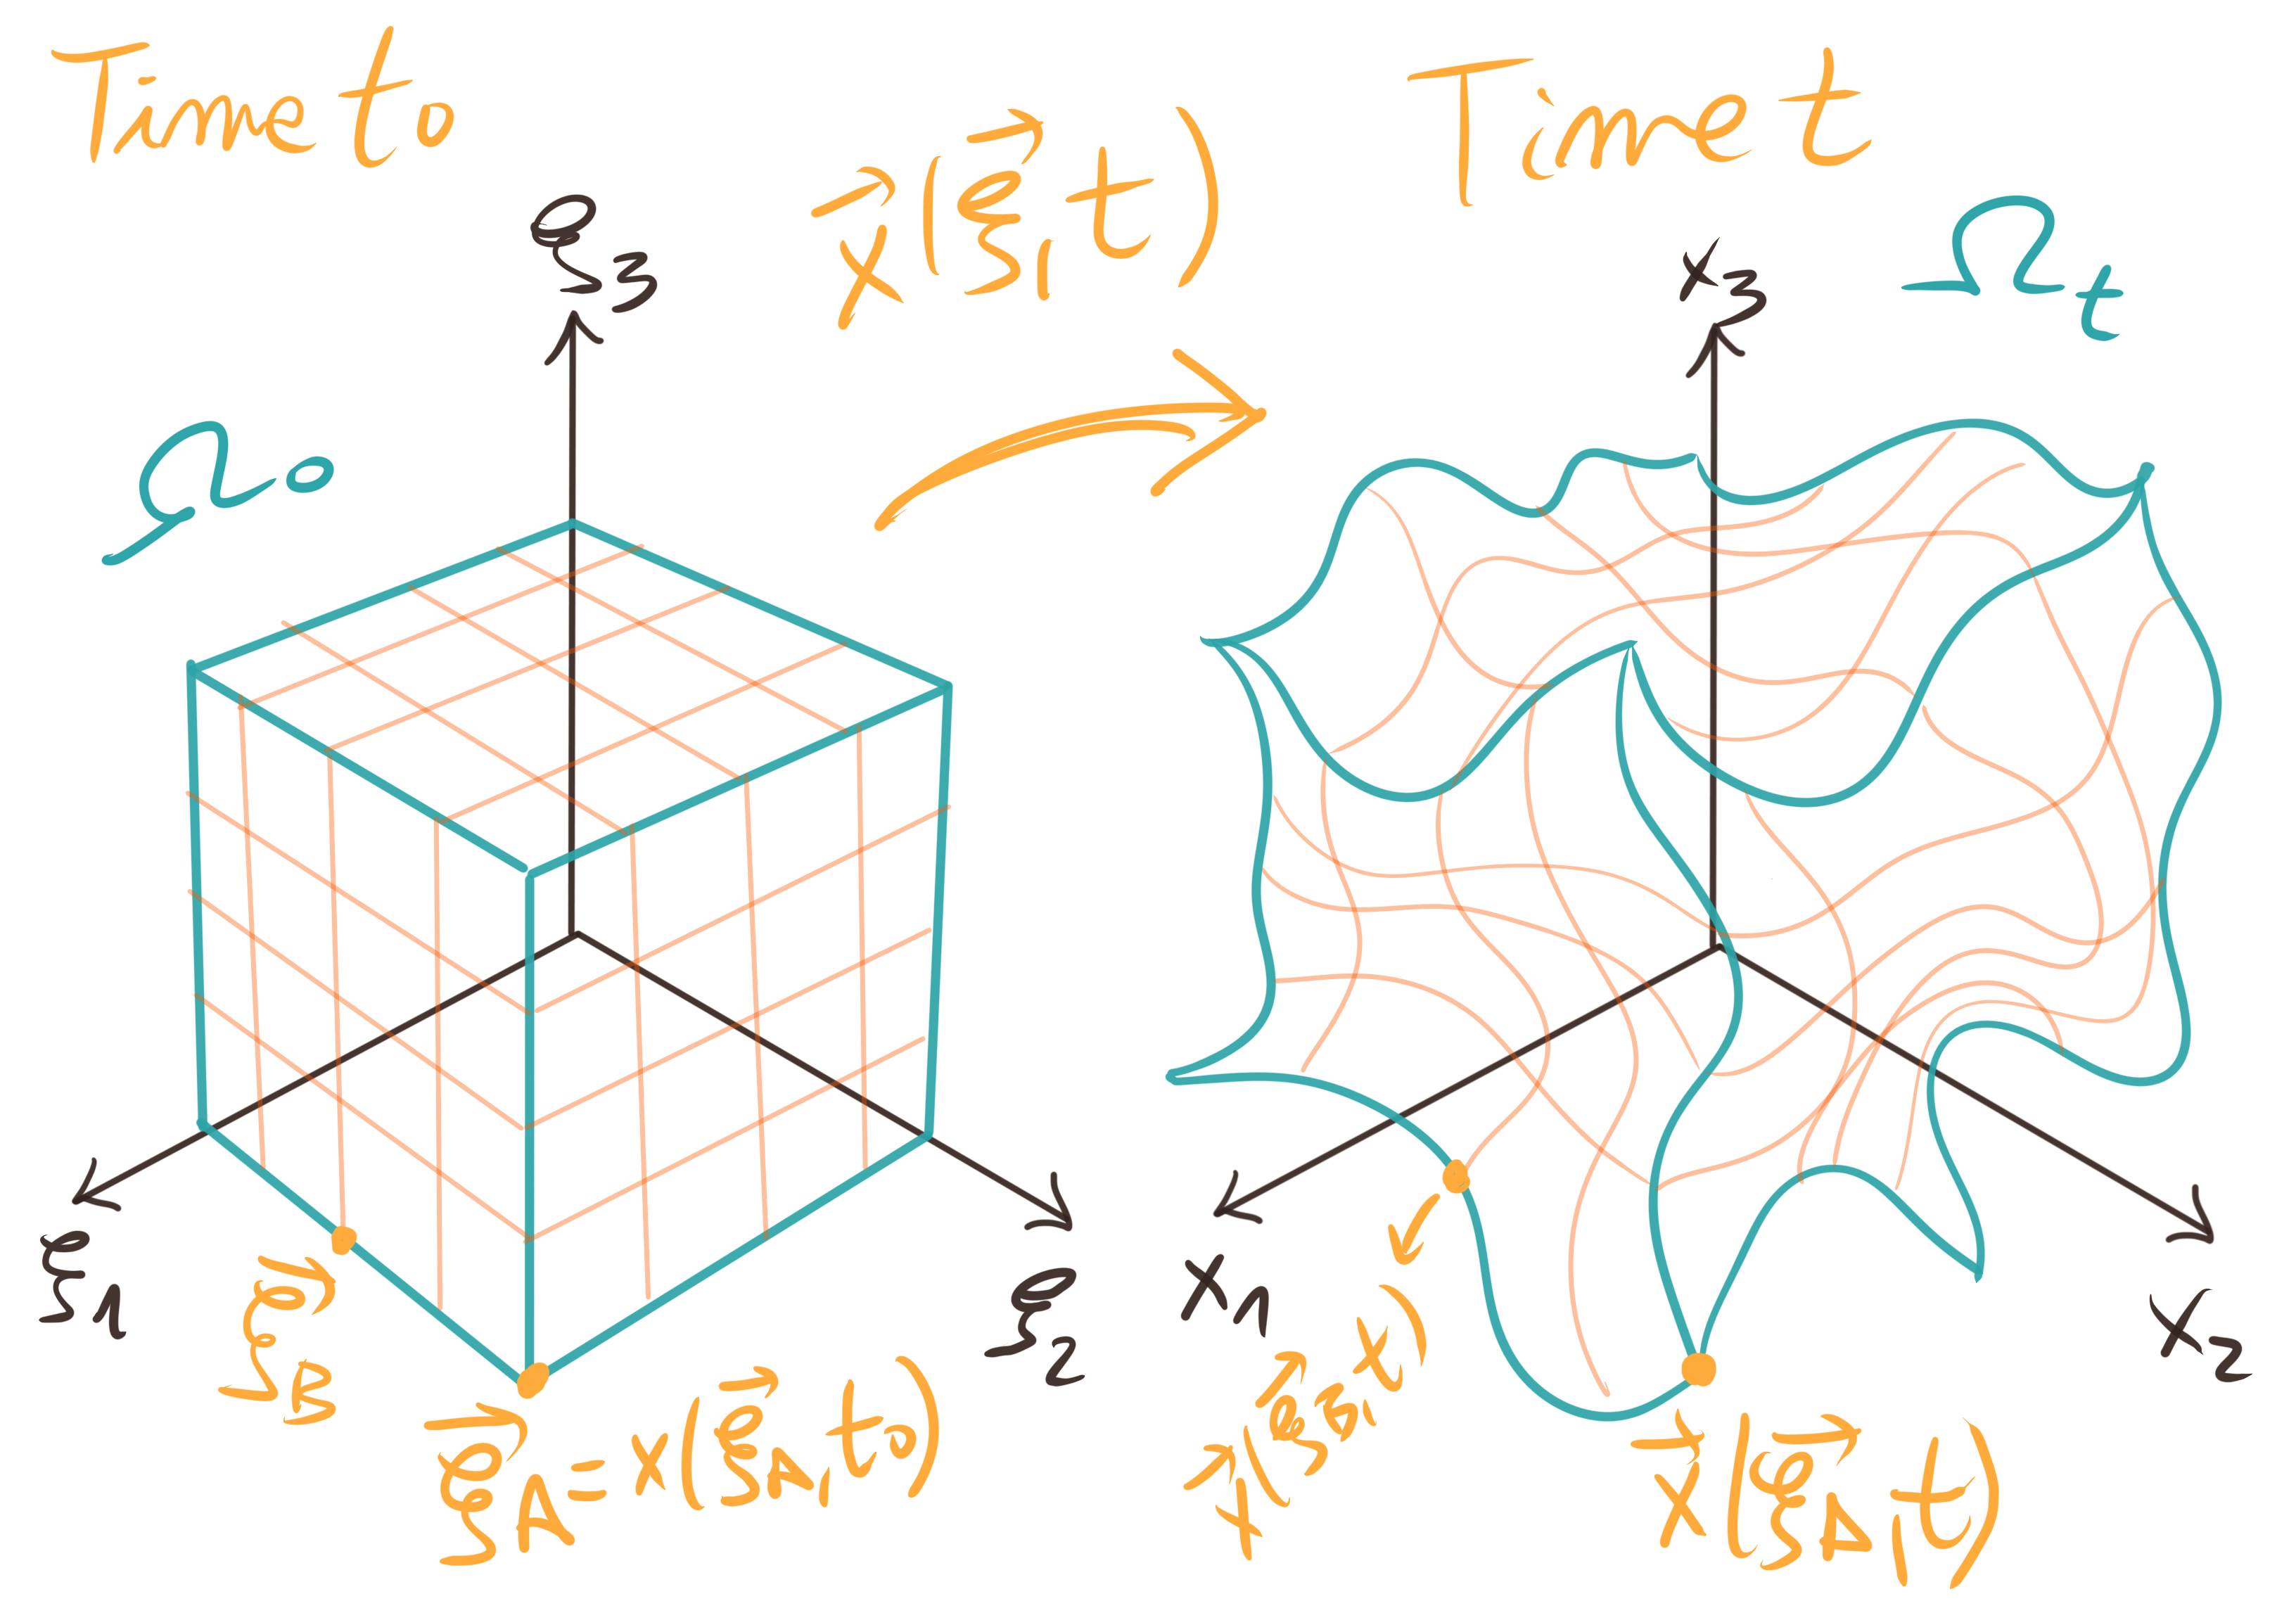
\includegraphics[width=0.57\linewidth]{1deforma.png}
  \caption{Depiction of the $N=3$ case of a diffeomorphism representing the trajectory ensemble of a fluid following the notation presented in the text. \vspace{-0.2cm}}
  \label{fig:deform}
\end{figure}

We can now realize that we will be able to describe a state variable of the system, both by reference to a specific configuration-space position $\vec{x}$ at a certain time $t$ or by reference to a specific fluid element (or possible Universe or experiment) $\vec{\xi}$ at a certain time. These will be respectively the Eulerian and the Lagrangian frames. 

In short, if for example, the configuration-space $\Omega_t$ represents the set of tuples of all the positions in 3D space of each particle in the Universe, then each point $\vec{x}\in\Omega_t\subseteq \R^N$ will represent a particular macroscopically observable configuration of the Universe. Tracking all the fluid elements in $\Omega_t\subseteq\R^N$ and the fields $f_k(\vec{x},t)$ would then mean that we can track the time evolution of each particular initial configuration of the Universe $\vec{\xi}$ in time, along with the properties of the quantitative scalars perceived from each of them $f_k(\vec{x}(\vec{\xi},t),t)$ (Lagrangian frame). Alternatively, we could see the value of the properties at each time from a particular preferred Universe configuration $\vec{x}$, as $f(\vec{x},t)$ (Eulerian). The interest on the particular case of $N$ being all the degrees of freedom in the Universe is that in reality, for a true description of natural phenomena, we require taking into account the interactions and restrictions between all the possible degrees of freedom. Thus, taking as our system, the biggest possible system, is roughly an imperative for interpreting a fundamental theory of nature.

In a nutshell, we define the {\bf Eulerian} frame of the system, as the description of the properties of the system as seen from each configuration-space point $\{f_k(\vec{x},t)\}_k$. For each $\vec{x}\in\Omega_t$, we will know the values of the state variables of the system. This view is compatible with both the non-fluid and the fluid interpretations. The {\bf Lagrangian} frame of the system on the other hand, will be knowing about the values of the state properties by knowing them as observed by each fluid element along their trajectories $f_k(\vec{x}(\vec{\xi},t),t)=f_k(\vec{\xi},t)$ (note the abuse of notation). 
 
As we will mathematically formalize in the following section, according to non-relativistic quantum mechanics, a single complex state variable, or equivalently, two real state variables, are enough for the full description of the time evolution of an isolated system (say, the whole Universe). This complex quantity is the so called {\bf wave-function}, which we will denote by $\psi$. The real fields are then its magnitude squared and its polar phase. These are the so called {\bf density}, $\rho$ (which can be interpreted as the density of fluid elements and will be responsible for the observable results at each time), and {\bf action} $S$ (the gradient of which in configuration-space yields the velocity field for the displacement of the fluid elements).

The wavefunction is the basic ontology within the {\bf Orthodox} interpretation of Quantum Mechanics. Here, each fluid element is just a mathematically valid tool for obtaining equations, but has no interpretative representation. Only the overall density and relative phases of the action field (velocity field variations) have physical significance. The density gives the probability density to find the system in each configuration-space point $\vec{x}$ at each time, while the relative action changes will be responsible for its wave-like interferences. This is the most pragmatic interpretation of the mathematical model, since it just provides an interpretation for the observable results, with all its corresponding interpretative paradoxes due to its philosophical vagueness. 

The {\bf Bohmian} interpretation understands the fluid elements driven by the velocity field given by the configuration-space gradient of the action $S$, to be the {\bf possible trajectories} of the system, the time evolution of possible observable experiments, from which only happens to exist one: the so called {\bf Bohmian trajectory} of the system. The rest of fluid elements composes the so called {\bf pilot wave}, that should be understood as an aura or wave driving the Bohmian trajectory, even if each fluid element mathematically composing the wave is also a possible Bohmian trajectory for another experiment. That is, the bundle of possible (but not simultaneously existing) Bohmian trajectories composing the pilot wave has no special significance. This pilot wave drives {\bf the} (single) existing Bohmian Universe (in $\R^N$), by a repulsive interaction in configuration space, just like a leaf in a current (in an $\R^N$ current), in a way that the Bohmian trajectory itself has a separate ontology from the pilot wave (just like the leaf and the water current). The possible trajectory that is said to exist is the one we observe when physically observing the quantum system, which happens to be a sample statistically obeying the probability density given by the density field {\bf of} the pilot wave. This is how Bohmian Mechanics ultimately matches orthodox predictions. It is because of that that in a Bohmian perspective, the fluid elements could also be seen as the time evolution of "possible experimental outcomes". But note that this means that possible experiments (that do not simultaneously occur) interfere between them, even if only one of them is truly existing (this is in the author's opinion the point that makes Bohmian still uncomfortable). That is, the rest of possible experiments that do not exist, which form the pilot wave, which turns out to be directly unobservable, influence what reality is. What is the nature of this pilot wave, its {\em arkhe}? No body seems to know it.

Finally, there is the {\bf Tangent Universe} interpretation, which understands that all of these fluid elements or Universes exist on a same ontologically contingent basis, as a swarm of possible Universes that interact repulsively whenever one of them approaches all of its degrees of freedom to another one (whenever two Universes become similar in all of their degrees), such that they always avoid crossing each other. Thus, instead of parallel Universes, which suggests that there is no influence between them, it is more convenient to call them, tangent Universes: they never cross, but they never stop to push each other. That is, each "possible experiment", each possible Bohmian trajectory composing the pilot wave, that interacts with the actually observed Bohmian trajectory, is here understood as a physically contingent Universe that physically "pushes" the one we happen to be in. We never see these other tangent Universes, and we always see a single point like trajectory of the whole system, that is, one definite position for each particle in the universe, because we, as observers, are trapped in one of these trajectories. Or have you ever experienced a superposition? Has there ever been any experiment finding that the electron is not point-like? The answer is no. And as fluid elements never cross, we will always be "trapped" in this Universal trajectory, and will only perceive the rest of "Universes" through the tangent force they exert on each degree of freedom of ours. Our lack of knowledge of the position of all the particles in the Universe, makes us thus, be in one of the possible Universes with equal probability, which means that our Universe will be a sample of the relative density they follow. Thus allowing the same predictions as Orthodox or Bohmian Mechanics. This interpretation gives the same material basis to both the density and the velocity field. No need for an unobservable pilot wave. Just like dark matter or dark energy, we feel a physical influence of them, their information is implicit on our Universe, they are necessary to predict its behaviour and the rules of its motion, but we cannot observe their origin directly. We can still measure clearly their contingent effect on every single quantum experiment we perform! How many years more are we ready to close our eyes in front of this?

There is finally a {\bf discrete} version of the last interpretation, suggesting that in fact, it is not necessary that these tangent Universes are infinitely uncountable. If we have a large enough amount of Universes only interacting between them through a repulsive force acting in proportion of their distance in configuration space, we can recover in the limit the quantum potential and quantum dynamics. This however, if the number of tangent Universes is not big enough, could result in different predictions to the quantum case. It is yet interesting to consider it for potential numerical methods!\vspace{-0.3cm}

\fancyhead[R]{\em On the Possible Approaches and Methods}

\section*{Approaches with Respect to the Degrees of Freedom}
\addcontentsline{toc}{subsubsection}{Approaches with Respect to the Degrees of Freedom}
\vspace{-0.2cm}

Let us list the main four approaches we can adopt in the context of quantum dynamics involving trajectories and wavefunctions. Approach I gives predominance to waves, while II gives it to trajectories. Approach III gives a weighted predominance to both, while IV forgets about continuous waves.
\vspace{-0.2cm}
\begin{enumerate}
\item[\bf ( I )] {\bf Mainly a Wave: } We could consider a fully wave-like picture, where the properties of the fields are intrinsic to configuration-space points, we just forget about the underlying fluid elements. This implies considering just the dynamics of an N+1 dimensional wavefunction in configuration-space $\psi(\vec{x},t)$. We will call this approach the {\bf Fully Eulerian Picture}. If we present trajectories in this description, these will only be computed {\em a posteriori} and will not be required to be known for the time evolution of the system. This approach is the typical one within Orthodox Quantum Mechanics (if only considering the wavefunction) and can be understood within Bohmian Mechanics (BM) or Tangent Universe Mechanics (TUM) (by considering also the {\em a posteriori} trajectories).


\item[\bf ( II )]{\bf Mainly Trajectories:} We could view the quantum system as a fluid of moving fluid elements in configuration-space. The values of the field will now be relevant at the positions of {\bf Lagrangian frame} trajectories $\{\vec{x}^{\, \xi}(t)\}_\xi$. These last will be computed {\em a priori} together with the other state variables perceived by the fluid elements. This is what we will call the {\bf Fully Lagrangian Picture}. This approach is easiest to be interpreted through TUM. It is also the most consistent one with BM even if there is no explicit pilot wave. BM would understand these elements as possible Bohmian trajectories (or as a granulation of the pilot wave).

\item[{\bf ( III )}]{\bf Waves and Trajectories in Equal footing: } We could consider a scheme where {\bf part} of the quantum system (the degrees $\vec{y}=(x_{m+1},...,x_N)$) is considered to be described by fluid elements in $\R^{N-m}$, in the Lagrangian-frame and {\bf part} of the system (the degrees $\vec{x}=(x_1,...,x_m)$) is a field in the Eulerian-frame. This will imply considering several waves $\{ f(\vec{x}, \vec{y}(\vec{\xi}_y,t), t) \}_{\vec{\xi}_y}$ which will describe the state variables in a Lagrangian frame for each fluid element $\vec{\xi}_y$ describing the $N-m$ axes $\vec{y}$, together with a description of the state properties in an {\bf Eulerian frame} for the other $m$ degrees $\vec{x}$. These are the so called {\bf conditional functions}. Note that we will need to compute the trajectories $\vec{y}(\vec{\xi}_y,t)$ that will describe the motion of the {\bf Lagrangian frame} elements {\em a priori}, together with the conditional waves. 
%It is a mixed approach between evolving a wave equation and evolving purely trajectory equations. If we wish to assign to it a preferred interpretation, possibly BM would be comfortable with this, since it would see the Eulerian degrees as the Pilot Wave itself. For this however, it would be necessary to define complementary conditional wavefunctions $\{ \psi(\vec{x}_a(\vec{\xi}_a,t), \vec{x}_b, t) \}_{\vec{\xi}_b}$, so as to get simultaneously, Bohmian trajectories (fully Lagrangian) and the pilot wave (which is acceptable in a fully Eulerian frame). Both trajectories and wavefunctions are "a priori".


\item[\bf ( IV ) ]{\bf Only Trajectories: } We could view the quantum system not as a continuum, not as a continuous distribution of $\R^N$ point like fluid elements, but instead as an ensemble of many discrete particles in $\R^N$ that feel a repulsive force among them acting on configuration-space. Except for this configuration-space interaction, the system would behave fully classically. In the limit of many discrete Universes, typical Quantum Mechanics predictions should be recovered. The density would then be computed as the agglomeration of trajectories employing a histogram or by computing the Jacobian of the system and the velocity field as a nearest neighbour average. Here the wavefunction would only be computed {\em a posteriori} if required and the trajectories would be the only {\em a priori} elements. This approach can be understood under the prism of the "Discrete Tangent Universe Interpretation".\vspace{-0.3cm}
\end{enumerate}
Very importantly, note that for all the interpretations all these approaches are mathematically equally valid. However, some interpretations consider some of the approaches as mere mathematical tools, useful for calculations but nothing else.
%But then why do we It is interesting to wonder however, why Orthodox physicists do not also consider other aspects of physics, like the concept of mass, or dark energy, or electrons themselves as "mere mathematical tools".


\section*{Panorama of the Methods We Can Study \vspace{-0.15cm}}
\addcontentsline{toc}{subsubsection}{Panorama of the Methods We Can Study}
Quantum Mechanics is well known for its many body problem, where the number of {\bf operations} needed to simulate its dynamics grows exponentially with the number of degrees of freedom $N$. This wall is unbreakable in terms of operations. However, we can rather deliver these operations in {\bf sequential time} or deliver them in {\bf parallel processes} that can share information, in order to make the problem faster in terms of effective sequential time. In particular, as we will prove in the last section, we can obtain a polynomial scaling in sequential time, at the cost of using exponentially more parallel processes\footnote{Assuming always that the overhead of the process messaging does not grow exponentially with dimensions $N$}. In this line, trajectory based methods are naturally parallelizable (even if we we will see some technical ways to parallelize fully Eulerian equations as well). The philosophical argument that weights the tread-off is that we cannot wait years for a computation, but we can always build bigger supercomputers with more parallel processors.

It turns out that there are some techniques that try to make the exponential {\bf operation} problem be polynomial, but those are based on rather applying approximations to the equations (the Hermitian approximation, density functional theory etc.) or on having {\em a priori} knowledge about the system (knowing the eigenstates of the Hamiltonian of the system, knowing the expected quantum correlations etc.)\footnote{Or both things at once, as we did in the Truncated Born-Huang Expansion of the tensor product of conditional wavefunctions for a particle in a channel.}. These methods are also useful, even if they are not really arbitrarily generalizable.

In the second block of the treatise, we will formalize the exact equations employed within each degree of freedom approach, and we will have the option to suggest numerical methods thereof. However, for an initial brainstorm, let us overfly now some of the main numerical methods employed within each approach:\vspace{-0.25cm}
\begin{enumerate}
\item[\bf ( I )] {\bf Mainly a Wave - Eulerian Picture}:\vspace{0.15cm}

To solve these equations, there are lots of fixed grid methods, ranging from using naive finite differences, Runge-Kutta Methods, to matrix methods like Crank Nicolson. Also, expressing the wavefunction in a certain function basis and then evolving the coefficients could be considered a kind of method (we will see this one in detail). Then there are the Spectral and Pseudo-Spectral methods based on changing the Schrödinger Equation to other representations, like the momentum representation, involving the Fourier transform, related conceptually with the basis representation methods. 

Except in the case where we know analytically the Hamiltonian eigenstates or some sub-system Hamiltonian eigenstates, in general the approach to the Eulerian wavefunction allows no escape from the exponential sequential-time barrier and are methods hard to be parallelized. Even though we will see that understanding the system in terms of fluid elements will allow a parallelizable framework also within a fixed grid.\vspace{0.2cm}

\item [\bf ( II )] {\bf Mainly Trajectories - Lagrangian Picture :}\vspace{0.15cm}

This approach basically consists on a dynamical grid of points or fluid elements that move according to some velocity field. Each fluid element will know the evaluation of the relevant fields, like the polar phase and magnitude of the wavefunction, along the trajectory it traces. Thus, fluid elements encode the field at the points they are on. The ensemble of these values over several trajectories can serve as feedback for each fluid element to individually know the next values and positions they will take, as we will see in a moment. It is known in general as the family of Quantum Trajectory Methods (QTM), which was boosted by {\em Wyatt et al.} at the beginning of this century. A very good reference, in which the present work was partially inspired is his handbook \cite{Wyatt}. According to the law of motion for the fluid elements that we choose, QTM-s can be classified in two ways:
\begin{enumerate}
\item An option is to define the velocity field driving the fluid elements of the dynamical grid according to the configuration-spatial gradient of the action. If done so, the trajectories are driven by the probability density flow lines, so they shape Bohmian trajectories. This assumption makes some dynamical equations and correlation terms simpler. However, Bohmian trajectories avoid nodal regions of the pilot wave, so the grid of points can get under-sampled or over-sampled for different regions in an uncontrolled manner. At the same time this can be an interesting property, since the mesh as a whole will roughly follow the densest parts of the wavefunction. The second problem that Bohmian trajectories have (as many others will) is that the grid of elements gets very unstructured, which can be problematic to compute the spatial gradient of the action among other essential terms.

\item Using adaptive grids. Choosing the velocity field of the fluid elements so as to trace custom trajectories designed by the user. For instance it can be chosen such that the fluid elements preserve certain monitor functions in each path, so the grid distorts itself to become denser around high fluctuation regions. We will dig into these methods in detail. Many additional methods, like adding a viscosity or friction term, are very useful here in order to avoid unstabilizing the evolution due to spiky fluctuations of the quantum potential.
\end{enumerate}

Both kinds of choices for the velocity field have the problem that in order to compute the time evolution of the properties carried by the fluid elements, configuration-spatial derivatives $\pdv{}{x_k}$ are required along the trajectories. This means that the single value of the field each element drives is not enough to know its spatial variation. This problem, sometimes called the {\em Quantum Wholeness}, can in general be faced in two different ways: by evolving an ensemble of fluid elements that can serve as a moving grid to reconstruct the full function and then allow numerical derivatives, or rather by treating the derivatives as additional fields of interest over the trajectories. In general, the first ones of these, allow us to compute the derivatives in one of the following two ways:

\begin{enumerate}
\item Using the values of the field over the ensemble of trajectories as an unstructured grid, one can fit a linear sum of analytic functions (by maximum likelihood, least squares, gradient descent etc.), at each locality of each trajectory. This sum can be symbolically derivated and integrated. Alternatively a K nearest-neighbour interpolation could also be useful, avoiding parametric function fitting. Both of these have an additional complexity that must be taken into account.

\item Employing the chain rule, one can convert the derivatives with respect to configuration-space $\vec{x}$ variables to derivatives with respect to label space $\vec{\xi}$. If we choose the initial grid to be a regular Cartesian grid, then these last derivatives will be in a regular grid at all times and will be simple to compute using finite differences. To do this change however, we will require the knowledge of the Jacobian matrix for the transformation $\vec{x}(\vec{\xi},t)$ and its determinants. The time evolution will still get more costly than what initially looked like.

\end{enumerate}
All of these methods are in general very parallelizable if we allow messaging between the processes in each time step, but non of them is clearly a miracle. Finally, if we treat the derivatives themselves as well, as state variables to be computed along the trajectories, one can avoid computing a whole ensemble of fluid elements (with its consequences) by, among others:
\begin{enumerate}
\item Finding dynamical equations for the derivatives of the required field quantities, one can evolve the derivatives themselves along each trajectory, allowing the {\bf individual} fluid element evolution. The cost of this will be that the number of partial differential equations in play will be increased, actually, as we will see, an infinite number of them will appear. To face this, truncating the series at some point will be necessary, with all its consequences.

\item By deeply knowing the problem and employing {\em ad hoc} shapes for the derivatives of the fields (for the quantum potential, the correlation terms etc.), one can get by without the need for an ensemble. However, this way lacks generalizability and one could argue that we are somewhat unfairly, externally introducing part of the solution.\vspace{0.2cm}
\end{enumerate}


\item [\bf ( III )] {\bf Waves and Trajectories in Equal Footing - Part Lagrangian, Part Eulerian Picture:}\vspace{0.15cm}

We will have that part of the problem to be solved (the Eulerian one) is similar to case (I) and part (the Lagrangian one) similar to case (II). Therefore, we will have the freedom to use one of the methods mentioned in (I) to solve the partial differential equations of the Eulerian parts, mixed with the approaches used for (III) in order to account for derivatives in the axes where we only consider Lagrangian elements. We will have control over the degree at which we place more or less weight into one or the other problem. Thus, we could arrive at a compromise that has all the main advantages of both methods but ideally less of their problems.

Following the discussion in the previous section, the trajectories could be chosen to be Bohmian, if they follow the fluid flow, but could also be chosen to be otherwise, in order to achieve an adaptive grid that explores the regions of configuration space we are most interested on.

Following the same ideas, we will be able to solve the derivative problem in several ways:
\begin{enumerate}
\item Evolve many of these conditional functions with coupled trajectories in order to be able to rebuild the full function and then get the derivatives in $x_k$ for the Lagrangian axes. This could be done by fitting functions or using nearest neighbour approaches. Exponentially less conditional functions will be required to be computed for increasing dimensionality of their Eulerian part, since the reconstruction will require less conditional functions. However, they will also be each time more complex to compute. Conversely, exponentially more conditional functions will be needed for decreasing dimensionality of their Eulerian degrees, but each one will be simpler to be evolved.

\item Convert the derivatives with respect to undesired Eulerian degrees $x_k$ into derivatives with respect to label space or Lagrangian degrees $\xi_j$. If we choose the Lagrangian elements to shape a regular grid at the initial time, then we will always have the option to compute derivatives in a regular grid using the information of the different conditional functions. We will also need to evolve several conditional functions for this.

\item Generate dynamical equations of the derivatives in the Lagrangian axes, that can be evolved as well along the trajectories. This would allow to evolve a single conditional wavefunction "exactly". It turns out that an infinite chain of equations will emerge here too.

\item Knowing the problem, approximate the problematic terms at the theoretical level, {\em ad hoc}, for the given system.
\end{enumerate}

Clearly, approach III is the generalization of approach I and II, those last being the two extreme cases. Condition it all or condition nothing.\vspace{0.2cm}

\item [\bf ( IV )] {\bf Only Trajectories:}\vspace{0.15cm}

In this approach, we can choose a large enough number of configuration space trajectories and evolve them using classical mechanics, introducing the necessary repulsive potential between all the trajectories so as to replicate Quantum Dynamics. If the number is large enough, then the theory will be a good enough approximation of continuum Quantum Mechanics. The point is that there will be no need for the trajectories to "carry" any information about any wave. They are ontologically sufficient to describe quantum phenomena. If we need information of quantum nature, we will just see the wavefunction (the density and action) as the ensemble limit of the trajectories. From the moving histogram we can fit a density function, or else use the Jacobian determinant of the trajectory mapping function to approximate it. The velocities will provide the action field likewise.

It is worth noting, that this method is also highly parallelizable if we allow messaging between processes.

\end{enumerate}

\newpage
\null
\clearpage

\begin{kapituloBerria}[Part B]
The Equations of\\ Quantum Dynamics
\addcontentsline{toc}{section}{Part B: The Equations of Quantum Dynamics}
\end{kapituloBerria}
\newpage
\null
\clearpage
\fancyhead[R]{\em The Equations of Quantum Dynamics }
\fancyhead[L]{I . Fully Eulerian Equations}

\section*{I . Fully Eulerian Equations}
\addcontentsline{toc}{subsection}{{\bf I . Fully Eulerian Equations }}
Given a closed quantum system of $N$ degrees of freedom evolving in time, where its possible configurations in space are given by a vector $\vec{x}\in\Omega_t\subseteq\R^N$, let us assume we know the potential field $U(\vec{x}, t)$ imposing the interactions between the degrees of freedom. Given the dynamics of the system are fully described by a complex wavefunction with real support $\psi(\vec{x},t)$, the time evolution of the system is governed by the Schrödinger Equation:

\section*{(I.a) The Schrödinger Equation}
\addcontentsline{toc}{subsubsection}{{\bf (I.a)} The Schrödinger Equation}
\begin{equation}\label{SE}
i\hbar \pdv{\psi(\vec{x},t)}{t} = \qty[-\sum_{j=1}^N\frac{\hbar^2}{2m_j}\pdv[2]{}{x_j} + U(\vec{x},t)]\psi(\vec{x},t)
\end{equation}
where $i=\sqrt{-1}$ and $\hbar$ is the so called Planck constant.

We define the following operator as the Hamiltonian operator:
\begin{equation}
\hat{H}(\vec{x}, y, t):=\qty[-\sum_{j=1}^N\frac{\hbar^2}{2m_j}\pdv[2]{}{x_j} + U(\vec{x},t)]
\end{equation}
Due to the unitary nature of the Schrödinger Equation's time evolution, the norm of the wavefunction is preserved in time, such that if at a certain known time $t_0$, $\int^\infty_{-\infty} \psi^\dagger(\vec{x},t_0)\psi(\vec{x},t_0)dx=1$, then the norm is a constant of motion $\int^\infty_{-\infty} \psi^\dagger(\vec{x},t)\psi(\vec{x},t)dx=1$ $\forall t>t_0$. We will prove this assertion later on.

By the Born Rule axiom of Orthodox QM, the quantity $\psi^\dagger\psi=|\psi|^2=:\rho(\vec{x},t)$ is the probability density function that a spatial observation of the degrees of freedom $\vec{x}$ follows.

\section*{(I.b) The Continuity and The Hamilton-Jacobi Equations}
\addcontentsline{toc}{subsubsection}{{\bf (I.b)} The Continuity and The Hamilton-Jacobi Equations}
Writing the wavefunction in polar form $\psi(\vec{x},t)=R(\vec{x},t)exp(iS(\vec{x},t)/\hbar)$ with $R(\vec{x},t)$ and $S(\vec{x},t)$ real fields (note that $|\psi|^2=R^2=:\rho(\vec{x},t)$), it is easy to see that the Schrödinger Equation is simply coupling in a single complex equation the following pair of real partial differential equations:
\begin{equation}\label{CE}
\pdv{}{t} \rho(\vec{x},t)=-\sum_{k=1}^N \pdv{}{x_k}\qty( \rho(\vec{x},t)\frac{1}{m_k}\pdv{}{x_k} S(\vec{x},t) )
\end{equation}
\begin{equation}\label{HJE}
-\pdv{}{t}S(\vec{x},t) = \sum_{j=1}^N \frac{1}{2m_j} \qty(\pdv{}{x_j} S(\vec{x},t) )^2+ V(\vec{x},t)+Q(\vec{x},t)
\end{equation}
where:
\begin{equation}\label{QP}
Q(\vec{x},t):=\sum_{j=1}^N Q_j(\vec{x},t):=-\sum_{j=1}^N \frac{\hbar^2}{2m_j}\frac{1}{R(\vec{x},t)}\pdv[2]{}{x_j} R(\vec{x},t)
\end{equation}
The unknown real fields $R(\vec{x},t)$ and $S(\vec{x},t)$ have a straight-forward interpretation if we realize that $S(\vec{x},t)$ can be identified with Hamilton's principal action function of classical mechanics. If so, equation \eqref{HJE} can immediately be identified with the Hamilton-Jacobi Equation of classical mechanics, where we will be able to define the velocity field:% a field can be seen as properties of points in configuration-space in time, or as properties of point like particles that move in configuration-space following a velocity field.
\begin{equation}
v_k(\vec{x},t):=\frac{1}{m_k}\pdv{}{x_k}S(\vec{x},t)
\end{equation}
This is a velocity field for the possible configurations of the system, the so called Bohmian velocity. If we now look at equation \eqref{CE}, we realize that it is a continuity equation for a fluid of density $R^2(\vec{x},t)=:\rho(\vec{x},t)$, driven by the Bohmian velocity field. This continuity equation (as we will later derive) simply rules the motion of the density $\rho$ according to the velocity field $v_k$, avoiding any source of sink of density. The velocity field just dissolves or concentrates density from a point to its immediate vicinity in a conservative way, meaning that the density in the whole configuration space must be conserved. This is why the Schrödinger Equation is said to be unitary and the norm of the wavefunction (which is the density) is a constant of motion.

The fundamental relevance of these two equations hidden inside the Schrödinger Equation is that they provide us naturally with a velocity field that drives the probability density $\rho$. This immediately suggests a fluid interpretation of the system, where we can think of trajectories for the elements of that fluid moving in configuration-space, shaping the flow lines of that velocity field. But then, since the density is interpreted by the Born rule as the probability density function of the possible observable configurations of the system, it is suggestive to think of each trajectory of the fluid  as the time evolution of possible systems in time. This would produce the "spooky paradox" (in the Orthodox interpretation), that each possible reality of the system, each possible experiment, repulsively interacts with the rest, even if only one of them is observed in the end. We say that we observe only one, because so far, in all experiments, we have only observed point like positions for quantum particles.

 These trajectories, are given by the solutions of the ordinary differential equation:\vspace{-0.1cm}
\begin{equation}\label{GL}
v_k(x^\xi(t),t)=\dv{}{t}x_k^\xi(t)\vspace{-0.1cm}
\end{equation}
such that we define the label of each fluid element $\vec{\xi}$ as the position it had at a reference time $t_0$:\vspace{-0.1cm}
\begin{equation}
\vec{x}(\xi,t=t_0)=\vec{\xi}\vspace{-0.1cm}
\end{equation}
Now, given \eqref{GL} is an ordinary differential equation, and the velocity field is the derivative of the action $S$, which must at least be twice differentiable (to be the solution of equation \eqref{CE}), making the velocity field differentiable, the Picard-Lindelöf existence and uniqueness theorem for the initial value problem, will ensure that these fluid element trajectories never cross each other in configuration space $\R^N$ and that the function $\vec{x}(\xi,t)$ is a homeomorphism defined at all times. Each of these trajectories is a possible Bohmian trajectory in BM (weighted by the density $\rho$, which is a property of the pilot wave). In TUM, each of these trajectories is a "Universe", the relative frequency of which (and thus the probability for it to be our Universe) is weighted by $\rho$. All this simply reduces to the pragmatism of the Born Rule from a purely observational standpoint.

We now note that in this quantum version of the Hamilton-Jacobi equation \eqref{HJE}, apart from the classical potential $U(\vec{x},t)$ relating the degrees of freedom, this fluid also presents a potential energy-like term \eqref{QP}, which is the so called {\bf quantum potential}. It can be understood as a pressure exerted by regions of peaked density on the regions of relaxed density, exactly as if there was a mutually exclusive repulsive interaction between the fluid elements. See the box bellow for a detailed understanding.
\vspace{+0.3cm}

\mybox{
{\bf The Intuition Behind the Quantum Potential\vspace{0.2cm}\\}
We can intuitively understand the effect of the quantum potential \eqref{QP} if we re-express it as:
$$
Q(\vec{x},t) = -\sum_{k=1}^n \frac{\hbar^2}{2m_k R}\pdv[2]{R(\vec{x}, t)}{x_k} =  -\sum_{k=1}^n \frac{\hbar^2}{4m_k} \qty(\frac{1}{\rho}\pdv[2]{\rho}{x_k} -\frac{1}{2\rho^2}\qty(\pdv{\rho}{x_k})^2)
$$
By defining the operator nabla $\nabla_x \equiv \qty(\pdv{}{x_1}, ... , \pdv{}{x_n})$ it takes the following look:
\begin{equation}\label{Q2}
Q(\vec{x},t) = -\frac{\hbar^2}{4m_k }\qty(\frac{\nabla_x^2\rho}{\rho} -\frac{1}{2}\frac{\qty(\nabla_x \rho)^2}{\rho^2})\vspace{-0.2cm}
\end{equation}
}
\mybox{
The first term in $Q$ is the Laplacian ($\nabla_x^2 = \pdv[2]{}{x_1}+...+\pdv[2]{}{x_n}$) of $\rho(\vec{x},t)$ in each point, normalized by the value of $\rho$ in that point of configuration-space. The Laplacian of a scalar field in a certain point gives the difference between the value of the function in that point and the mean value in its locality. Interpreting this value as a potential, means that the higher the local variation of $\rho$ (the higher the difference between the value in the point and its mean value in the surrounding), the bigger the modulus of the potential will be. In particular, if the Laplacian of $\rho$ is positive, it means that the value in the point is smaller than the mean surrounding density. That is, the density is more convex-like there. This makes the potential at that point be negative -attractive- (noting the minus sign in front of the Laplacian). The fluid element will be more stable there than in points where the variation of the density is more concave-like (where the value of the density is higher than in its local surrounding: $\nabla_x^2 \rho<0$), as these make a positive -repulsive- contribution to the total potential in their locality.\\

Interpreting $\rho$ as the density of all the possible configurations of the system, this means that the probability of observing each configuration\footnote{ The density $R^2$ and the Bohmian trajectories of the system are evolved using the same velocity field} is repelled by the configurations where there is a locally high agglomeration of probability. If we understand $\rho$ as the density of a continuum of possible tangent "Universes", then this simply means that the local agglomeration of possible Universes tends to diverge.\\

The second term in $Q$ is more straight-forward: it is the modulus of the gradient of the density in each point normalized by the magnitude of the density. This fraction is always a positive value, which means the contribution to the potential will always be positive: it is a destabilizing factor (repels trajectories). That is, the higher the local steepness of the density, the more unstable this zone will be for the fluid element. Understanding $\rho$ as the density of a continuum of possible tangent "Universes", this means that the further the locality of a Universe is from the homogeneous density, the more unstable its configuration will be.
}

Finally, it is interesting to rewrite the two equations we obtained from the Schrödinger Equation in terms of the so called $C$-amplitude, which comes from the following parametrization of the wavefunction:
\begin{equation}
\psi(\vec{x},t)=e^{C(\vec{x},t)}e^{\frac{iS(\vec{x},t)}{\hbar}}\ \Longrightarrow\ R(\vec{x},t)=e^{C(\vec{x},t)} \ \Leftrightarrow \ C(\vec{x},t)=log(R(\vec{x},t))
\end{equation}
If we evaluate $R(\vec{x},t)=e^{C(\vec{x},t)}$ and $\rho(\vec{x},t)=e^{2C(\vec{x},t)}$ in equations \eqref{CE} and \eqref{HJE}, we get the following equivalent shape for them:
\begin{equation}\label{CE.C}
\pdv{C(\vec{x},t)}{t} = -\sum_{k=1}^N \frac{1}{2m_k}\qty[\pdv[2]{S(\vec{x},t)}{x_k}+2\pdv{C(\vec{x},t)}{x_k}\pdv{S(\vec{x},t)}{x_k}]
\end{equation}
\begin{equation}\label{HJE.C}
-\pdv{}{t}S(\vec{x},t) = \sum_{j=1}^N \frac{\hbar^2}{2m_j} \qty(\pdv{}{x_j} S(\vec{x},t) )^2+ V(\vec{x},t)+Q(\vec{x},t)
\end{equation}
where:
\begin{equation}\label{QP.C}
Q(\vec{x},t):=-\sum_{j=1}^N \frac{\hbar^2}{2m_j}\qty[\qty(\pdv{C(\vec{x},t)}{x_j})^2+\pdv[2]{C(\vec{x},t)}{x_j}]
\end{equation}
The advantage relative to the previously derived versions is that the quantum potential no longer depends on $1/R(\vec{x},t)$, which leads to big numerical errors in the regions where the density gets small (which is typically almost everywhere in configuration space). This makes the $C$-amplitude version of the equations more numerically stable.
\newpage
\section*{(I.c) Basis Set Expansions}
\addcontentsline{toc}{subsubsection}{{\bf (I.c)} Basis Set Expansions}
\vspace{-0.4cm}
\subsection*{(I.c.1) Hamiltonian and Sub-Hamiltonian Eigenstate Expansion\vspace{-0.25cm}}
%\addcontentsline{toc}{subsubsection}{(I.c.1) Hamiltonian and Sub-Hamiltonian Eigenstate Expansion}

Let us denote $m$ of the $N$ degrees of freedom as "main" degrees using $\vec{x}\equiv(x_1,..,x_m)$ and the rest as "transverse" degrees using $\vec{y}\equiv(x_{m+1},...x_N)$. Then we can decompose the full Hamiltonian as:
\begin{equation}
\hat{H}(\vec{x}, y, t):= -\sum_{j=1}^N\frac{\hbar^2}{2m_j}\pdv[2]{}{x_j}+\U(\vec{x}, \vec{y}, t)=\sum_{j=m+1}^{N}-\frac{\hbar^2}{2m_j}\pdv[2]{}{x_j}+U(\vec{x}, \vec{y}, t)+\sum_{j=1}^{m}-\frac{\hbar^2}{2m_j}\pdv[2]{}{x_j}+V(\vec{x},t)
\end{equation}
Where we can define the transversal section Hamiltonian:\vspace{-0.05cm}
\begin{equation}
\hat{H}_x(\vec{y},t)=\sum_{j=m+1}^{N}-\frac{\hbar^2}{2m_j}\pdv[2]{}{x_j}+U(\vec{x}, \vec{y}, t)\vspace{-0.1cm}
\end{equation} \vspace{-0.2cm}
We then define the set of eigenstates $\{\Phi^j_x(\vec{y},t)\}_{j=0}^\infty$ with eigenvalues $\{\varepsilon_x^j(t)\}_j$ to be the solution of:\vspace{0.2cm}
\begin{equation}\label{transvE}
\hat{H}_x(\vec{y},t)\Phi^j_x(\vec{y},t)=\varepsilon^j_x(t)\Phi^j_x(\vec{y},t)
\end{equation}
That is, for each possible value of $\vec{x}$, we can get a set of energy eigenstates in $\vec{y}$ for the potential $U(\vec{y},t;\vec{x})$. We call these $\Phi^j_x(\vec{y},t)$, the {\bf transversal section eigenstates}. As we know that the hermiticity of the operator $\hat{H}_x(\vec{y},t)$ implies its eigenstates form a complete basis of the space $\vec{y}$ for all times, we could write any wavefunction in $\vec{y}$ as a linear combination of them. Then, we will expand each slice of $\vec{x}$ using them as:\vspace{-0.2cm}
\begin{equation}\label{BHExp}
\Psi(\vec{x},\vec{y},t)=\sum_{j=0}^\infty \Lambda^j(\vec{x},t) \Phi^j_x(\vec{y},t)\vspace{-0.2cm}
\end{equation}
with $\Lambda^j(\vec{x},t):= \int_{-\infty}^{\infty}\Phi^{j\ \dagger}_x(\vec{y},t) \Psi(\vec{x},\vec{y},t)dy$ the projection coefficients to the $j$-th section-eigenstates.

If we introduce this ansatz into the Schrödinger Equation \eqref{SE}, we can obtain the differential equations ruling the shape of the coefficients $\Lambda^j(\vec{x},t)$ by rearranging and multiplying both sides by $\Phi^{k\ \dagger}(\vec{y},t)$, then integrating them over all the domain for $\vec{y}$. Using the orthonormality condition $\int_{-\infty}^{\infty}\Phi^{k\ \dagger}(\vec{y},t) \Phi^{j}(\vec{y},t) dy= \delta_{kj}$, this leaves with \eqref{BHExp}, the equivalent to the Schrödinger Equation:\vspace{-0.1cm}
\begin{equation}\label{XabEq}
i\hbar \pdv{}{t}\Lambda^k(\vec{x},t) = \qty( \varepsilon^k(\vec{x},t) + \sum_{s=1}^m\frac{\hbar^2}{2m_s}\pdv[2]{}{x_s}+V(\vec{x},t))\Lambda^k(\vec{x},t)+
\end{equation}
$$
 +\sum_j \qty{ W^{kj}(\vec{x},t) + \sum_{s=1}^m S^{kj}_s(\vec{x},t)+F^{kj}_s(\vec{x},t)\pdv{}{x_s} } \Lambda^j(\vec{x},t) 
$$
where we have defined the coupling terms between the transversal section eigenstates:
\begin{equation}\label{W_c}
W^{kj}(\vec{x},t) = -i\hbar\int_{-\infty}^{\infty}\Phi_x^{k\dagger}(\vec{y},t) \pdv{\Phi^j_x(\vec{y},t)}{t} dy
\end{equation}
\begin{equation}\label{S}
S^{kj}_s(\vec{x},t) = -\frac{\hbar^2}{2m_s}\int_{-\infty}^{\infty}\Phi_x^{k\dagger}(\vec{y},t) \pdv[2]{}{x_s} [\Phi^j_x(\vec{y},t)] dy
\end{equation}
\begin{equation}\label{F}
F^{kj}_s(\vec{x},t) = -\frac{\hbar^2}{m_s}\int_{-\infty}^{\infty}\Phi_x^{k\dagger}(\vec{y},t) \pdv{}{x_s}\Phi^j_x(\vec{y},t) dy
\end{equation}
These coupling terms can be simplified if the potential $U(\vec{x},\vec{y},t)$ varies very gently in $\vec{x}$ and/or $t$ (so called adiabatically), since this will make the eigenstates vary gently as well.

Equation \eqref{XabEq} is a coupled linear partial differential equation system for the $m$ space-dimensional $\Lambda^j(\vec{x},t)$ coefficients. It requires the knowledge of the $N-m$ dimensional transversal section eigenstates $\Phi^k_x(\vec{y},t)$ and their coupling integrals $W^{kj}, S^{kj}_s, F^{kj}_s$.  If the eigenstates are known {\em a priori}, then the problem has a complexity only due to the $m$ spatial dimension coefficients $\Lambda^j(\vec{x},t)$, instead of the $N$ dimensions of the Schrödinger Equation. We can thus swing the computational complexity from differential equations to eigenstate problems. If $m=0$ we have an ordinary differential equation for the coefficients, but need eigenstates of the full Hamiltonian. If $m=N$ on the other hand, we recover the full Schrödinger Equation.
\vspace{-0.3cm}
\subsection*{(I.c.1.2) A linear coupled system of equations for $\Lambda^j(\vec{x},t) \Phi^j_x(\vec{y},t)$ }
%\addcontentsline{toc}{subsubsection}{(I.c.1.5) A linear coupled system of equations ruling the expansion terms}
\vspace{-0.3cm}

Remember we considered that $\vec{x}\equiv (x_1,...,x_m)$ and $\vec{y}\equiv (y_{m+1},...,y_N)$. Now, if we note the following identity that comes from developing the coupling term definitions \eqref{S} and \eqref{F}:
\begin{equation}
\qty[S^{kj}_s(\vec{x},t)+F_s^{kj}]\Lambda^j(\vec{x},t)=\int_{-\infty}^\infty \Phi^{k\dagger}_x(\vec{y},t) \frac{-\hbar}{2m_s}\qty( \Lambda^j(\vec{x},t)\pdv[2]{\Phi^j_x(\vec{y},t)}{x_s}+2\pdv{}{x_s}\Phi^j_x(\vec{y},t)\pdv{}{x_s}\Lambda^j(\vec{x},t) ) dy
\end{equation}
and the identity that we can get using that $1=\int_{-\infty}^\infty \Phi^{k\dagger}_x(\vec{y},t) \Phi^k_x(\vec{y},t)dy$:
\begin{equation}
\qty[-\frac{\hbar^2}{2m_s}\pdv[2]{}{x_s}+S^{kk}_s(\vec{x},t)+F_s^{kk}]\Lambda^k(\vec{x},t)=\int_{-\infty}^\infty \Phi^{k\dagger}_x(\vec{y},t) \frac{-\hbar}{2m_s} \pdv[2]{}{x_s}\qty(\Lambda^k(\vec{x},t)\Phi^k_x(\vec{y},t))dy
\end{equation}
%$$
%=-\frac{\hbar^2}{2m_s}\pdv[2]{}{x_s}\Lambda^k(\vec{x},t)+\int_{-\infty}^\infty \Phi^{k\dagger}_x(\vec{y},t) \frac{-\hbar}{2m_s}\qty( \Lambda^k(\vec{x},t)\pdv[2]{\Phi^k_x(\vec{y},t)}{x_s}+2\pdv{}{x_s}\Phi^k_x(\vec{y},t)\pdv{}{x_s}\Lambda^k(\vec{x},t) ) dy=
%$$
%$$
%=\int_{-\infty}^\infty \Phi^{k\dagger}_x(\vec{y},t) \frac{-\hbar}{2m_s}\qty(\pdv[2]{}{x_s}\Lambda^k(\vec{x},t)+ \Lambda^k(\vec{x},t)\pdv[2]{\Phi^k_x(\vec{y},t)}{x_s}+2\pdv{}{x_s}\Phi^k_x(\vec{y},t)\pdv{}{x_s}\Lambda^k(\vec{x},t) ) dy=
%$$
%$$
%=\int_{-\infty}^\infty \Phi^{k\dagger}_x(\vec{y},t) \frac{-\hbar}{2m_s} \pdv[2]{}{x_s}\qty(\Lambda^k(\vec{x},t)\Phi^k_x(\vec{y},t))dy
%$$

We get an alternative shape for \eqref{XabEq}:
\begin{equation}
i\hbar \pdv{}{t}\Lambda^k(\vec{x},t)=\qty( \varepsilon^k(\vec{x},t)+V(\vec{x},t) )\Lambda^k(\vec{x},t) -\int_{-\infty}^\infty \Phi^{k\dagger}_x(\vec{y},t) \sum_{s=1}^m\frac{\hbar^2}{2m_s}\pdv[2]{}{x_s}\qty[\Lambda^k(\vec{x},t)\Phi^k_x(\vec{y},t) ]dy+
\end{equation}
$$
\hspace*{-1cm}
    +\sum_j\Bigg\{-i\hbar \Lambda^j(\vec{x},t)\int_{-\infty}^\infty \Phi^{k\dagger}_x(\vec{y},t)\pdv{\Phi^j_x(\vec{y},t)}{t}dy+
$$
$$
\sum_{s=1}^m\int_{-\infty}^\infty \Phi^{k\dagger}_x(\vec{y},t) \frac{-\hbar}{2m_s}\qty( \Lambda^j(\vec{x},t)\pdv[2]{\Phi^j_x(\vec{y},t)}{x_s}+2\pdv{}{x_s}\Phi^j_x(\vec{y},t)\pdv{}{x_s}\Lambda^j(\vec{x},t) ) dy\Bigg\}
$$

If we note that in the terms that do not have an integral, we can freely introduce $1=\int_{-\infty}^\infty \Phi^{k\dagger}_x(\vec{y},t) \Phi^k_x(\vec{y},t)dy$, we can take out the common factor $\int_{-\infty}^\infty\Phi^{k\dagger}_x dy$ to get:
\begin{equation}
0=\int_{-\infty}^\infty\Phi^{k\dagger}_x(\vec{y},t)\Bigg\{ -i\hbar \Phi^k_x(\vec{y},t)\pdv{}{t}\Lambda^k(\vec{x},t)+\qty( \varepsilon^k(\vec{x},t)+V(\vec{x},t) )\Lambda^k(\vec{x},t)\Phi^k_x(\vec{y},t) -\sum_{s=1}^m\frac{\hbar^2}{2m_s}\pdv[2]{}{x_s}\qty[\Lambda^k(\vec{x},t)\Phi^k_x(\vec{y},t) ]+
\end{equation}
$$
+\sum_j\qty[-i\hbar \pdv{\Phi^j_x(\vec{y},t)}{t}\Lambda^j(\vec{x},t)+\sum_{s=1}^m \frac{-\hbar}{2m_s}\qty( \Lambda^j(\vec{x},t)\pdv[2]{\Phi^j_x(\vec{y},t)}{x_s}+2\pdv{}{x_s}\Phi^j_x(\vec{y},t)\pdv{}{x_s}\Lambda^j(\vec{x},t) ) ]\Bigg\}dy
$$
Which can only be satisfied for an arbitrary set of transversal section eigenstates if:
\begin{equation}\label{inter}
 i\hbar \Phi^k_x(\vec{y},t)\pdv{}{t}\Lambda^k(\vec{x},t)=\qty( \varepsilon^k(\vec{x},t)+V(\vec{x},t) )\Lambda^k(\vec{x},t)\Phi^k_x(\vec{y},t) -\sum_{s=1}^m\frac{\hbar^2}{2m_s}\pdv[2]{}{x_s}\qty[\Lambda^k(\vec{x},t)\Phi^k_x(\vec{y},t) ]+
\end{equation}
$$
+\sum_j\qty[-i\hbar \pdv{\Phi^j_x(\vec{y},t)}{t}\Lambda^j(\vec{x},t)+\sum_{s=1}^m \frac{-\hbar}{2m_s}\qty( \Lambda^j(\vec{x},t)\pdv[2]{\Phi^j_x(\vec{y},t)}{x_s}+2\pdv{}{x_s}\Phi^j_x(\vec{y},t)\pdv{}{x_s}\Lambda^j(\vec{x},t) ) ]
$$
Noting that by the chain rule:
\begin{equation}
\pdv{}{t}\qty[\Lambda^k(\vec{x},t)\Phi^k_x(\vec{y},t)]=\Phi^k_x(\vec{y},t)\pdv{}{t}\Lambda^k(\vec{x},t)+\Lambda^k(\vec{x},t)\pdv{}{t}\Phi^k_x(\vec{y},t)
\end{equation}
by inserting it in \eqref{inter} and taking out some common factors, we are left with an equivalent system of equations to equation \eqref{XabEq}, which was equivalent to the Schrödinger Equation:
\begin{equation}\label{inter2}
 i\hbar\pdv{}{t}\qty[ \Phi^k_x(\vec{y},t)\Lambda^k(\vec{x},t)]=\qty[ \varepsilon^k(\vec{x},t)+V(\vec{x},t)  -\sum_{s=1}^m\frac{\hbar^2}{2m_s}\pdv[2]{}{x_s} ]\Lambda^k(\vec{x},t)\Phi^k_x(\vec{y},t)+
\end{equation}
$$
+\sum_{j=0}^\infty\sum_{s=1}^m \frac{-\hbar}{2m_s}\qty( \pdv[2]{\Phi^j_x(\vec{y},t)}{x_s}+2\pdv{}{x_s}\Phi^j_x(\vec{y},t)\pdv{}{x_s} )\Lambda^j(\vec{x},t)
$$
We can achieve a really suggestive shape if we use that $1=\frac{\Phi^j_x(\vec{y},t)}{\Phi^j_x(\vec{y},t)}$ and note the identity:\vspace{-0.2cm}
\begin{equation}
\hspace*{-0.4cm} \frac{1}{\Phi^j_x(\vec{y},t)}\pdv{}{x_s}\qty[\Phi^j_x(\vec{y},t)]\cdot\ \Phi^j_x(\vec{y},t)\pdv{}{x_s}\Lambda^j(\vec{x},t)=\pdv{}{x_s}log\qty(\Phi^j_x(\vec{y},t))\cdot \qty(\pdv{}{x_s}\qty[\Lambda^j(\vec{x},t)\Phi^j_x(\vec{y},t)]-\Lambda^j(\vec{x},t)\pdv{}{x_s}\Phi^j_x(\vec{y},t) )=
\end{equation}\vspace{-0.4cm}
$$
\pdv{}{x_s}log\qty(\Phi^j_x(\vec{y},t))\cdot \qty(\pdv{}{x_s}-\pdv{}{x_s}log(\Phi^j_x(\vec{y},t)) )\Lambda^j(\vec{x},t)\Phi^j_x(\vec{y},t)
$$
Then, equation \eqref{inter2} becomes into the following coupled linear system of equations:
\begin{equation}\label{XabEq2}
 i\hbar\pdv{}{t}\qty[ \Phi^k_x(\vec{y},t)\Lambda^k(\vec{x},t)]=\qty[ \varepsilon^k(\vec{x},t)+V(\vec{x},t)  -\sum_{s=1}^m\frac{\hbar^2}{2m_s}\pdv[2]{}{x_s} ]\Lambda^k(\vec{x},t)\Phi^k_x(\vec{y},t)+\vspace{-0.1cm}
\end{equation}
$$
+\sum_{j=0}^\infty\sum_{s=1}^m \frac{-\hbar}{2m_s}\qty( \frac{1}{\Phi^j_x(\vec{y},t)}\pdv[2]{\Phi^j_x(\vec{y},t)}{x_s}+2\pdv{}{x_s}log(\Phi^j_x(\vec{y},t))\qty[\pdv{}{x_s}-\pdv{}{x_s}log(\Phi^j_x(\vec{y},t))] )\Lambda^j(\vec{x},t)\Phi^j_x(\vec{y},t)
$$
If we define the summands of the expansion for the full wavefunction as $\varphi^j(\vec{x},\vec{y},t):=\Lambda^j(\vec{x},t)\Phi^j_x(\vec{y},t)$, such that $\psi(\vec{x},\vec{y},t)=\sum_j \varphi^j(\vec{x},\vec{y},t)$, then equation \eqref{XabEq2}, an equivalent to the Schrödinger Equation, can be seen to be a system of {\bf linear} equations coupling them:
\begin{equation}\label{XabEq2.5}
 i\hbar\pdv{}{t}\varphi^k(\vec{x},\vec{y},t)=\qty[ \varepsilon^k(\vec{x},t)+V(\vec{x},t)  -\sum_{s=1}^m\frac{\hbar^2}{2m_s}\pdv[2]{}{x_s} ]\varphi^k(\vec{x},\vec{y},t)+\vspace{-0.1cm}
\end{equation}
$$
+\sum_{j=0}^\infty\sum_{s=1}^m \frac{-\hbar}{2m_s}\qty( \frac{1}{\Phi^j_x(\vec{y},t)}\pdv[2]{\Phi^j_x(\vec{y},t)}{x_s}+2\pdv{}{x_s}log(\Phi^j_x(\vec{y},t))\qty[\pdv{}{x_s}-\pdv{}{x_s}log(\Phi^j_x(\vec{y},t))] )\varphi^j(\vec{x},\vec{y},t)
$$
Equation \eqref{XabEq} was also a linear system of equations that were actually way simpler. However, the usefulness of this last coupled system will become evident when we treat the transversal degrees of freedom $\vec{y}$ in a Lagrangian frame, since it will allow us to compute a single conditional wavefunction using a linear system of equations (in principle infinite, but legitimately truncate-able at some low $J$)!\vspace{-0.3cm}

\subsection*{(I.c.2) Arbitrary Orthonormal Base Expansion}
%\addcontentsline{toc}{subsubsection}{(I.c.2) Arbitrary Orthonormal Base Expansion}
We will build here an analogue of the generalized method \eqref{XabEq} of section (I.c.1). Using the notation $\vec{x}=(x_1,..,x_m)$ and $\vec{y}=(x_{m+1},...,x_N)$, we will assume we know an arbitrary orthonormal set of functions $\{ f^j(\vec{y},t) \}_j$ spanning the space $\vec{y}$. They need not depend on time, but for generality we will consider so (the difference will be that the coupling terms would simplify). Due to the completeness of the basis for the $\vec{y}$ subspace, we could find coefficients $\Lambda^j(\vec{x},t)$ such that expand the sections of $\psi$ as:\vspace{-0.3cm}
\begin{equation}
\psi(\vec{x},\vec{y},t)=\sum_{j=0}^\infty \Lambda^j(\vec{x},t) f^j(\vec{y},t)
\end{equation}\vspace{-0.3cm}
Note that unlike the transversal section eigenstates, these basis functions do not depend on $\vec{x}$!

Then introducing this ansatz into the full TDSE, we can get the dynamic equations for the coefficients $\Lambda^j(\vec{x},t)$. By using the orthonormality condition $\int_{-\infty}^{\infty}f^{k\dagger}(\vec{y},t)f^k(\vec{y},t)dy=1$ we can get:\vspace{-0.2cm}
\begin{equation}
i\hbar \pdv{}{t}\Lambda^j(\vec{x},t)= \sum_{s=1}^m \hat{T}_m \Lambda^j(\vec{x},t) + \sum_k \qty( W^{jk}(t)+\sum_{r=m}^NS^{jk}_r(t)+D^{jk}(\vec{x},t) )\Lambda^k(\vec{x},t)
\end{equation}
with:\vspace{-0.3cm}
\begin{equation}
W^{jk}(t):=\int_{-\infty}^{\infty}f^{j\dagger}(\vec{y},t) \pdv{f^k(\vec{y},t)}{t} dy
\end{equation}
\begin{equation}
S^{jk}_r(t):=\int_{-\infty}^{\infty}f^{j\dagger}(\vec{y},t) \hat{T}_{x_s}[f^k(\vec{y},t)] dy
\end{equation}
\begin{equation}
D^{jk}(\vec{x},t):=\int_{-\infty}^{\infty}f^{j\dagger}(\vec{y},t)U(\vec{x},\vec{y},t) f^k(\vec{y},t) dy
\end{equation}
Note that if the orthonormal vectors were chosen to be time independent then $W^{jk}(t)$ would vanish and $S^{jk}(t)$ would be time independent. 

We have achieved a similar linear equation system to \eqref{XabEq}, where the only task we would need would be to compute the coupling integrals and then evolve the coupled linear system of equations for the coefficients $\Lambda^j(\vec{x},t)$. The integrals would be $N-m$ dimensional, while the coupled system would evolve fields with $m$ spatial dimensions. If we knew analytically the orthonormal functions, we could be able to compute the integrals symbolically, which would allow us to safe the numerical integration and the complexity would be left to the equation system's, which is the $m$ we fix from $\{0,1,2,...,N\}$.

In this case though, we will have lost the possibility to study the adiabaticity and to approximate the coupling terms in consequence. Perhaps, the number of required $J$ will also increase relative to the case in which we used eigenstates of transversal sections, which were a more natural basis of the problem.
\vspace{-0.3cm}


\section*{(I.d) Dynamic Equations for Partial Derivatives\vspace{-0.2cm}}
\addcontentsline{toc}{subsubsection}{{\bf (I.d)} Dynamic Equations for Partial Derivatives}
In the Eulerian frame it will not make that much sense, but as soon as we have Lagrangian degrees of freedom, we will find the advantage of having dynamic equations not only for the main waves $\psi$ or $S$ and $R$, but also for their derivatives in space.\vspace{-0.45cm}

\subsection*{(I.d.1) For the Wavefunction}
%\addcontentsline{toc}{subsubsection}{(I.d.a) For the Wavefunction}
\vspace{-0.2cm}
If we take the Schrödinger Equation \eqref{SE} and partially derivate it in $x_k$ at each side and we assume the wavefunction is regular enough in all its variables $t$, $\vec{x}$ in order to use Schwartz's Law for crossed partial derivatives, we get:
\begin{equation}
i\hbar \pdv{}{t}\qty[\pdv{}{x_k}\psi(\vec{x},t)] = \sum_{j=1}^N\frac{-\hbar^2}{2m_j}\pdv[2]{}{x_j}\qty[\pdv{}{x_k}\psi(\vec{x},t)]+U(\vec{x},t)\pdv{}{x_k}\psi(\vec{x},t) + \psi(\vec{x},t)\pdv{}{x_k}U(\vec{x},t)
\end{equation}
Meaning that the function $\psi^{(1)}_k(\vec{x},t):=\pdv{}{x_k}\psi(\vec{x},t)$ evolves in time just as a Schrödinger Equation, but with an added non-linearity involving its primitive in $x_k$. That is, we can evolve the dynamics of the first partial derivatives if we couple them with the evolution of the same wavefunction.

If we repeat the trick, we can get a dynamical equation for the second partial derivative of the wavefunction in space.
%\begin{equation}
%i\hbar \pdv{}{t}\qty[\pdv[2]{}{x_k}\psi(\vec{x},t)] = \sum_{j=1}^N\frac{-\hbar^2}{2m_j}\pdv[2]{}{x_j}\qty[\pdv[2]{}{x_k}\psi(\vec{x},t)]+U(\vec{x},t)\pdv[2]{\psi(\vec{x},t)}{x_k} + \psi(\vec{x},t)\pdv[2]{}{x_k}U(\vec{x},t)+2\pdv{\psi(\vec{x},t)}{x_k}\pdv{}{x_k}U(\vec{x},t)
%\end{equation}
Defining $\psi^{(j)}_k(\vec{x},t):=\pdv[j]{}{x_k}\psi(\vec{x},t)$, we get:\vspace{-0.1cm}
\begin{equation}
i\hbar \pdv{}{t}\psi^{(2)}_k(\vec{x},t) = \qty(\sum_{j=1}^N\frac{-\hbar^2}{2m_j}\pdv[2]{}{x_j}+U(\vec{x},t))\psi^{(2)}_k(\vec{x},t)+ \psi(\vec{x},t)\pdv[2]{}{x_k}U(\vec{x},t)+2\psi^{(1)}_k(\vec{x},t)\pdv{}{x_k}U(\vec{x},t)
\end{equation}
Which could be easily generalized to get the dynamical equation for any superior spatial derivative. It is evident that the dynamic equation for $\psi^{(j)}_k(\vec{x},t)$ would also involve in the same equation all $\psi^{(s)}_j(\vec{x},t)$ with $s<k$. However, it will also include always a second spatial derivative of $\psi^{(s)}_j(\vec{x},t)$ due to the kinetic energy term. Meaning the term $\psi^{(s+2)}_j(\vec{x},t)$ will always be coupled to $\psi^{(s)}_j(\vec{x},t)$ and at the same time $\psi^{(s+4)}_j(\vec{x},t)$ will be coupled to the first. Thus, an infinite number of partial differential equations in time should be solved in order to avoid explicitly derivating any function in space. 

Let us expose the general equation of this infinite chain. First of all, note that the general formula for the $J-th$ derivative of a product of functions is:\vspace{-0.2cm}
\begin{equation}
\dv[J]{}{x}\qty(f(x)g(x))=\sum_{k=0}^J b(J, k)\dv[J-k]{}{x}f(x)\dv[J]{}{x}g(x)\vspace{-0.1cm}
\end{equation}
with $b(J,k):=\frac{J!}{k!(J-k)!}$ the binomial coefficients.

Then, if we define the most general partial derivative of a function $f$ (assuming always enough regularity for being able to apply Schwarz's Theorem) as the function:\vspace{-0.1cm}
\begin{equation}\label{defPdv}
f_{(j1,...,jN)}(\vec{x},t):=\pdv[j_1]{}{x_1}\cdots\pdv[j_N]{}{x_N} f(\vec{x},t) \quad with\quad j_1,...,j_N\in \N\cup \{0\}\vspace{-0.1cm}
\end{equation}
We can get the recurrent formula for the time evolution of an arbitrary $\psi_{(j_1,...,j_N)}(\vec{x},t)$ by iteratively derivating the Schrödinger Equation \eqref{SE} as we did in the beginning. In general we will get that:\vspace{-0.1cm}
\begin{equation}\label{infchain.SE}
i\hbar \pdv{}{t}\psi_{(j_1,...,j_N)}(\vec{x},t)=-\sum_{s=1}^N\frac{\hbar^2}{2m_s}\psi_{(j_1,...,2+j_s,...,j_N)}(\vec{x},t)+\vspace{-0.1cm}
\end{equation}
$$
+\sum_{k_1=0}^{j_1}\cdots\sum_{k_N=0}^{j_N} b(j_1,k_1)\cdots b(j_N,k_N)U_{(j_1-k_1,...,j_N-k_N)}(\vec{x},t)\psi_{(k_1,...,k_N)}(\vec{x},t)
$$
We can now clearly see that in order to evolve $\psi_{(j_1,...,j_N)}(\vec{x},t)$, we need to evolve as well all the functions with smaller degree, but also functions with 2 degrees more. Thus the coupled chain of equations is infinite.

A thing we could do, in order to avoid having to solve an endless sequence of partial differential equations, is to assume that at some point $\pdv[J]{}{x_a}\psi(\vec{x},t)\simeq 0\quad \forall a$, which seems reasonable for a big enough $J$. If we assumed so, then we would be left with a finite {\bf linear} system of equations ruling the dynamics of the functions $\psi_{(j_1,...,j_N)}$ with $j_k<J$. These would add up to $J^N$ {\bf linear} differential equations. Exponentially more with dimensions.

Clearly, in the Eulerian frame using these equations makes almost no sense, since each of the $\psi_{(j_1,...,j_N)}$ has actually $N$ degrees of freedom, making them as difficult to be solved as the Schrödinger Equation itself. Yet their use will become suggestive when we go into the Lagrangian frame, just as will happen with (I.c.1.2).\vspace{-0.3cm}

\subsection*{(I.d.2) For the Density and Action}
%\addcontentsline{toc}{subsubsection}{(I.d.b) For the Density and Action}
\vspace{-0.3cm}
Doing the same for the Hamilton-Jacobi and the Continuity Equations \eqref{HJE} and \eqref{CE}, will turn out to be more dramatic due to their non-linear nature. In order to have a general equation, we will use the continuity and Hamilton-Jacobi equations in their $C$-amplitude shapes \eqref{CE.C} and \eqref{HJE.C}. Using the definition \eqref{defPdv} and iteratively derivating at each side, we can get that the derivatives of the field $C(\vec{x},t)$ evolve as:\vspace{-0.2cm}
%To see this, let us take the derivative in $x_k$ at side and side in both equations and rearrange the terms to get:
%\begin{equation}
%\pdv{}{t} \qty[\pdv{}{x_k}\rho(\vec{x},t)]=-\sum_{k=1}^N \pdv{}{x_k}\qty( \qty[ \pdv{}{x_k}\rho(\vec{x},t)]\frac{1}{m_k}\pdv{}{x_k} S(\vec{x},t)+\rho(\vec{x},t)\frac{1}{m_k}\pdv{}{x_k} \qty[\pdv{}{x_k}S(\vec{x},t)] )
%\end{equation}
%\begin{equation}
%-\pdv{}{t}\qty[\pdv{S(\vec{x},t)}{x_k}] = \sum_{j=1}^N \frac{\hbar^2}{m_j}\pdv{S(\vec{x},t)}{x_j} \pdv{}{x_j}\qty[\pdv{}{x_k} S(\vec{x},t) ]+ \pdv{}{x_k}V(\vec{x},t)+\pdv{}{x_k}Q(\vec{x},t)
%\end{equation}
%with:
%\begin{equation}
%\pdv{}{x_k}Q(\vec{x},t)=-\sum_{j=1}^N \frac{\hbar^2}{2m_j}\qty( -\frac{1}{R^2(\vec{x},t)}\qty[\pdv{R(\vec{x},t)}{x_k}]\pdv[2]{}{x_j} R(\vec{x},t)+\frac{1}{R(\vec{x},t)}\pdv[2]{}{x_j} \qty[\pdv{}{x_k}R(\vec{x},t)])
%\end{equation}
\begin{equation}\label{infchain.CE}
\pdv{}{t}C_{(j1,...,jN)}(\vec{x},t)=-\sum_{s=1}^N\frac{1}{m_s} \Bigg[S_{(j1,...,2+j_s,...,jN)}(\vec{x},t) 
\end{equation}
$$
+2 \sum_{k_1=0}^{j_1}\cdots\sum_{k_N=0}^{j_N} b(j_1,k_1)\cdots b(j_N,k_N)C_{(j_1-k_1,...,1+j_s-k_s,...,j_N-k_N)}S_{(k_1,...,1+k_s,...,k_N)} \Bigg]
$$
While the field $S(\vec{x},t)$ and its derivatives evolve as:
\begin{equation}\label{infchain.HJE}
-\pdv{}{t}S_{(j1,...,jN)}(\vec{x},t)=V_{(j1,...,jN)}-\sum_{s=1}^N\frac{\hbar^2}{2m_s} \Bigg[ C_{(j1,...,2+j_s,...,jN)}(\vec{x},t)+\vspace{-0.1cm}
\end{equation}
$$
+\sum_{k_1=0}^{j_1}\cdots\sum_{k_N=0}^{j_N} b(j_1,k_1)\cdots b(j_N,k_N) \Bigg( C_{(j_1-k_1,...,1+j_s-k_s,...,j_N-k_N)}C_{(k_1,...,1+k_s,...,k_N)} \vspace{-0.1cm}
$$
$$
-S_{(j_1-k_1,...,1+j_s-k_s,...,j_N-k_N)}S_{(k_1,...,1+k_s,...,k_N)}  \Bigg)\Bigg]
$$

We obtain again an infinite partial differential equation chain (just that, this time they are non-linear). The time evolution of each function is coupled to functions with two orders more and with all of the smaller degree ones.

Again, the usefulness of this will become clear in the Lagrangian frame.

\newpage
\fancyhead[L]{II . Fully Lagrangian Equations}

\section*{II . Fully Lagrangian Equations}
\addcontentsline{toc}{subsection}{\bf II . Fully Lagrangian Equations}
Given we parametrize the fluid elements with labels $\vec{\xi}\in\Omega_0\subseteq\R^N$ referring to their initial position $\vec{\xi}:=\vec{x}(\vec{\xi},t=t_0)$, as described in Block A, assuming the velocity field evolving them is continuous, we will have their set of trajectories as the diffeomorphism $\vec{x}(\vec{\xi},t) \equiv \vec{x}^{\, \xi}(t)$.
Then, let us denote by $\vec{x}_b=(x_1,...,x_{a-1}, x_{a+1},...,x_N)$ the tuple of degrees of freedom excluding the $a-th$ one $x_a$. It will be a useful notation.\vspace{-0.3cm}
\section*{(II.a) The Schrödinger Equation\vspace{-0.3cm}}
\addcontentsline{toc}{subsubsection}{{\bf (II.a)} The Schrödinger Equation}
Under this section, we will find several ways to evolve the wavefunction over the trajectories of the fluid elements. This wavefunction value along a certain trajectory will be coupled to the values of the rest of fluid elements through the {\bf correlation terms} that will show up. It is there where the quantum many body problem scaling exponentially in dimensions will reside.\vspace{-0.3cm}
\subsection*{(II.a.1) Kinetic and Advective Correlation Terms\vspace{-0.2cm}}
If in the Schrödinger Equation \eqref{SE}, we evaluate the Eulerian position to be the position of the fluid element $\vec{\xi}$, that is, $\vec{x}=\vec{x}(\vec{\xi},t)$, we get by denoting $\vec{x}_b(\xi,t)\equiv \vec{x}_b^{\, \xi}(t)$:
\begin{equation}
i\hbar \pdv{}{t}\psi(\vec{x}^{\, \xi}(t),t)=-\sum_{a=1}^N \frac{\hbar^2}{2m_a}\pdv[2]{}{x_a}\psi(x_a, \vec{x}_b^{\, \xi}(t),t)\Big\rvert_{x_a=x^\xi_a(t)}+U(\vec{x}_b^{\, \xi}(t),t)\psi(\vec{x}^{\, \xi}(t),t)
\end{equation}
Using that by the chain rule, in general, for a differentiable $f$:
\begin{equation}\label{chainRuler}
\dv{}{t}f(\vec{x}^{\, \xi}(t), t)=\pdv{}{t}f(\vec{x}^{\, \xi}(t), t)+\sum_{a=1}^N \pdv{}{x_a}f(x_a,\vec{x}_b^{\, \xi}(t), t)\Big\rvert_{x_a=x^\xi_a(t)}\cdot \dv{}{t}x^\xi_a(t)
\end{equation}
We arrive at:\vspace{-0.1cm}
\begin{equation}\label{KinAdv}
\hspace{-0.6cm}i\hbar \dv{}{t}\psi(\vec{x}^{\, \xi}(t),t)=-\sum_{a=1}^N \frac{\hbar^2}{2m_a}\pdv[2]{}{x_a}\psi(x_a, \vec{x}_b^{\, \xi}(t),t)\Big\rvert_{x^\xi_a(t)}+U(\vec{x}^{\, \xi}(t),t)\psi(\vec{x}^{\, \xi}(t),t)+i\hbar \sum_{a=1}^N  \pdv{}{x_a}\psi(x_a,\vec{x}_b^{\, \xi}(t), t)\Big\rvert_{x^\xi_a(t)}\cdot \dv{}{t}x^\xi_a(t)
\end{equation}
This equation describes the motion in time of the wavefunction in the Lagrangian frame: the value of the wavefunction that each fluid element $\vec{\xi}$ observes in time, since $\psi(\vec{x}^{\, \xi}(t),t)=\psi(t, \vec{\xi})$.

If we now define the {\bf Kinetic and Advective Correlation Terms} as:\vspace{-0.1cm}
\begin{equation}\label{Kin}
K(\vec{x},t):=\sum_{a=1}^N \frac{\hbar^2}{2m_a}\pdv[2]{}{x_a}\psi(\vec{x},t)
\end{equation}\vspace{-0.1cm}
\begin{equation}\label{Adv}
A(\vec{x}^{\, \xi}(t),t):=i\hbar \sum_{a=1}^N \pdv{}{x_a}\psi(x_a,\vec{x}_b^{\, \xi}(t), t)\Big\rvert_{x^\xi_a(t)}\cdot \dv{}{t}x^\xi_a(t)
\end{equation}
Equation \eqref{KinAdv} can neatly be rewritten as:\vspace{-0.1cm}
\begin{equation}
i\hbar \dv{}{t}\psi(\vec{x}^{\, \xi}(t),t)=U(\vec{x}^{\, \xi}(t),t)\psi(\vec{x}^{\, \xi}(t),t)+A(\vec{x}^{\, \xi}(t),t)+K(\vec{x}^{\, \xi}(t),t)\vspace{-0.1cm}
\end{equation}
Following equation \eqref{KinAdv}, when we wish to evolve numerically the value of the wavefunction  $\psi(t,\vec{\xi})$ as seen by a fluid element $\vec{\xi}$, we notice that we need to compute the partial derivatives in Eulerian configuration-space for the wavefunction at each time: $\pdv{}{x_a}\psi(x_a,\vec{x}_b^{\, \xi}(t), t)\Big\rvert_{x_a=x^\xi_a(t)}$. That is, we need to know the curvature of the wavefunction around the fluid element, meaning we also need to know the value of the wavefunction, not only in the position $\vec{x}(\vec{\xi},t)$, but also in a close enough neighbourhood. This implies that we will not be able to evolve a {\bf single fluid element} $\vec{\xi}$ and its wavefunction alone. 

A possible option for the obtention of the wavefunction values carried by nearby fluid elements, is precisely to evolve several fluid elements $\{\vec{\xi}_k\}_{k=1}^M$ at the same time. The values of the wavefunction they carry over their trajectories $\vec{x}^{\, \xi}(t)$, allow us to have a reconstruction of the full wavefunction $\{\psi(\vec{x}(\xi_k,t),t) \}_{k=1}^M$. With this, we will be able to get the derivatives in $\vec{x}$.\vspace{-0.1cm}

Another possibility is to find dynamical equations for the Eulerian space derivatives over the trajectories and evolve them as well. This would technically allow us to evolve a single trajectory. As we will find in section (II.d) this approach will have its own price.\vspace{-0.1cm}

Note that we called \eqref{Kin} and \eqref{Adv}, {\bf correlation} terms, since all the terms correlating the different fluid elements were encapsulated within them.\vspace{-0.1cm}

Notice that if we choose to evolve several fluid elements in order to get first order information in each neighbourhood, we will get the value of the wavefunction at the points $\{\vec{x}(\vec{\xi}_k,t)\}_{k=1}^M$ which are not required to preserve a regular grid structure. They might form a structured Cartesian grid at $t=t_0$ if we choose $\{\vec{\xi}_k\}_{k=1}^M$ to be so, but in general the mesh will get unstructured very fast, because in general, each fluid element will have a different velocity in each time. This implies that we would need to compute the derivatives for the correlation terms in an {\bf unstructured grid}, which is not as convenient numerically. See Figure \ref{fig:unstructure_fluid}. For this, among others, we could fit an analytical function sum to the unstructured wavefunction, and then derivate it symbolically. Alternatively, we could move the grid points in some convenient way (remember we have not fixed any rule for the motion of the trajectories) as we will see in Section (II.g). Else, we could bypass the unstructured grid problem by writing down the partial derivatives in Eulerian space in terms of partial derivatives in the label space (initial positions) $\vec{\xi}$. We can make sure that the label space will be a regular Cartesian mesh, so we will be able to employ simple finite differences there. We will explore this option in section (II.e). \vspace{0.15cm}
\begin{figure}[h!]
  \centering
    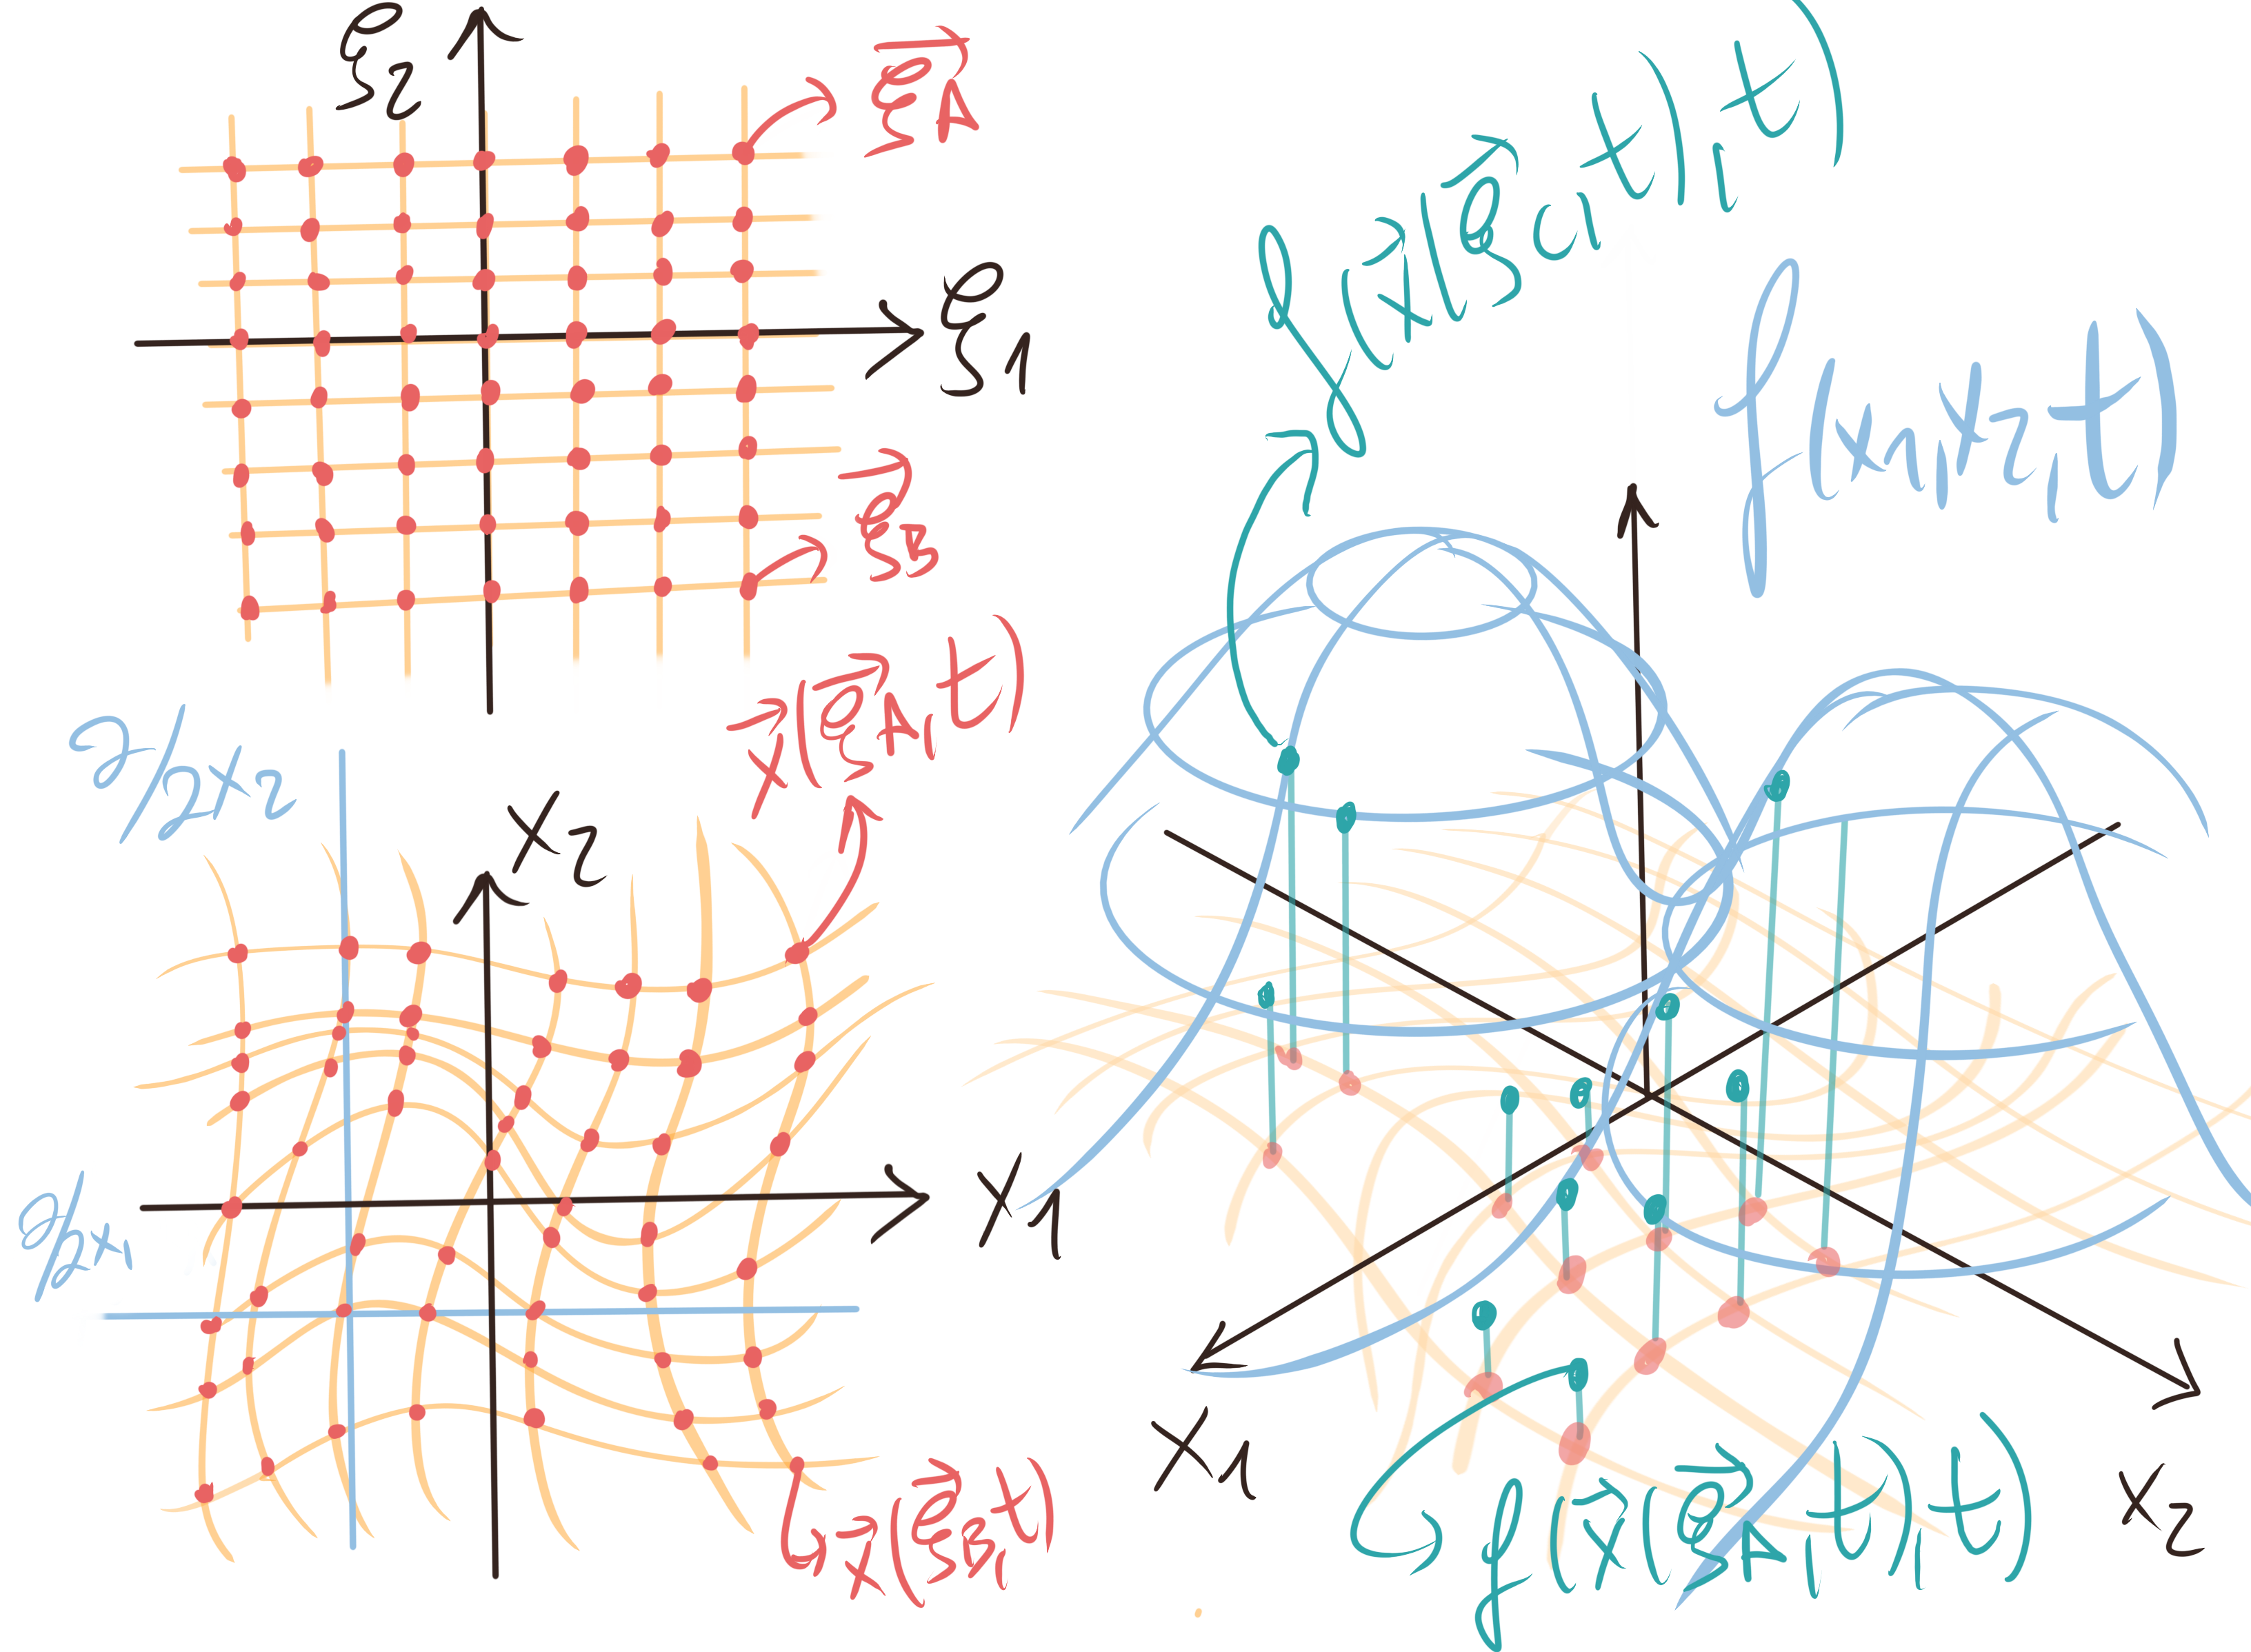
\includegraphics[width=0.64\linewidth]{azkena.png}
  \caption{Above left, the grid of fluid elements (in red) at the reference time $t_0$. Below, their positions at time $t$, note how the grid gets irregular. The partial derivatives require the knowledge of the points in the blue lines, but as it can be seen, in the unstructured grid, rarely will two fluid elements be aligned this way. In the right, we can see in blue the full function and in green the value that each fluid element carries over it. Clearly, with enough fluid elements we could reconstruct the full function.   \vspace{-0.4cm}}
  \label{fig:unstructure_fluid}
\end{figure}

Finally, note that we have still not defined a velocity field ruling the trajectories $\vec{x}(\vec{\xi},t)$. We could choose any continuous velocity field. A deeper exposition of some convenient ones will be provided in section (II.g), but in general an interesting choice will be the Bohmian velocity field we found when interpreting equation \eqref{CE}. If we choose it, the transformation $\vec{x}(\vec{\xi},t)$ will describe Bohmian trajectories:
\begin{equation}\label{ImpBohm}
\dv{}{t}x_a^\xi(t)=\frac{1}{m_a}\pdv{}{x_a}S(x_a, \vec{x}_b^{\, \xi}(t),t)\Big\rvert_{x^\xi_a(t)}=\frac{\hbar^2}{m_a}\mathbb{I}m \qty( \psi^{-1}(\vec{x}^{\, \xi}(t),t)\pdv{}{x_a}\psi(x_a, \vec{x}_b^{\, \xi}(t),t)\Big\rvert_{x^\xi_a(t)})
\end{equation}

\newpage
\section*{(II.b) The Continuity and The Hamilton-Jacobi Equations\vspace{-0.3cm}}
\addcontentsline{toc}{subsubsection}{{\bf (II.b)} The Continuity and The Hamilton-Jacobi Equations}

If we take equations \eqref{HJE} and \eqref{CE}, which are the Hamilton-Jacobi equation and the Continuity Equation for the fluid, and we evaluate them along the trajectory $\vec{x}^\xi(t)=\vec{x}(\vec{\xi},t)$, we get the following dynamical equations for the action and density over the fluid element $\vec{\xi}$:
\begin{equation}\label{CE.L}
\dv{\rho(\vec{x}^{\, \xi}(t),t)}{t}=\frac{2}{\hbar}J(\vec{x}^{\, \xi}(t),t)\ \rho(\vec{x}^{\, \xi}(t),t)
\end{equation}
\begin{equation}\label{HJE.L}
-\dv{S(\vec{x}^{\, \xi}(t),t)}{t}=G(\vec{x}^{\, \xi}(t),t)+U(\vec{x}^{\, \xi}(t),t)
\end{equation}
where we defined the {\bf correlation terms $G$ and $J$} as:
\begin{equation}\label{JL}
J(\vec{x}^{\, \xi}(t),t):=\frac{\hbar}{2\rho}\sum_{a=1}^N\qty{-\frac{1}{m_a}\pdv{}{x_a}\qty(\rho(x_a, \vec{x}_b^{\, \xi}(t),t)\ S(x_a, \vec{x}_b^{\, \xi}(t),t))\Big\rvert_{x_a^\xi(t)}+\pdv{\rho(x_a, \vec{x}_b^{\, \xi}(t),t)}{x_a}\Big\rvert_{x_a^\xi(t)}\pdv{x_a(\vec{\xi},t)}{t}}
\end{equation}
\begin{equation}\label{GL}
G(\vec{x}^{\, \xi}(t),t):=\sum_{a=1}^N\qty{\frac{1}{2m_a}\qty(\pdv{S(x_a, \vec{x}_b^{\, \xi}(t),t)}{x_a})^2\Big\rvert_{x_a^\xi(t)}-\pdv{S(x_a, \vec{x}_b^{\, \xi}(t),t)}{x_a}\Big\rvert_{x_a^\xi(t)}\pdv{x_a(\vec{\xi},t)}{t}+Q_a(x_a, \vec{x}_b^{\, \xi}(t),t)\Big\rvert_{x_a^\xi(t)}}\vspace{-0.1cm}
\end{equation}
We used the definition of the quantum potential for the degree $x_a$ given in \eqref{QP}.

As it can be seen, all the terms in both $G$ and $J$ depend on derivatives of the action and density in the Eulerian positions $\pdv{}{x_a}$, meaning they depend on the values of the action and density carried by fluid elements nearby. That is why we call them correlation terms: they are the ones introducing the coupling between the different fluid elements.

Before we jump to the interpretation of these terms, note that we can write equations \eqref{HJE.L} and \eqref{CE.L} in integral form and get the value they should have along each trajectory as:
\begin{equation}\label{JacPre}
\rho(\vec{x}^{\, \xi}(t),t)=e^{\int_{t=t_0}^t \frac{2}{\hbar}J(\vec{x}^{\, \xi}(t),t) dt}\rho(\vec{x}^{\, \xi}(t_0),t_0)
\end{equation}
\begin{equation}\label{ActPre}
S(\vec{x}^{\, \xi}(t),t)=\int_{t=t_0}^t -\qty[G(\vec{x}^{\, \xi}(t),t)+U(\vec{x}^{\, \xi}(t),t)] dt+S(\vec{x}^{\, \xi}(t_0),t_0)
\end{equation}
These two equations allow the coupled evolution of the fields $S$ and $\rho$ along the trajectories, as long as we know the correlation terms $G$ and $J$ along them. If we manage to be able to evolve $S(\vec{\xi},t)$ and $\rho(\vec{\xi},t)$, we could immediately get the full wavefunction over the trajectory as $\psi(\vec{x}^{\, \xi}(t),t)=\rho(\vec{x}^{\, \xi}(t),t)^{1/2}exp(iS(\vec{x}^{\, \xi}(t),t)/\hbar)$. In fact, we can ensemble equations \eqref{JacPre} and \eqref{ActPre} to get the time evolution of the wavefunction in an alternative way:
\begin{equation}
\psi(\vec{x}^{\, \xi}(t),t)=e^{\int_{t=t_0}^t\qty( \frac{-i}{\hbar} \qty[G(\vec{x}^{\, \xi}(t),t)+U(\vec{x}^{\, \xi}(t),t)]- \frac{2}{\hbar}J(\vec{x}^{\, \xi}(t),t) )dt}\ \psi(\vec{x}^{\, \xi}(t_0),t_0)
\end{equation}
This is sometimes called the {\bf hydrodynamical wave-function propagator}.

Now, note that we will face the same trouble that we had in the Schrödinger Equation \eqref{KinAdv}, when we try to evolve any of the present equations. In order to evaluate the quantities $\pdv{}{x_a}S(x_a, \vec{x}_b^{\, \xi}(t),t)$, $\pdv[2]{}{x_a}\rho^{1/2}(x_a, \vec{x}_b^{\, \xi}(t),t)$ on the trajectory spots (the components of the correlation terms), we need knowledge in points surrounding the fluid elements. The potential solutions will be the same:\vspace{-0.2cm}
\begin{enumerate}
\item Evolve simultaneously several fluid elements so as to numerically compute the derivatives in the unstructured grid they suppose. For this,\vspace{-0.15cm} \begin{enumerate}
\item Reconstruct each locality by fitting a sum of analytic functions locally to get the derivative symbolically or some alternative fitting technique.\vspace{-0.1cm}
\item Convert the partial derivatives with respect to space $\pdv{}{x_k}$ into derivatives with respect to the labels $\pdv{}{\xi_j}$, with the extra cost of computing the Jacobian and its determinants. We will explore the resulting equations in section (II.e). \vspace{-0.15cm}
\end{enumerate}
\item Evolve more differential equations describing the dynamics in time for the partial derivatives, conditioned along the trajectories. This will be drafted in section (II.d).
\vspace{-0.25cm}
\end{enumerate}

\subsubsection*{Understanding the G and J correlation terms}
Now, these equations and the terms correlating the fluid elements can more easily be understood if we assume the trajectories are governed by the Bohmian velocity field defined as:
\begin{equation}\label{v}
\dv{}{t}x_a^\xi(t)=\frac{1}{m_a}\pdv{}{x_a}S(x_a, \vec{x}_b^{\, \xi}(t),t)\Big\rvert_{x^\xi_a(t)}=:v_a(\vec{x}^{\, \xi}(t),t)
\end{equation}
After a pair of simplifications and re-orderings, we get that the correlation term $G$ takes the following shape:
\begin{equation}
G(\vec{x}^{\, \xi}(t),t)=\sum_{a=1}^N \frac{1}{2}m_a\qty(v_a(\vec{x}^{\, \xi}(t),t))^2+Q(\vec{x}^{\, \xi}(t),t)
\end{equation}
where we can recognize the difference between the kinetic energy of the fluid element and its quantum potential. The only thing in $G$ that depends on the rest of fluid elements is the quantum potential. Also, note that $G+U$ will yield the difference between the total kinetic energy of the fluid element and the total potential energy: it will be the {\bf Lagrangian} of the system over this particular trajectory. With this, the time evolution for the action over the fluid element would be left as:
\begin{equation}\label{HJE.L.Bohm}
\dv{}{t}S(\vec{x}^{\, \xi}(t),t)=  \sum_{a=1}^N \frac{1}{2} m_a \qty(v_k(\vec{x}^{\, \xi}(t),t) )^2 - \qty(V(\vec{x}^{\, \xi}(t),t)+ Q(\vec{x}^{\, \xi}(t),t))=: \Lg(\vec{x}^{\, \xi}(t),t)
\end{equation}
which is the classical time evolution of a system of $N$ particles, just that  here the particles are subject to a potential (the quantum potential) that depends explicitly on the density carried by other nearby possible trajectories of the system. It is purely there where the quantum effect appears, in the fact that each possible (Bohmian) trajectory of the system carries a density value that gets repelled by big density values of close trajectories in configuration space. But how does this density carried by each trajectory evolve? By doing the same assumption \eqref{v} for the velocity field, we get the convenient shape for $J$ given by:
\begin{equation}
J(\vec{x}^{\, \xi}(t),t)=-\sum_{a=1}^N \pdv{v_a(x_a, \vec{x}_b^{\, \xi}(t),t)}{x_a}\Big\rvert_{x_a^\xi(t)}
\end{equation}
which can be seen to be the negative divergence in Eulerian space for the fluid element ensemble along the trajectory of interest. We will analyse in the following section why this is a way to express that the total number of tangent Universes (or the total density) is preserved. The time evolution for the density as seen by the fluid element $\vec{\xi}$ is then:
\begin{equation}\label{CE.L.Bohm}
\dv{}{t}\rho(\vec{x}^{\, \xi}(t),t)=-\rho(\vec{x}^{\, \xi}(t),t)\sum_{a=1}^N\pdv{}{x_a} v_a(x_a, \vec{x}_b^{\, \xi}(t),t)\Big\rvert_{x_a^\xi(t)}
\end{equation}
which just expresses the fact that the divergence of Bohmian trajectories is the unique factor that can dilute or concentrate the density in the neighbourhood of a fluid element.

We can rewrite equations \eqref{HJE.L.Bohm} and \eqref{CE.L.Bohm} in integral form to get the value they should have along each Bohmian trajectory:
\begin{equation}\label{JacPre.Bohm}
\rho(\vec{x}^{\, \xi}(t),t)=e^{-\int_{t=t_0}^t \vec{\nabla}_x\cdot \vec{v}(\vec{x},t)\rvert_{\vec{x}^{\, \xi}(t)} dt}\rho(\vec{x}^{\, \xi}(t_0),t_0)
\end{equation}
\begin{equation}\label{ActPre.Bohm}
S(\vec{x}^{\, \xi}(t),t)=\int_{t=t_0}^t \Lg(\vec{x}^{\, \xi}(t),t) dt+S(\vec{x}^{\, \xi}(t_0),t_0)
\end{equation}
Together with \eqref{v}, these two equations allow the coupled evolution along Bohmian trajectories for the fields $\vec{v}$, $S$ and $\rho$. 

\subsection*{(II.a.2) G and J Correlation Potentials}
It turns out that we can get a dynamical equation for the value of the wavefunction along the trajectory using the equations of motion for the density and the action. If we note that the the action and density were obtained from the polar form of the wavefunction $\psi(\vec{x}^{\, \xi}(t),t)=\rho^{1/2}(\vec{x}^{\, \xi}(t),t)exp(iS(\vec{x}^{\, \xi}(t),t)/\hbar)$, by the product derivative rule we get that:
\begin{equation}
\dv{\psi(\vec{x}^{\, \xi}(t),t)}{t}=\frac{1}{2\rho^{1/2}(\vec{x}^{\, \xi}(t),t)}\dv{\rho(\vec{x}^{\, \xi}(t),t)}{t}e^{iS(\vec{x}^{\, \xi}(t),t)/\hbar}+\rho^{1/2}(\vec{x}^{\, \xi}(t),t)e^{iS(\vec{x}^{\, \xi}(t),t)/\hbar}\dv{S(\vec{x}^{\, \xi}(t),t)}{t}\frac{i}{\hbar}
\end{equation}
where we can introduce equations \eqref{CE.L} and \eqref{HJE.L} and reidentify the wavefunction to get:
\begin{equation}
i\hbar \dv{\psi(\vec{x}^{\, \xi}(t),t)}{t}=\qty(U(\vec{x}^{\, \xi}(t),t)+G(\vec{x}^{\, \xi}(t),t)+iJ(\vec{x}^{\, \xi}(t),t))\psi(\vec{x}^{\, \xi}(t),t)
\end{equation}
which is an equation describing the time evolution of the wavefunction along the trajectory in a linear way. Note that the equation is in reality non-linear since the correlation terms depend on the magnitude and phase of the unknown. Also, we now see that we could call $G$ and $J$ correlation {\bf potentials}, since they can be interpreted as a (complex) potential energy driving the wavefunction over the trajectory.

Finally, note the functional relationship between the two kinds of correlation terms seen so far:
\begin{equation}
\qty(G(\vec{x}^{\, \xi}(t),t)+iJ(\vec{x}^{\, \xi}(t),t))\psi(\vec{x}^{\, \xi}(t),t)=K(\vec{x}^{\, \xi}(t),t)+A(\vec{x}^{\, \xi}(t),t)
\end{equation}

\section*{(II.f) The Bohmian Newton's Second Law}
\addcontentsline{toc}{subsubsection}{{\bf (II.f)} The Bohmian Newton's Second Law}
If we take the Hamilton-Jacobi Equation in the fully Eulerian frame \eqref{HJE} and do the partial derivative $\pdv{}{x_k}$ at both sides, by assuming the particular Bohmian velocity field for the trajectories, given by \eqref{v}, and assuming enough regularity for $S$, we arrive at:
\begin{equation}
\pdv{}{t}\pdv{}{x_k}S(\vec{x},t)+\sum_{j=1}^N\pdv{}{x_j}\pdv{}{x_k}S(\vec{x},t)\cdot v_j(\vec{x},t)=-\pdv{}{x_k}\qty(V(\vec{x},t)+Q(\vec{x},t))
\end{equation}
If we evaluate $\vec{x}$ in the Lagrangian frame $\vec{x}(\vec{\xi},t)$, we immediately find (assuming \eqref{v}):
\begin{equation}
m_k\dv{}{t}v_k(\vec{x}^{\, \xi}(t),t)=m_k\dv[2]{}{t}x^\xi_k(t)=-\pdv{}{x_k}\qty[V(\vec{x}^{\, \xi}(t),t)+Q(\vec{x}^{\, \xi}(t),t) ]\vspace{-0.1cm}
\end{equation}
This is Newton's Second Law for each fluid element $\vec{\xi}$. This equation can be evolved coupled with the continuity equation \eqref{CE.L} in order to know the evolution of the density $\rho$ and the Bohmian velocity field. In this representation however, we will require to compute the spatial derivative of the quantum potential $Q$, which was already a problematic term due to the $\pdv[2]{}{x_j}R(\vec{x},t)$ it contains. Therefore, even if the equation is very insightful in a theoretical basis, legitimising Bohmian trajectories, for numerical purposes it is more stable to use the equations of motion of (II.a) or (II.b).\vspace{-0.2cm}

%\subsection*{(II.c) Basis Set Expansions}
%\addcontentsline{toc}{subsubsection}{{\bf (II.c)} Basis Set Expansions?}

\section*{(II.d) Dynamic Equations for Partial Derivatives\vspace{-0.2cm}}
\addcontentsline{toc}{subsubsection}{{\bf (II.d)} Dynamic Equations for Partial Derivatives}


\subsection*{(II.d.a) Dynamics of Partial Derivatives For the Wavefunction\vspace{-0.1cm}}
%\addcontentsline{toc}{subsubsection}{(II.d.a) Dynamics of Partial Derivatives For the Wavefunction}

If we go back to the coupled system of (infinite) linear differential equations \eqref{infchain.SE}, we will notice that there is no partial derivative with respect to space $x_k$ in any place. This means that we can actually evolve a single fluid element by directly evaluating $\vec{x}=\vec{x}(\vec{\xi},t)$. For this, we must first note the chain rule \eqref{chainRuler} in order to get the time derivative as seen by the fluid element $\vec{\xi}$.
%that by the chain rule, given a differentiable function $f(\vec{x},t)$:
%\begin{equation}\label{ruler}
%\pdv{f(\vec{x},t)}{t}\Big\rvert_{x(\xi,t)} = \dv{f(\vec{x}(\vec{\xi},t),t)}{t}-\sum_{s=1}^N \pdv{f(\vec{x},t)}{x_s}\Big\rvert_{x_s(\vec{\xi},t)}\pdv{x_s(\xi,t)}{t}
%\end{equation}
%In the notation we defined in \eqref{defPdv}, we saw $\pdv{f(\vec{x},t)}{x_s}=f_{(0,...,1,...,0)}(\vec{x},t)$ (with the array full of 0-s except for a 1 in the $s$-th position). Then:
%\begin{equation}\label{matrialTimePdv}
%\pdv{f(\vec{x},t)}{t}\Big\rvert_{x(\xi,t)} = \pdv{f(\xi,t)}{t}-\sum_{s=1}^N f_{(0,...,1,...,0)}(\xi,t) \pdv{x_s(\xi,t)}{t}
%\end{equation}
Then, retaking the definition \eqref{defPdv}, this would leave \eqref{infchain.SE} in the Lagrangian frame as:\vspace{-0.1cm}
\begin{equation}\label{infchain.SE.L}
i\hbar \pdv{}{t}\psi_{(j_1,...,j_N)}(\xi,t)=\sum_{s=1}^N\qty[-\frac{\hbar^2}{2m_s}\psi_{(j_1,...,2+j_s,...,j_N)}+i\hbar \psi_{(j_1,...,1+j_s,...,j_N)} \pdv{x_s(\vec{\xi},t)}{t}]+\vspace{-0.1cm}
\end{equation}
$$
+\sum_{k_1=0}^{j_1}\cdots\sum_{k_N=0}^{j_N} b(j_1,k_1)\cdots b(j_N,k_N)U_{(j_1-k_1,...,j_N-k_N)}\psi_{(k_1,...,k_N)}
$$
where all the functions have arguments $(\vec{\xi},t)$.

{\em A priori}, this is an infinite system of coupled {\bf linear} differential equations. However, if we assume that at a certain $J$, $\pdv[J]{\psi(\vec{x},t)}{x_k}\Big\rvert_{x(\xi,t)}\simeq 0$  $\forall k$, we are left with $J^N$ coupled linear equations. Doing this approximation, we are assuming that the wavefunction in the immediate locality of the fluid element has a roughly constant derivative of $J$-th order. Contrary to the Eulerian case, we are not assuming this for the whole configuration space. Thus depending on the chosen trajectory, a low $J$ may not be a problematic assumption. The best point about this mehtod is that this equation system would allow us to compute the wavefunction and trajectory of a {\bf single} fluid element $\vec{\xi}$. With no need to know the partial derivatives in configuration-space $x_k$, there is no need to couple other trajectories to this one.

Certainly, the main problem of this method is that we will need to choose the truncation $J$, which if chosen to be too small, would make the trajectory blind to nodal points and fluctuating regions that are not in its immediate vicinity but should influence the trajectory.\vspace{-0.1cm}

\subsection*{(II.d.b) Dynamics of Partial Derivatives For the Density and Action\vspace{-0.1cm}}
%\addcontentsline{toc}{subsubsection}{(II.d.b) Dynamics of Partial Derivatives}

If we now go back to equations \eqref{infchain.CE} and \eqref{infchain.HJE}, we will see that it is possible to evaluate $\vec{x}=\vec{x}(\vec{\xi},t)$ directly in the partial differential equations ruling the dynamics of the spatial derivatives of $C$ and $S$ as well (where $C(\vec{x},t)=log(\rho(\vec{x},t))/2$). Noting back \eqref{chainRuler}, we can see that the time evolution of the field $C$ (thus $\rho$) and all of its derivatives in configuration space $x_k$, over any single fluid element $\vec{\xi}$ follows:\vspace{-0.1cm}
\begin{equation}\label{infchain.CE.L}
\pdv{}{t}C_{(j_1,...,j_N)}(\xi,t)=-\sum_{s=1}^N \Bigg(i\hbar C_{(j_1,...,1+j_s,...,j_N)}\pdv{x_s(\vec{\xi},t)}{t} + \frac{1}{m_s} \Bigg[S_{(j1,...,2+j_s,...,jN)}(\vec{x},t)+
\end{equation}
$$
+2 \sum_{k_1=0}^{j_1}\cdots\sum_{k_N=0}^{j_N} b(j_1,k_1)\cdots b(j_N,k_N)C_{(j_1-k_1,...,1+j_s-k_s,...,j_N-k_N)}S_{(k_1,...,1+k_s,...,k_N)} \Bigg]\bigg)
$$
While the field $S$ and all its derivatives in configuration space, follow over any single fluid element $\vec{\xi}$:\vspace{-0.1cm}
\begin{equation}\label{infchain.HJE.L}
-\pdv{}{t}S_{(j_1,...,j_N)}(\xi,t)=V_{(j1,...,jN)}+\sum_{s=1}^N\Bigg\{ i\hbar S_{(j_1,...,1+j_s,...,j_N)}\pdv{x_s(\vec{\xi},t)}{t}-\frac{\hbar^2}{2m_s} \Bigg[ C_{(j1,...,2+j_s,...,jN)}+\vspace{-0.1cm}
\end{equation}
$$
+\sum_{k_1=0}^{j_1}\cdots\sum_{k_N=0}^{j_N} b(j_1,k_1)\cdots b(j_N,k_N) \Bigg( C_{(j_1-k_1,...,1+j_s-k_s,...,j_N-k_N)}C_{(k_1,...,1+k_s,...,k_N)} \vspace{-0.1cm}
$$
$$
-S_{(j_1-k_1,...,1+j_s-k_s,...,j_N-k_N)}S_{(k_1,...,1+k_s,...,k_N)}  \Bigg)\Bigg]\Bigg\}
$$
Again, these equations allow us the computation of the wavefunction and the trajectory of a single fluid element at any time. For a numerical implementation however, we will need to assume that at a certain $J$, $\pdv[J]{f(\vec{x},t)}{x_k}\Big\rvert_{\vec{x}(\vec{\xi},t)}\simeq 0$ for $f\in\{ C,S\}$. This means we will need to assume that in the locality of the trajectory the $C$ amplitude's (and the density's) and the action's curvatures get close to zero.

Unlike equation \eqref{infchain.SE.L}, these systems of equations are not linear.

\newpage
\section*{{\em Parenthesis: }Fundamental Intuitions about the Diffeomorphism $\vec{x}(\vec{\xi},t)$}
\addcontentsline{toc}{subsubsection}{\em Parenthesis: Fundamental Intuitions about the Diffeomorphism $\vec{x}(\vec{\xi},t)$}

Before continuing to the next sections, we will open a little parenthesis to review the relevant concepts that one must have clear when talking about the trajectory bundle of a fluid. These trajectories are given by a transformation $\vec{x}(\vec{\xi},t)$ that maps each fluid element in the label space $\vec{\xi}$, which we decided to identify with the initial position (in configuration-space) of each fluid element ($\vec{x}(\vec{\xi},t=t_0)=\vec{\xi}$), to the position of the fluid element at time $t$. For the reasons we have already seen, it must be a diffeomorphism, a continuous, differentiable and invertible map. \vspace{-0.3cm}
\subsection*{ Covariant Tangent Vectors \vspace{-0.3cm}}
Let us first realize what the vectors $\pdv{\vec{x}(\vec{\xi},t)}{\xi_k}$ are. For this, lets define a {\bf iso-label curve} or iso-curve. It is the image of the straight line corresponding to the $\xi_k$ axis in the original label space, as can be seen in Figure \ref{fig:isoline}.  It is the curve that shows where the fluid elements that were initially in that straight line are at time $t$. It is thus the curve defined by fixing all spatial variables of $\vec{\xi}$ except for $\xi_k$, which if varied, shapes the parametric curve $\vec{x}(\xi_k;\xi_1,...,\xi_{k-1},\xi_{k+1},...,\xi_N,t)$. Since, $\vec{x}(\vec{\xi},t)$ must be continuous to be a valid diffeomorphism, the fluid elements that were initially close in configuration space, must remain close, but can now be distributed in a curved manner instead of a straight line. This means that, the "distance" between these close points can be contracted or dilated as we will see in a moment.
\begin{figure}[h!]
  \centering
    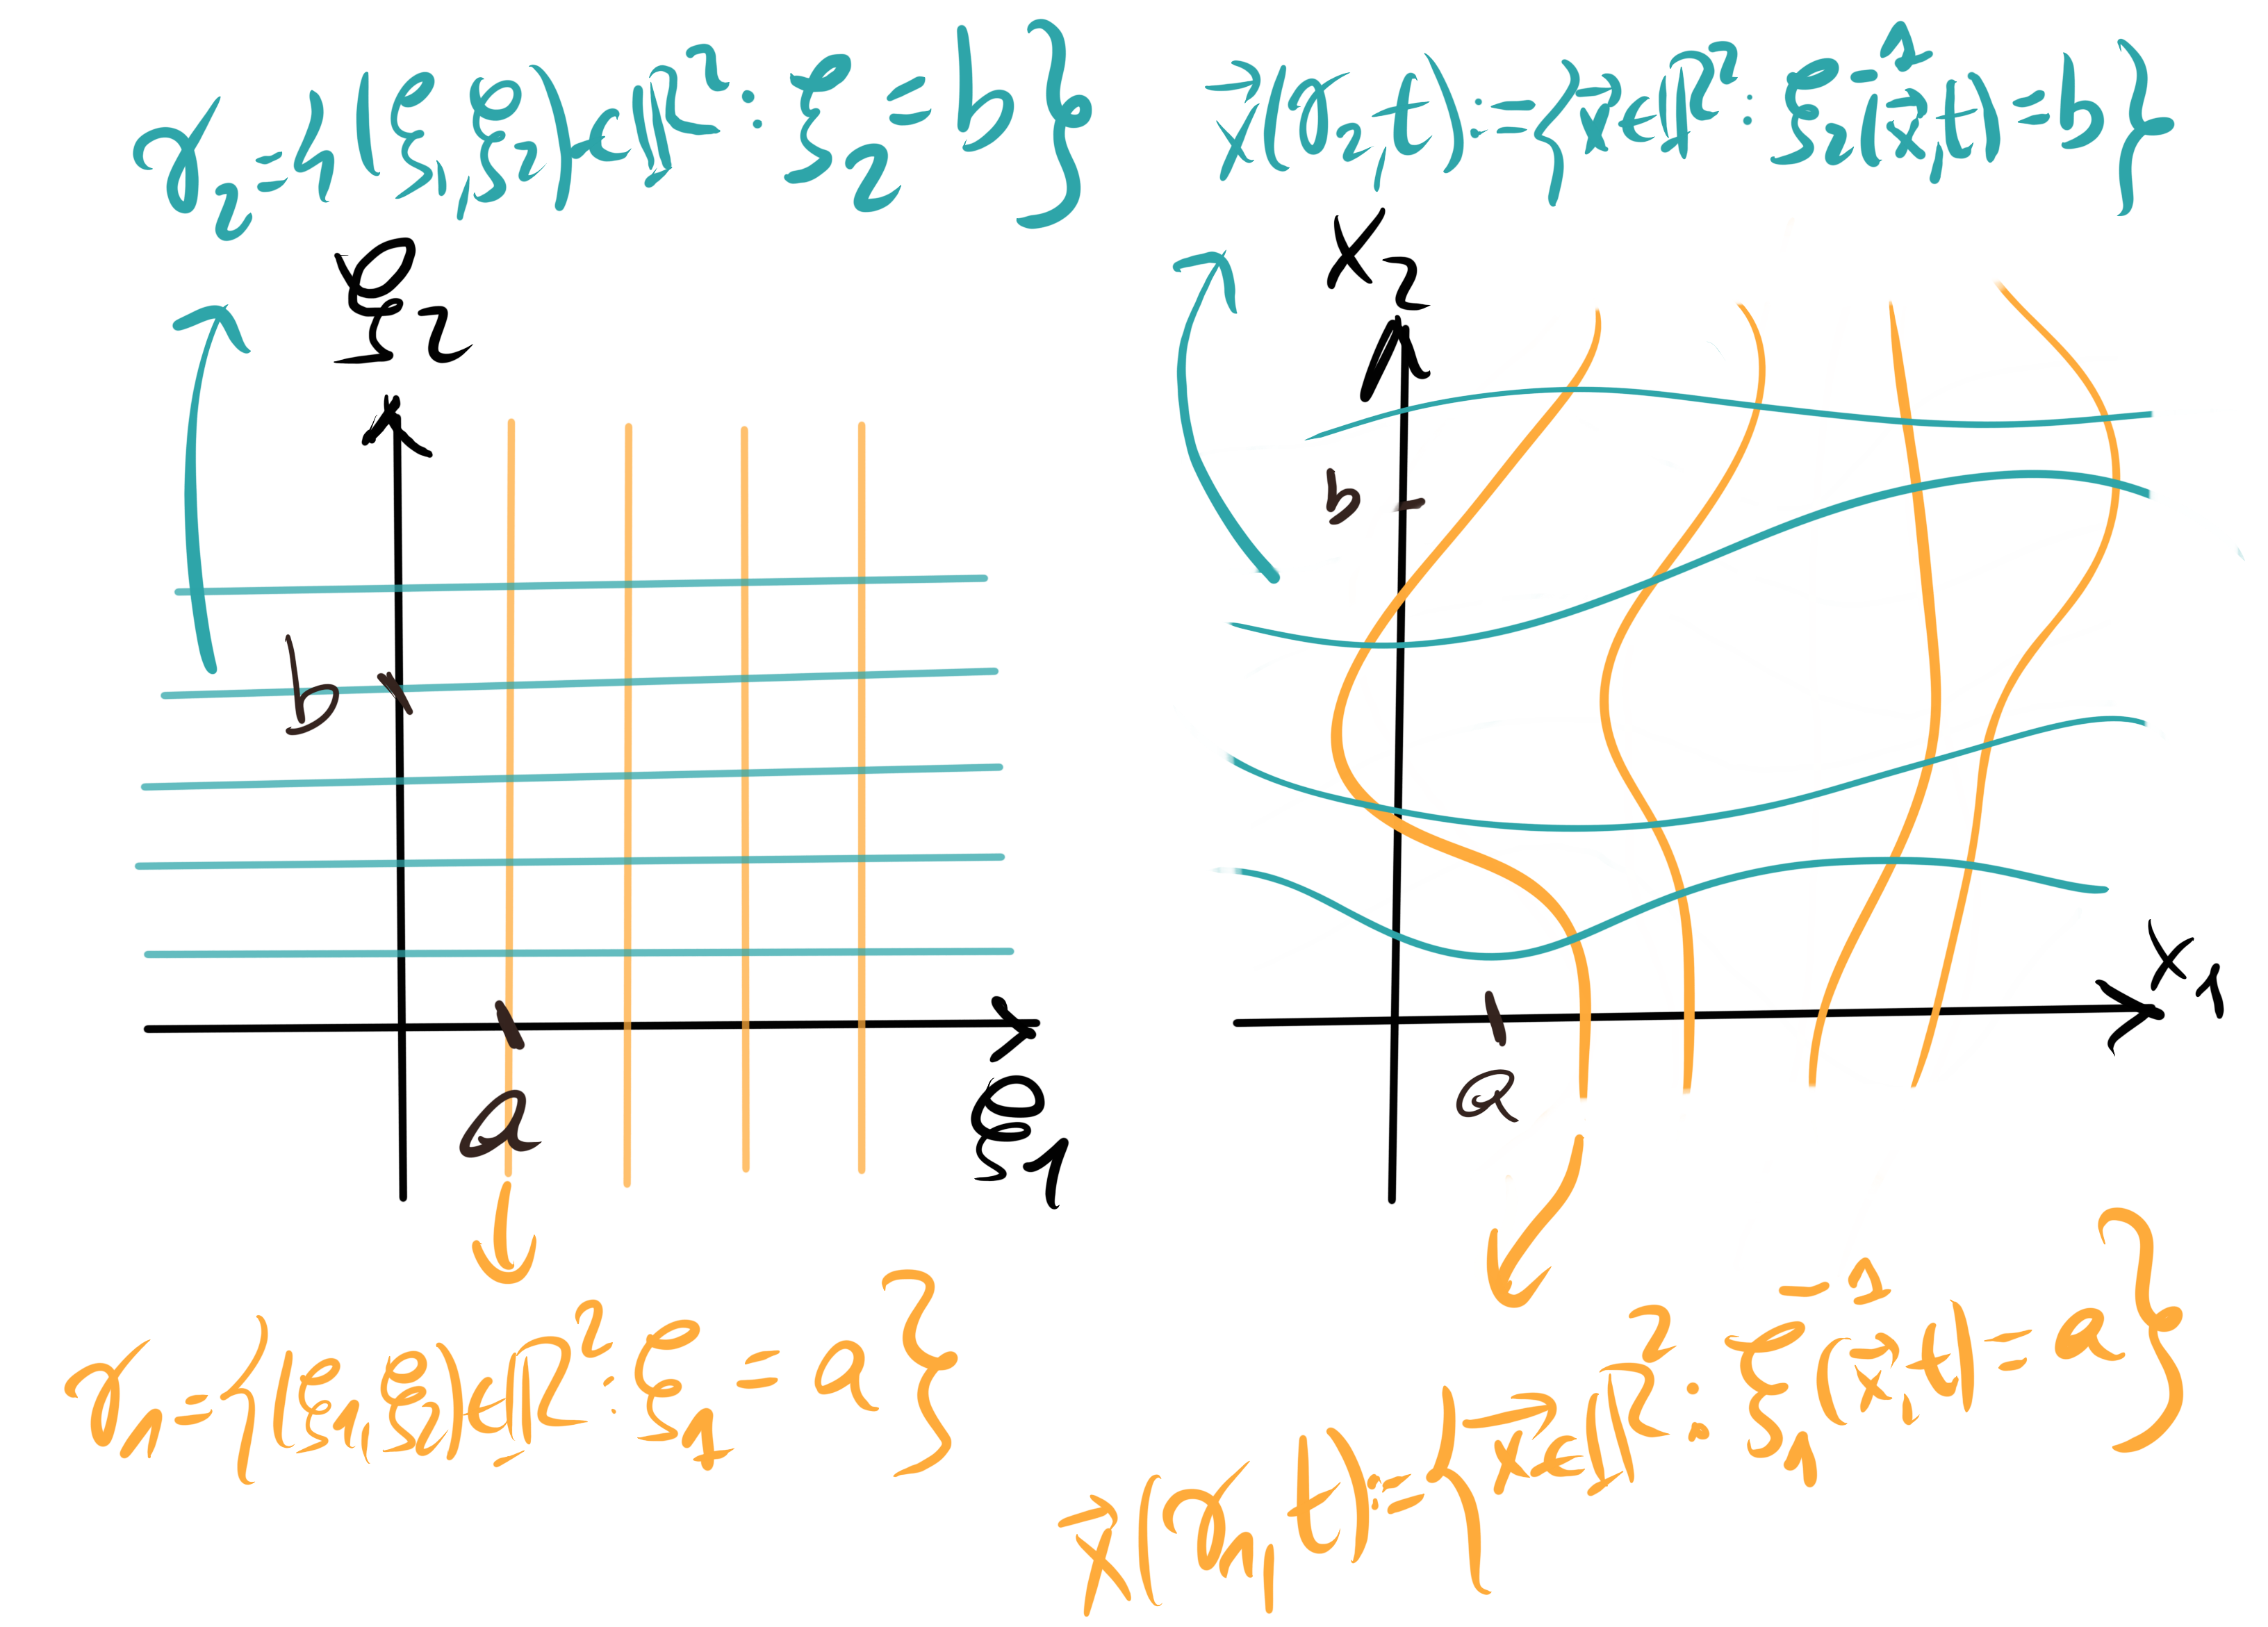
\includegraphics[width=0.65\linewidth]{5isolines.png}
  \caption{Depiction of the iso-label curves. They are the set of points that have one of the label space coordinates fixed at a same number. Considering that the label space represents the initial positions for the fluid elements, the iso-curve at any time $t$ represents the set of positions where the fluid elements that were once aligned have moved to. Since their displacement is given by a diffeomorphism, the iso-label curves will be continuous curves at all times. The angles between the iso-curves do not need to be preserved however. }
  \label{fig:isoline}
\end{figure}

 Then, the vectors $\pdv{\vec{x}(\vec{\xi},t)}{\xi_k}$, following the definition of partial derivative:
\begin{equation}
\pdv{\vec{x}(\vec{\xi},t)}{\xi_k}=\lim_{\Delta \xi \rightarrow \infty} \frac{\vec{x}(\xi_1,...,\xi_k+\Delta \xi,...,\xi_N,t)-\vec{x}(\xi_1,...,\xi_k,...,\xi_N,t,t)}{\Delta \xi}
\end{equation}
are locally tangent to the iso-label curves at each time, as can be graphically intuited from Figure \ref{fig:covariant}. This is why we call them, {\bf covariant tangent vectors}. 

Then, note that set of $N$ vectors $\{\pdv{\vec{x}(\vec{\xi},t)}{\xi_1},...,\pdv{\vec{x}(\vec{\xi},t)}{\xi_N} \}$ at each point $\vec{x}(\vec{\xi},t)$, shapes locally the vector basis to which the initial orthogonal grid surrounding $\vec{\xi}$ has been morphed.
\begin{figure}[h!]
  \centering
    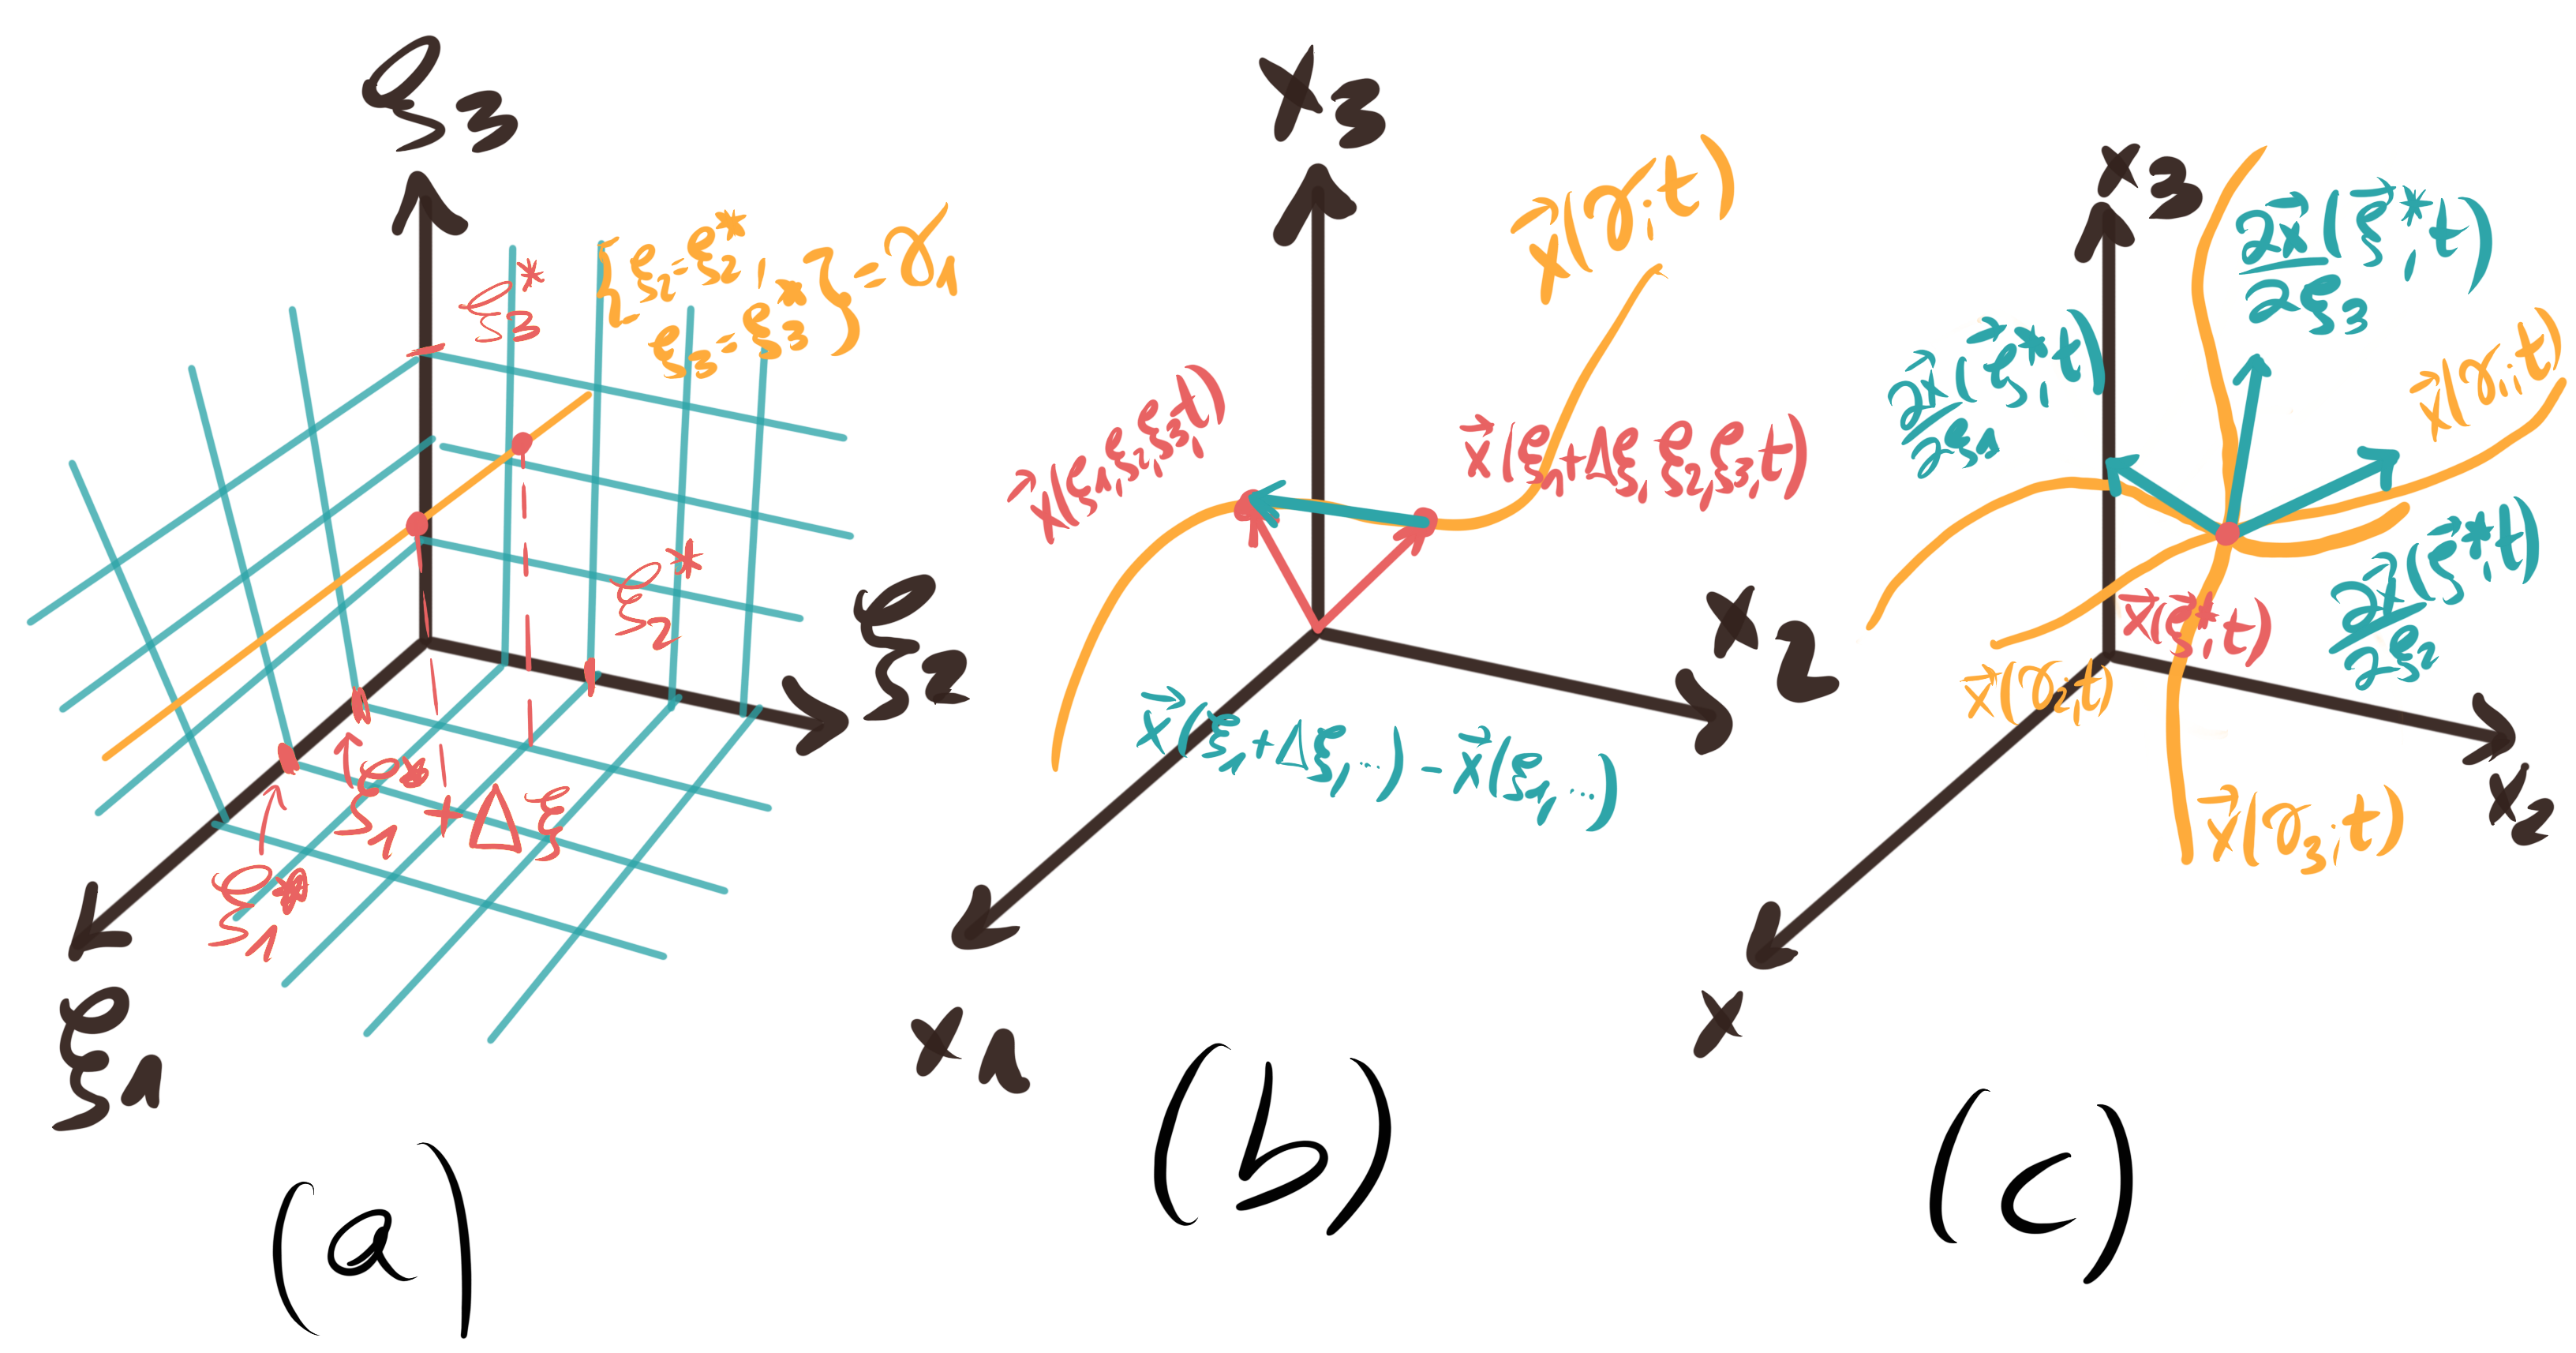
\includegraphics[width=0.75\linewidth]{3covariant_tangent_vectors.png}
  \caption{{\bf (a)} The two red dots depict the label space positions (initial positions) for two elements with the same $\xi_2, \xi_3$ coordinates but a distance in $\xi_3$ of $\Delta \xi$. Notice the yellow iso-line $\gamma_1$ that passes crossing them both.\\ {\bf (b)} The same two points but in their configuration space positions after a time $t$ has passed. Note that the iso-line $\gamma_1$ has been curved with their motion. Note however that in any time, the vector linking the two trajectories $\vec{x}(\xi_1+\Delta\xi,\xi_2,\xi_3)-\vec{x}(\xi_1,\xi_2,\xi_3)$, if $\Delta \xi$ is made sufficiently small, will be tangent to the yellow iso-$\xi_1$ label curve at the point $\vec{x}(\xi_1,\xi_2,\xi_3)$. If we take this difference, divide it by $\Delta \xi$ and make it tend to zero $\Delta \xi\rightarrow 0$, in the limit we will get the locally tangent vector to the iso-curve $\xi_1$ the magnitude of which expresses the rate of change of the arc-length of the iso-curve at that point. This is a covariant tangent vector.\\ {\bf (c)} Note that we could do the same for the three directions in label space, to get the three covariant tangent vectors, tangent to each of the iso-label curves crossing the point. Since the Jacobian determinant for a diffeomorphism must be non zero, these vectors must be linearly independent, forming a basis of the vector space. }
  \label{fig:covariant}
\end{figure}

\subsection*{The Jacobian Matrix}
We define the Jacobian matrix of $\vec{x}(\vec{\xi},t)$ with respect to the label space $\vec{\xi}$ as the matrix that has the covariant tangent vectors as columns (or the matrix of all the first order partial derivatives of $\vec{x}(\vec{\xi},t)$):
\begin{equation}
D_\xi\vec{x}(\vec{\xi},t):=\begin{pmatrix}
\pdv{x_1(\vec{\xi},t)}{\xi_1} & \cdots & \pdv{x_1(\vec{\xi},t)}{\xi_N}\\
\vdots&\ddots&\vdots \\
\pdv{x_N(\vec{\xi},t)}{\xi_1} & \cdots & \pdv{x_N(\vec{\xi},t)}{\xi_N}
\end{pmatrix}=\begin{pmatrix}
|& &|\\
\pdv{\vec{x}(\vec{\xi},t)}{\xi_1} & \cdots & \pdv{\vec{x}(\vec{\xi},t)}{\xi_N}\\
|& &|
\end{pmatrix}
\end{equation}
Note that since the transformation $\vec{x}(\vec{\xi},t)$ must be a diffeomorphism, the Jacobian matrix is well defined. This is why we know that the covariant tangent vectors were defined in the first place. In fact, we will see from its interpretation that the matrix must be non-singular, meaning the covariant tangent vectors shape a vector basis in any point $\vec{\xi}$ and time $t$.

We can interpret this matrix, which will be different at each point $(\vec{\xi},t)$, as the matrix of a linear application that takes vectors in an initial canonical basis and sends them to the basis of covariant tangent vectors at the position $\vec{x}(\vec{\xi},t)$. To see what this really means, let us write the Taylor expansion of $\vec{x}(\vec{\xi},t)$ around a certain fluid element of interest $\vec{\xi}^*$:
\begin{equation}
\vec{x}(\vec{\xi},t)=\vec{x}(\vec{\xi}^*,t)+D_{\xi}\vec{x}(\vec{\xi}^*,t)\cdot (\vec{\xi}-\vec{\xi}^*)+o(||\vec{\xi}-\vec{\xi}^*||^2)
\end{equation}
For $\vec{\xi}\rightarrow \vec{\xi}^*$ (that is, for all fluid elements close enough to $\vec{\xi}^*$ at the initial time), neglecting second order terms, we find that:
\begin{equation}
\vec{x}(\vec{\xi},t)-\vec{x}(\vec{\xi}^*,t)\simeq D_{\xi}\vec{x}(\vec{\xi}^*,t)\cdot (\vec{\xi}-\vec{\xi}^*)
\end{equation}
As it can be seen in Figure \ref{fig:JacobMatrix}, this means the Jacobian matrix is the linear application that best approximates in each neighbourhood $\vec{\xi}$ the effect of the transformation $\vec{x}(\vec{\xi},t)$ at each time. Interpreting the Jacobian matrix as the matrix of this linear application, we see that it sends the unit orthogonal vectors around each $\vec{\xi}$ to the covariant tangent vectors in $\vec{x}(\vec{\xi},t)$. See this depicted in Figure \ref{fig:localContinuum}. Then it must also encode the conversion of a local unit cube of fluid elements in $\vec{\xi}$ at $t=t_0$, to the local parallelogram that the elements of the cube shape at time $t$. If we knew the volume increase factor of this conversion, we would know the amount by which the fluid elements that were initially close to $\vec{\xi}^*$ are dilated or contracted. In fact, with this linear application matrix idea, we can now understand that the magnitude of each covariant tangent vector $||\pdv{\vec{x}(\vec{\xi},t)}{\xi_k}||$ gives us the separation increase factor at time $t$ of the distance between the fluid element $\vec{\xi}^*$ and the elements $\vec{\xi}$ that were aligned with it in the $\xi_k$ axis at time $t_0$.

\begin{figure}[h!]
  \centering
    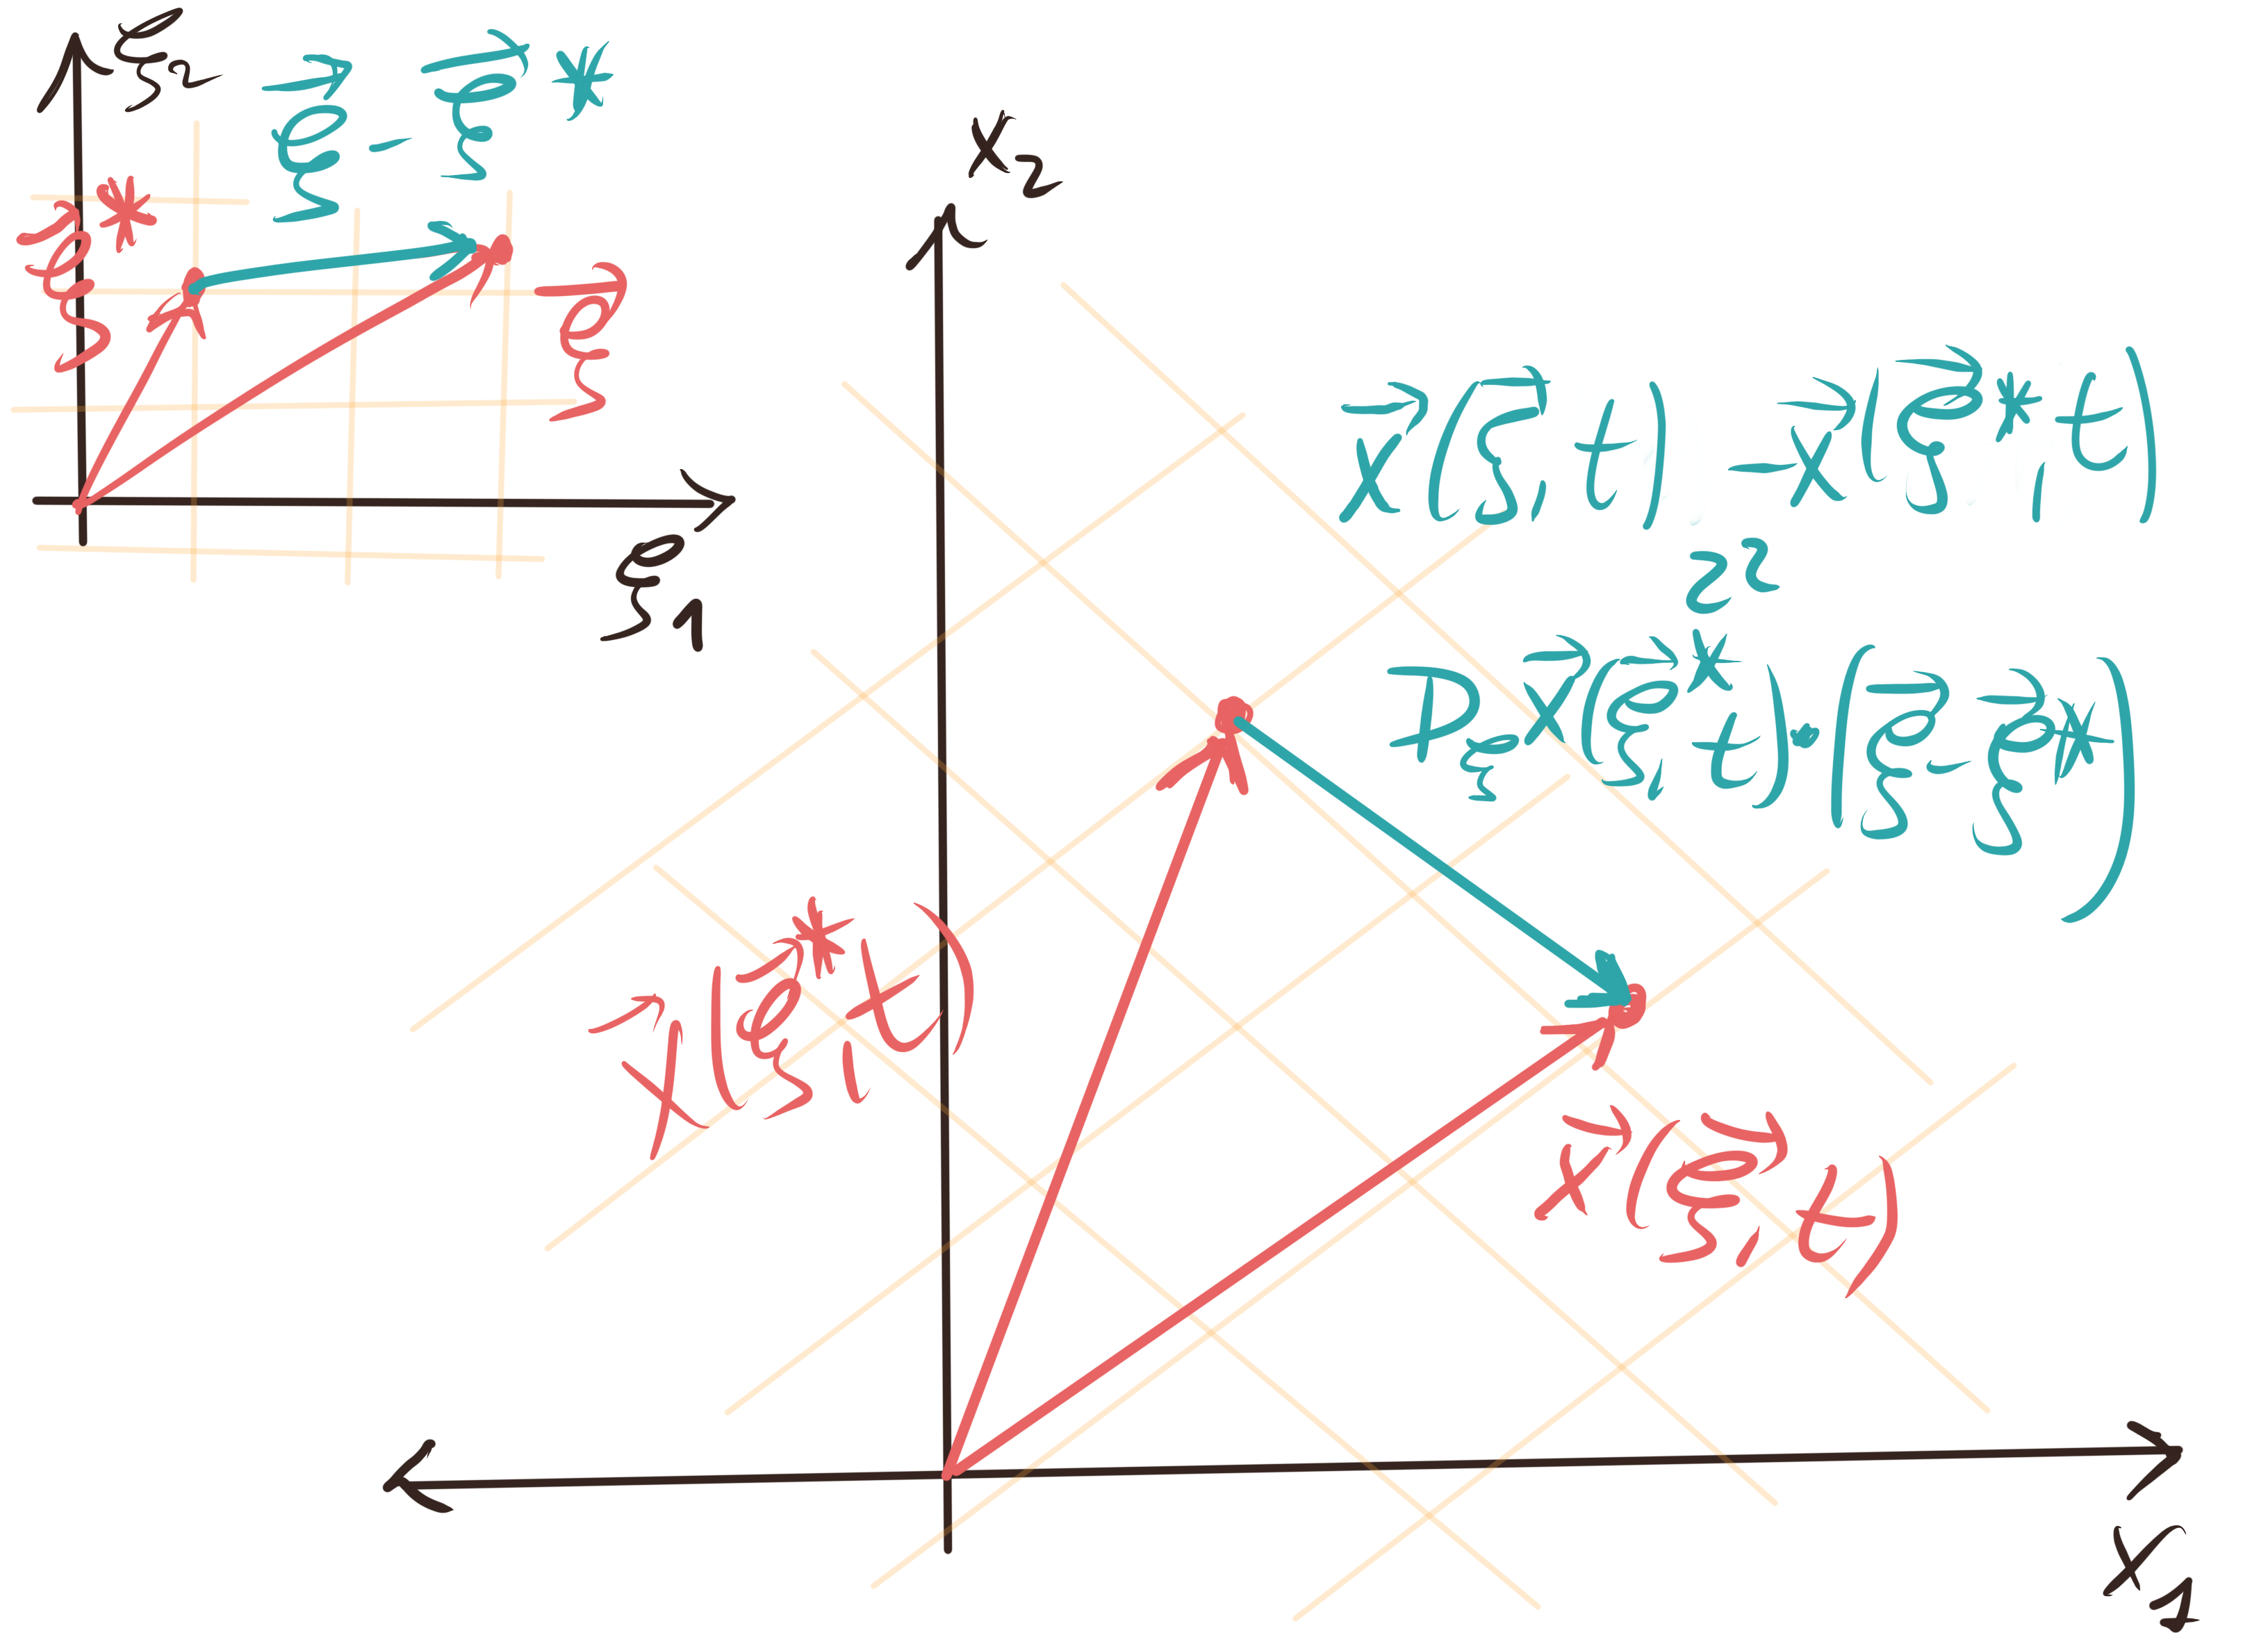
\includegraphics[width=0.57\linewidth]{2Jacob_as_lin_app.png}
  \caption{Up left a depiction of the label space vector $\vec{\xi}-\vec{\xi}^*$, which is the position vector of the fluid element $\vec{\xi}$ relative to the fluid element $\vec{\xi}^*$ at time $t_0$. Below the depiction of the relative position vector at time $t$: $\vec{x}(\vec{\xi},t)-\vec{x}(\vec{\xi}^*,t)$. If $\vec{\xi}\rightarrow \vec{\xi}^*$, this relative position vector at time $t$ should be roughly the same vector as the one to which the linear application matrix $D_\xi \vec{x}(\vec{\xi},t)$ sends the initial relative vector $\vec{\xi}-\vec{\xi}^*$. The closer the fluid elements the less erroneous it should be, until in the immediate locality of $\vec{\xi}^*$, the Jacobian matrix exactly determines the transformation of the fluid as a linear application (centred at the point $\vec{\xi}^*$). \vspace{-0.1cm} }
  \label{fig:JacobMatrix}
\end{figure}

\begin{figure}[h!]
  \centering
    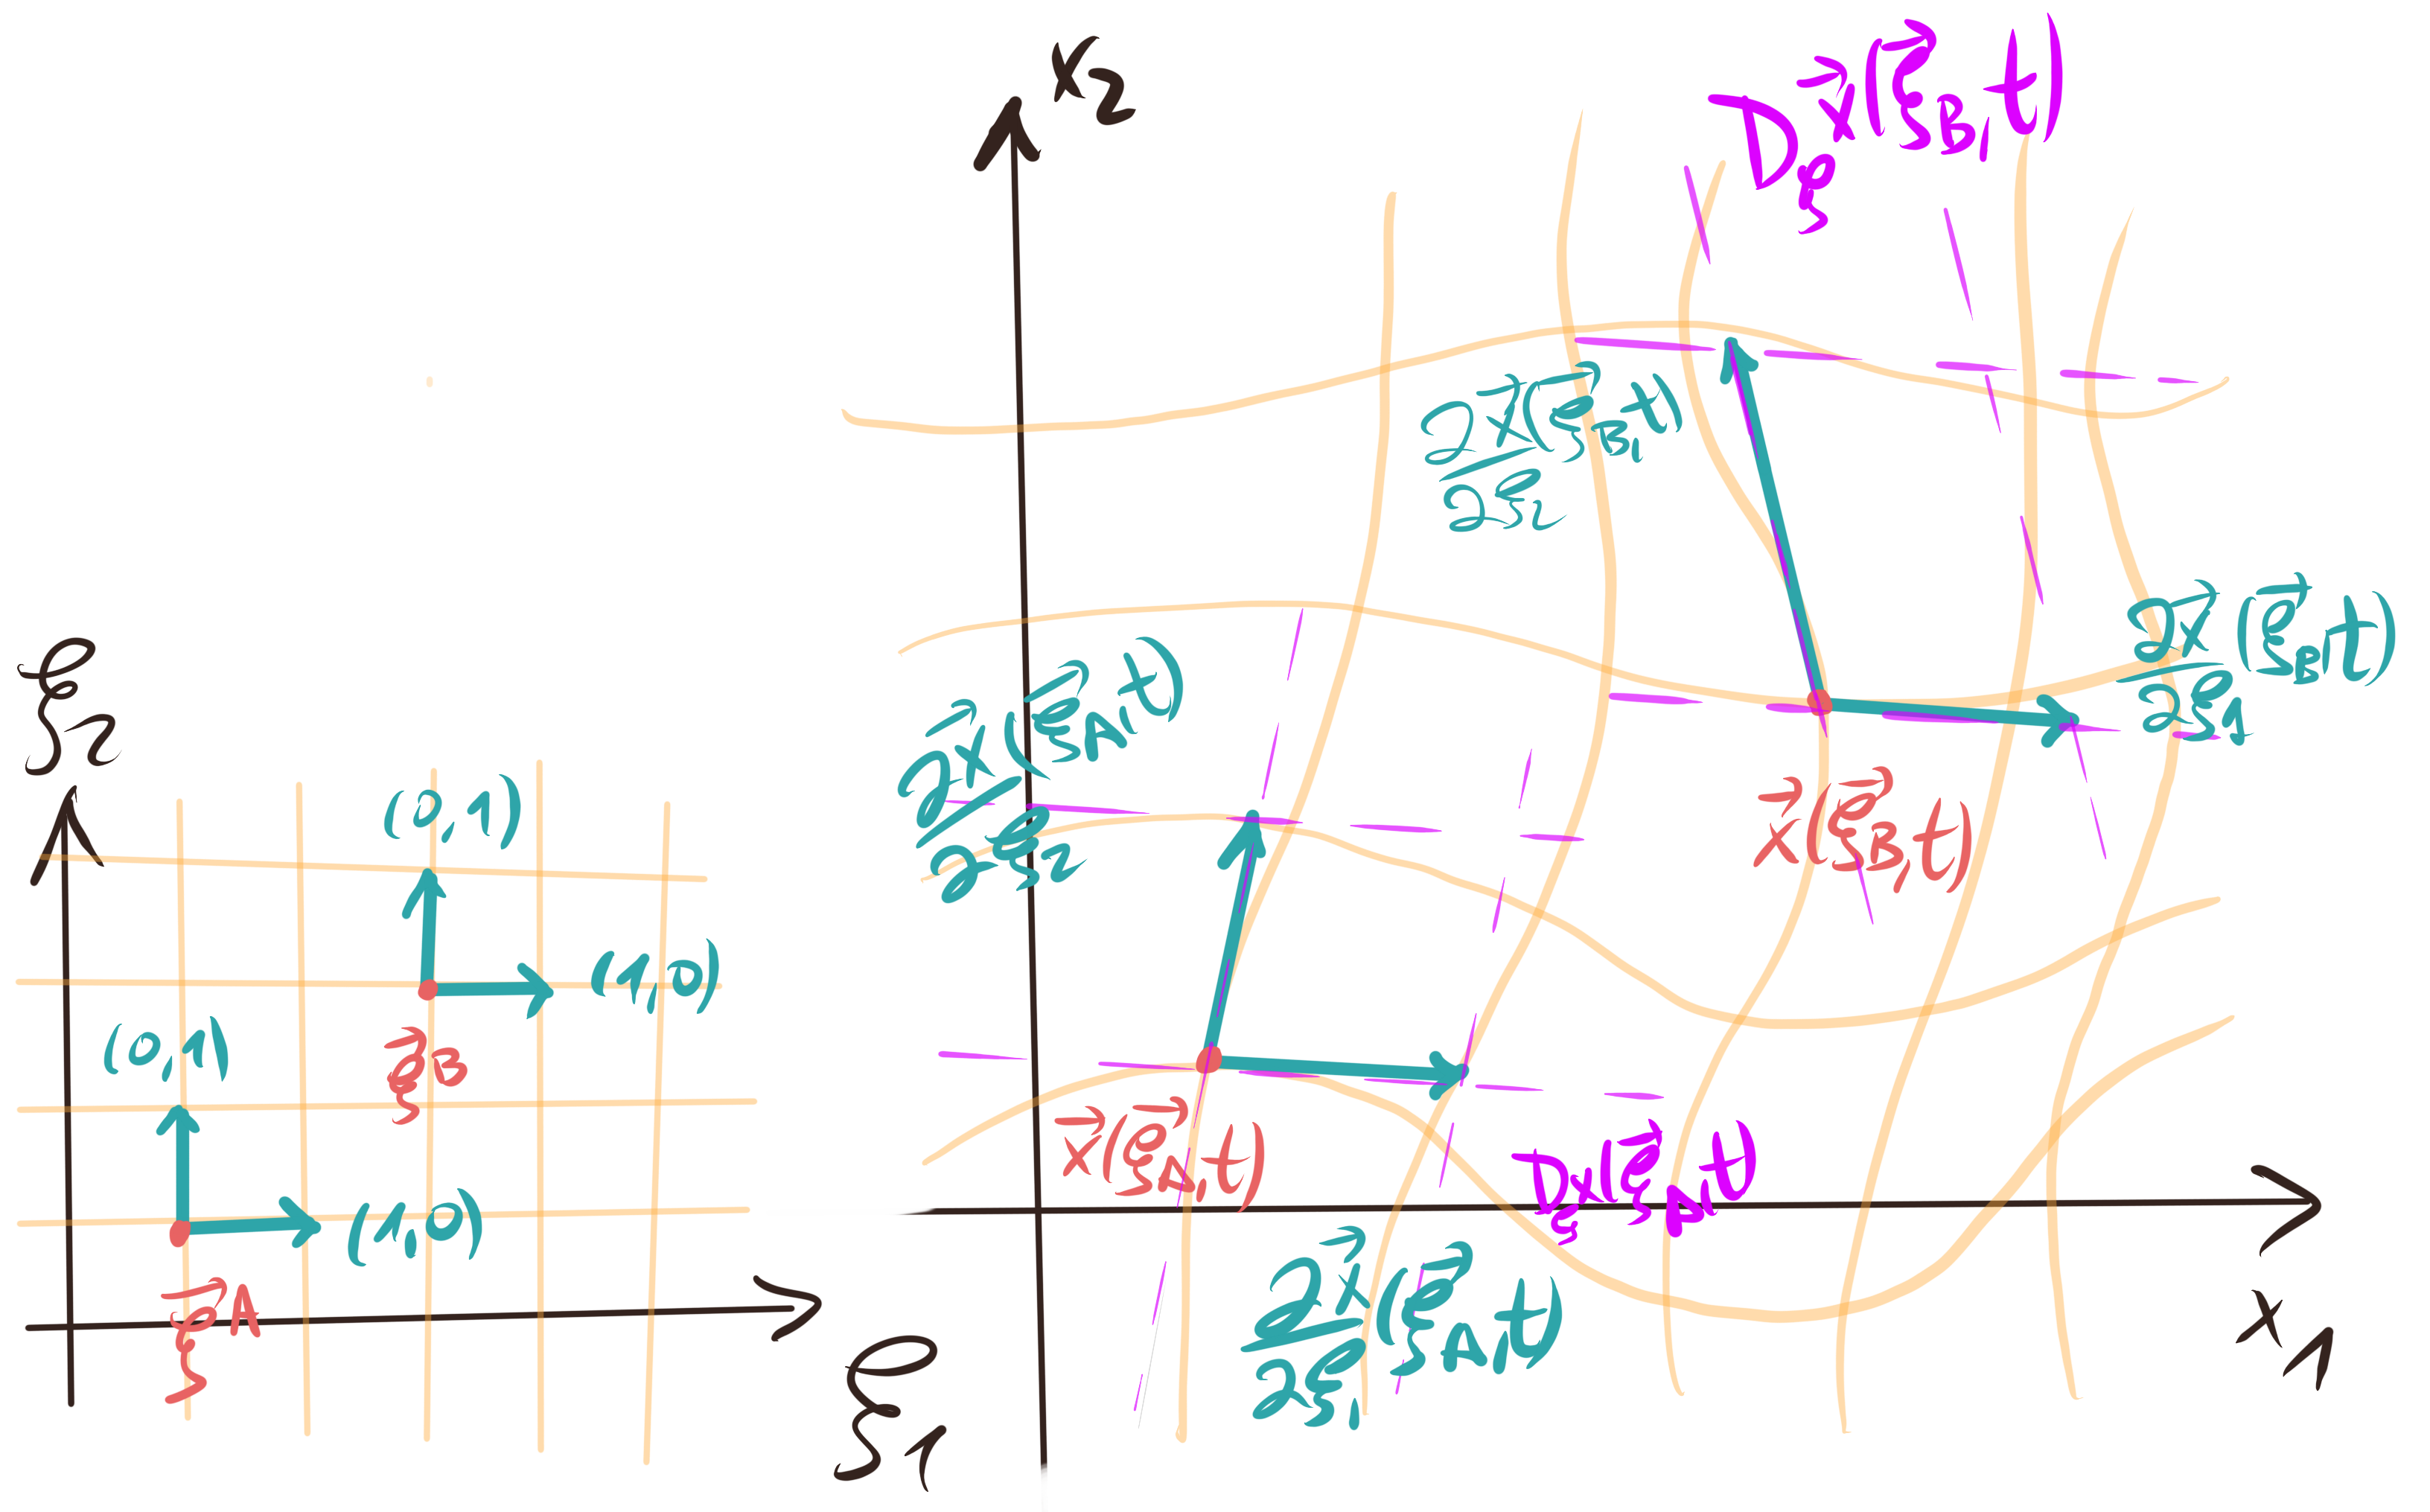
\includegraphics[width=0.65\linewidth]{4each_locality.png}
  \caption{A depiction of how at each time $t$ and each point of label space $\vec{\xi}$, there is a linear application $D_\xi\vec{x}(\vec{\xi},t)$, which locally gives the transformation that best fits the distortion of the fluid mesh. In particular, the linear application sends the canonical unit vectors (centred at each $\vec{\xi}$), in green in the left, to the basis of covariant tangent vectors, green in the right. This is nothing but a restatement that the covariant basis vectors must be locally tangent to the iso-label curves, in yellow. These curves are directed by the canonical basis vectors in the label space (where they are straight orthogonal lines) and are directed by the continuity of covariant tangent vectors in the general configuration space at time $t$. We can see in pink how the Jacobian matrix of each point, as a linear application, is precise in the immediate vicinity of the points (there its effect matches the yellow curves), but get more and more wrong as we get further away from the point in which we computed the matrix (the pink dotted lines deviate from the iso-label curves). }
  \label{fig:localContinuum}
\end{figure}


\subsection*{ The Jacobian Determinant\vspace{-0.3cm}}
The magnitude of the determinant of an $N\cross N$ matrix gives the $N$-volume of the parallelotope formed by its column vectors. To see why this is true, we can do the following heuristic explanation. Assume first that we have a non-zero determinant. Now, the determinant of a matrix does not change if we take a column of the matrix multiplied by any number and sum it to another one. Then, we could, in a finite amount of operations, convert the matrix into a diagonal matrix by only taking columns of itself, multiplied by necessary factors and adding them to other ones. Just like the typical Gaussian method to solve linear equation systems. The determinant of this diagonal matrix will be the same as the one for the initial matrix. Now, the column vectors of the diagonal matrix, form an orthogonal parallelotope. Its volume is immediately given by the product of the height, width, length etc., which is also the determinant of the diagonal matrix. Then, we realize that given a set of $N$ vectors that form an $N$-parallelotope, if we add one vector to another one, even multiplied by any factor, the volume of the resulting parallelotope is the same (since it is a shear transformation). See Figure \ref{fig:volumeDet}.a. Thus, we will have that the volume of the parallelotope formed by the column vectors of the diagonal matrix and the original matrix must be the same. This would mean that the determinant of the original matrix gave in magnitude, the volume of the parallelotope shaped by its column vectors. $o.\varepsilon.\delta$.\vspace{-0.1cm}
\begin{figure}[h!]
  \centering
    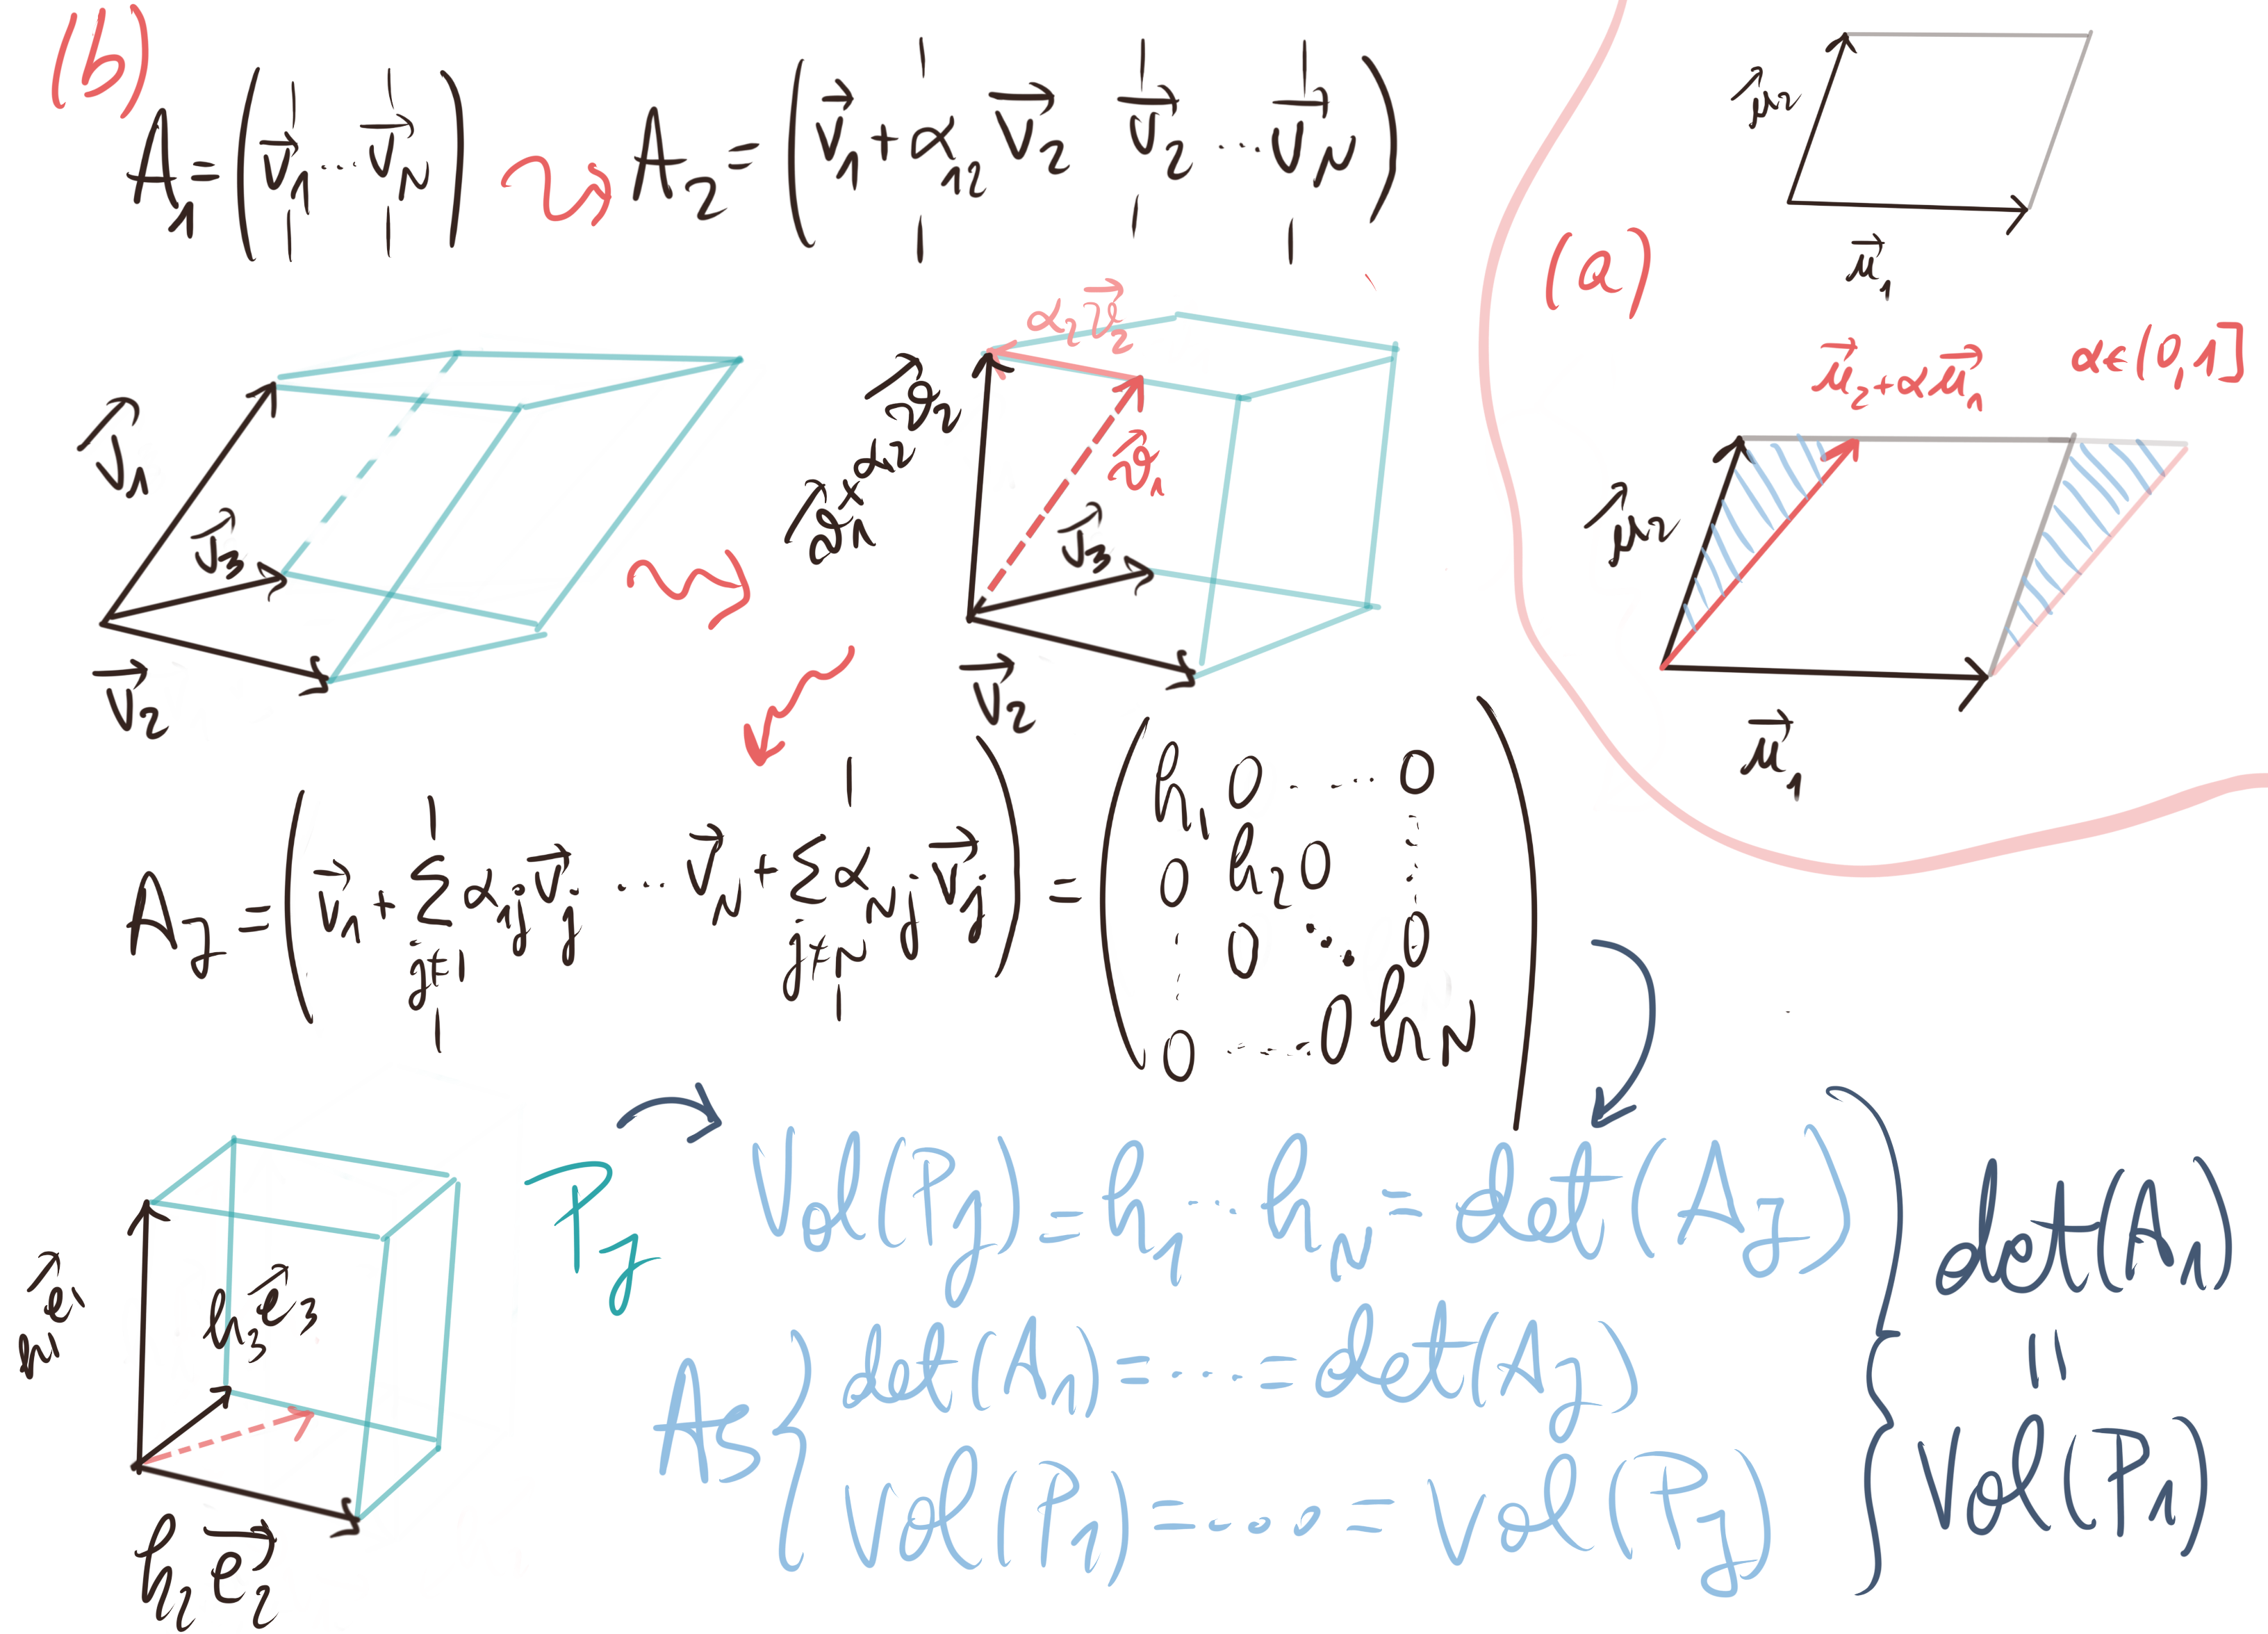
\includegraphics[width=0.65\linewidth]{10parallelepipid.png}
  \caption{ {\bf (a)} A visual proof that a parallelogram does not change its area if we take any of the vectors delimiting its edges, multiply it by any real $\alpha>0$ and sum it to the other vector. If $\alpha\in(0,1]$, as it can be seen in the drawing, we can identify the area of the new parallelogram that is not over the old parallelogram to be the area of the old that is not under the new one (blue). Thus their areas must be the same. For any $\alpha>1$, we could find some $\beta_i\in(0,1]$ such that $\alpha=\sum_i\beta_i$, and apply recursively the rule that the area does not change for each of the additions, relative to the previous parallelogram. The proof then is also valid for any parallelepiped, since its faces are parallelograms; to any 4-parallelotope since its 4-faces are parallelepipeds and so on, to any $N$-parallelotope.\\ {\bf (b)} Heuristic algebraic/geometric argument following the written heuristic proof. \vspace{-0.4cm} }
  \label{fig:volumeDet}
\end{figure}

Now, regard a matrix as a linear application sending the canonical unit vectors to its column vectors. Then, since the volume of the canonical unit vector cube is 1, the determinant of the matrix, the volume of the parallelotope in which we transform the unit cube, must be the factor by which the $N$-volume is scaled by the linear transformation. Therefore, the determinant of the Jacobian matrix of the trajectories of the fluid elements $\vec{x}(\vec{\xi},t)$, will give in magnitude, the local factor by which the volume between nearby fluid elements is scaled (dilated or contracted). Let us denote this quantity as the {\bf Jacobian determinant}: \vspace{-0.3cm}
\begin{equation}
J(\vec{\xi},t):=|det (D_\xi \vec{x}(\vec{\xi},t))|>0 \vspace{-0.1cm}
\end{equation}
If $J(\vec{\xi},t)>1$, in the locality of $\vec{\xi}$, the fluid is dilated. This means that given a fluid element labelled $\vec{\xi}^*$, the fluid elements that were closest to it at the time we made the labels: those in the ball $\{\vec{\xi}\in\Omega_0:||\vec{\xi}^*-\vec{\xi}||=\varepsilon\}$ for a small enough $\varepsilon>0$, are now getting further in configuration-space: $||\vec{x}(\vec{\xi}_0,t)-\vec{x}(\vec{\xi}_1,t)||>\varepsilon$ for this $t>t_0$. Conversely, if $J(\vec{\xi},t)<1$, the distance will get smaller.

\subsection*{ The Change of Variables in an Integral\vspace{-0.2cm}}
This interpretation of the Jacobian is why it is used in the variable changes of integrals. Say we wish to compute the $N$-volume in configuration-space that occupy at time $t$ the fluid elements that at $t_0$ were in the domain $\Omega_0$. They will now be in a domain $\Omega_t=\vec{x}(\Omega_0,t)$, so we seek the integral: $\iint_{\vec{x}(\Omega,t)}dx_1\cdots dx_N$. If we discretize the space around the point $\vec{\xi}$, in the limit of small discrete steps $\Delta x_j, \Delta \xi_j \rightarrow 0$, we will have for each point $\vec{\xi}$ that $\Delta x_1\cdots \Delta x_N= J(\vec{\xi},t)\Delta \xi_1\cdots \Delta\xi_N$, since the Jacobian gives the volume increase factor in the immediate neighbourhood of the point. If we made a continuous sum of these elements over all the volume $\Omega_0$ in label space, by the definition of the integral as the limit of Riemann sums, we would find the volume we were looking for to be:
\begin{equation}\label{volume}
\iint_{\vec{x}(\Omega,t)}dx_1\cdots dx_N=\iint_{\Omega} J(\vec{\xi},t) d\xi_1\cdots d\xi_N
\end{equation}
More formally, since $\forall \vec{\xi}\in B_\varepsilon(\vec{\xi}^*)$ with $\varepsilon\rightarrow 0$ we have that $\vec{x}(\vec{\xi},t)-\vec{x}(\vec{\xi}^*,t)= D_{\vec{\xi}}\vec{x}(\vec{\xi}^*,t)\cdot (\vec{\xi}-\vec{\xi}^*)$, then for $\varepsilon \rightarrow 0$:
\begin{equation}
Vol\qty(\vec{x}(\Omega,t)\cap B_\varepsilon(\vec{x}(\vec{\xi},t)))=J(\vec{\xi},t)Vol\qty(\Omega \cap B_\varepsilon (\vec{\xi}))
\end{equation}
\begin{equation}
Vol\qty(\vec{x}(\Omega))=\lim_{ \varepsilon\rightarrow 0} \sum_{\vec{\xi}\in\Omega} Vol\qty(\vec{x}(\Omega,t)\cap B_\varepsilon(\vec{x}(\vec{\xi},t)))=\lim_{ \varepsilon\rightarrow 0} \sum_{\vec{\xi}\in\Omega} J(\vec{\xi},t)Vol\qty(\Omega \cap B_\varepsilon (\vec{\xi}))
\end{equation}
with $B_\varepsilon(x)\subset \R^N$ a ball of center $x\in\R^N$ and radious $\varepsilon>0$. Using the definition of integral, this last equation leads to equation \eqref{volume}.

More in general, if what we wanted was a weighted sum of the volume elements, where each element in configuration space has a scalar value $f(\vec{x},t)$, then we would have enough in the preceding development with multiplying each volume contribution by the value of its corresponding scalar. This would yield:
\begin{equation}\label{integralChange}
\iint_{\vec{x}(\Omega,t)}f(\vec{x},t)dx_1\cdots dx_N=\iint_{\Omega} f(\vec{x},t)\Big\rvert_{\vec{x}(\vec{\xi},t)}J(\vec{\xi},t) d\xi_1\cdots d\xi_N \vspace{-0.2cm}
\end{equation}

\subsection*{ The Inverse Transformation and its Jacobian\vspace{-0.2cm}}
Note that all of this development is equally valid for the inverse transformation, that gives the label of the trajectory that passes from each configuration space point at each time $\vec{\xi}(\vec{x},t)$. It turns out there is a very convenient connection: the Jacobian matrix of $\vec{\xi}(\vec{x},t)$ is the inverse of the Jacobian of $\vec{x}(\vec{\xi},t)$. Since one is the inverse map of the other this could have already been suspected. A more formal prove however comes from the following: since we impose that $\vec{x}(\vec{\xi}(\vec{x},t),t)=\vec{x}$, taking each $k$-th component of the vectors and derivating them by $x_j$ we get applying the chain rule that: \vspace{-0.1cm}
\begin{equation}
\pdv{}{x_j}x_k(\vec{\xi}(\vec{x},t),t)=\pdv{}{x_j}x_k \Rightarrow \sum_{l=1}^N \pdv{x_k(\vec{\xi},t)}{\xi_l}\Big\rvert_{\vec{\xi}(\vec{x},t)}\pdv{\xi_l(\vec{x},t)}{x_j}=\delta_{jk} \vspace{-0.2cm}
\end{equation}
which can be written in matrix form as:
\begin{equation}\label{inverse}
\begin{pmatrix}
\pdv{x_1}{\xi_1}&\cdots&\pdv{x_1}{\xi_N} \\
\vdots &\ddots& \vdots \\
\pdv{x_N}{\xi_1}&\cdots&\pdv{x_N}{\xi_N}
\end{pmatrix}\cdot \begin{pmatrix}
\pdv{\xi_1}{x_1}&\cdots&\pdv{\xi_1}{x_N} \\
\vdots & \ddots & \vdots \\
\pdv{\xi_N}{x_1}&\cdots&\pdv{\xi_N}{x_N}
\end{pmatrix}=\begin{pmatrix}
1&\cdots &0 \\
\vdots & 1& \vdots \\
0&\cdots &1
\end{pmatrix}\Rightarrow
\end{equation}
$$
\Rightarrow D_\xi \vec{x}(\vec{\xi},t)\cdot D_x \vec{\xi}(\vec{x},t) = Id_{NxN}
$$
Which means by the uniqueness of the inverse matrix that the Jacobian matrix of $\xi(\vec{x},t)$ is the inverse of the Jacobian matrix of $x(\xi,t)$. Namely, $D_x \vec{\xi}(\vec{x},t)=D_\xi \vec{x}(\vec{\xi},t)^{-1}$.

In particular this means that in order to compute the determinant of any of them it is enough to compute the determinant for the other one, since for any invertible matrix $A$ with inverse $A^{-1}$ we have that $det(A)=1/det(A^{-1})$. This will be relevant, because computing $D_\xi \vec{x}(\vec{\xi},t)$ will be easy at all times if we choose the label space to be a regular discretized grid, while $D_x \vec{\xi}(\vec{x},t)$ will hardly ever be so.

\subsection*{Deriving the Continuity Equation from a simple Assumption \vspace{-0.2cm} }
Let us see how useful the Jacobian is, in that we will be able to derive the continuity equation of a fluid from simple considerations. We will arrive at equation \eqref{JacPre.Bohm} by identifying a vital relationship between the velocity field driving the fluid elements and the Jacobian. In fact, we will arrive to find which is the conserved quantity along any given Bohmian trajectory, which leads to an alternative way to compute the time evolution of the density.

For this, let us first see what the continuity equation in the Eulerian frame \eqref{CE} is telling us, so that we can then derive it in the converse way. Integrating both sides of the equation on a bounded configuration space volume $V\subset\R^N$, with boundary $\partial V$, applying the divergence theorem we get:
\begin{equation}
\pdv{}{t} \int_{V} \rho(\vec{x},t) dx_1\cdots dx_N=-\int_{\partial V} \rho(\vec{x},t)\vec{v}(\vec{x},t)\cdot d\vec{S}(\vec{x})=-\int_{\partial V} \rho(\vec{x},t)v_{normal}(\vec{x},t)\cdot dS
\end{equation}
The quantity in the left-hand side is the variation in time of the amount of Universes/Bohmian-trajectories inside the configuration space volume $V$ (in units of fluid-elements/time). The one in the right is the outward flux of Universes/Bohmian-trajectories across the surface (in fluid-elements/time). Thus, the continuity equation is equivalent to imposing that there is no source or sink for the number of Universes. The variation of its number can only be due to their displacement to adjacent points of space. Universes cannot be destroyed nor created.

Now, let us derive the continuity equation in the converse way: we impose that the amount of Universes in any initial configuration space $N$-volume $V_0\subseteq\Omega_0\subseteq\R^N$, should be the same as the amount of Universes in the volume at which those Universes extend at time $t$: $\vec{x}(V_0,t)$. Mathematically this conservation of fluid-elements would mean:
\begin{equation}
\iint_{V_0} \rho(\vec{\xi},t=t_0) d\xi_1\cdots d\xi_N=\iint_{\vec{x}(V_0,t)} \rho(\vec{x},t) dx_1\cdots dx_N\quad \forall t
\end{equation}
If we use equation \eqref{integralChange} we can rewrite it as:
\begin{equation}
\iint_{V_0} \rho(\vec{\xi},t=t_0) d\xi_1\cdots d\xi_N=\iint_{V_0} \rho(\vec{\xi},t) J(\vec{\xi},t) d\xi_1\cdots d\xi_N \quad \forall t
\end{equation}
And manipulate it to get:
\begin{equation}
\iint_{V_0} \qty[ \rho(\vec{\xi},t=t_0) -\rho(\vec{\xi},t) J(\vec{\xi},t) ]d\xi_1\cdots d\xi_N=0
\end{equation}
Since this must be true for any possible $V_0$, it must be that:
\begin{equation}
\rho(\vec{\xi},t_0) = \rho(\vec{\xi},t) J(\vec{\xi},t)\Longleftrightarrow \rho(\vec{\xi},t)=\frac{\rho(\vec{\xi},t_0)}{J(\vec{\xi},t)}\Longleftrightarrow \frac{\rho(\vec{\xi},t_0)}{\rho(\vec{\xi},t)}=J(\vec{\xi},t)
\end{equation}
Or equivalently if we evaluate $\vec{\xi}=\vec{\xi}(\vec{x},t)$:
\begin{equation}
\rho(\vec{x},t_0) = \rho(\vec{x},t) J(\vec{x},t)\Longleftrightarrow \rho(\vec{x},t)=\frac{\rho(\vec{\xi},t_0)}{J(\vec{x},t)}\Longleftrightarrow \frac{\rho(\vec{x},t_0)}{\rho(\vec{x},t)}=J(\vec{x},t)
\end{equation}
On the one hand, this gives us a way to compute the density in any time by just knowing the density at the initial time $\rho(\vec{\xi},t_0)$ and $\vec{x}(\vec{\xi},t)$, since this last lets us compute the derivatives $\pdv{x_k}{\xi_j}$ and thus the Jacobian determinant $J$. On the other hand, it lets us interpret the Jacobian in fluid terms: $J(\vec{\xi},t)=\frac{\rho(\vec{\xi},t_0)}{\rho(\vec{\xi},t)}$. The Jacobian determinant of $\vec	{x}(\vec{\xi},t)$ is the (positive) ratio of the density perceived by the fluid element $\vec{\xi}$ in its local surrounding relative to the one perceived at the beginning. This can be smaller than one or greater than one. If the ratio is greater than one, then $\rho(\vec{\xi},t_0)>\rho(\vec{\xi},t)$, meaning that the fluid of configuration-space "Universes" has been diluted around $\vec{\xi}$, the density has been decreased, which is in accordance with the fact that a positive Jacobian meant the trajectories in that locality get more spaced between them. If on the other hand the ratio is smaller than one, then $\rho(\vec{\xi},t_0)>\rho(\vec{\xi},t)$, the density gets concentrated locally, in accordance with the convergence of trajectories in the surrounding. Note though that there is no source of Universes, since the Jacobian, accounting only for the movement of trajectories, is the only factor influencing the density change. This is precisely what we imposed with the integral above.

Now, let us finish deriving from here the continuity equation in the shape we get from the Schrödinger Equation. Let us take $\rho(\vec{\xi},t_0) = \rho(\vec{\xi},t) J(\vec{\xi},t)$ and derivate it at each side in time. Since the left hand side is time independent, we get:
\begin{equation}
0=\pdv{}{t}\qty( \rho(\vec{\xi},t) J(\vec{\xi},t))
\end{equation}
which implies that along any given Bohmian trajectory $\vec{\xi}$, the quantity $\rho(\vec{\xi},t) J(\vec{\xi},t)$ is a constant of motion! Further expanding the expression we get:
\begin{equation}\label{Jacobproc0}
J(\vec{\xi},t)\pdv{\rho(\vec{\xi},t)}{t}+\rho(\vec{\xi},t)\pdv{J(\vec{\xi},t)}{t}=0
\end{equation}
Then note that:
\begin{equation}\label{jainkoa}
\pdv{}{t}J(\vec{\xi},t)=J(\vec{\xi},t)\vec{\nabla}_x\cdot\vec{v}(\vec{x},t)\Big\rvert_{\vec{x}(\vec{\xi},t)}
\end{equation}
We will prove this, in the following gray box, after we get to the Continuity Equation, to avoid loosing the objective. By evaluating this identity in equation \eqref{Jacobproc0} we get:
\begin{equation}
J(\vec{\xi},t)\qty(\pdv{\rho(\vec{\xi},t)}{t}+\rho(\vec{\xi},t)\vec{\nabla}_x\cdot\vec{v}(\vec{x},t)\Big\rvert_{\vec{x}(\vec{\xi},t)})=0
\end{equation}
Since we assumed that the Jacobian of the trajectories was never zero to allow its invertibility, we will have that the differential equation multiplying it in the last equation, must be zero:
\begin{equation}
\pdv{\rho(\vec{\xi},t)}{t}+\rho(\vec{\xi},t)\vec{\nabla}_x\cdot\vec{v}(\vec{x},t)\Big\rvert_{\vec{x}(\vec{\xi},t)}=0
\end{equation}
which is the Continuity Equation in the Lagrangian frame \eqref{CE.L.Bohm}. If we now evaluate $\vec{\xi}=\vec{\xi}(\vec{x},t)$ and note:
\begin{equation}
\hspace*{-0.6cm}\pdv{\rho(\vec{\xi},t)}{t}\Big\rvert_{\vec{\xi}(\vec{x},t)}=\dv{\rho(\vec{x}(\vec{\xi},t),t)}{t}\Big\rvert_{\vec{\xi}(\vec{x},t)}=\pdv{\rho(\vec{x},t)}{t}+\sum_{k=1}^N\pdv{\rho(\vec{x},t)}{x_k}\pdv{x_k(\vec{\xi},t)}{t}\Big\rvert_{\vec{\xi}(\vec{x},t)}=\pdv{\rho(\vec{x},t)}{t}+\sum_{k=1}^N\pdv{\rho(\vec{x},t)}{x_k}v_k(\vec{x},t)
\end{equation}
We have that:
\begin{equation}
\pdv{\rho(\vec{x},t)}{t}+\sum_{k=1}^N\pdv{\rho(\vec{x},t)}{x_k}v_k(\vec{x},t)+\rho(\vec{x},t)\pdv{v_k(\vec{x},t)}{x_k}=0
\end{equation}
which reverting the derivative of a product, yields the Continuity Equation in the Eulerian frame \eqref{CE}.\vspace{0.1cm}
\mybox{
\subsection*{ What is $\pdv{}{t}J(\vec{\xi},t)$?\vspace{-0.1cm}}
Let us prove the identity \eqref{jainkoa}, since it has its very big relevance. For this, we can start from the definition of determinant in all of its glory:
\begin{equation}
J(\vec{\xi},t)=\qty|det \Big( D_\xi \vec{x}(\vec{\xi},t) \Big)|=\sum_p sgn(p) \pdv{x_1}{\xi_{p1}} \cdots \pdv{x_N}{\xi_{pN}}
\end{equation}
with the sum running over all the $N!$ possible permutation tuples $p=(p_1,...,p_N)$ for $\{1,...,N\}$ and $sgn(p)$ the sign of the permutation. Then, using the Leibniz derivation rule for products:}
\mybox{
\begin{equation}\label{Jacobproc}
\pdv{}{t}J(\vec{\xi},t)=\sum_p sgn(p) \Bigg(\qty[\pdv{}{t}\pdv{x_1}{\xi_{p1}}]\pdv{x_2}{\xi_{p2}} \cdots \pdv{x_N}{\xi_{pN}}+\pdv{x_1}{\xi_{p1}}\qty[\pdv{}{t}\pdv{x_2}{\xi_{p2}}] \cdots \pdv{x_N}{\xi_{pN}}+\cdots
\end{equation}
$$
+\pdv{x_1}{\xi_{p1}} \cdots \pdv{x_{N-1}}{\xi_{pN-1}}\qty[\pdv{}{t}\pdv{x_N}{\xi_{pN}}]\Bigg)
$$
Note that since $\pdv{x_j(\vec{\xi},t)}{t}=:v_j(\vec{\xi},t)=v_k(\vec{x}(\vec{\xi},t),t)$:
\begin{equation}
\pdv{}{t}\pdv{x_i(\vec{\xi},t)}{\xi_j}=\pdv{}{\xi_j}\pdv{x_i(\vec{\xi},t)}{t}=\pdv{}{\xi_j}v_i(\vec{x}(\vec{\xi},t),t)=\sum_{k=1}^N \pdv{v_i(\vec{x},t)}{x_k}\Big\rvert_{\vec{x}(\vec{\xi},t)}\pdv{x_k(\vec{\xi},t)}{\xi_j}
\end{equation}
This leaves equation \eqref{Jacobproc} as:
\begin{equation}
\pdv{}{t}J(\vec{\xi},t)=\sum_p sgn(p) \Bigg(\qty[\sum_{k=1}^N \pdv{v_1(\vec{x},t)}{x_k}\Big\rvert_{\vec{x}(\vec{\xi},t)}\pdv{x_k(\vec{\xi},t)}{\xi_{p1}}]\pdv{x_2}{\xi_{p2}} \cdots \pdv{x_N}{\xi_{pN}}+\cdots
\end{equation}
$$
+\pdv{x_1}{\xi_{p1}} \cdots \pdv{x_{N-1}}{\xi_{pN-1}}\qty[\sum_{k=1}^N \pdv{v_N(\vec{x},t)}{x_k}\Big\rvert_{\vec{x}(\vec{\xi},t)}\pdv{x_k(\vec{\xi},t)}{\xi_{pN}}]\Bigg)=
$$
$$
=\sum_{k=1}^N\sum_p sgn(p) \pdv{v_1(\vec{x},t)}{x_k}\Big\rvert_{\vec{x}(\vec{\xi},t)}\pdv{x_k(\vec{\xi},t)}{\xi_{p1}}\pdv{x_2}{\xi_{p2}} \cdots \pdv{x_N}{\xi_{pN}}+\cdots 
$$
$$
+ \sum_{k=1}^N\sum_p sgn(p)\pdv{x_1}{\xi_{p1}} \cdots \pdv{x_{N-1}}{\xi_{pN-1}}\pdv{v_N(\vec{x},t)}{x_k}\Big\rvert_{\vec{x}(\vec{\xi},t)}\pdv{x_k(\vec{\xi},t)}{\xi_{pN}}=
$$
$$
=\sum_{k=1}^N \pdv{v_1(\vec{x},t)}{x_k}\Big\rvert_{\vec{x}(\vec{\xi},t)}\sum_p sgn(p)\pdv{x_k}{\xi_{p1}}\pdv{x_2}{\xi_{p2}} \cdots \pdv{x_N}{\xi_{pN}}+\cdots 
$$
$$
+ \sum_{k=1}^N\pdv{v_N(\vec{x},t)}{x_k}\Big\rvert_{\vec{x}(\vec{\xi},t)}\sum_p sgn(p)\pdv{x_1}{\xi_{p1}} \cdots \pdv{x_{N-1}}{\xi_{pN-1}}\pdv{x_k}{\xi_{pN}}
$$
where recalling the definition of determinant, we can see that it is a sum of many determinants, many of which will be zero since they will have rows with the same elements (thus the $N$-volume of the parallelotopes that form their rows will be null). We can see clearly from the last equation that:
\begin{equation}
\pdv{}{t}J(\vec{\xi},t)=\sum_{k=1}^N \pdv{v_1(\vec{x},t)}{x_k}\Big\rvert_{\vec{x}(\vec{\xi},t)} \begin{vmatrix}
\pdv{x_k}{\xi_{1}}&\pdv{x_k}{\xi_{2}} &\cdots &\pdv{x_k}{\xi_{N}}\\
\pdv{x_2}{\xi_{1}}&\pdv{x_2}{\xi_{2}} &\cdots &\pdv{x_2}{\xi_{N}}\\
\vdots & \ddots & \vdots\\
\pdv{x_N}{\xi_{1}}&\pdv{x_N}{\xi_{2}} &\cdots &\pdv{x_N}{\xi_{N}}
\end{vmatrix}+\cdots+
\pdv{v_N(\vec{x},t)}{x_k}\Big\rvert_{\vec{x}(\vec{\xi},t)} \begin{vmatrix}
\pdv{x_1}{\xi_{1}}&\pdv{x_1}{\xi_{2}} &\cdots &\pdv{x_1}{\xi_{N}}\\
\pdv{x_2}{\xi_{1}}&\pdv{x_2}{\xi_{2}} &\cdots &\pdv{x_2}{\xi_{N}}\\
\vdots & \ddots & \vdots\\
\pdv{x_k}{\xi_{1}}&\pdv{x_k}{\xi_{2}} &\cdots &\pdv{x_k}{\xi_{N}}
\end{vmatrix}
\end{equation}
In each determinant, if the index $k$ is in row $j$, for all the $k\neq j$, the determinant will have two equal rows, leaving only those determinants with $k=j$, which turn out to be the Jacobian matrix determinants! Thus, we can take them as common factors to get that:
\begin{equation}
\pdv{}{t}J(\vec{\xi},t)=\qty(\pdv{v_1(\vec{x},t)}{x_k}\Big\rvert_{\vec{x}(\vec{\xi},t)}+\cdots+\pdv{v_N(\vec{x},t)}{x_k}\Big\rvert_{\vec{x}(\vec{\xi},t)}) J(\vec{\xi},t))\Leftrightarrow
\end{equation}
\begin{equation}\label{EulerDif}
\pdv{}{t}J(\vec{\xi},t)=J(\vec{\xi},t)\vec{\nabla}_x\cdot\vec{v}(\vec{x},t)\Big\rvert_{\vec{x}(\vec{\xi},t)}
\end{equation}
which is what we wanted to prove. $o.\varepsilon.\delta$.}
\mybox{
Equation \eqref{EulerDif} is a differential equation stating how the Jacobian of a certain fluid element evolves in time, given we know the velocity field moving those fluid elements. In particular, this means that:\vspace{-0.2cm}
\begin{equation}
J(\vec{\xi},t)=J(\vec{\xi},t_0)e^{\int_{t0}^t \vec{\nabla}_x\cdot\vec{v}(\vec{x},t)\Big\rvert_{\vec{x}(\vec{\xi},t)}dt}
\end{equation}
where as $J(\vec{\xi},t_0)=1$ by definition, we have that:\vspace{-0.2cm}
\begin{equation}
\frac{1}{J(\vec{\xi},t)}=\frac{\rho(\vec{\xi},t)}{\rho(\vec{\xi},t_0)}=e^{-\int_{t0}^t \vec{\nabla}_x\cdot\vec{v}(\vec{x},t)\Big\rvert_{\vec{x}(\vec{\xi},t)}dt}
\end{equation}
which is the propagator equation we found in equation \eqref{JacPre.Bohm} from the continuity equation in the Lagrangian frame. This equation has a very big relevance, since it allows the computation of the Jacobian, the density and the Bohmian velocity field, just by knowing two of them. Also, it is the expression where all the interpretations we were dealing with are summarized.}

\section*{(II.e) Partial Derivatives relative to the Labels}
\addcontentsline{toc}{subsubsection}{{\bf (II.e)} Partial Derivatives relative to the Labels}
As we already commented in (II.a), one of the main problems with the Lagrangian frame is that the fluid-elements move in directions that end up unstructuring the initial mesh, which could have been a regular Cartesian mesh at the beginning, but will not in the next time iterations. To solve this, what we could do is to convert the partial derivatives in the configuration-space Eulerian positions $x_k$ into partial derivatives in the label configuration-space positions $\xi_j$, using the fact that since we are evolving trajectories we have knowledge of the function $\vec{x}(\vec{\xi},t)$. As an example, lets analyse how we could compute $\pdv{f(\vec{x},t)}{x_k}\Big\rvert_{\vec{x}(\vec{\xi},t)}$. By the chain rule:
\begin{equation}
\pdv{f(\vec{x},t)}{x_k}=\dv{f(\vec{\xi}(\vec{x},t),t)}{x_k}=\sum_{j=1}^N \pdv{f(\vec{\xi},t)}{\xi_j}\Big\rvert_{\vec{\xi}(\vec{x},t)} \pdv{\xi_j(\vec{x},t)}{x_k}
\end{equation}
which can be evaluated at $\vec{x}=\vec{x}(\vec{\xi},t)$ to get:
\begin{equation}
\pdv{f(\vec{x},t)}{x_k}\Big\rvert_{\vec{x}(\vec{\xi},t)}=\sum_{j=1}^N \pdv{f(\vec{\xi},t)}{\xi_j} \pdv{\xi_j(\vec{x},t)}{x_k}\Big\rvert_{\vec{x}(\vec{\xi},t)}
\end{equation}
We see that we can freely change the derivative in $x_k$ by derivatives in $\xi_j$, as long as we also know how to compute $\pdv{\xi_j(\vec{x},t)}{x_k}$, which are the elements of the Jacobian matrix of $\vec{\xi}(\vec{x},t)$. If we attempt to directly compute them, we immediately acknowledge that these derivatives are still in an unstructured grid. However, as we proved in equation \eqref{inverse}, we have that the Jacobian matrix $D_x \vec{\xi}(\vec{x},t)$ where the element in row $j$ and column $k$ is $\pdv{\xi_j(\vec{x},t)}{x_k}$, is the inverse of the Jacobian matrix $D_\xi \vec{x}(\vec{\xi},t)$, the entries of which are of the shape $\pdv{x_j(\vec{\xi},t)}{\xi_k}$. Observe that the entries of this last Jacobian matrix can actually be computed in a regular grid if we chose the label space to be so, by just knowing the trajectories of the fluid elements! Therefore, if we first compute the elements $\pdv{x_j(\vec{\xi},t)}{\xi_k}$ of the matrix $D_\xi \vec{x}(\vec{\xi},t)$ and then compute the inverse matrix with any possible method, we will have computed the values $\pdv{\xi_j(\vec{x},t)}{x_k}$ in a structured grid.

A possible way to compute the entries of the inverse matrix would be by using the inverse matrix theorem. This theorem can be summarized as follows. Let $A$ be an $N\cross N$ invertible (non-singular) matrix. Then:
\begin{itemize}
\item Its $i,j$ {\bf minor}, which we will note by $Min(A)_{ij}$, is the $(N-1)\cross (N-1)$ matrix obtained by deleting row $i$ and column $j$.
\item Its $i,j$ {\bf cofactor}, which we will note by $Cof(A)_{ij}$, is: $(-1)^{i+j}det\qty(Min(A)_{ij})$.
\item Its inverse matrix is then:
\begin{equation}
A^{-1}=\frac{1}{det(A)} \begin{pmatrix}
Cof(A)_{11} & Cof(A)_{21}&\cdots& Cof(A)_{N1}\\
Cof(A)_{12} & Cof(A)_{22}&\cdots& Cof(A)_{N2}\\
\vdots & \vdots & \ddots & \vdots \\
Cof(A)_{1N} & Cof(A)_{2N}&\cdots& Cof(A)_{NN}\\
\end{pmatrix}
\end{equation}
Thus, if we denote the $i,j$ element of $A^{-1}$ as $(A^{-1})_{ij}$, we have that:
\begin{equation}
(A^{-1})_{ij} = (-1)^{j+i}\ det\qty(Min(A)_{ji} )
\end{equation}
\end{itemize}
Therefore, we have that:
\begin{equation}\label{JacobChange}
\pdv{\xi_i(\vec{x},t)}{x_j}\Big\rvert_{\vec{x}(\vec{\xi},t)} = \frac{ (-1)^{i+j}}{det \qty(D_{\xi} \vec{x}(\vec{\xi},t))}\cdot det \qty(D_{\xi} \vec{x}(\vec{\xi},t)\textit{ erasing the row and column of }\pdv{x_j(\vec{\xi},t)}{\xi_i} )
\end{equation}
For example in $N=1$ this means that:
\begin{equation}
\pdv{\xi(\vec{x},t)}{x}\Big\rvert_{\vec{x}(\vec{\xi},t)}=\frac{1}{\pdv{x(\xi,t)}{\xi}}
\end{equation}
In $N=2$:
\begin{equation}
\begin{pmatrix}
\pdv{\xi_1}{x_1} & \pdv{\xi_1}{x_2} \vspace{0.15cm}\\
\pdv{\xi_2}{x_1} & \pdv{\xi_1}{x_2}
\end{pmatrix}\Big\rvert_{\vec{x}(\vec{\xi},t)}= \frac{1}{J} \begin{pmatrix}
\pdv{x_2}{\xi_2} & - \pdv{x_1}{\xi_2} \vspace{0.15cm}\\
-\pdv{x_2}{\xi_1} & \pdv{x_1}{\xi_1
} 
\end{pmatrix}
\end{equation}
In $N=3$:
\begin{equation}
\begin{pmatrix}
\pdv{\xi_1}{x_1} & \pdv{\xi_1}{x_2} & \pdv{\xi_1}{x_3} \vspace{0.15cm}\\
\pdv{\xi_2}{x_1} & \pdv{\xi_1}{x_2} & \pdv{\xi_2}{\xi_3}\vspace{0.15cm}\\
\pdv{\xi_3}{x_1} & \pdv{\xi_3}{x_2} & \pdv{\xi_3}{\xi_3}
\end{pmatrix}\Big\rvert_{\vec{x}(\vec{\xi},t)}= \frac{1}{J} \begin{pmatrix}
\pdv{x_2}{\xi_2}\pdv{x_3}{\xi_3}-\pdv{x_2}{\xi_3}\pdv{x_3}{\xi_2} & \pdv{x_1}{\xi_3}\pdv{x_3}{\xi_2}- \pdv{x_1}{\xi_2}\pdv{x_3}{\xi_3} & \pdv{x_1}{\xi_2}\pdv{x_2}{\xi_3}-\pdv{x_1}{\xi_3}\pdv{x_2}{\xi_2} \vspace{0.15cm}\\

\pdv{x_2}{\xi_3}\pdv{x_3}{\xi_1}-\pdv{x_2}{\xi_1}\pdv{x_3}{\xi_3} & \pdv{x_1}{\xi_1}\pdv{x_3}{\xi_3}- \pdv{x_1}{\xi_3}\pdv{x_3}{\xi_1} & \pdv{x_1}{\xi_3}\pdv{x_2}{\xi_1}-\pdv{x_1}{\xi_1}\pdv{x_2}{\xi_3} \vspace{0.15cm}\\

\pdv{x_2}{\xi_1}\pdv{x_3}{\xi_2}-\pdv{x_2}{\xi_2}\pdv{x_3}{\xi_1} & \pdv{x_1}{\xi_2}\pdv{x_3}{\xi_1}- \pdv{x_1}{\xi_1}\pdv{x_3}{\xi_2} & \pdv{x_1}{\xi_1}\pdv{x_2}{\xi_2}-\pdv{x_1}{\xi_2}\pdv{x_2}{\xi_1} \\

\end{pmatrix}
\end{equation}
where by $J$, we mean in this case, the {\bf signed} Jacobian determinant of $\vec{x}(\vec{\xi},t)$,  $J(\vec{\xi},t):=det(D_\xi\vec{x}(\vec{\xi},t))$.

Then, in any of the differential equations we develop that contain Lagrangian degrees of freedom we will be able to do the following change for the partial derivatives in Eulerian positions:
\begin{equation}
\sum_{a=1}^N \pdv{f(\vec{x},t)}{x_a}\Big\rvert_{\vec{x}(\vec{\xi},t)} = \sum_{j=1}^N \pdv{f(\vec{\xi},t)}{\xi_j} \sum_{a=1}^N \pdv{\xi_j(\vec{x},t)}{x_a}\Big\rvert_{\vec{x}(\vec{\xi},t)}
\end{equation}
where we now know how to compute all the terms. For the Laplacian we could proceed much in the same way iteratively, to get:
\begin{equation}
\sum_{a=1}^N \pdv[2]{f(\vec{x},t)}{x_a}\Big\rvert_{\vec{x}(\vec{\xi},t)}=\frac{1}{J} \sum_{j=1}^N\pdv{}{\xi_j} \qty[ J\sum_{k=1}^N\pdv{f}{\xi_k}\sum_{a=1}^N\pdv{\xi_k}{x_a}\pdv{\xi_j}{x_a}\Big\rvert_{\vec{x}(\vec{\xi},t)}]
\end{equation}
Taking into account that for each fluid element at each time we will need to compute all those partial derivatives (even if they will be in a regular grid) and the inverse of an $N\times N$ matrix, it is clear that the approach of changing the differential equations to label space is not a miracle at all. Yet, it is a possible option that can be used at least for computing some of the derivatives avoiding function fitting, which in high dimensions could be more costly than proceeding with these operations. We could still be forced to simultaneously evolve many fluid elements, but now the derivatives could be done in a regular grid. Note that we have not assumed any motion rule for the trajectories, so this is a valid approach also for the arbitrary dynamic grids we will explore in Section (II.g).


\section*{(II.g) Adaptive Grid Equations\vspace{-0.2cm}}
\addcontentsline{toc}{subsubsection}{{\bf (II.g)} Adaptive Grid Equations}

If for a moment we forget about evolving Bohmian trajectories, because we are interested on the values of the state variables $S,R$ or $\psi$ alone, we could force the fluid elements to trace custom trajectories over which we would know their values. For example, we could make them get more agglomerated around very spiky or nodal regions (which are typically avoided by Bohmian trajectories and thus get undersampled) and to run away from very smooth regions (where we are not that interested to have a big representation).

This is possible since the decision to define the velocity field for the fluid element trajectories was left open both in the Schrödinger and the Hamilton-Jacobi pictures. We said that following the analogy with classical mechanics, the derivatives of the phase $S$ were an interesting choice for the velocity fields. However, this might look quite arbitrary from the numerical standpoint. Alternatively, we could have forced the velocity field to follow any other rule as a function of the state of the wavefunction. In fact, once the fields are evolved along these custom trajectories, we can still compute Bohmian trajectories {\em a posteriori} by using the phase values of the moving mesh. \vspace{-0.1cm}

In order to avoid confusion, in this section we will use the term "mesh element" to designate fluid elements, the trajectories of which are evolved using laws other than the Bohmian one \eqref{ImpBohm}. We will reserve the term "fluid element" to designate the ones that are evolved following Bohmian trajectories. Also, instead of using the term "fluid", we will employ the terms "adaptive grid" or "moving mesh" to denote the ensemble of trajectories since these fluid elements, away from having a clear ontological nature, are just pragmatical components of a mesh that evolves in time adapting itself to the state of the system. \vspace{-0.1cm}

\hspace{-0.2cm}Let us suggest three ways in which we could proceed, inspired by the ones exposed in Reference \cite{Wyatt}.\vspace{-0.3cm}

\subsection*{\bf (II.g.1) Leave the trajectories still}\vspace{-0.2cm}
 We could directly fix $\vec{x}(t;\vec{\xi})=\vec{\xi}\ \forall t$, meaning that the velocity field for the mesh elements would be null $\pdv{}{t}\vec{x}(\vec{\xi},t)=0\ \forall t$. This would make the Advective correlation term \eqref{Adv} null, and since the grid of fluid elements would preserve its initial regularity, the approach would be identical to a fully Eulerian one. That is, solving the Lagrangian Schrödinger Equation \eqref{KinAdv} would be the same as trying to solve the Eulerian Schrödinger Equation \eqref{SE}. Perhaps an advantage of acknowledging each mesh element can be seen as an independent entity is that it could suggest a Schrödinger Equation solver that could be way more parallelizable. One could evolve the value of the quantum fields at each mesh position in parallel, then allow a cross talk to compute the partial derivatives in configuration-space and then again a parallel time step. This is why we said that in reality, fully Eulerian equations can also be parallelized if we suggest an implicit fluid-like treatment.\vspace{-0.2cm}

\subsection*{\bf (II.g.2) Make a moving mesh preserving grid spacing}\vspace{-0.2cm}
By initially defining a regular grid of mesh elements, regular in the sense that there is an equal spacing between the grid points and its boundary is an $N$-orthotope, we could allow the mesh to move with the state variable but preserving the equal spacing between the points. This would allow an efficient and straightforward computation of the spatial derivatives $\pdv{}{x_k}$ at any time. \vspace{-0.1cm}

Here is a possible implementation of this in $N=1$. At each time step, after computing the value of the state variables at each grid point:\vspace{-0.3cm}
\begin{enumerate}
\item Take the two vertices of the mesh, treat them like Bohmian trajectories and evolve them to their following position.\vspace{-0.15cm}
\item Compute an equispaced grid inside this domain with the same number of mesh points as the previous grid. Knowing the positions where the mesh points should be in the next time, compute the velocity of each old mesh point to arrive there. If for example, we are using a simple Euler method to evolve the trajectories, use: $\pdv{}{t}x(\xi,t_{j})=\frac{x(\xi,t_{j+1})-x(\xi,t_{j})}{t_{j+1}-t_j}$.
\item Compute the spatial derivatives $\pdv{}{x}$ of the quantum fields at each old grid point, using standard equispaced mesh methods.
\item Employing the computed velocity and spatial derivatives, compute the value of the state variables on each new mesh point using the time evolution equations described earlier for them.\vspace{-0.2cm}
\end{enumerate}
Note how this would allow the mesh to dynamically move wherever most of the probability density goes, avoiding the need to fix a giant grid as a fixed scenario where the wavefunction is restricted to stay. It does not only reduce the number of necessary points to map a scenario (the grid is always more or less dense wherever the wavefunction is most probable), but it also allows the mesh to avoid getting to small or too big when the wave-packet contracts or expands (Bohmian trajectories inflate or deflate). 
 
In $N>1$ the method is not as straightforward as it might seem, since the mesh looses the straight angles between the edges of the mesh domain if we allow each vertex to move as Bohmian trajectories: say, in 2D, an initial rectangle mesh will become an irregular quadrangle. This is a problem in that now there are more "grid boundaries" for the computation of partial derivatives in space and that the generation of a mesh with the same number of points inside might not be trivial. However, we could make slight modifications to the method in order to make the mesh move, contract and dilate with the probability density, but also preserve the angles at the vertices. For this, the vertices would not exactly follow the density in the Bohmian sense, but could track the expectation of the fluid. For example, the following method would preserve a regular initial $N$-hypercube grid and allow its evolution with the fluid. Once for an initial grid we compute the values of the state variables in the following time:\vspace{-0.2cm}
\begin{enumerate}
\item Numerically compute the new center of mass (the expectation) of the probability density.
\item Taking the center of mass, compute the numerical integral of the density around it in hypercubes of each time a bigger grid element width, until you find the hypercube surrounding the center of mass with, say, $99\%$ of the normalized density inside (or another custom value).
\item Define the $2^N$ corners of this hypercube as the vertices of the grid in the next time and compute the new regular grid inside it with the same number of points. Knowing the positions where the mesh points should be in the next time, compute the velocity of each old mesh point to arrive there. If for example, we are using a simple Euler method to evolve the trajectories, use: $\pdv{}{t}x_k(\xi,t_{j})=\frac{x_k(\xi,t_{j+1})-x_k(\xi,t_{j})}{t_{j+1}-t_j}$.
\begin{figure}[h!]
  \centering
    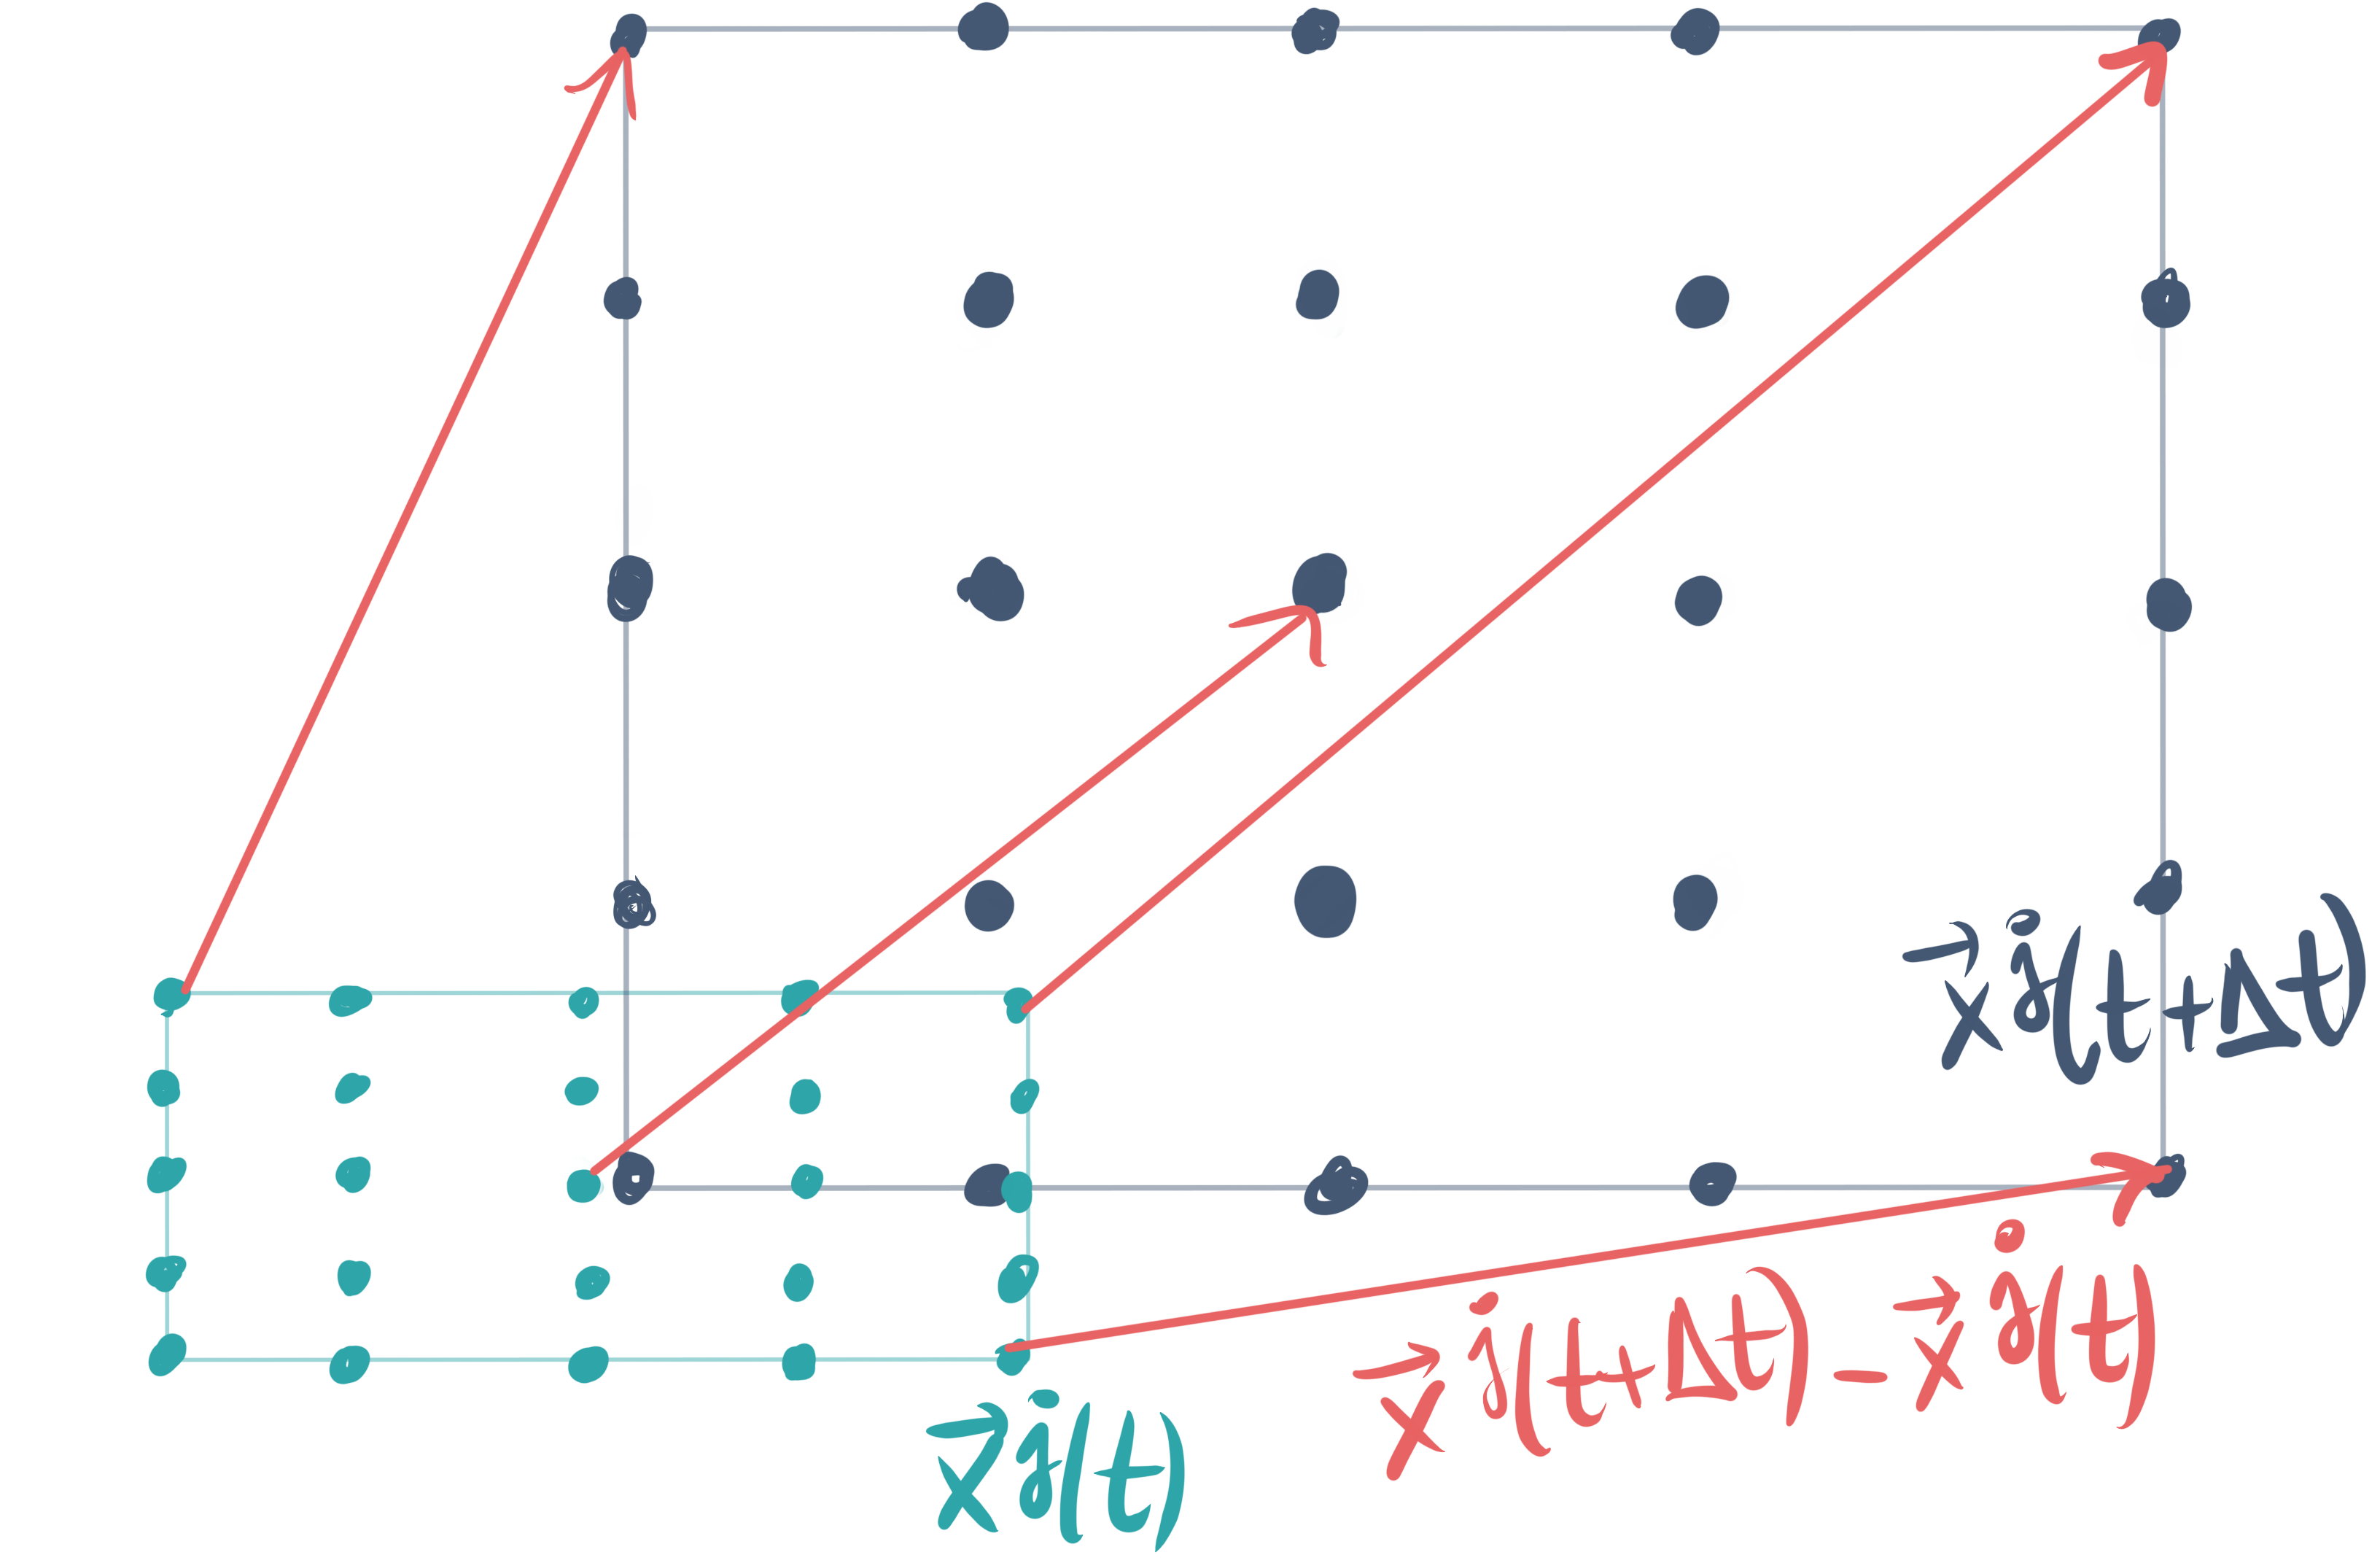
\includegraphics[width=0.45\linewidth]{9orthotope.png}
  \caption{ An intuition of how the orthotope mesh would evolve to the next time step, preserving the orthogonality of the edges of the domain but adapting itself in size (and even aspect-ratio) to the state of the evolved function. \vspace{-0.2cm}}
  \label{fig:ortho}
\end{figure}
\item Compute the spatial derivatives $\pdv{}{x_k}$ of the quantum fields at each old grid point, using standard equispaced mesh methods.
\item Employing the computed velocity and spatial derivatives, compute the value of the state variables on each new mesh point using the time evolution equations described earlier for them.
\end{enumerate}

As a side-note, if we really achieved a dynamical mesh maintaining its regularity, we would not need to use a method like the QTM. Instead we could use any regular grid method (like matrix methods) typical of the Eulerian picture, by just changing the boundary conditions at each time.

This method solves the problem of the unstructuring grid (for computing partial derivatives) that Bohmian mesh elements had, with the advantage that the grid still moves along the regions of interest. However, as we have seen, it is not as flexible as it could be.\vspace{-0.1cm}

\subsection*{\bf (II.g.3) Move the mesh using arbitrary monitor functions \vspace{-0.05cm}} 
Regions of high curvature for the action, density or the wavefunction, nodal points etc. (avoided by Bohmian trajectories), are not only interesting for their theoretical implications, but because the time evolution of the fluid elements depends on spatial derivatives in all directions, and those regions can highly influence them: if we have no representatives from those regions, we will not have enough information to allow a proper time evolution. In order to face this problem, we could force the trajectories to be attracted by regions with high curvature, among others.\vspace{-0.2cm}

\subsubsection*{(II.g.3.1) The equidistribution principle \vspace{-0.2cm}}
For doing this, a standard approach is to force the mesh elements to get into positions that equalize the integral of a positive monitor function $M(\vec{x},t)>0$ in each grid-cell: the so called {\em equidistribution principle}. In $N=1$ the intuition is immediate. It is to find at each time $t$, the grid points $\{x^j\}_{j=1}^n$ that satisfy:\vspace{-0.1cm}
\begin{equation}
\int^{x^{j+1}}_{x^j} M(x,t) dx =C \quad \forall j
\end{equation}
for a fixed constant $C$. If we discretize the integral, we get:
\begin{equation}\label{discEq}
M_j(t)\cdot (x^{j+1}-x^j)=C \quad \forall j \vspace{-0.1cm}
\end{equation}
where $M_j(t)$ could be the average of the monitor function evaluated at the edges of the grid-cell, or rather the mid-point interpolation. If for example, the monitor $M$ is chosen to be $M(x,t)=|\pdv{\rho(x,t)}{x}|$, then the bigger the curvature of the density around a grid cell, the denser the grid will become, since equation \eqref{discEq} would require a smaller step between nodes $x^j$. If on the other hand, the curvature gets flatter (and thus $M$ smaller), the grid will try to space more the nodes. See Figure \ref{fig:equid} to get a visual intuition. Note that in reality, we should choose the monitor function to be $M(x,t)=\varepsilon+|\pdv{\rho(x,t)}{x}|$ for some $\varepsilon>0$, in order to avoid an infinite separation wherever the density is exactly flat.\vspace{0.1cm}
\begin{figure}[h!]
  \centering
    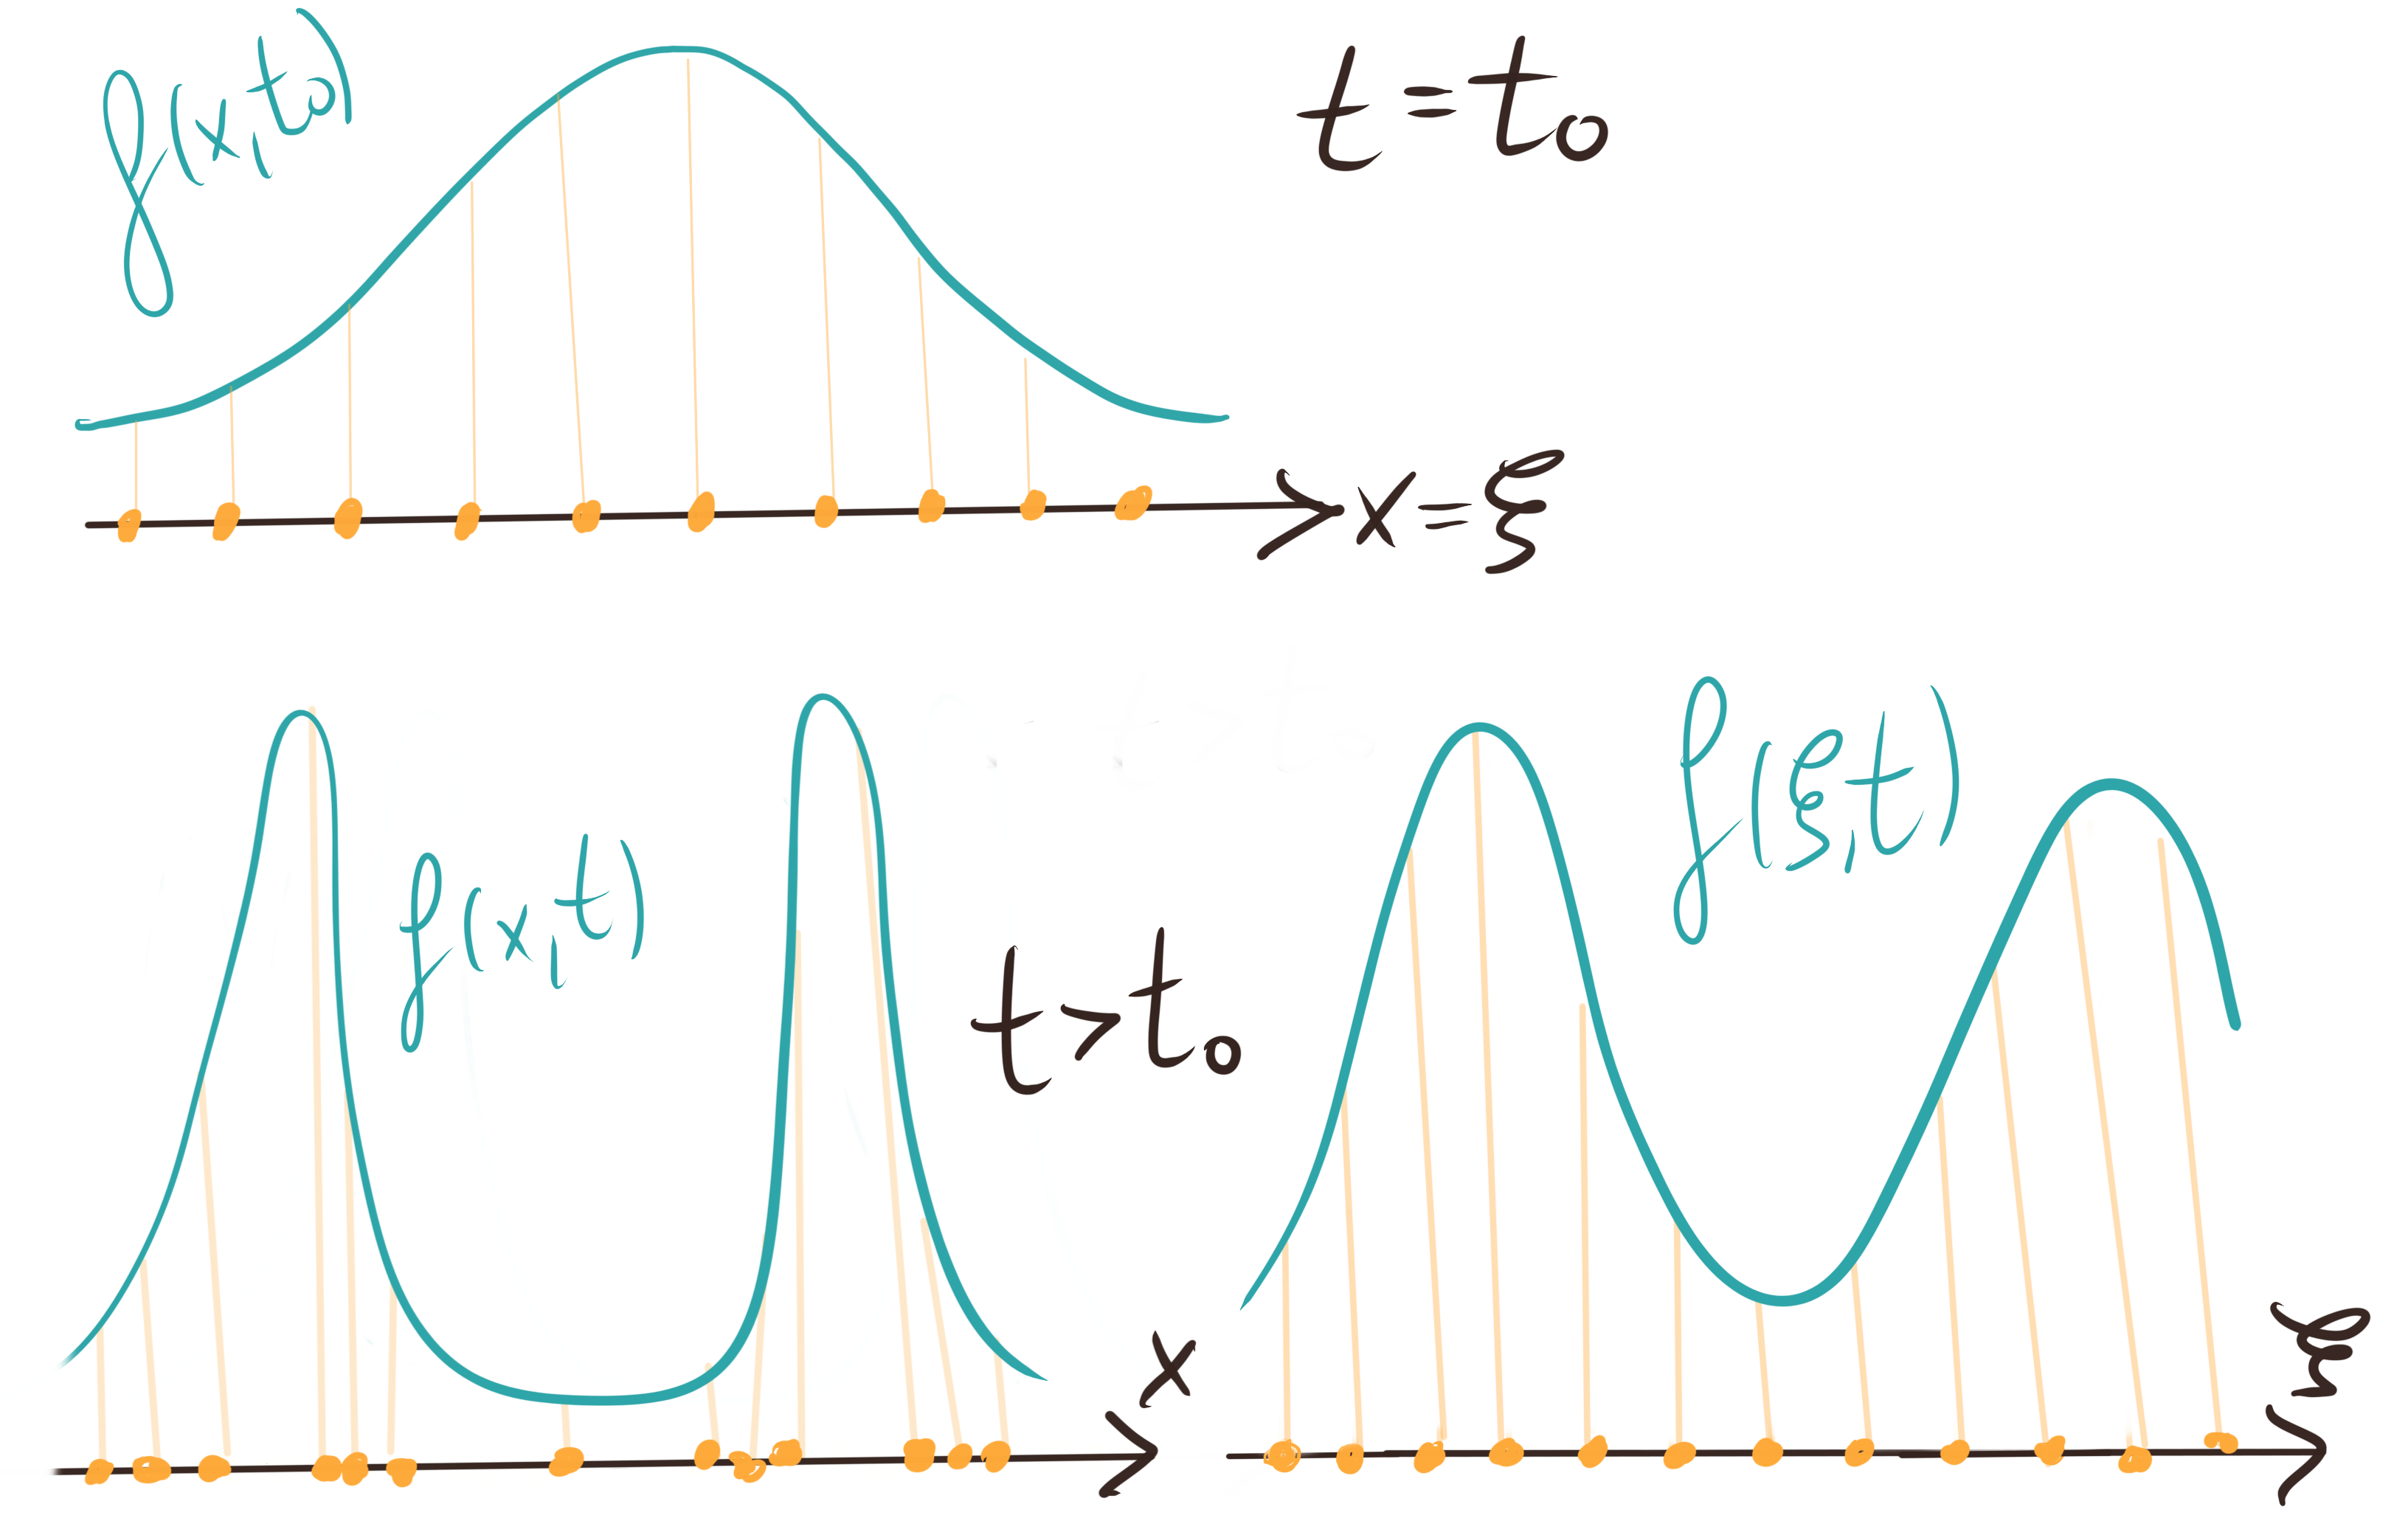
\includegraphics[width=0.50\linewidth]{8equidistribution.png}
  \caption{ Visual intuition of the equidistribution principle. Above the function at an initial reference time in which we define equispaced labels of the mesh elements (in yellow). Below left, we see the representation of where the same mesh elements should be in $x$ space in order to make the sum of the curvature of the function $f$ times their inter-distance be constant. The result (below right) is that the function at time $t$, as seen from the mesh element frame, is still well behaved, with no big variations. }
  \label{fig:equid}
\end{figure}
\newpage
Additionally, we could also adapt the grid to any other positive monitor of the system like $M(\vec{x},t)=\varepsilon+|\pdv{S(x,t)}{x}|$, $M(x,t)=\varepsilon+|\pdv[2]{S(x,t)}{x}|$, $M(x,t)=\varepsilon+c_1|\pdv{S(x,t)}{x}|+c_2|\pdv{\rho(x,t)}{x}|$ etc. Each would make the grid satisfy a different requirement.

Equation \eqref{discEq} are in reality $n-1$ equations with $n-2$ unknowns, since the boundaries of the grid $x^1, x^n$ are fixed by us (rather being still or following a certain trajectory, for instance a Bohmian one\footnote{This would allow the grid as a whole to follow the region of interest of the wave-function like in (II.g.2).}). This means, we can solve this in two ways: \vspace{-0.2cm}
\begin{itemize}
\item With an interpolation of the monitor by a sum of analytic functions, we can find the exact best grid. This would make the system of equations non-linear however, and would add the complication of the interpolation.

\item If we grossly approximate the values $M_j(t)$ as the value of the monitor function at say, the left corner of the interval, we could iteratively find the right corners of each grid cell, since the constant $C$ would be fixed.\vspace{-0.2cm}
\end{itemize}

Any of the two would define the positions of the grid elements such that they allow the equidistribution of the monitor function in each cell. The velocities are essential for the computation of the Lagrangian frame dynamical equations, so it is not enough with the values of the trajectory. We would then need to compute the grid element velocities necessary for this, using for instance $v^j(t)=\frac{x^j(t+\Delta t)-x^j(t)}{\Delta t}$, where $x^j(t)$ is the position of the mesh element at the last known time and $x^j(t+\Delta t)$ is the position of the mesh element in the following time.

This approach seems good so far, however, as we try to generalize it to an arbitrary $N$ we will notice that it is actually a rather too complicated numerical problem to solve.

A grid-cell for an arbitrary $N$ is the unit discretized volume element that partition the whole mesh volume. At the beginning, each of them will be an orthotope, but as we move around their vertices, the cells will loose their regular shape, just as we explained previously. In this case, this would make the discretization of the volume integral in each grid-cell non trivial, so an equation system like \eqref{discEq} would be hard to be explicitly found. To face this, we could restrict ourselves to the case in which we force the grid to be made of orthotopes. With this assumption, we could try to generalize the equidistribution idea, by first fixing the boundary grid points (leaving them just fixed or moving them according to some other criterium) and then looking for the inside grid points that allow the following integral to be constant:
\begin{equation}
\int_{x_1^j}^{x_1^{j+1}}\cdots \int_{x_N^k}^{x_N^{k+1}} M(\vec{x},t) dx_1 \cdots dx_N=C \quad \forall j\cdots \forall k
\end{equation}
If we discretize the integral we get:
\begin{equation}\label{monitor}
 M_{j,...,k}(t)\cdot (x_1^{j+1}-x_1^j)\ \cdots (x_N^{k+1}-x_N^k) =C \quad \forall j\cdots \forall k
\end{equation}
Where $M_{j,...,k}(t)$ is the local average of the monitor function evaluated at the vertices of the orthotope-cells. Forcing the cells to be orthotopes is equivalent to partitioning each axis in, say, $n$ points, meaning we will have $n^N$ mesh elements. We have about $(n-1)^N$ volume elements, so by fixing the boundaries of the region as we did in $N=1$, we can get the solution for the position of the new grid-elements as before: just by interpolating the monitor function with analytic functions and then solving the equation system, or by doing some gross approximation and solving in chain the equation system.

It is clear however, that this approach is not the one generating the most suitable grid, since we do not allow each mesh element to move in arbitrary directions.\footnote{ A good thing about this grid would be that it would be regular even if not equispaced.} There is however a very interesting alternative way to generalize the grid generation we described in $N=1$, that requires finding the continuum version of the discretized grid.

%In addition, we realize that now each mesh element can move in $N$ directions, meaning we will still have $(m-1)^N$ mesh-cells (if we initially discretize each axis in $m$ points) but there will be $m^N$ nodes each with $N$ numbers to fix. A total of $Nm^N$ unknowns. We should subtract the fixed positions of all the fixed boundary grid-points (which will in principle be chosen to be hyperplanes). However, we still see that there are more unknowns than equations. In addition, the equations are non-linear with no remedy and we must make an $N$ dimensional interpolation of the monitor function. 

\subsubsection*{(II.g.3.2) The continuum version of the dynamical mesh\vspace{-0.2cm}}
Note first that we are not really looking for independent nodes of a particular discrete grid, instead, we are looking for a diffeomorphism $\vec{x}(\vec{\xi},t)$, or an ensemble of continuous non-crossing trajectories that map the mesh at the initial time to a suitable mesh that allows us to have the field values evaluated at the points of interest. We will use vectors $\vec{\xi}\in\Omega_0\subset\R^N$ to tag the mesh elements, vectors reflecting their position in the initial grid. We will assume hereafter that this initial grid is chosen to be a regular Cartesian grid.

Now, note that, as we use unique $\vec{\xi}^j$ for the labelling of each mesh element, if we have that $||\vec{x}^{j+1}(t)-\vec{x}^j(t)||\rightarrow 0$, this must only be if $||\vec{\xi}^{j+1}-\vec{\xi}^j||\rightarrow 0$, since trajectories cannot cross and thus share a same position in configuration space at the same time. Then, this means that in equation \eqref{discEq}, the equalizer $C$ should get small in consonance with the distance between nodes. There must exist some $K\in\R$ such that $C=K(\xi^{j+1}-\xi^j)$, else the left hand side of \eqref{discEq} would go to zero while the right would not. If so, equation \eqref{discEq} becomes into:
\begin{equation}
M_j(t)\cdot \frac{x(\xi^{j+1},t)-x(\xi^{j},t)}{\xi^{j+1}-\xi^j}=K \quad \forall j
\end{equation}
Taking the limit of $\xi^{j+1}-\xi^j\rightarrow 0$, by definition this means that we are looking for:
\begin{equation}\label{contEq}
M(\xi,t)\cdot \pdv{x(\xi,t)}{\xi}=K \quad \forall \xi\in \Omega_0\subset \R
\end{equation}
If we recall that the signed Jacobian of the $N=1$ transformation is: $J(\xi,t)\equiv det(D_{\xi}x(\xi,t))=\pdv{x(\xi,t)}{\xi}$, then the above equation is equivalent to:
\begin{equation}
M(\xi,t)\cdot J(\xi,t)=K \quad \forall \xi\in \Omega_0\subset \R
\end{equation}
which is the continuum version of the equidistribution idea in equation \eqref{discEq}. Namely, the value of the monitor in each mesh element must be inversely proportional to the local divergence or convergence of trajectories, the local expansion or contraction of the grid. So we have found the continuum version of the equidistribution principle, which will be simpler to be generalized.

Alternatively, we can get rid of the constant $K$ in this last equation, if we make a further derivative:
\begin{equation}\label{EL1D}
\pdv{}{\xi}\qty(M(\xi,t)\cdot \pdv{x(\xi,t)}{\xi})=0 \quad \forall \xi\in \Omega_0\subset \R
\end{equation}
which can be manipulated to get:
\begin{equation}
\pdv[2]{x(\xi,t)}{\xi}+\pdv{}{\xi}log(M(\xi,t))\pdv{x(\xi,t)}{\xi}=0
\end{equation}
with boundary conditions $x(\xi^1,t)=a(t)$ and $x(\xi^n,t)=b(t)$. These conditions are the moving boundaries of the grid, that we are free to choose (even to follow Bohmian trajectories).

In particular, we can get the value of $K$ if we integrate equation \eqref{contEq} in $\xi$, in its domain $\Omega_0=\{\xi\in(\xi^1,\xi^n)\}$:
\begin{equation}
\int^{\xi^n}_{\xi^1} M(\xi,t) \pdv{x(\xi,t)}{\xi} d\xi=\int^{\xi^n}_{\xi^1} K d \xi  \Leftrightarrow \int^{x(\xi^n,t)}_{x(\xi^1,t)} M(x(\xi,t),t) dx(\xi,t)=K(\xi^n-\xi^1)
\end{equation}
\begin{equation}
K(t)=\frac{1}{(\xi_m-\xi_1)}\int^{b(t)}_{a(t)} M(x,t) dx
\end{equation}

Using that $M(\xi,t)>0$ $\forall \xi,t$, we could also integrate a little manipulation of equation \eqref{contEq} to get an expression for the grid we are looking for:
\begin{equation}
\int^{\xi^n}_{\xi^1}  \pdv{x(\xi,t)}{\xi} d\xi=\int^{\xi^n}_{\xi^1} \frac{1}{M(\xi,t)} K d \xi  \Leftrightarrow x(\xi,t)-x(\xi^1,t) =K(t)\int^{\xi^n}_{\xi^1} \frac{1}{M(\xi,t)}  d \xi
\end{equation}
\begin{equation}
x(\xi,t)=a(t)+K(t)\int^\xi_{\xi_1} \frac{1}{M(\xi,t)}d\xi
\end{equation}
This would allow us the straightforward computation of the dynamic grid. In fact, we get an alternative, perhaps computationally more tasty formula for $K(t)$ if we use $\xi=\xi_m$:
\begin{equation}
K(t)=(b(t)-a(t))\frac{1}{\int^{\xi_m}_{\xi_1} \frac{1}{M(\xi,t)}d\xi}\vspace{-0.2cm}
\end{equation}

\subsubsection*{\bf (II.g.3.3) Using a variational/optimization approach}
We will now show, closely following the brilliant exposition of Reference \cite{movingGrids}, that this could have equivalently been derived from an optimization problem (a variational one). Together with the preceding, this will be the way to explain how we can generalize the grid generation to arbitrary $N$, following the reference as well.

First let us express a discrete optimization problem, by defining a discrete functional the minimum of which will need to obey equation \eqref{discEq}. Suppose we are looking for a set of grid points $\{x^j \}_{j=1}^n$ such that the product of the interval lengths they leave and the average value of the monitor $M(x,t)$ in the interval, $M_j(t)$, is minimum. That is, we are looking for the $\R^n$ minimum of:  \vspace{-0.1cm}
\begin{equation}\label{discFunc}
S( x^1,...,x^n;t)=\sum_{j=1}^{m-1} \frac{1}{2} M_j(t) \qty(x^{j+1}-x^j)^2 \vspace{-0.1cm}
\end{equation}
with the conditions $x^1=a(t)$, $x^n=b(t)$. If we seek $S$ to be minimum, we also seek the products $M_j(t) \qty(x^{j+1}-x^j)^2$ to be minimum, which means that if the monitor $M$ gets big at a certain interval, the length of the interval $\qty(x^{j+1}-x^j)^2$ will get smaller. Just as we wanted.

If we are looking for the vector/grid $(x^1,...,x^n)$ that minimizes $S$ at a certain $t$, we will require that the gradient of $S$ at that point is zero. As such:
\begin{equation}
\pdv{S}{x^j}\Big\rvert_{optimum}=0\ \ \forall j\Longleftrightarrow M_{j-1}(t)(x^j-x^{j-1})-M_j(t)(x^{j+1}-x^j)=0\ \ \forall j
\end{equation}
This means that we must have the same product for all the adjacent intervals:
\begin{equation}
 M_{j-1}(t)(x^j-x^{j-1})=M_j(t)(x^{j+1}-x^j)\ \ \forall j
\end{equation}
Which is equivalent to ask that all the products are equal to a same number $C(t)$:
\begin{equation}
M_j(t)(x^{j+1}-x^j)=C(t) \quad \forall j
\end{equation}
which is exactly equation \eqref{discEq}. In fact, if one computes the Hessian matrix of the function $S$, one can see that the matrix is symmetric and positive semi-definite, meaning $S$ is convex, and has thus a single minimum at most. 

In fact, alternatively using as cost function (or discrete functional) the following one:\vspace{-0.1cm}
\begin{equation}
\hat{S}(x^1,...,x^n;t)=\sum_{j=1}^{m-1} \qty{\qty[ M_j(t) \qty(x^{j+1}-x^j)]^2-\qty[ M_j(t) \qty(x^{j}-x^{j-1})]^2}^2\vspace{-0.1cm}
\end{equation}
we get that the minimal is the same grid, meaning the discrete functional interpretation is not unique.

Now, let us obtain from here the continuous optimization problem that will lead us to the continuous version \eqref{contEq}. We will seek to minimize a cost function for possible functions $x(\xi,t)$: we will seek a functional $I[x(\xi,t)]$, the minimum of which will be required to satisfy the differential equation \eqref{contEq}. We could do this by inspection or by making the continuum limit of the previously described discrete functional. We will follow this last way.

If we divide both sides of equation \eqref{discFunc} by the increment $\Delta \xi$ of the labelling space grid we can have:
\begin{equation}
\frac{S( x^1,...,x^n;t)}{\Delta\xi}=\sum_{j=1}^{m-1} \frac{1}{2} M_j(t) \qty(\frac{x^{j+1}-x^j}{\Delta \xi})^2 \Delta \xi
\end{equation}
As we let $\Delta \xi \rightarrow 0$ and $n\rightarrow \infty$, we get by definition of integral:
\begin{equation}
I[x(\xi,t)]:=\lim\limits_{\substack{\Delta \xi \rightarrow 0\\ m \rightarrow \infty}}\frac{S( x^1,...,x^n;t)}{\Delta\xi}=\lim\limits_{\substack{\Delta \xi \rightarrow 0\\ m \rightarrow \infty}} \sum_{j=1}^{m-1}\frac{1}{2} M_j(t) \qty(\frac{x^{j+1}-x^j}{\Delta \xi})^2 \Delta \xi=\int_{\xi^1}^{\xi^n} M(\xi,t) \qty(\pdv{x(\xi,t)}{\xi})^2d\xi
\end{equation}
\begin{equation}\label{functional1D}
I[x(\xi,t)]=\int_{\xi^1}^{\xi^n} M(\xi,t) \qty(\pdv{x(\xi,t)}{\xi})^2d\xi
\end{equation}
$I$ is a functional, an operation outputting a number, a score, for each admissible $x(\xi,t)$ we input. In analogy with the discrete optimization problem, we will seek to find a diffeomorphism that minimizes the value of $I$. Note that this functional is nothing more than the Jacobian squared times the monitor function, summed over all the domain for $\xi$. Again, the same equidistribution interpretation holds. The minimization is subject to the requirement that the boundary of the mesh is fixed at $x(\xi_1,t)=a(t)$ and $x(\xi_m,t)=b(t)$.

The Euler-Lagrange equation for this functional (a necessary condition that $x(\xi,t)$ must obey) immediately gives us back equation \eqref{EL1D}, which is what we wanted.

\subsubsection*{\bf (II.g.3.4) The generalization of the dynamic grids to arbitrary N}

Knowing all this, in order to generalize it to an arbitrary $N$, we will follow the opposite approach than we tried in the beginning. We will first formulate continuum functionals and then get their related differential equations, which will rule the dynamics of the mesh. Additionally, we will explain another way to do so, by defining discrete functionals (cost functions for the grid nodes) and obtain linear equations to solve their minimization as a means of moving the grid.\vspace{-0.3cm}

\subsubsection*{\bf (\textalpha) A monitor per axis\vspace{-0.2cm}}
One possible way to generalize the functional in equation \eqref{functional1D} is noting that in $N=1$, $\pdv{x(\xi,t)}{\xi}$ is the covariant tangent vector of the $\xi$ axis. Its square $\qty(\pdv{x(\xi,t)}{\xi})^2$ could then be interpreted as the (positive) modulus of this covariant vector, which is the amount by which the grid spacing increases or decreases in that axis relative to the spacing of the label space. For each small increment of the label space coordinate $\xi$, how much the relative distance of those mesh elements has increased or decreased at time $t$. We could build a generalizing functional for arbitrary $N$ by defining first a set of monitor functions $M_1(\vec{\xi,t}),...,M_N(\vec{\xi},t)$ each of which we pretend to equalize with the grid spacing along each of the $N$ originally orthogonal axes $\xi_k$.
\begin{equation}
I[\vec{x}(\vec{\xi},t)]=\iint_{\Omega_0} \sum_{k=1}^N M_k(\vec{\xi},t) \Big|\Big|\pdv{\vec{x}(\vec{\xi},t)}{\xi_k}\Big|\Big|^2 d\xi
\end{equation}
In general, the system of $N$ Euler-Lagrange equations that minimizes this axis-wise product of the monitors times the mesh enlargement along each axis can be easily seen to be:
\begin{equation}
\pdv{}{\xi_1} \qty( M_1(\vec{\xi},t)\pdv{\vec{x}(\vec{\xi},t)}{\xi_1} )+\cdots+\pdv{}{\xi_N}\qty( M_N(\vec{\xi},t)\pdv{\vec{x}(\vec{\xi},t)}{\xi_N} )=0
\end{equation}
As we wanted, the $N=1$ case gets us back to equation \eqref{EL1D}.

In the $N=2$ case for example, we would have that we are minimizing:
\begin{equation}
I[\vec{x}(\xi_1, \xi_2,t)]=\iint_{\Omega_0} \Bigg\{M_1(\vec{\xi},t) \qty[\qty(\pdv{x_1(\xi_1,\xi_2,t)}{\xi_1})^2+\qty(\pdv{x_2(\xi_1,\xi_2,t)}{\xi_1})^2] +
\end{equation}
$$
M_2(\vec{\xi},t) \qty[\qty(\pdv{x_1(\xi_1,\xi_2,t)}{\xi_2})^2+\qty(\pdv{x_2(\xi_1,\xi_2,t)}{\xi_2})^2]\Bigg\} d\xi_1d\xi_2
$$
Its minimum, must be the transformation that satisfies the two differential equations:
\begin{equation}
\pdv{}{\xi_1} \qty( M_1(\vec{\xi},t)\pdv{x_k(\vec{\xi},t)}{\xi_1} )+\pdv{}{\xi_2}\qty( M_2(\vec{\xi},t)\pdv{x_k(\vec{\xi},t)}{\xi_2} )=0 \quad k\in\{1,2\}
\end{equation}
However, we can see that this is not exactly the equidistribution idea we had in the beginning, by which all the mesh elements are orchestrated in order to equalize a global monitor. Instead we are doing it differently for each axis.

\subsubsection*{\bf (\textbeta) The N-volume element functional}
In order to arrive to our original idea, we can realize that in equation \eqref{functional1D}, $(\pdv{x(\xi,t)}{\xi})^2$ is also the $N=1$ case of the squared determinant of the Jacobian matrix of the transformation, as we already anticipated. Remember that this gave us the separation increase factor between the trajectories $\vec{x}(\vec{\xi},t)$ of the mesh elements $\vec{\xi}$. How the grid contracts or expands locally in volume. Then, if we try to minimize the product of this Jacobian squared with a monitor function $M(\vec{\xi},t)$, we are trying to find the transformation $\vec{x}(\vec{\xi},t)$ that minimizes the functional:
\begin{equation}
I[\vec{x}(\vec{\xi},t)]=\iint_\Omega M(\vec{\xi},t) \qty(det(D_\xi \vec{x}(\vec{\xi},t)))^2 d\xi
\end{equation}
where note that we choose the square of the Jacobian, because we do not want the sign of the Jacobian to influence our choice for the transformation (the sign gives information about the local inversion of the coordinates), and this way the functional can have a minimum.

The system of $N$ Euler-Lagrange equations of this functional and thus the  system of differential equations that the transformation must follow is:
\begin{equation}
\sum_{k=1}^N \pdv{}{\xi_k} \qty( M(\vec{\xi},t) J \pdv{J }{\pdv{x_j}{\xi_k}} )=0\quad j\in\{1,...,N\}
\end{equation}
where we need to know the explicit shape of the Jacobian matrix determinant $J\qty(\pdv{x_i(\vec{\xi},t)}{\xi_j}):=det(D_\xi \vec{x}(\vec{\xi},t))$ to complete the expression. Note that the determinant only depends explicitly on terms $\pdv{x_i(\vec{\xi},t)}{\xi_j}$ with $i,j\in\{1,...,N\}$.

In $N=1$ this leads to equation \eqref{functional1D}, since $(det(D_\xi \vec{x}(\vec{\xi},t)))^2=\qty(\pdv{x(\xi,t)}{\xi})^2$, and consequently, the differential equation we would need to solve for getting the positions of the mesh elements would be equation \eqref{EL1D}.

In $N=2$, the functional we seek to minimize would be:
\begin{equation}
I[\vec{x}(\xi_1,\xi_2 ,t)]=\iint_\Omega M(\xi_1, \xi_2,t) \qty( \pdv{x_1}{\xi_1}\pdv{x_2}{\xi_2} - \pdv{x_1}{\xi_2} \pdv{x_2}{\xi_1})^2 d\xi
\end{equation}
the system of two Euler-Lagrange equations of which (the equation that the searched transformation must obey) is:
\begin{equation}
\pdv{}{\xi_1}\qty(M(\xi_1,\xi_2,t)J(\xi_1,\xi_2,t)\pdv{\vec{x}}{\xi_2})-\pdv{}{\xi_2}\qty(M(\xi_1,\xi_2,t)J(\xi_1,\xi_2,t)\pdv{\vec{x}}{\xi_1})=0
\end{equation}
with $J(\xi_1,\xi_2,t):=\pdv{x_1}{\xi_1}\pdv{x_2}{\xi_2} - \pdv{x_1}{\xi_2} \pdv{x_2}{\xi_1}$, the Jacobian.

\subsubsection*{\bf (\textgamma) Forcing the mesh to be orthogonal}
Even if we have already found the generalization we were looking for, note the relevance of this formalism in that we could actually invent custom functionals. For instance we could ask the mesh to preserve its orthogonality. A transformation $\vec{x}(\vec{\xi},t)$ will locally preserve the orthogonality if the covariant tangent vectors are mutually orthogonal: $\pdv{\vec{x}(\vec{\xi},t)}{\xi_k}\bullet \pdv{\vec{x}(\vec{\xi},t)}{\xi_j}=0\ \ \forall k\neq j$. We can try to impose this by looking for the transformation that minimizes the functional:
\begin{equation}
I[\vec{x}(\vec{\xi},t)]=\iint_\Omega \sum_{k\neq j} \qty(\pdv{\vec{x}(\vec{\xi},t)}{\xi_k}\bullet \pdv{\vec{x}(\vec{\xi},t)}{\xi_j})^2 d\xi
\end{equation}
Again, we consider the squared metric, in order to avoid negative projections between the covariant tangent vectors to make the functional hardly non-convex.
The system of $N$ Euler-Lagrange equations for this is:
\begin{equation}
\sum_{l=1}^N \pdv{}{\xi_l}\qty( \sum_{k=1;\ k\neq l}^N \qty[\pdv{\vec{x}(\vec{\xi},t)}{\xi_k}\bullet \pdv{\vec{x}(\vec{\xi},t)}{\xi_l}] \pdv{\vec{x}(\vec{\xi},t)}{\xi_j}  )=0
\end{equation}
The $N=2$ leaves:
\begin{equation}
\pdv{}{\xi_1}\qty( \qty[\pdv{\vec{x}(\vec{\xi},t)}{\xi_1}\bullet \pdv{\vec{x}(\vec{\xi},t)}{\xi_2}] \pdv{\vec{x}(\vec{\xi},t)}{\xi_2}  )+\pdv{}{\xi_2}\qty( \qty[\pdv{\vec{x}(\vec{\xi},t)}{\xi_1}\bullet \pdv{\vec{x}(\vec{\xi},t)}{\xi_2}] \pdv{\vec{x}(\vec{\xi},t)}{\xi_1}  )=0
\end{equation}
For the sake of numerical derivative computation, an orthogonal grid is always of good help. The problem is that there is no valid solution for many possible boundary conditions we could be interested on.

\subsubsection*{\bf (\textdelta) Using discretized functionals}

Just as we did in the $N=1$ case, instead of finding the time evolution of the mesh elements by solving the differential equations lead by the Euler-Lagrange equations of the continuous functionals, we could find the discretized versions of these functionals, or even invent some discrete functionals, and find their minimum by direct optimization, solving non-linear equation systems.

To do this, we formulate the problem in the following way: we seek the set of points $\{\vec{x}^j\in \Omega_t\}_{j=1}^{n^N}$ such that a cost function $S(\vec{x}^1,..,\vec{x}^{n^N})$ is minimized. Note we assume that we choose to have in the first iteration $n$ discrete points per axis, such that there are a total of $Nn^N$ unknowns. This cost function can be built by discretizing any continuous functional we have considered so far, or alternatively, by considering combinations of products of monitor functions with unit-cell angles, volumes, areas etc. 

Once we decide the cost function, we look for the grid $\{\vec{x}^j\in \Omega_t\}_{j=1}^{m^N}$ that makes its gradient be as close to zero as possible. This can be done by writing the equations explicitly, differentiating explicitly, and thus generating a system of $Nn^N$ coupled non-linear equations, or rather by using a gradient-descent like algorithm for local non-linear optimization.

The big advantage of this approach is that introducing the boundary conditions is typically simpler, since they are just conditions for the vectorial search space and can be trivially introduced. It is not as simple when we try to impose boundary conditions to a differential equation system.

\subsubsection*{\bf (\textepsilon) Mixing different functionals}
Both in the continuous or discrete functional cases, we can build new, perhaps more desirable, functionals, by choosing a weighted sum of the different functionals we have seen so far. For example, we could try to minimize the non-orthogonality at the same time that we try to force the equalization of a monitor function with the local $N$-volume increments.


\newpage

\fancyhead[L]{III . Part Lagrangian Part Eulerian Equations}


\section*{III . Part Lagrangian Part Eulerian Equations \vspace{-0.2cm}}
\addcontentsline{toc}{subsection}{\bf III . Part Lagrangian Part Eulerian Equations}
In this section, we will explore an intermediate approach between the Lagrangian and Eulerian frames. For this, we will consider that part of the system is observed in a Lagrangian frame, while the other part is considered in an Eulerian frame. The degrees of freedom described on the Eulerian frame will be denoted by $\vec{x}=(x_1,...,x_m)\in\R^m$ while the rest of degrees of freedom denoted by $\vec{y}=(x_{m+1},...,x_N)\in\R^{N-m}$ will be described as seen by Lagrangian frame fluid elements. If we need to refer to both kinds of variables at once, we will use $\vec{\x}=(\vec{x}, \vec{y})=(x_1,...,x_N)\in \R^N$.\vspace{-0.4cm}

\subsection*{If Only a subsystem is a Lagrangian fluid\vspace{-0.3cm}}

The most natural way (but not the one we will typically follow) to consider only a subsystem in the Lagrangian frame would be considering that only the degrees $\vec{y}$ represent a fluid. If so, we would label each fluid element using real vectors $\vec{\xi_y}\in\Gamma_0\subseteq \R^{N-m}$ representing their position $\vec{y}$ in the Lagrangian configuration-space at a reference time $t_0$, thus $\vec{\xi_x}:=\vec{y}( \vec{\xi_y},t_0)$. Since we would assume each fluid element follows the trajectory given by a {\em continuous} velocity field in configuration-space, by the Picard-Lindelöf theorem, there would exist a diffeomorphism $\vec{y}(\vec{\xi_y},t)\equiv \vec{y}^{\, \xi}(t) \quad \xi_y \in \Gamma_0 \subset \R^N$ giving their trajectories at all times. \vspace{-0.4cm}

\subsection*{Conditional Functions\vspace{-0.3cm}}

In order to have a geometric understanding of what having only part of the system in a Lagrangian frame means, before we dig deeper, consider a field $f(\vec{\x},t)$, where we evaluate its $\vec{y}$ coordinates at each time along the positions given by the trajectory $\vec{y}^{\, \xi}(t)$. We would then be considering the so called {\bf conditional function} $f(\vec{x}, \vec{y}^{\, \xi}(t),t)=f(\vec{x}, \vec{\xi}_y,t)\equiv f^\xi(\vec{x},t)$. Depending on the trajectory $\vec{\xi}_y$ we choose, the function $f(\vec{x}, \vec{y}^{\, \xi}(t),t)$ will represent a different moving   $m$ dimensional {\bf slice} of the $N$ dimensional field $f(\vec{\x},t)$. It is this why we will also call each possible set of degrees of freedom $\vec{y}$ a "transversal section" or "slice" of the system. You can see in Figure \ref{fig:slices} a visual representation of some conditional fields along different trajectories. Among others, we will deal with conditional wavefunctions $\psi(\vec{x}, \vec{y}^{\, \xi}(t),t)$ or conditional densities $\rho(\vec{x}, \vec{y}^{\, \xi}(t),t)$ and actions $S(\vec{x}, \vec{y}^{\, \xi}(t),t)$ as defined in the previous sections.\vspace{-0.3cm}


\begin{figure}[h!]
  \centering
    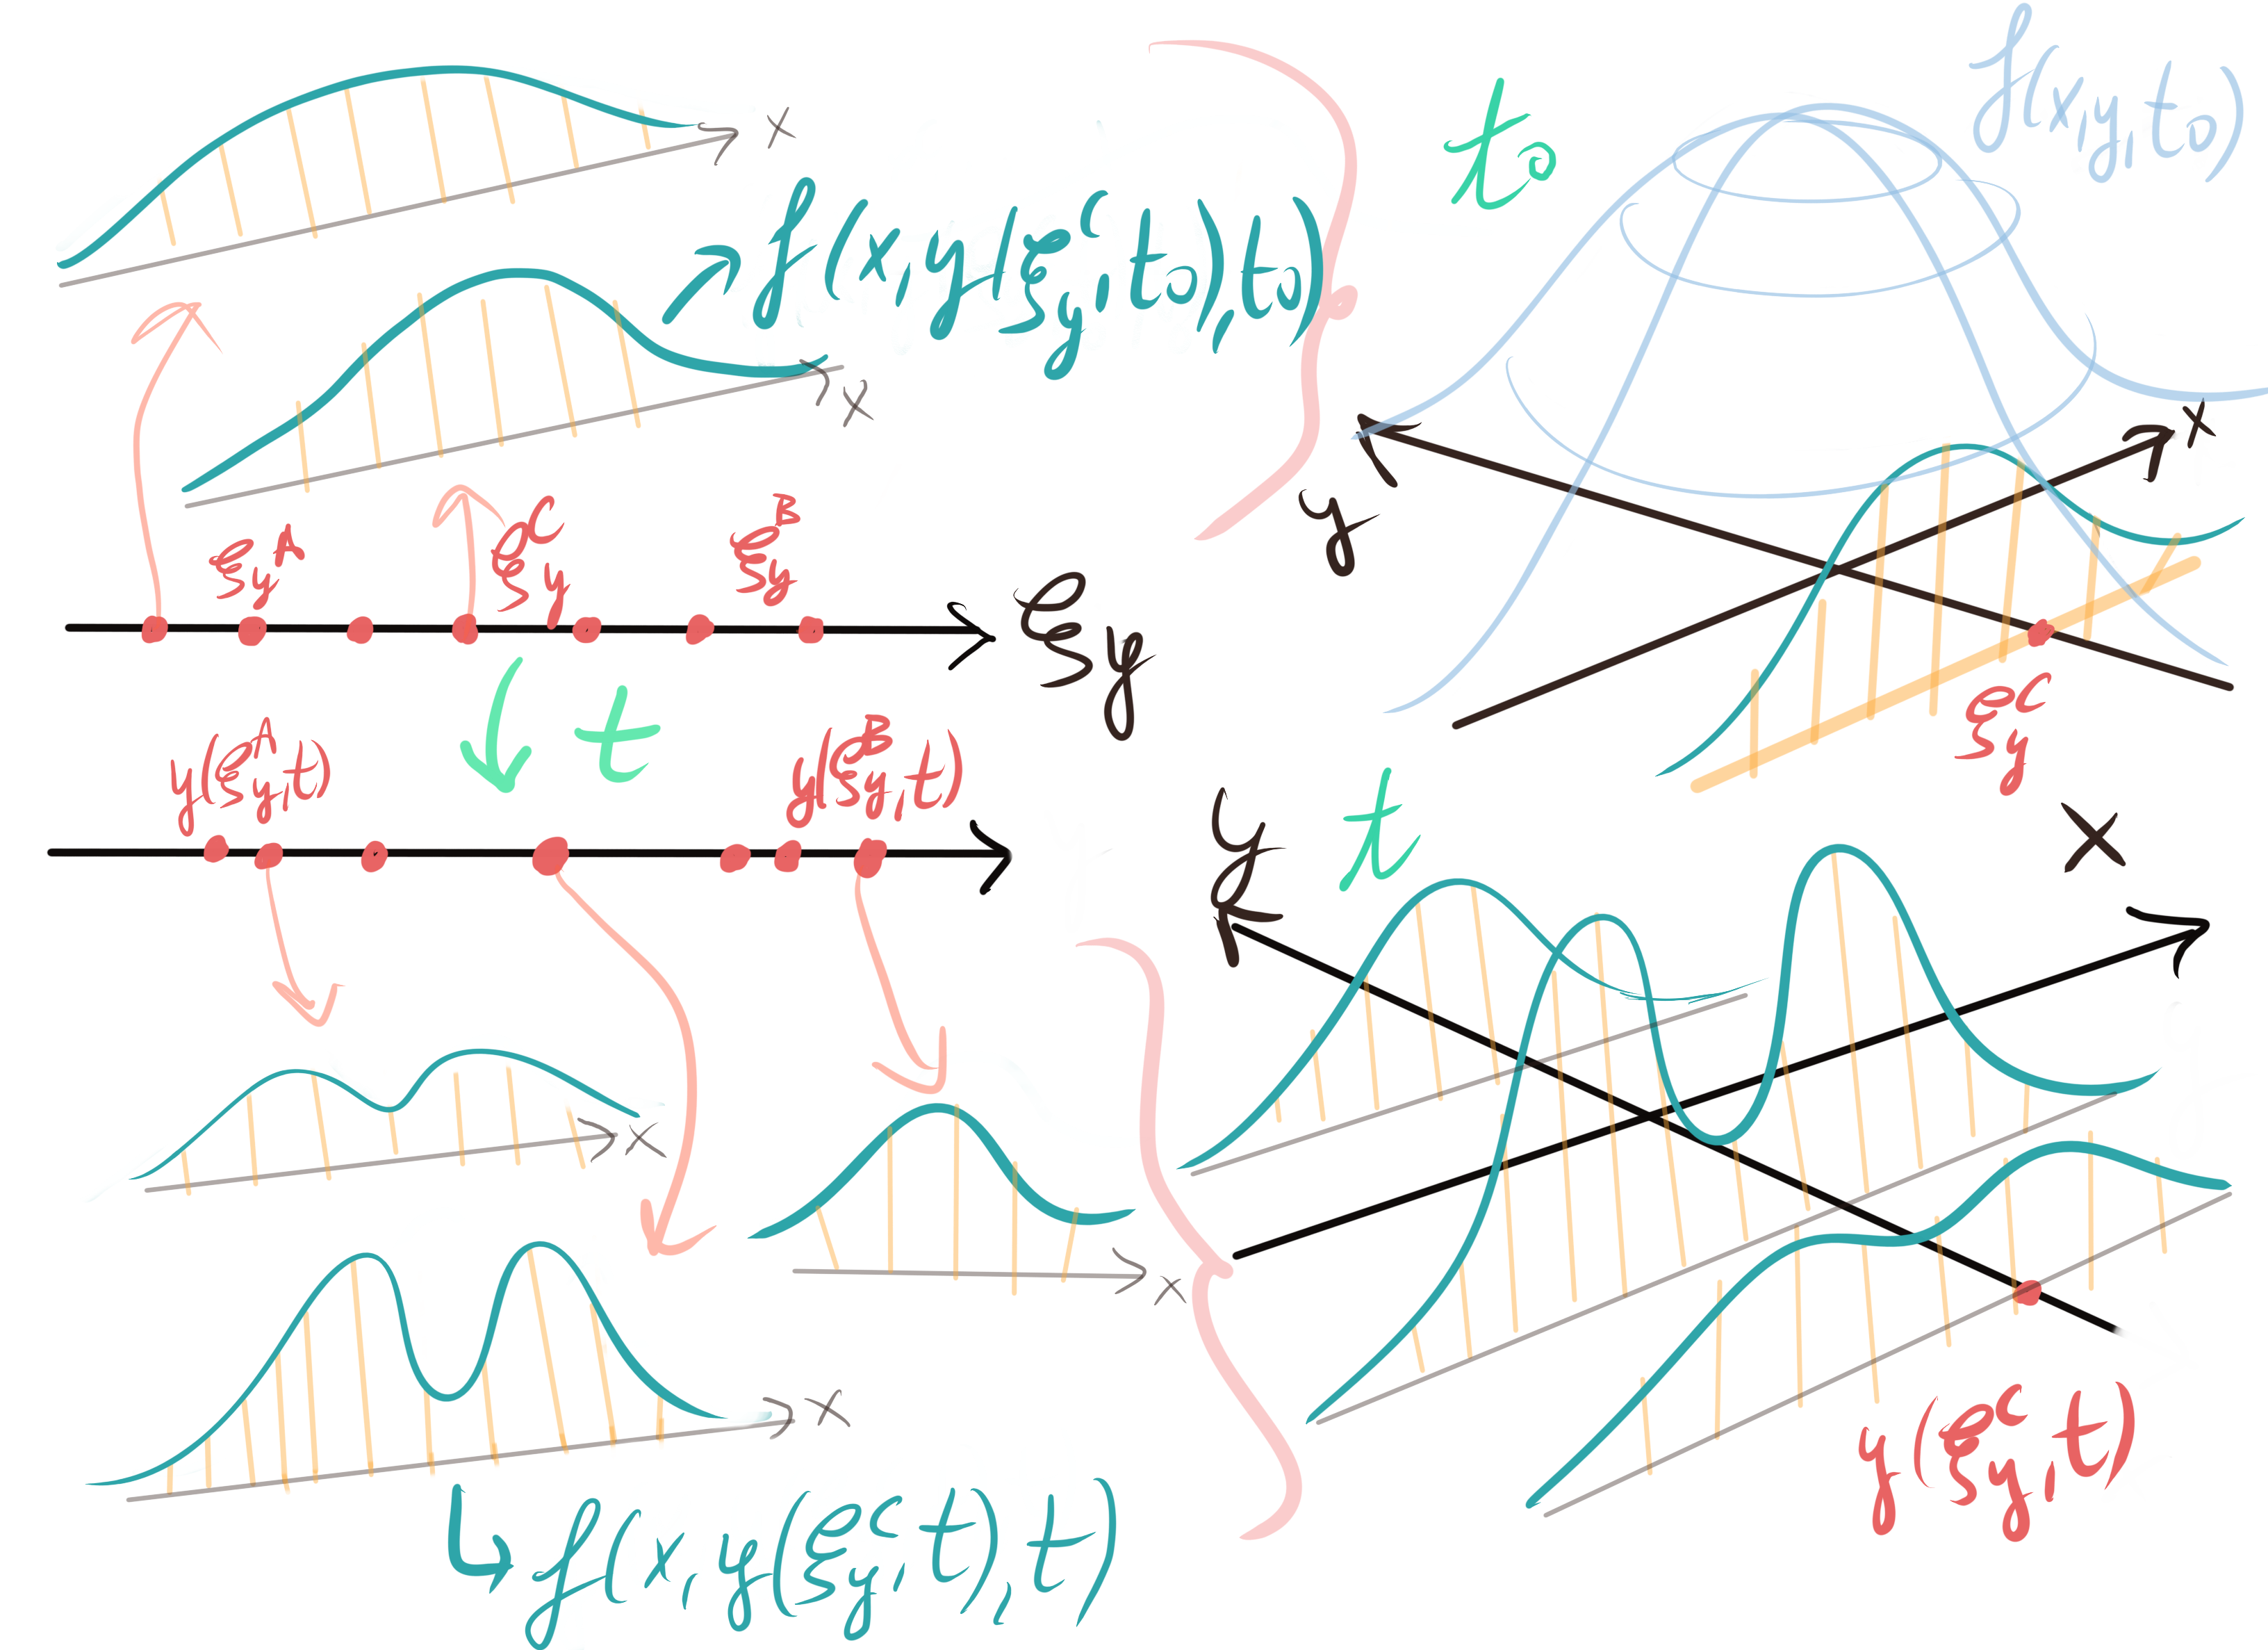
\includegraphics[width=0.70\linewidth]{6slices_1d.png}
  \caption{Conditional functions in $N=2$, where the $y$ axis is considered in the Lagrangian frame and $x$ in the Eulerian. In the center left, two axes represent the initial equidistant distribution of points $\xi_y$ in $y$ and their (non-equidistant) positions $y(\xi_y,t)$ after a time $t$. Each fluid element in $y$ has its own associated conditional function $f(x,y(\xi_y,t),t)$. If these are seen from the full function's $f(x,y,t)$ perspective, we can acknowledge they are slices, as depicted in the right (above the initial function and below the function at time $t$). These slices can give us an intuition of the full function.  }
  \label{fig:slices}
\end{figure}


\subsection*{Implicitly the full system is a Lagrangian fluid but explicitly only a subsystem\vspace{-0.2cm}}
In principle, considering only $\vec{y}$ as a moving continuum would be enough to describe the complete function $f(\vec{x},\vec{y},t)$ employing the conditional functions $f(\vec{x},\vec{y}(\vec{\xi}_y,t),t)$. Taking enough $\vec{\xi}_y$ we would have a slice of the full function at almost all the sections of interest. However, there are several reasons that will lead us to consider the degrees of freedom $\vec{x}$ as part of a fluid as well (as we did in the fully Lagrangian case), just that we will consider them as seen from an Eulerian frame.

{\bf Reason 1: Theoretical Homogeneity.} If we want to give physical meaning to the trajectories $\vec{y}(\vec{\xi}_y,t)$ alone, without viewing them as part of a trajectory of the full system, we will have a hard interpretative dilemma. If for example, $\vec{y}$ describes the degrees of freedom of the environment and $\vec{x}$ describes the degrees of our quantum experiment: for each possible point-like configuration of the environment, moving along its trajectory $\vec{y}(\vec{\xi}_y,t)$, we will have that our lab system is described by a continuous wavefunction $\psi(\vec{x},\vec{y}(\vec{\xi}_y,t),t)$. However, we should be able to symmetrically describe the environment using the Eulerian degrees $\vec{x}$ and our lab in the Lagrangian degrees $\vec{y}$, since we are working with physical laws that should not depend on the region of space we are looking at. If we did so, then our lab would be described by point-like configurations $\vec{y}(\vec{\xi}_y,t)$, while the environment would be a continuous wavefunction $\psi(\vec{x},\vec{y}(\vec{\xi}_y,t),t)$. It seems clear that rather we describe it all using a continuity of possibilities (a wavefunction) and/or all using a set of discrete configuration trajectories. This assertion is especially sustained by the fact that each time we conduct an experiment, we just find point like particles both in our lab and in the environment, but at the same time, we observe there is interference between the continuity of possible observed configurations in both the lab and the environment. Thus we should consider a whole trajectory of the lab and the environment together, and only then if we prefer it so, regard the lab in an Eulerian frame as a continuous wavefunction.

\begin{figure}[h!]
  \centering
    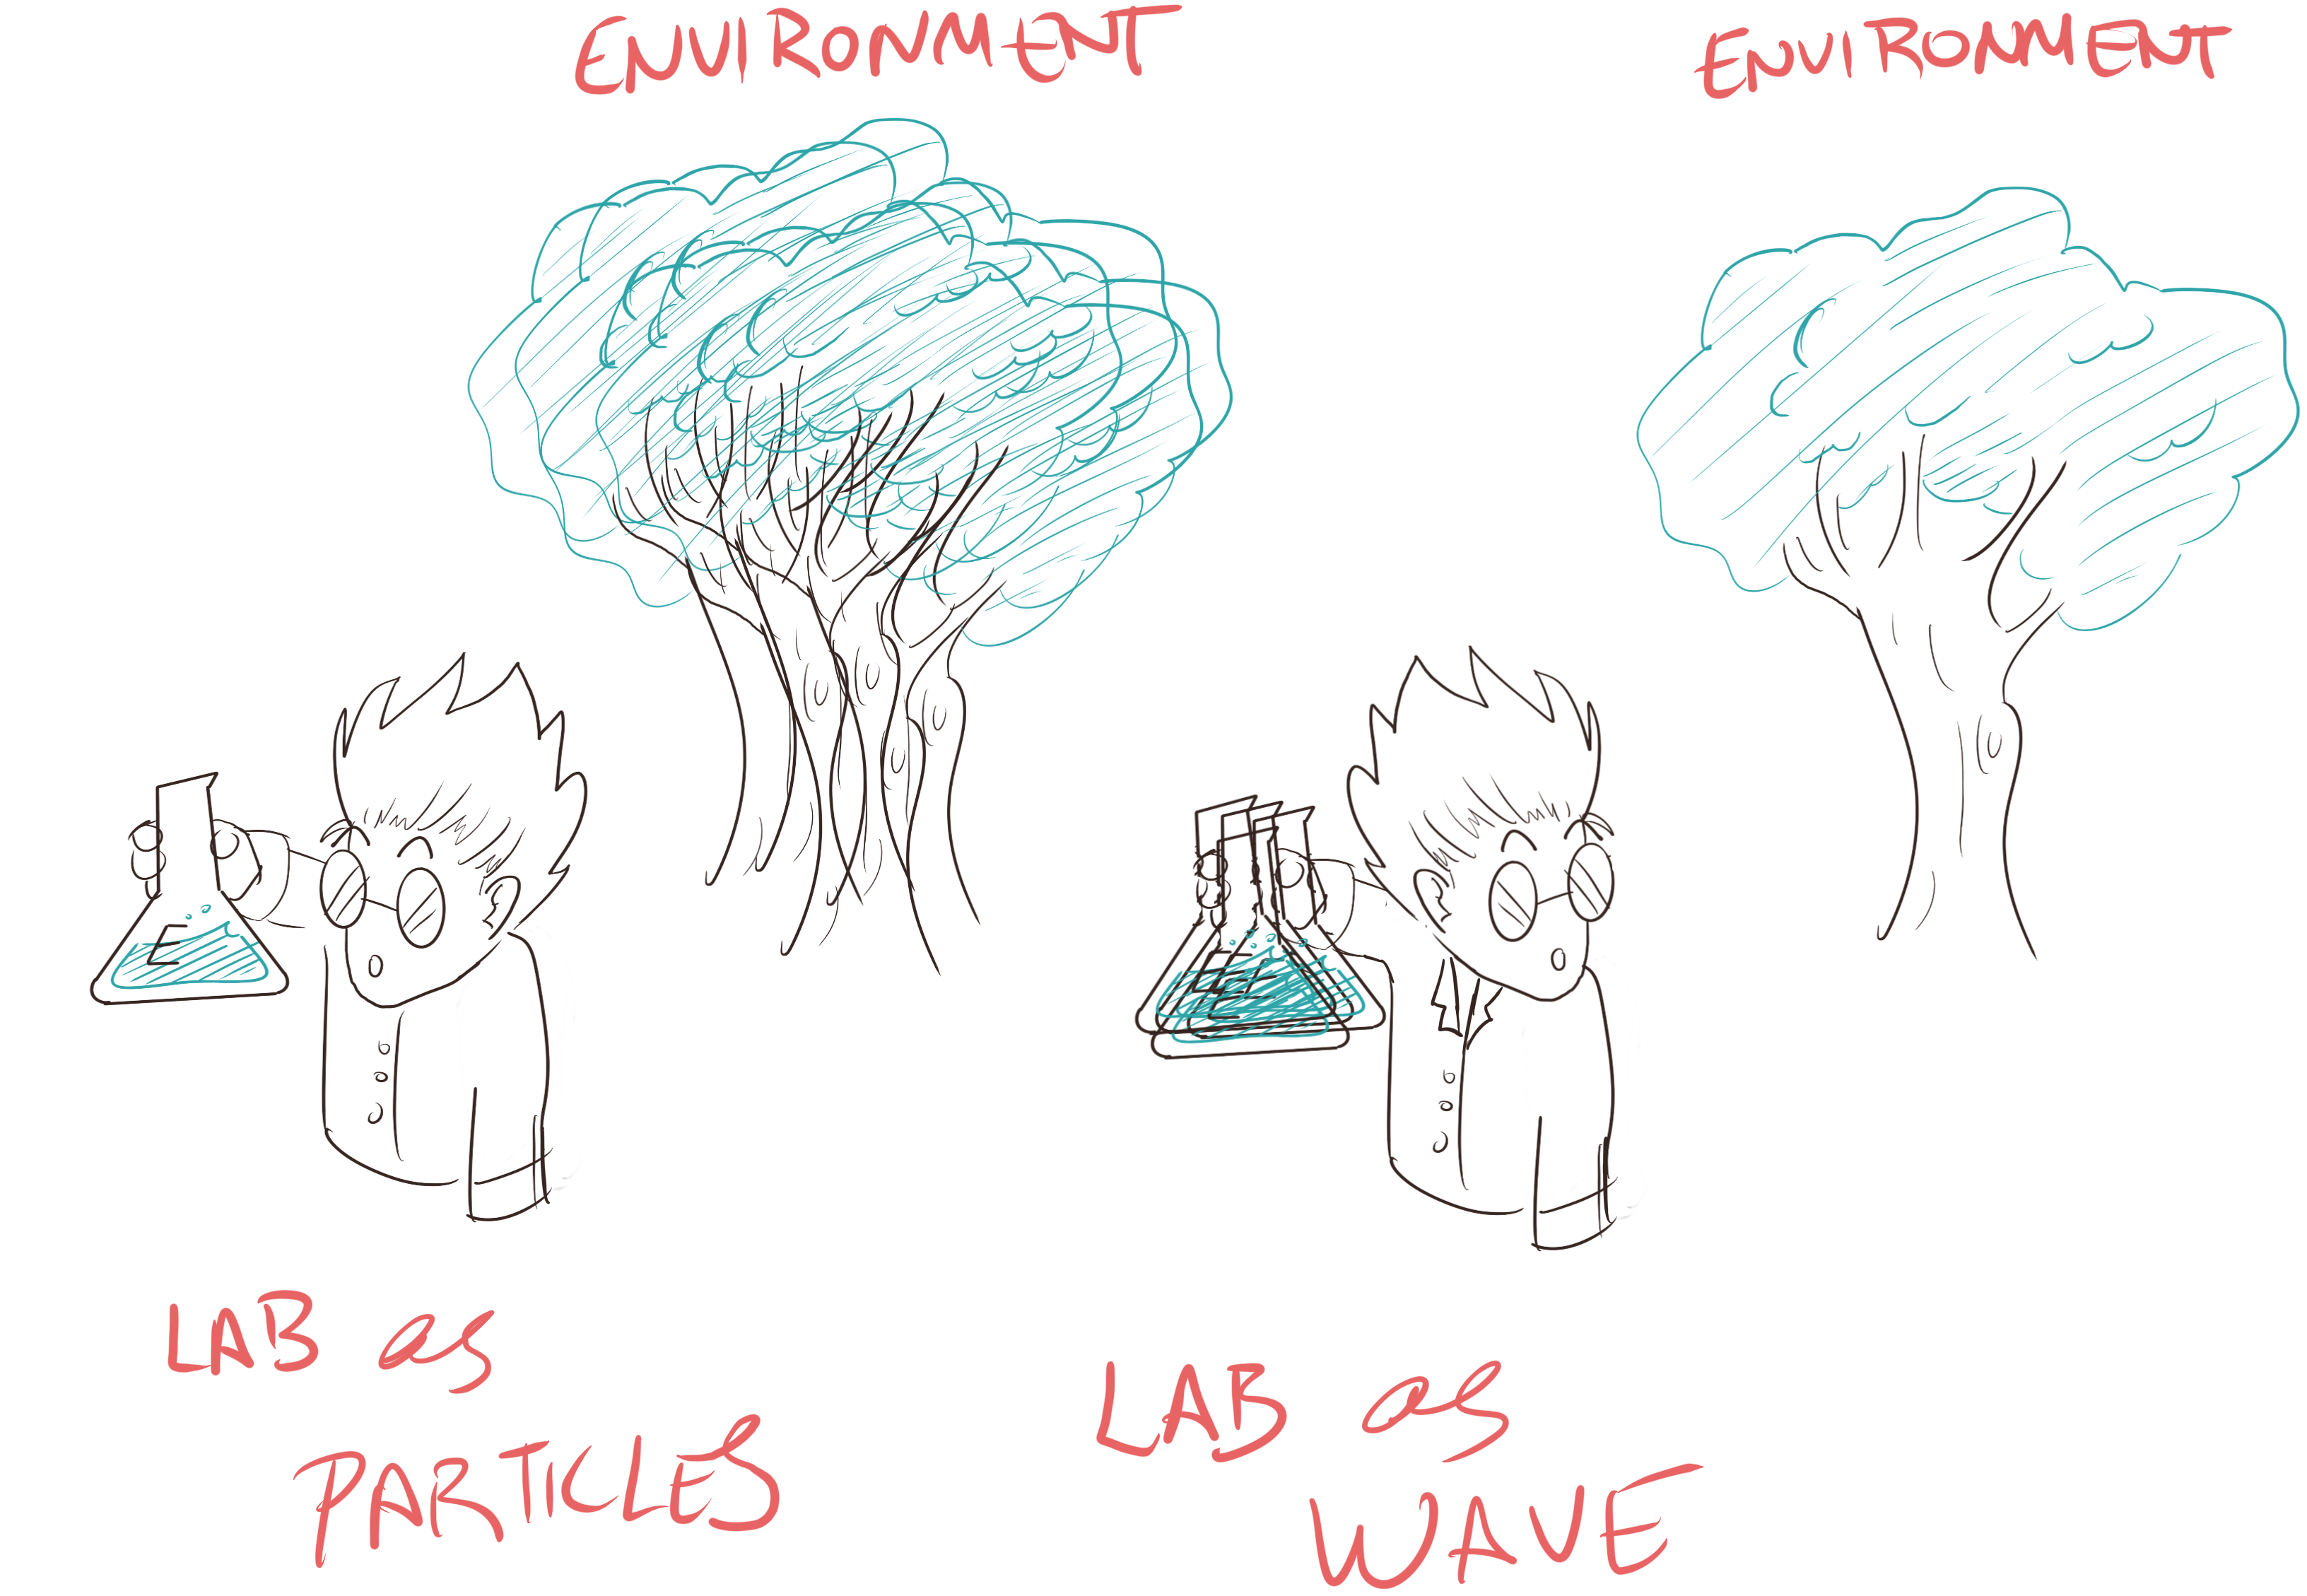
\includegraphics[width=0.64\linewidth]{labEnvironment.png}
  \caption{A cartoon showing the strange Universe in which we would live if depending on our choice of observation, part of the Universe would behave as a fluid of discrete particles and part as a continuous wavefunction. }
  \label{fig:jocoso}
\end{figure}

{\bf Reason 2: Reconciliation with Bohmian Trajectories.} If we try to describe the trajectory $\vec{y}(\vec{\xi}_y,t)$ using Bohmian trajectories, the trajectory will be badly defined, because for each possible $\vec{x}$, we will have a different velocity $\pdv{}{t}\vec{y}(\vec{\xi}_y,t)$ for the $\vec{\xi}_y$-th trajectory. This means that an initially univalued trajectory of the fluid element $\vec{\xi}_y$ will become multivalued. As a function of $\vec{x}$. We would be forced to describe it as $\vec{y}(\vec{\xi}_y, \vec{x},t)$. But what is the difference between this and considering directly that each position in $\vec{x}$ is as well part of a fluid element? None. As we will conclude from the following gray boxes, in order to describe Bohmian trajectories, we rather describe a trajectory for the full $N$ degree system, or we cannot have Bohmian trajectories. It makes no sense to talk about them for only a subsystem, without allusion to a trajectory of the whole.
\vspace{0.2cm}

\mybox{
\subsubsection*{What if we only considered Bohmian trajectory in $\vec{y}$?}

Let us see what would happen if we insisted on only considering the Lagrangian axes as a fluid and at the same time, we tried to attribute its fluid elements a Bohmian trajectory.\\

If we define the velocity field for $\vec{y}^{\, \xi}(t)=(x_{m+1}^\xi(t), ...,x_N^\xi(t))$ to be the Bohmian velocity field for those degrees of freedom:
\begin{equation}
\dv{}{t}x_j^\xi(t)=\frac{1}{m_j}\pdv{S(\vec{x}, \vec{y})}{x_j}\Big\rvert_{\vec{y}^{\, \xi}(t)}=\frac{\hbar^2}{m_j}\Im\qty( \psi^{-1} \pdv{\psi}{x_j})\Big\rvert_{\vec{y}^{\, \xi}(t)} \quad j\in\{m+1,...,N\}
\end{equation}
We will see that for each value of $\vec{x}=(x_1,...,x_m)$, the Eulerian degrees, we have a different velocity with which to move the trajectory in $\vec{y}$. This immediately tells us that the trajectory of the fluid element $\vec{\xi}_y$, that is $\vec{y}(\vec{\xi}_y,t)$, will get multivalued, at each $\vec{x}$ it will move to a different point in $\vec{y}$. This means we will need to parametrize the trajectory not only with its initial position $\vec{\xi}_y$ in $\vec{y}$, but also with a parameter representing the point $\vec{x}$ we are looking at to get the velocity. Thus using something like $\vec{y}(\vec{\xi}_y,t; \vec{x})$. Let us re-define this parameter as $\vec{\xi}_x\equiv \vec{x}$ (for obvious reasons). Since each $\vec{\xi}_x$ (or each $\vec{x}$), of this trajectory initially labelled by $\vec{\xi}_y$, only has a value of the conditional function over it, the conditional function $f(\vec{x},\vec{y}^{\, \xi}(\vec{\xi}_y,t; \vec{x}),t)$ is still a proper function in the Eulerian frame $f(\vec{x},\vec{y}^{\, \xi}(\vec{\xi}_y,t; \vec{x}),t)=f(\vec{x},t; \vec{\xi}_y)$. It is univalued for each Eulerian $\vec{x}$. However, if we view what is happening from the full function's perspective, we will have started with an affine slice of the full function, but in the moment we allow the trajectory position in $\vec{y}$ to have a different value per $\vec{x}$, what we know about the full function is a curved slice, as can be seen in Figure \ref{fig:only_y}.

}
\begin{figure}[h!]
  \centering
    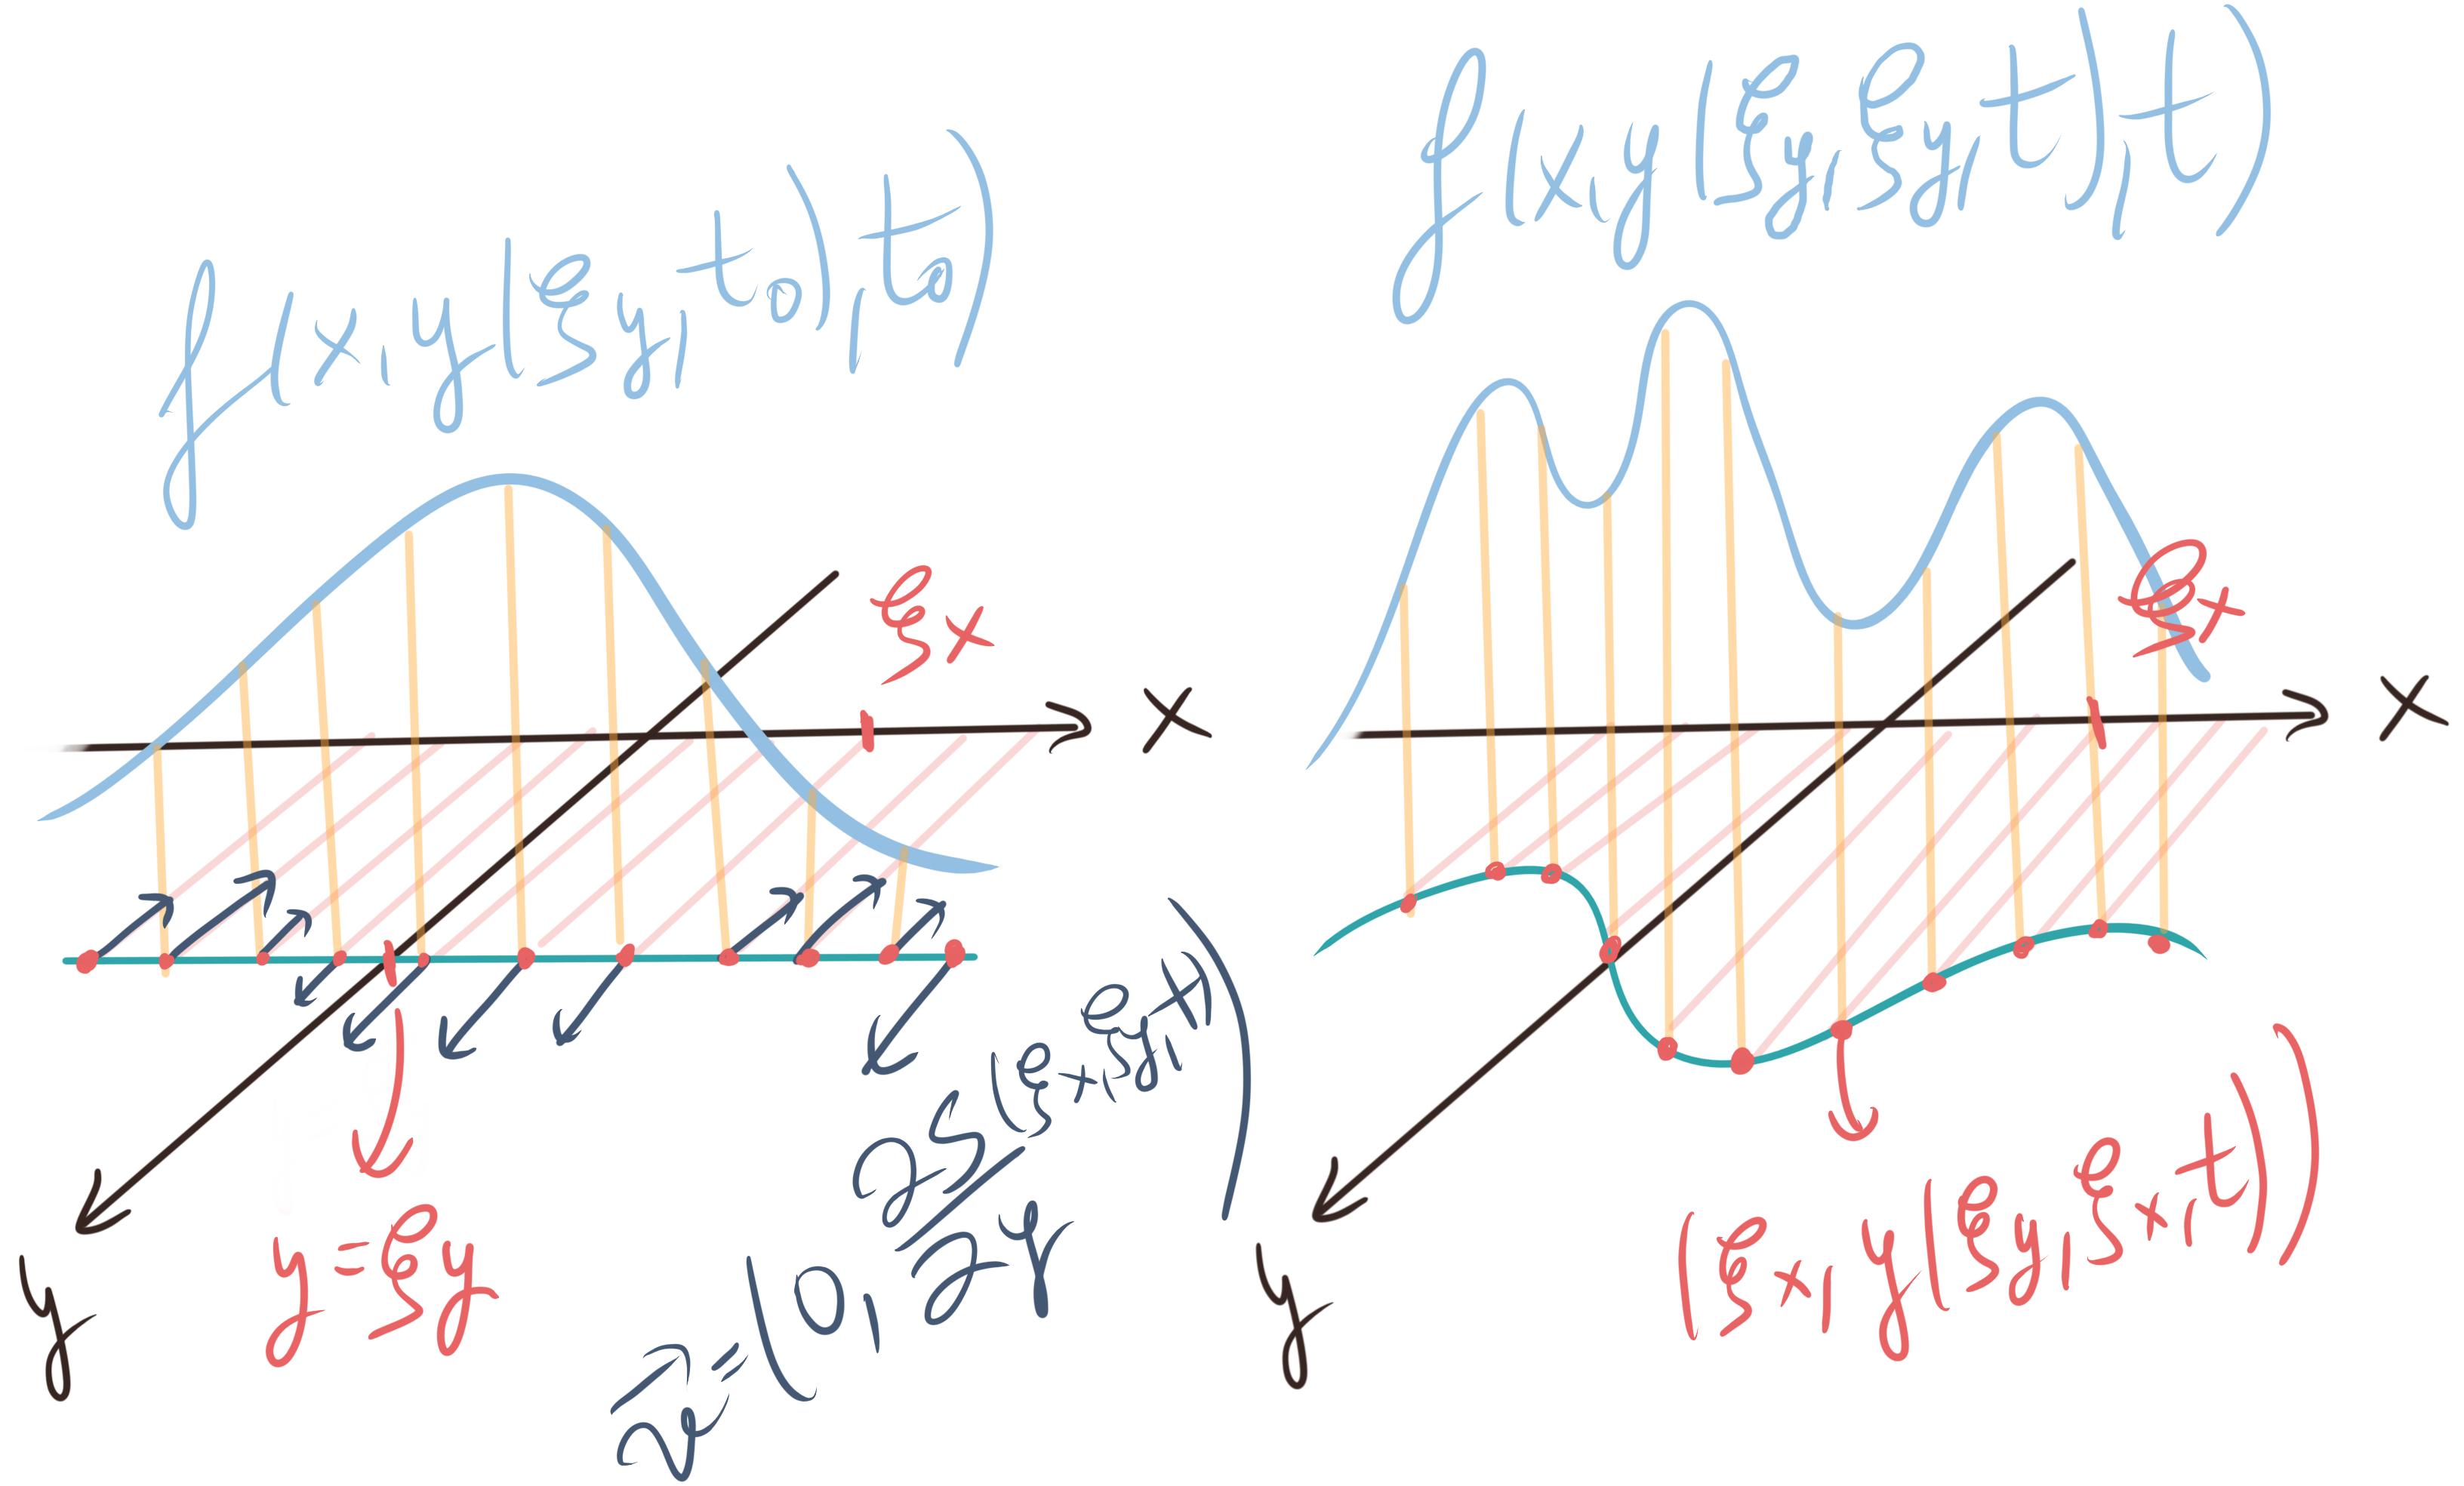
\includegraphics[width=0.65\linewidth]{unstructure_aligned.png}
  \caption{A conditional function for the fluid element $\vec{\xi}_y$. In the left, at time $t_0$, we see it has an $m$ dimensional affine support, but since each Eulerian degree is allowed to have its own version of the trajectory in $\vec{y}$, we get the curved slice in the right at time $t$. For each $\vec{x}$ there is still a single function value, but are the trajectories $\vec{y}(\vec{\xi}_y,t;\vec{x})$ Bohmian? %No as explained in the text.
  }
  \label{fig:only_y}
\end{figure}
\mybox{
In principle there is no problem, since the conditional function is still univalued per $\vec{x}$. But the concern comes when asking what are the trajectories we are obtaining: are we really knowing the Bohmian trajectories of the sub-system $\vec{y}$? The answer is no. If we view it from the full system Bohmian trajectory perspective, we are restricting the movement of the fluid elements to be still in $\vec{x}$, but the Bohmian velocity in $\vec{y}$ also depends on $\vec{x}$. The velocity for the degrees in $\vec{y}$ will be different if we allow moving in $\vec{x}$ or we restrict it. Thus, the obtained trajectories are not the subsystem part of the Bohmian trajectories.}%\footnote{
%Even if it will not be the approach we will use because it has a big problem to reconcile with Bohmian trajectories, as the equations for the conditional functions will be equivalent considering only $\vec{y}$ as a fluid or not, let us remark the main computational benefit of considering as a fluid only the subsystem $\vec{y}$. If we evolved several conditional functions for different initial positions in $y^\xi(t_0)=\xi^y_k$, the discretized $x$ points would always be aligned between the conditional functions, with the advantage that computing derivatives $\pdv{}{y}$ or interpolating in $y$ would be way simpler, even if the $y$ grid for each $x$ would get not equispaced with time. See Figure \ref{fig:only_y_grid}}
\mybox{
Instead, from the Fully Lagrangian perspective, what we are doing is define the trajectories:
\begin{equation}\label{a}
\begin{cases}
\vec{x}(\vec{\xi}_y, \vec{\xi}_x,t)=\vec{\xi}_x \quad \forall t\geq t_0\\
\vec{y}(\vec{\xi}_y, \vec{\xi}_x,t)=\vec{\xi}_y+\int_{t_0}^t \vec{v}_y(\vec{x}=\vec{\xi}_x, \vec{y}=\vec{y}(\vec{\xi}_y, \vec{\xi}_x,t),t)dt\\ \\
v_j(\vec{x}, \vec{y},t)=\frac{1}{m_j}\pdv{S(\vec{x}, \vec{y},t)}{x_j}\quad j\in\{m+1,...,N \}
\end{cases}
\end{equation}

%\begin{figure}[h!]
 % \centering
 %   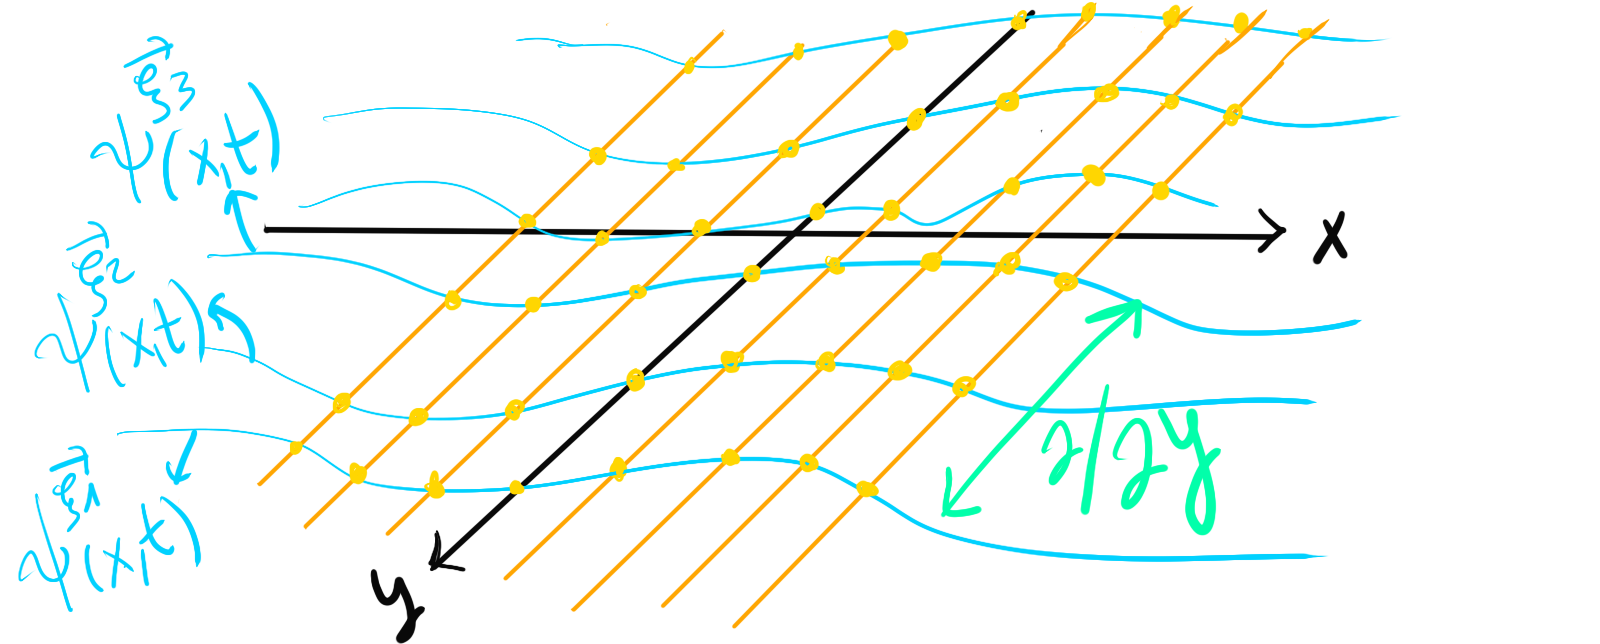
\includegraphics[width=0.65\linewidth]{aligned.png}
 % \caption{Blue lines represent the suppoort of CWF-s with different initial time $\xi^y_j$ after they evolve in time following  \eqref{a}. Note how the discretized points of all the CWF-s, the yellow dots, are aligned even at $t>t_0$, meaning operations like $\pdv{}{y}$ on each yellow element can be trivially done numerically. }
  %\label{fig:only_y_grid}
%\end{figure}

\subsection*{Falling back to the Fully Lagrangian Picture}
Thus, to really get Bohmian trajectories, we should not only allow the trajectory $\vec{\xi}_y$ in $\vec{y}$ to branch in a different value per $\vec{x}$, but we should also keep track of their movement in $\vec{x}$. Doing so, we would have that the points over which we consider the conditional function would be:
\begin{equation}
\begin{cases}\label{b}
\vec{x}^{\, \xi}(t)=\vec{\xi}_x +\int_{t_0}^t \vec{v}_x(\vec{x}(t), \vec{y}(t),t)dt\quad \forall t\geq t_0\\
\vec{y}^{\, \xi}(t)=\vec{\xi}_y+\int_{t_0}^t \vec{v}_y(\vec{x}(t), \vec{y}(t),t)dt\\ \\
v_j(\vec{x}, \vec{y},t)=\frac{1}{m_j}\pdv{S(\vec{x}, \vec{y},t)}{x_j}\quad j\in\{1,...,N \}
\end{cases}
\end{equation}


If we did so, as it can be seen in Figure \ref{fig:fallback}, each element of the initially affine Eulerian support of the conditional function would move in different directions in the $N$ axes of configuration-space. We would end up having a varying number of values of the same function $f$ for a same $\vec{x}$, which is incompatible with a proper univalued Eulerian function description. The support would still be an $m$ dimensional manifold, meaning the parametrization given by the initial position would be one to one for a certain $\vec{\xi}_y$. There would be only one point in the wavefunction per each $\vec{\xi}_x$ in the initial manifold. Thus, for a correct univalued description, we would require now to parametrize as well the conditional function support as a function of the initial position in $\vec{x}$, say using a parameter $\vec{\xi}_x$. However, this is exactly the definition of the Fully Lagrangian Picture, where there is a value of the function per point in the initial support manifold $f(\vec{x}(\vec{\xi},t), \vec{y}(\vec{\xi},t),t)=f(\vec{\xi},t)$.
}


\begin{figure}[h!]
  \centering
    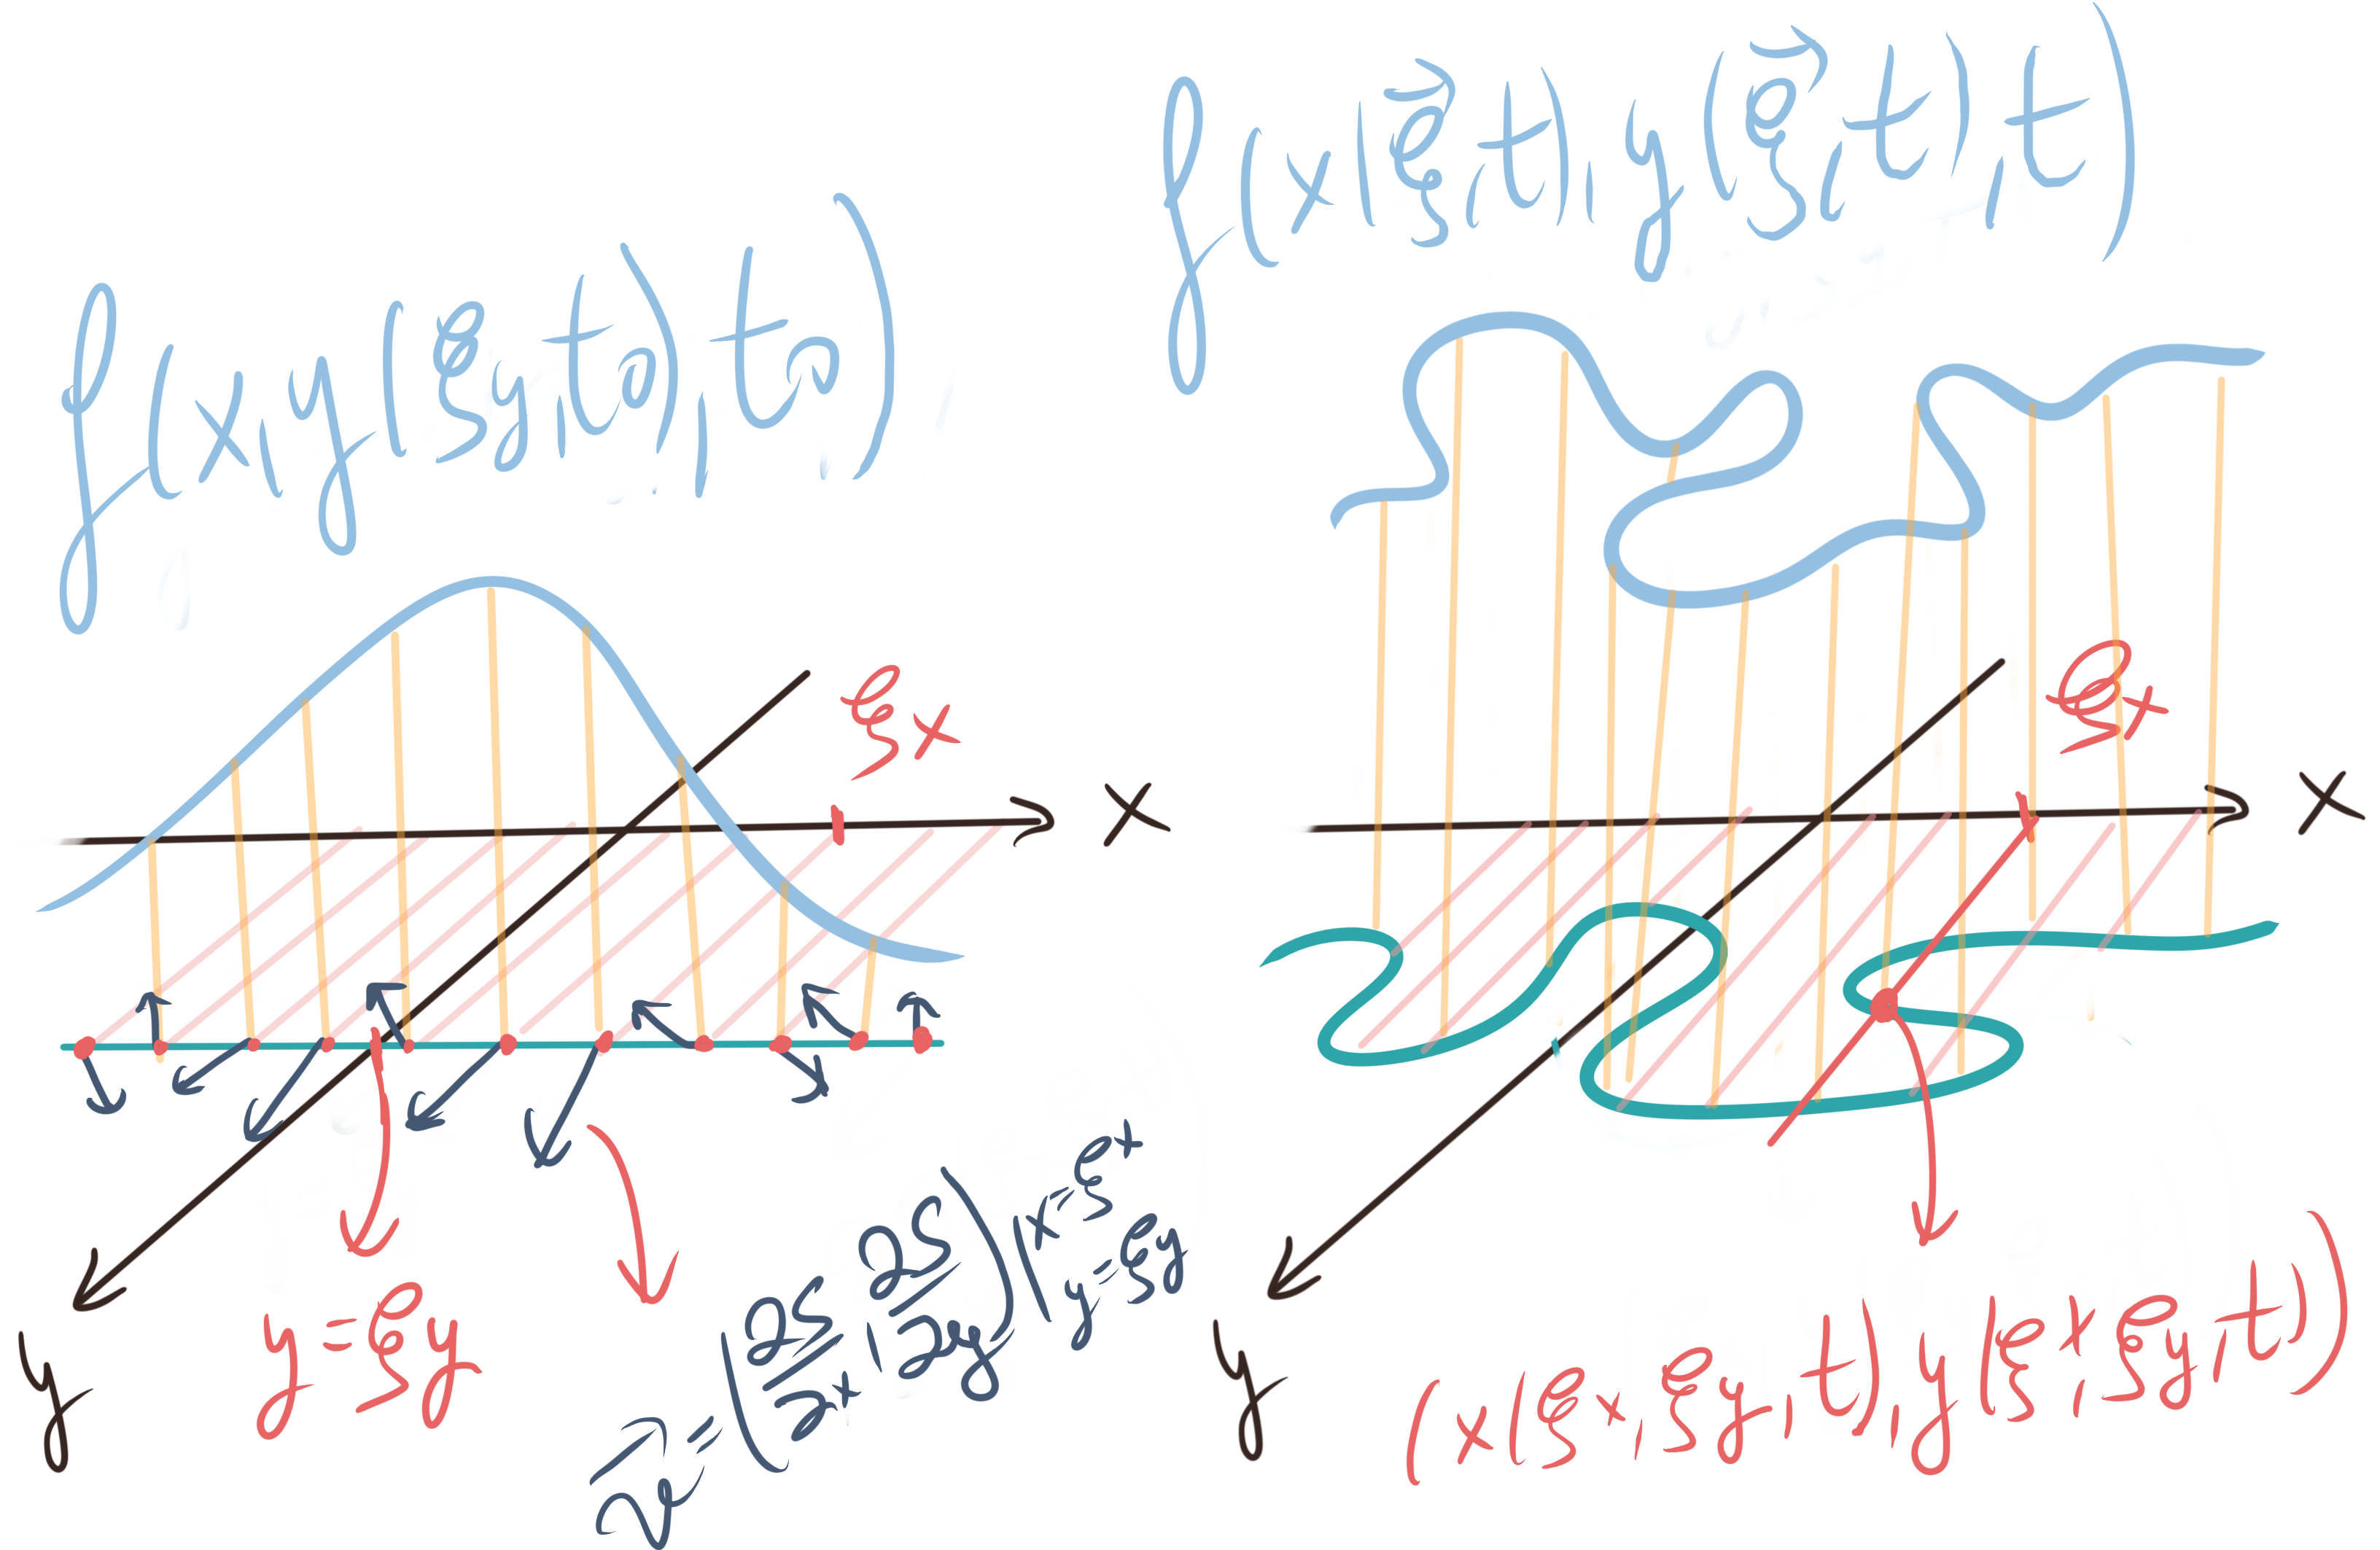
\includegraphics[width=0.65\linewidth]{unstructuring.png}
  \caption{A conditional function for the initial trajectory position $\vec{y}=\vec{\xi}_y$ in the left, with an affine support, but where each considered point will be evolved with a different velocity in $\R^N$. The result in a time $t>t_0$ can be seen in the right, where the support over which we are looking at the full function is a curve that can pass from the same value in $\vec{x}$ multiple times. To describe this conditional function, we will then require to parametrize the positions in $\vec{x}$ as well. We essentially fall back to the fully Lagrangian view of the function. }
  \label{fig:fallback}
\end{figure}

\mybox{
\subsection*{Solution: Evolve a single $\R^N$ Bohmian trajectory per conditional function}
We have found that even if we are only interested in Bohmian trajectories for the subsystem in $\vec{y}$, Bohmian trajectories require the implicit parametrization of the initial support of the conditional function both in $\vec{x}$ and $\vec{y}$ for a proper time evolution. That is, we need to describe implicitly the whole system as a fluid even if we will then see some degrees in the Eulerian frame. However, having each point of the support of the conditional function move according to Bohmian trajectories resulted in the fully Lagrangian frame. A solution to this impasse is to avoid all the points of the support to move independently. What if we forced all the points of the support of the conditional function to move along a {\bf single} Bohmian trajectory? We would then achieve our original idea. The wavefunction would remain univalued per each $\vec{x}$ at all times, meaning we could describe it in Eulerian terms, but at the same time we would get a Bohmian trajectory. See Figure \ref{fig:singleTraj}. 

Note very importantly that this leaves us a free choice to select   for the single trajectory we will evolve, which will be the initial $\vec{\xi}_x$ position among the Eulerian degree support. We could choose it randomly using the Born rule restricted to the section for example.

}
\begin{figure}[h!]
  \centering
    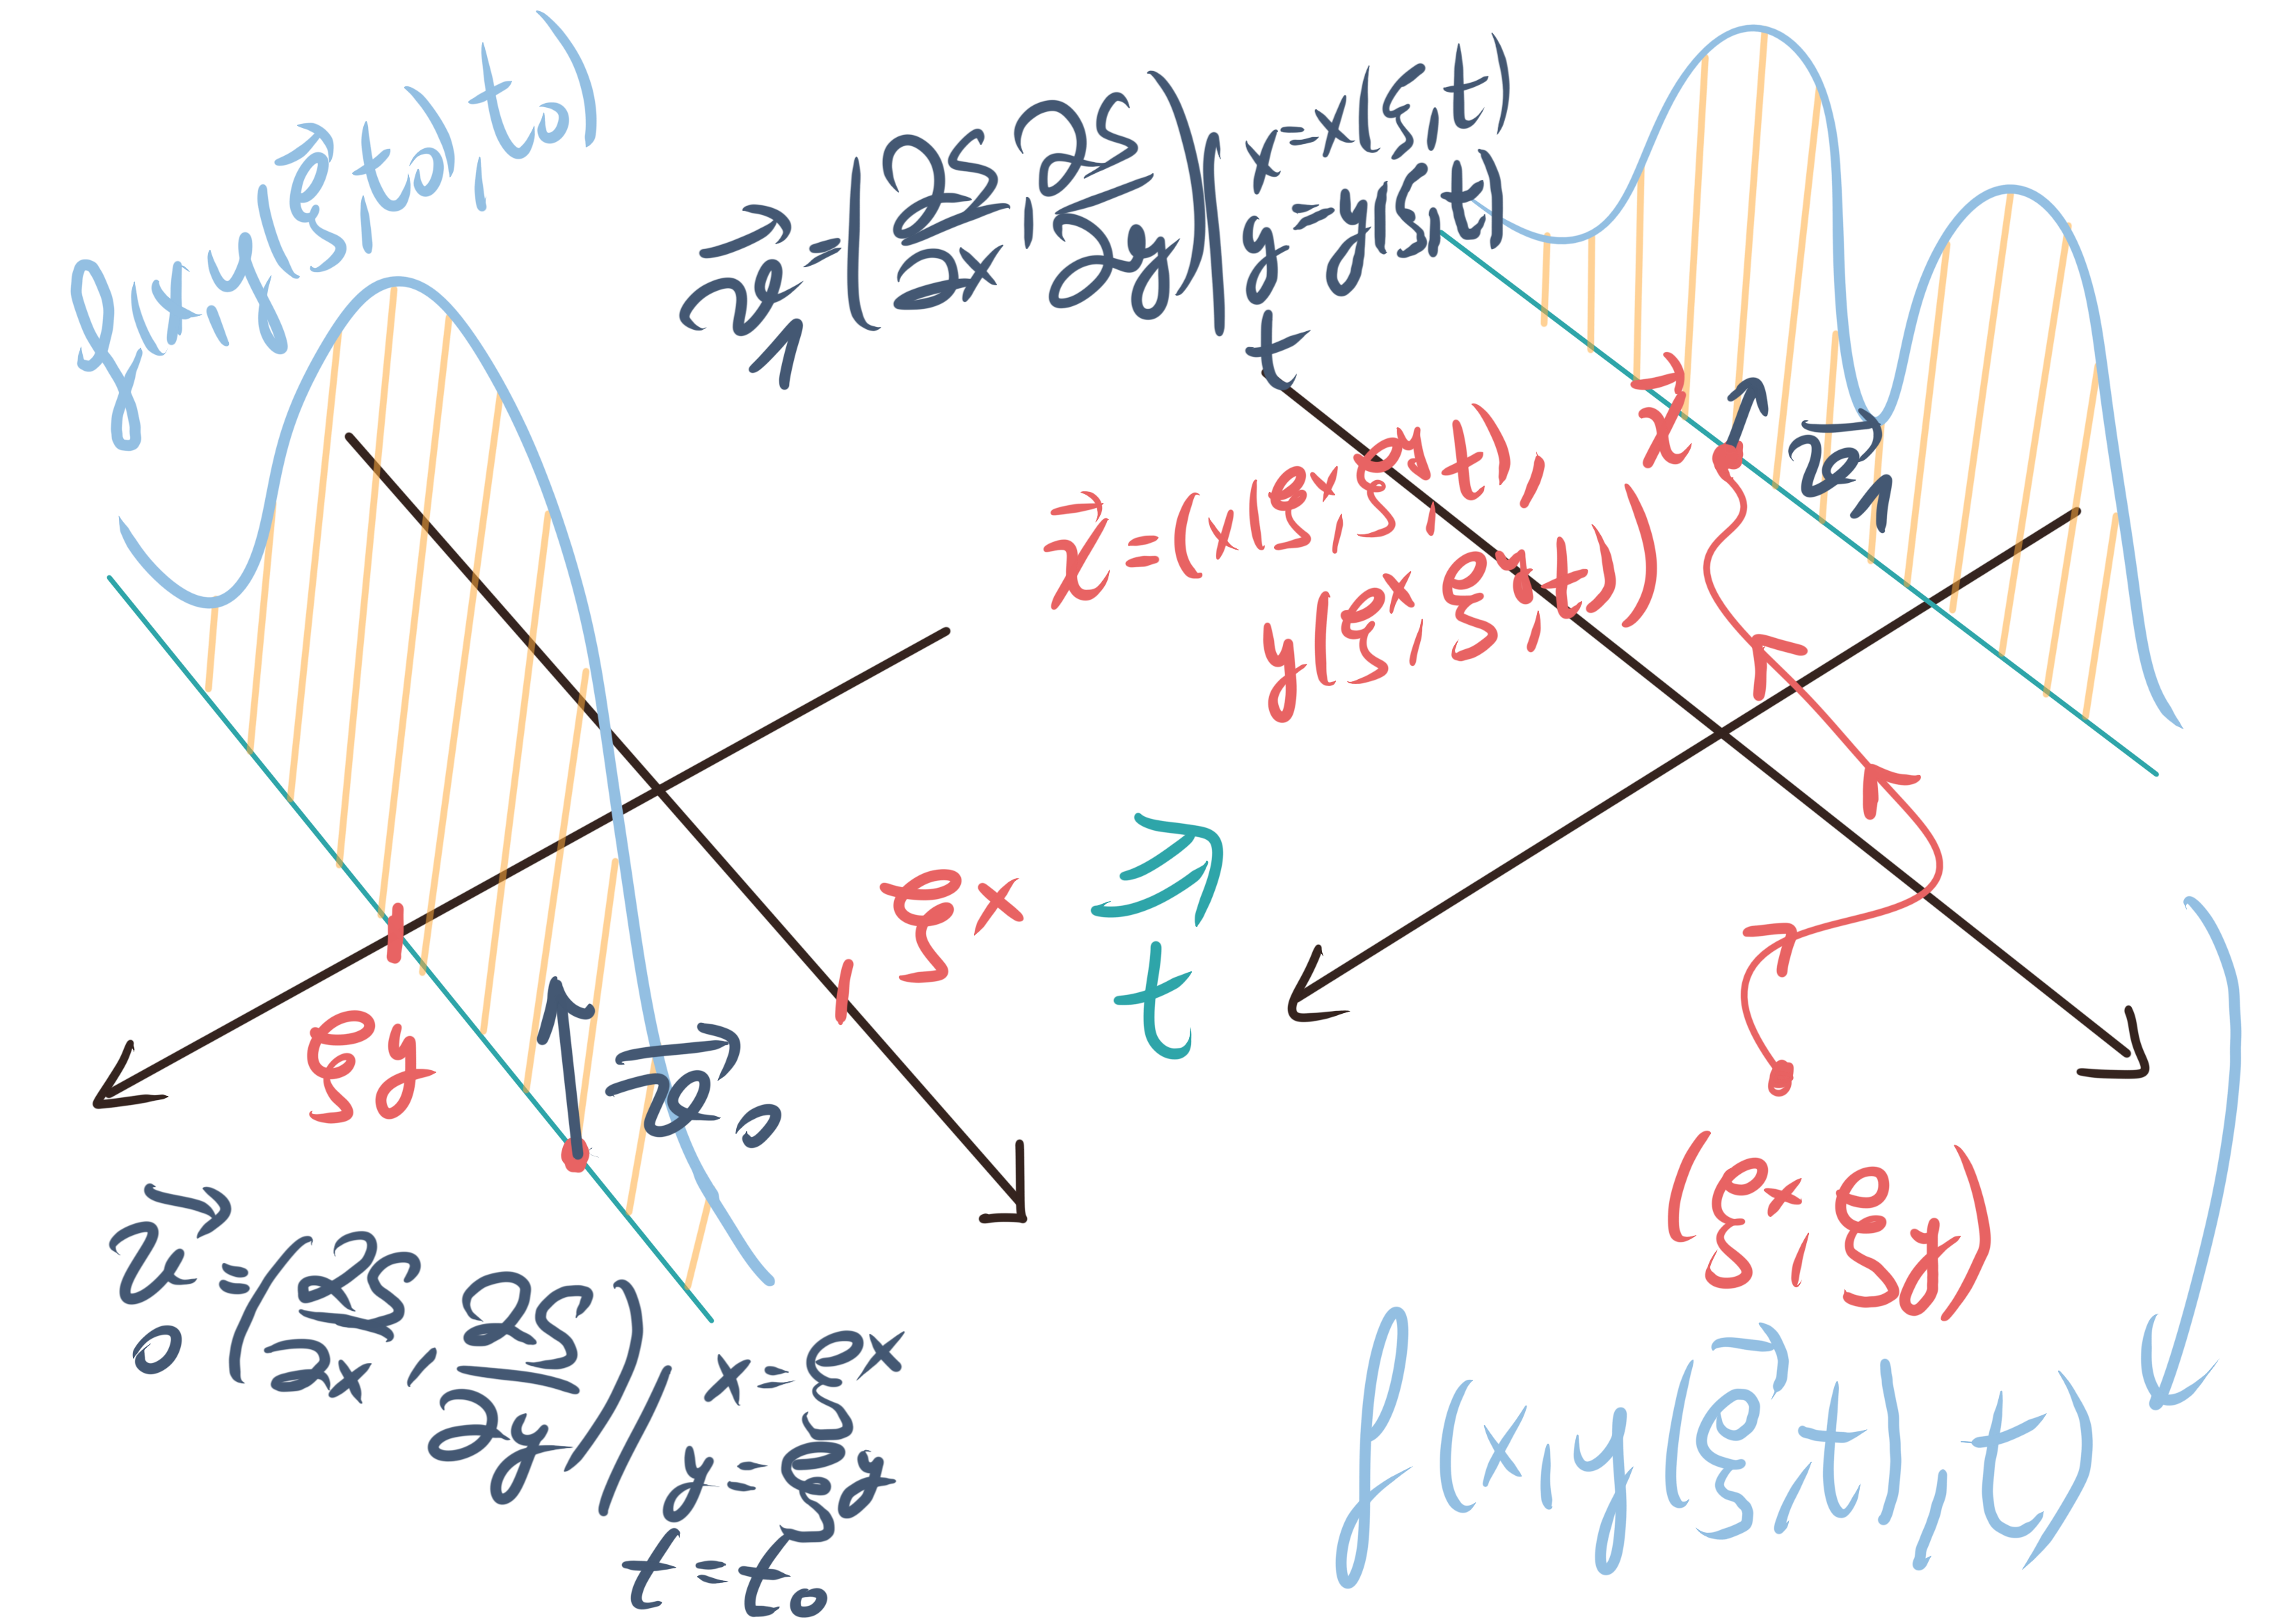
\includegraphics[width=0.64\linewidth]{moving_bohmian.png}
  \caption{A conditional function that is evaluated in $\vec{y}$ along a single Bohmian trajectory. In the left at time $t_0$ and in the right at time $t$ . The velocity with which the slice is moved in $\vec{y}$ is the same for all the Eulerian positions, meaning the initially affine support will be affine at all times. Note that the slice itself always occupies all the domain in $\vec{x}$. It does not move in $\vec{x}$ with the Bohmian trajectory, only in $\vec{y}$. Yet the track in $\vec{x}$ for the Bohmian trajectory is essential for its proper univalued evolution in $\vec{y}$. }
  \label{fig:singleTraj}
\end{figure}

Therefore, for both allowing a homogeneous interpretation of physics and allowing the coupled description of a conditional function with Bohmian trajectories in the full configuration-space (which seem philosophically the most interesting trajectories we can get), we will consider the whole space $\vec{\x}\in\Omega_t\subseteq\R^N$ to be a fluid composed of $N$-dimensional point-like fluid elements, just that we will still consider conditional functions with some Eulerian degrees, for their potential benefits.

For this, we will use $\vec{\xi}_x=(\xi_1,...,\xi_m)$ to denote the implicit Lagrangian labels of the degrees of freedom treated in the Eulerian frame $\vec{x}$, while $\vec{\xi}_y=(\xi_{m+1},...,\xi_N)$ will denote the labels of the explicit Lagrangian degrees of freedom. In general, to uniquely identify a fluid element and its associated conditional function, we will not have enough with $\vec{\xi}_y$, as seen in the boxes, but will require the full label $\vec{\xi}=(\vec{\xi}_x,\vec{\xi}_y)\in \Omega_0\subseteq\R^N$. This means that now the velocity field driving the fluid elements can be dependent on $\vec{x}$. Since we assume the velocity field will be continuous, by the Picard-Lindelöf theorem, there will be a diffeomorphism describing the trajectories for the full system, which we will denote again by $\vec{\x}(\vec{\xi},t)=(\vec{x}(\vec{\xi},t), \vec{y}(\vec{\xi},t))=(\vec{x}^{\, \xi}(t),\vec{y}^{\, \xi}(t))$. 

\subsection*{Complementary Conditional Functions}

Whenever we consider a conditional function $f(\vec{x},\vec{y}(\vec{\xi},t),t)$, since we implicitly assume a trajectory for all the degrees of freedom $(\vec{x}(\vec{\xi},t), \vec{y}(\vec{\xi},t))$, we will also be able to conceive another conditional function "coupled" to the first through the trajectory of the same fluid element $\vec{\xi}$, namely $f(\vec{x}(\vec{\xi},t),\vec{y},t)$. In fact, we could consider several conditional functions, until $N$, each with a different dimensionality, all of which are conditioned to parts of the {\bf same} global trajectory. For example, we could consider the three complementary conditional functions $\{f(x_1(\vec{\xi},t),x_2(\vec{\xi},t),x_3,...,x_N,t)$, $f(x_1, x_2, x_3(\vec{\xi},t), x_4,...,x_N,t), f(x_1, x_2, x_3, x_4(\vec{\xi},t),...,x_N(\vec{\xi},t),t)\}$, where the first one has $N-2$ Eulerian dimensions, the second one has $N-1$ and the third one has three. All of them are orchestrated by the same trajectory $\vec{x}^\xi(t)$.

In general, we will call these conditional functions coupled by parts of the same global trajectory, {\bf complementary conditional functions} (see Figure \ref{fig:complementary} for an intuition).
\vspace{0.3cm}

\begin{figure}[h!]
  \centering
    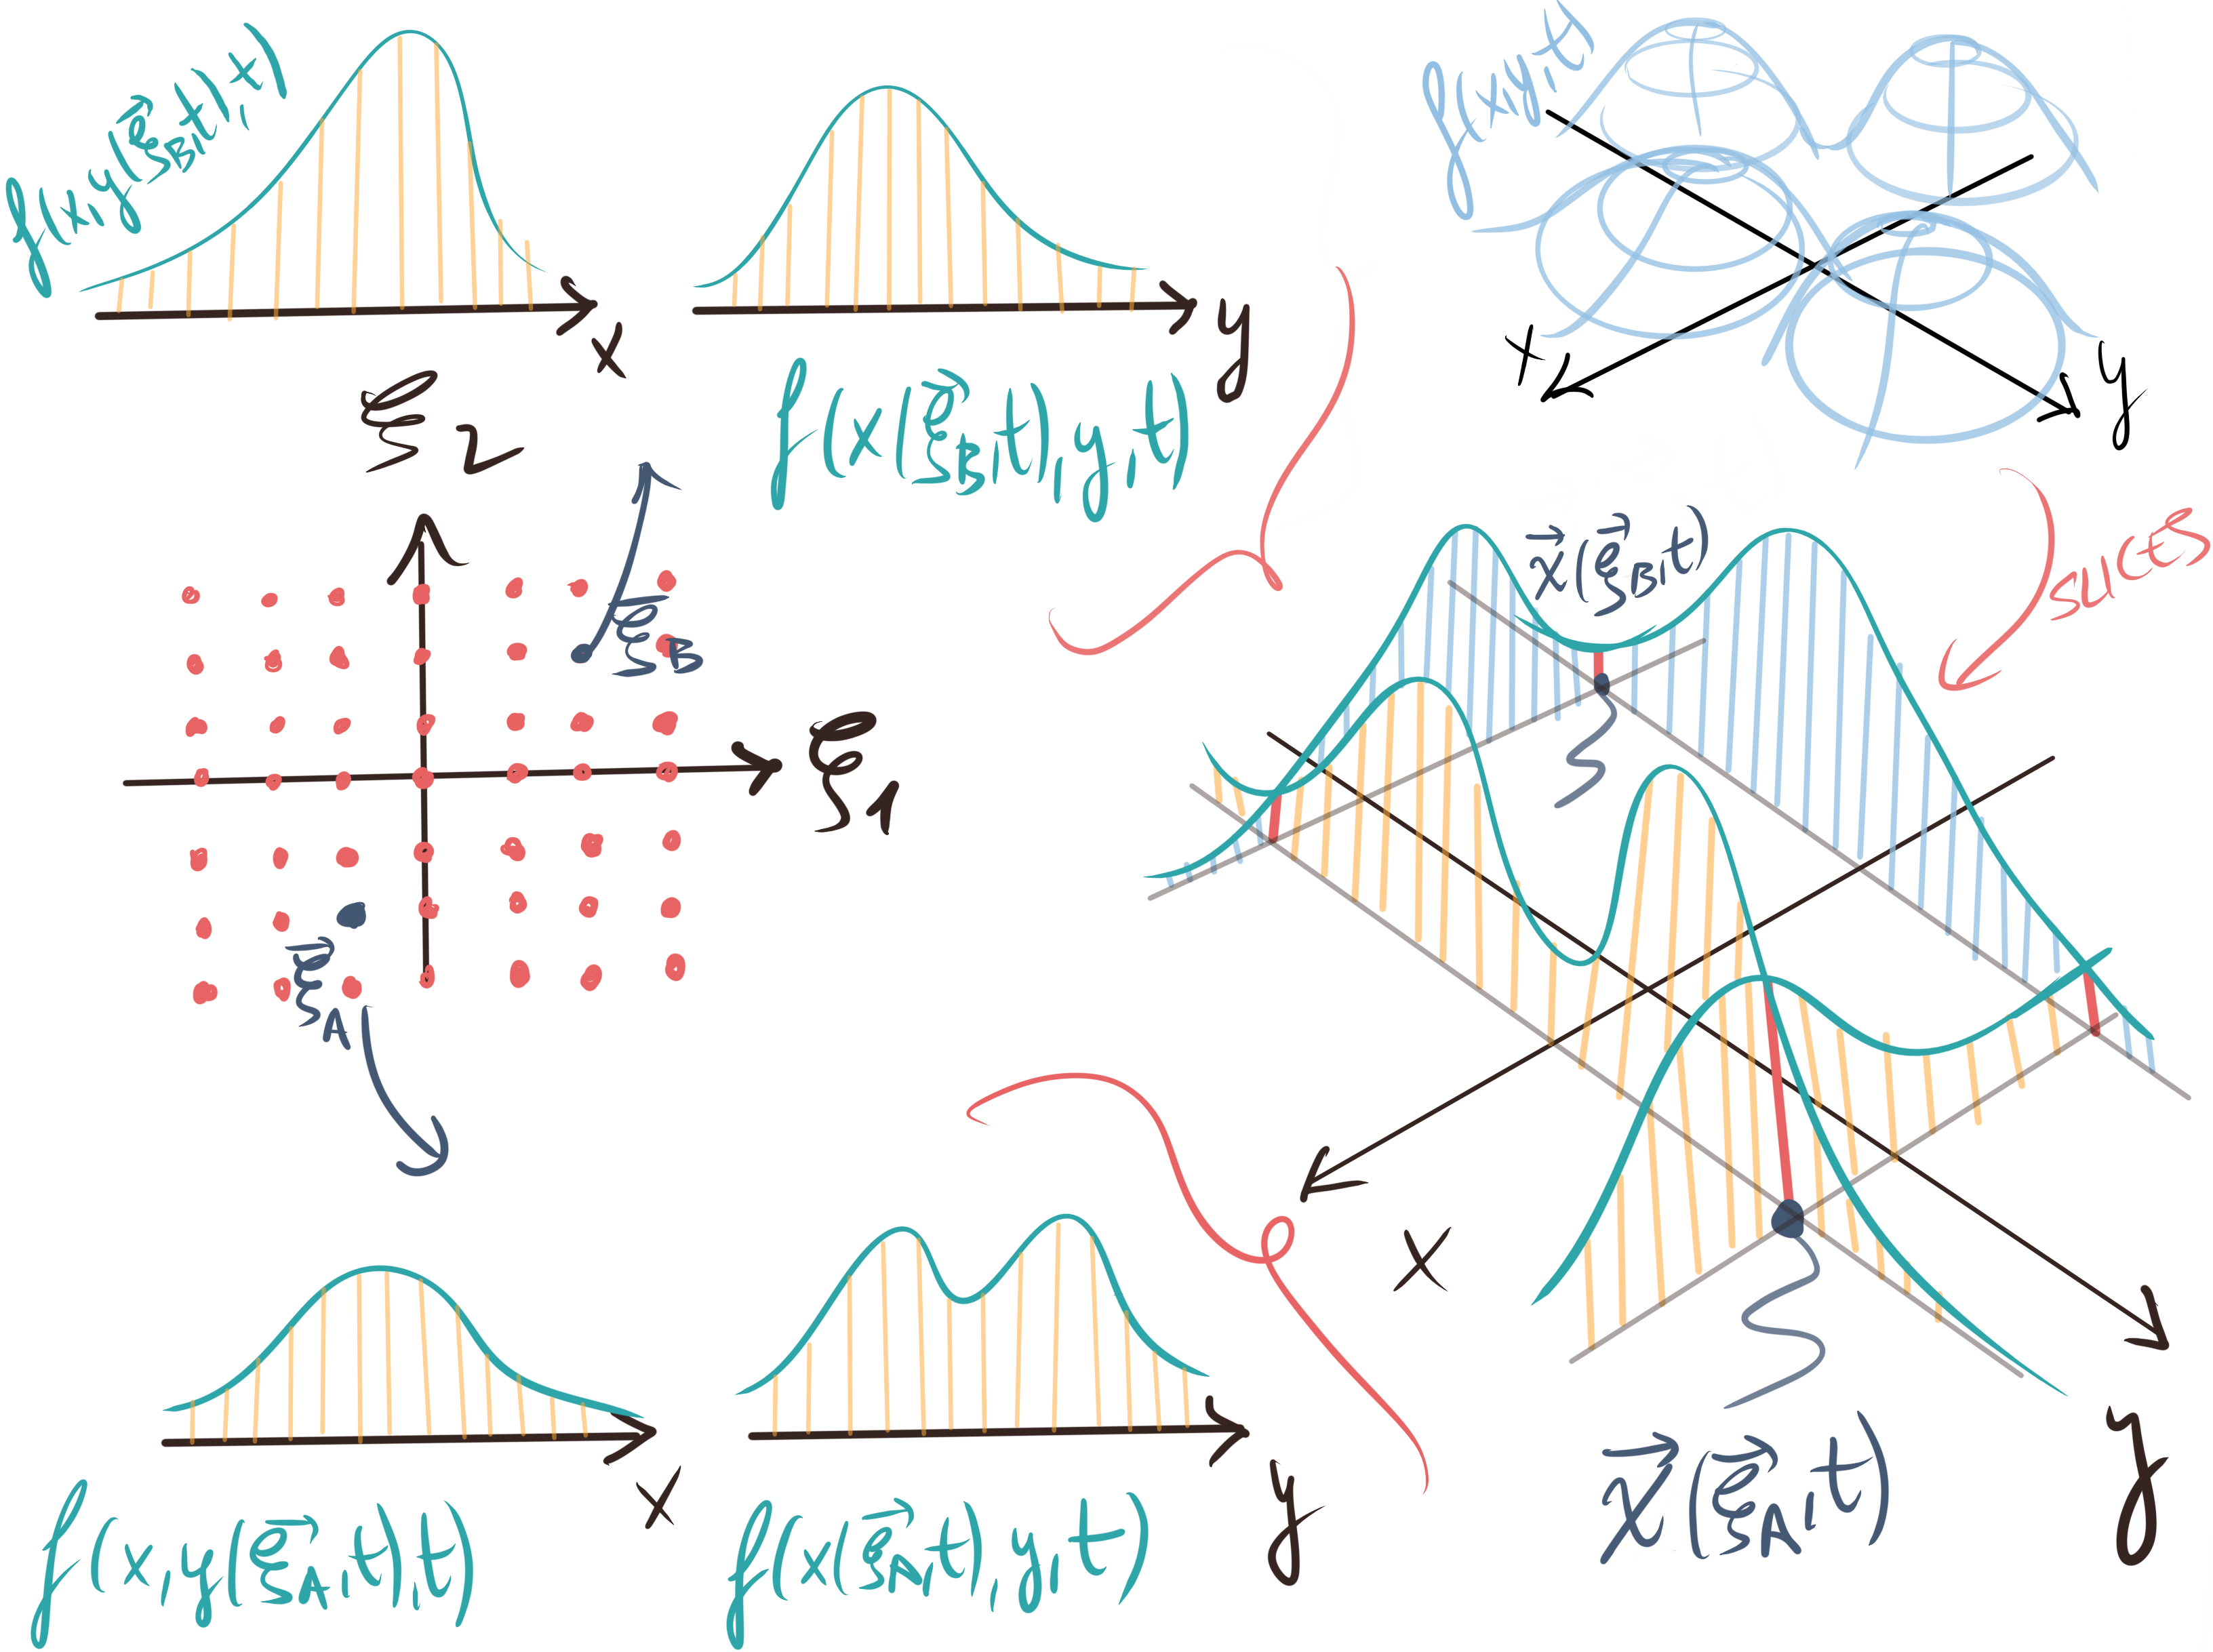
\includegraphics[width=0.75\linewidth]{7slices_complementary.png}
  \caption{ Visual intuition about the complementary conditional functions in $N=2$. In the center left, we see the implicit grid of fluid elements of the whole quantum system. The red dots symbolize each a fluid element we will evolve in time. Each will have its own conditional functions associated, one in $x$ and one in $y$. In the right we see how several of these complementary conditional functions (each set having its trajectory $\vec{\x}(\vec{\xi},t)$) gives us an intuition of the full function $f(x,y,t)$ (in blue above) in terms of crossed slices moving in $\R^N$. Note that in the intersection between the conditional functions of different trajectories, the value of the conditional function should be exactly the same. This could be a numerical indicator of the goodness of the time evolution. }
  \label{fig:complementary}
\end{figure}

Interesting particular cases will be:
\begin{itemize}
\item Having $N$ complementary conditional functions. One per each degree $x_k$. Each conditional function would describe the full function conditioned to the rest of the system being in the given trajectory $f(x_1,x_2^\xi(t),...,x_N^\xi(t),t)$. Meaning that each degree of freedom will be described by a 1D Eulerian function $f(x_k,t;\vec{y}^{\, \xi}(t))$ and a point-like position $x_k(\vec{\xi},t)$.
\item Having $N/3$ complementary conditional functions, one per triad of degrees of freedom. This way, we could have a three Eulerian dimension function describing each three dimensional physical space particle $f(x_k,x_{k+1},x_{k+2},t; \vec{y}^{\, \xi}(t))$ with support exclusively in the physical space coordinates of the particle, together with the 3D position of the particle $(x_{k}(\vec{\xi},t), x_{k+1}(\vec{\xi},t),x_{k+2}(\vec{\xi},))$. $\vec{\xi}$ would reflect the initial position of the particle and the initial position of the rest of the particles in the system and there would be a global trajectory describing the motion of them all. For each possible initial position of the system, we would have a different set of 3D functions and trajectories per particle\footnote{ This suggests a very interesting philosophical understanding of quantum physics, which we will start to discuss in the next section and continue later on. Note however that all these {\bf possible} physical space functions and trajectories for each particle will influence each other contingently even if only one of them is "really existing physically" (they will push each other in configuration-space through the correlation potentials).}.
\item Having 2 complementary conditional functions: one for our lab system and one for the rest of the particles in the Universe (the environment). We would then have a conditional function for the lab system and a conditional function for the environment, both coupled through the common global trajectory of the system.
\end{itemize} 
Hereafter, we will assume when describing a conditional function that along with it, we can also consider the rest of complementary conditional functions associated to its global trajectory.

Note that if we consider a whole set of complementary conditional functions for each fluid element in a given discretized grid of $\R^N$, $\{\vec{\xi}^j\}_{j=1}^M$, we will have that for all the fluid elements that at a certain time turn to be aligned along any $x_k$ axis, their conditional functions in that axis will be exactly the same. See Figure \ref{fig:over} for a visual understanding. This means that we will have an over-representation of the "slices" of the full function. In the numerical/computational approaches, this will not be something to really worry about, since the positions being real numbers makes it is hardly impossible to have more than one trajectory passing from the same $x_k$ point at the same time. However, in theory an infinite amount of trajectories cross the same point in $x_k$ at the same time, which is why we rise up this over-representation warning.\vspace{0.5cm}

\begin{figure}[h!]
  \centering
    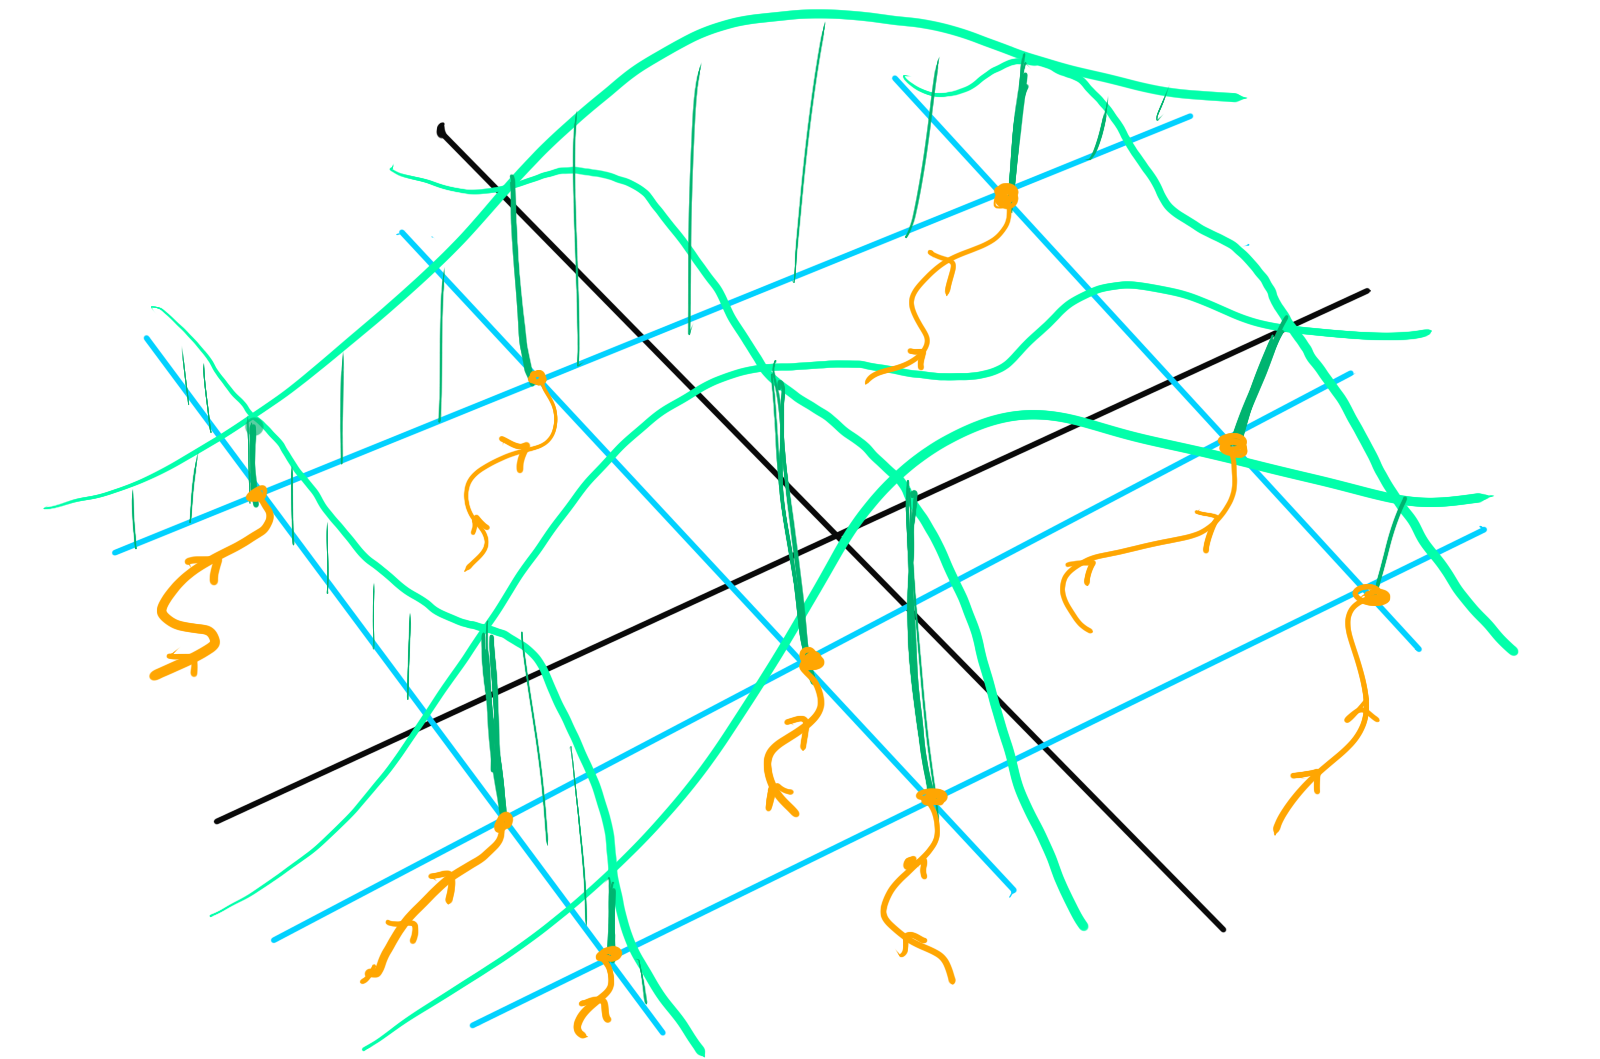
\includegraphics[width=0.65\linewidth]{many_bohmian.png}
  \caption{In blue we can see the affine supports of several pairs of complementary functions. In each intersection we would have enough information as for evolving a Bohmian trajectory. Note that if each intersection represents a Bohmian trajectory with its complementary $x$ and $y$ conditional functions, then all the trajectories that in a certain time turn out to be aligned in any of the blue lines ($x$ or $y$ axes), will have an exactly same conditional function in that axis. This means that their complementary conditional function sets will share a whole function. There is an over-representation of slices of the full function. }
  \label{fig:over}
\end{figure}
\newpage
\subsection*{Why some Bohmian believe the Complementary Conditional Functions and their Trajectory are the {\em arkhe} of the Quantum world?}
There is a very relevant observation from the philosophical standpoint about the complementary conditional wavefunctions of a certain global trajectory. Following the Bohmian velocity fields \eqref{v}, the velocity piloting the movement of the trajectory, in any Eulerian axis $x_k$, only depends on the derivative of the action in that same direction $\pdv{}{x_k}$ evaluated at the current position of the trajectory. This means that we have enough with a set of complementary conditional wavefunctions (say $\psi(\vec{x},\vec{y}(\vec{\xi},t),t)$ and $\psi(\vec{x}(\vec{\xi},t),\vec{y},t)$) in order to know the velocity of the trajectory in all the $N$ directions, since these conditional functions give us the variation of the full function exactly in the directions and positions we need. We have enough with these slices, as can be seen depicted in Figure \ref{fig:pair_bohm}. This suggests that if the Bohmian trajectory of the system is the ultimate reality, since the complementary conditional functions (the wavefunction or the action and density) of a certain trajectory are the only necessary functions to predict its motion, then there must be some serious weight in those complementary conditional functions. 

\begin{figure}[h!]
  \centering
    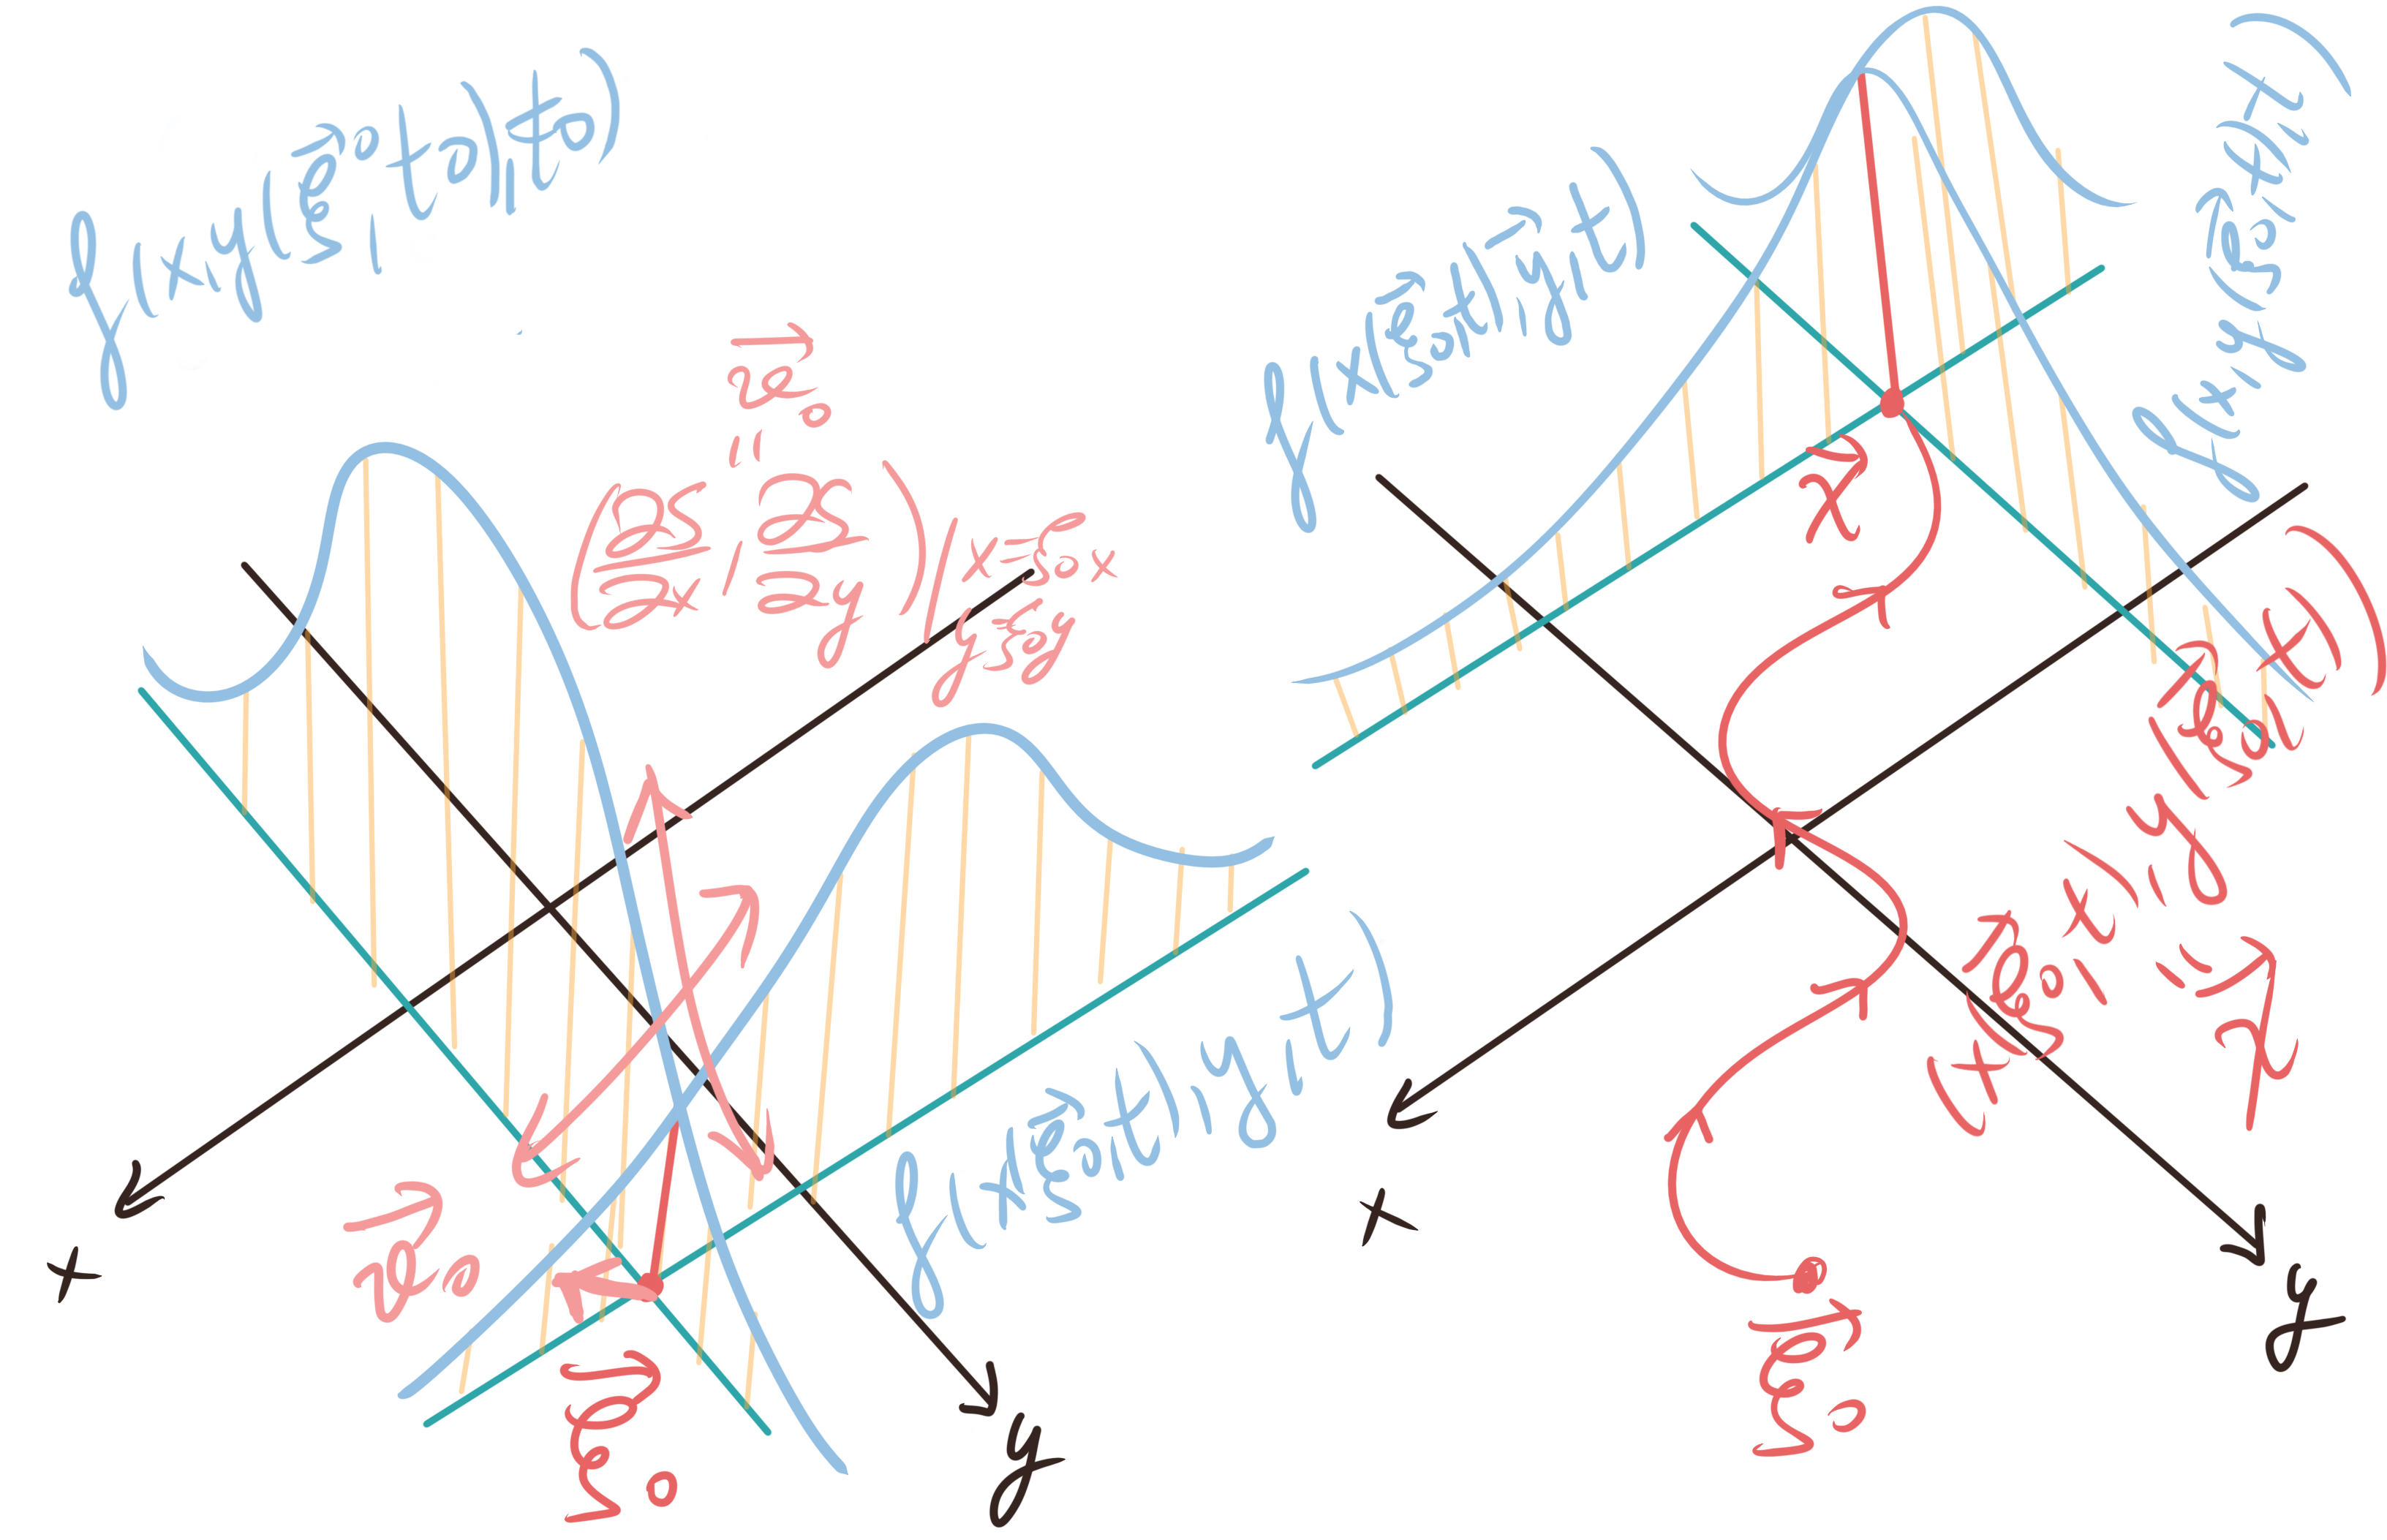
\includegraphics[width=0.65\linewidth]{bohmian_pair.png}
  \caption{Following the same caption of Figure \ref{fig:singleTraj}, we see that having a pair of complementary functions, where one of them has as Lagrangian degrees of freedom the Eulerian ones of the other, gives us all the information we need to evolve the Bohmian trajectory to the next time step. The velocity of the Bohmian trajectory is the partial derivative in $x$ and in $y$ of the full function, just over the position of the trajectory, which is precisely the information provided by the complementary slices (in pink). }
  \label{fig:pair_bohm}
\end{figure}

It is however somewhat fallacious to say this, since as we will see, the equations that predict the motion of those complementary conditional functions, the only things affecting the trajectory, actually depend on the rest of (possible) complementary conditional functions. This will be because their time evolution will require the knowledge of the derivatives $\pdv{}{x_k}$ on the Lagrangian axes, for all the Eulerian positions $\vec{x}$ of the slice. Since we are considering with each conditional function a single slice, we will not have enough information. We will have this information at the exact point of the trajectory $\vec{\x}^\xi(t)$, thanks to the complementary conditional functions (which is why we can evolve the Bohmian trajectory), but not in all the rest of Eulerian positions of any of the complementary conditional functions. And we need this to evolve them as a whole. Thus, while it is true that we do not need the full function (or equivalently, the rest of slices), to evolve the Bohmian trajectory, we still do need them to evolve the complementary conditional functions themselves.

We will see in section (II.h) however, a formidable way to hide this dependency and actually make the complementary conditional functions a possible ontological basis of reality. We will then realize that this has actually big epistemological importance.

\newpage


\section*{(III.a) The Schrödinger Equation}
\addcontentsline{toc}{subsubsection}{{\bf (III.a)} The Schrödinger Equation}
The Schrödinger Equation \eqref{SE} will provide us after some manipulation, some equations to predict the time evolution of the conditional wavefunctions. The resulting equations will turn out to depend on variations of the functions in the Lagrangian axes $\vec{y}$, meaning the evolution of each conditional function will depend on the rest of adjacent possible conditional functions (the rest of slices of the full function). In general we will call the terms correlating the conditional functions, {\bf correlation terms}.
\subsection*{(III.a.1) Kinetic and Advective Correlation Terms}
%\addcontentsline{toc}{subsubsection}{{\bf (III.a.1)} The Schrödinger Equation: Kinetic and Advective Correlation Terms}
If we evaluate $\vec{y}=\vec{y}(t,\vec{\xi})$ in the Schrödinger Equation \eqref{SE}, leaving $\vec{x}$ in the Eulerian frame, we get:
\begin{equation}
i\hbar \pdv{}{t}\psi(\vec{x}, \vec{y}^{\, \xi}(t),t)=-\sum_{j=1}^m \frac{\hbar^2}{2m_j}\pdv[2]{}{x_j} \psi(\vec{x}, \vec{y}^{\, \xi}(t),t) + U(\vec{x}, \vec{y}^{\, \xi}(t),t)\psi(\vec{x}, \vec{y}^{\, \xi}(t),t) -\sum_{j=m+1}^N \frac{\hbar^2}{2m_j}\pdv[2]{}{x_j} \psi(\vec{x}, \vec{y},t)\Big\rvert_{\vec{y}^{\, \xi}(t)}
\end{equation}
Then, since by the chain rule:
\begin{equation}
\dv{}{t}\psi(\vec{x}, \vec{y}^{\, \xi}(t),t)=\pdv{}{t}\psi(\vec{x}, \vec{y}^{\, \xi}(t),t)+\sum_{j=m+1}^N \pdv{}{x_j}\psi(\vec{x}, \vec{y},t)\Big\rvert_{\vec{y}^{\, \xi}(t)}\cdot \pdv{x_j(\vec{\xi},t)}{t}
\end{equation}
We get the following equation ruling the motion of the conditional wavefunctions:
\begin{equation}\label{KinAdvEL}
i\hbar \dv{}{t}\psi(\vec{x}, \vec{y}^{\, \xi}(t),t)=\qty[-\sum_{j=1}^m \frac{\hbar^2}{2m_j}\pdv[2]{}{x_j} + U(\vec{x}, \vec{y}^{\, \xi}(t),t)]\psi(\vec{x}, \vec{y}^{\, \xi}(t),t)+K(\vec{x}, \vec{y}^{\, \xi}(t),t)+A(\vec{x}, \vec{y}^{\, \xi}(t),t)
\end{equation}

Where we define the so called {\bf Kinetic and Advective correlation terms}:
\begin{equation}\label{KinEL}
K(\vec{x}, \vec{y}^{\, \xi}(t),t):=-\sum_{j=m+1}^N \frac{\hbar^2}{2m_j}\pdv[2]{}{x_j} \psi(\vec{x}, \vec{y},t)\Big\rvert_{\vec{y}^{\, \xi}(t)}
\end{equation}
\begin{equation}\label{AdvEL}
A(\vec{x}, \vec{y}^{\, \xi}(t),t):=i\hbar\sum_{j=m+1}^N \pdv{}{x_j}\psi(\vec{x}, \vec{y},t)\Big\rvert_{\vec{y}^{\, \xi}(t)}\cdot \pdv{x_j(\vec{\xi},t)}{t}
\end{equation}
Equation \eqref{KinAdvEL}, ruling the motion of the conditional wavefunctions $\psi(\vec{x}, \vec{y}^{\, \xi}(t),t)$ is almost a Schrödinger Equation for a system of $m$ (instead of $N$) dimensions. The difference is that we now have two additional affine terms in the equation, that actually depend on derivatives of the full wavefunction in the axes that we are considering in the Lagrangian frame. As we already anticipated that would happen, if we want to evolve a single conditional wavefunction (or the complementary conditional wavefunction set it is part of), we do not have enough with themselves. We would require the knowledge of complementary conditional wavefunctions of other nearby trajectories. It is just the same problem that we faced with the fully Lagrangian picture. As such, to solve this problem we will be able to use the same strategies: 
\begin{enumerate}
\item[($\alpha$)] Evolve several trajectories and their conditional wavefunctions and use them as a discretized version of the full wavefunction to get the derivatives for each trajectory. We would have the problem that the grid would become non-equispaced (like in the fully Lagrangian case), even if the unstructuring in this case would be better behaved, since each single conditional function already gives us a whole set of structured (Eulerian) points occasionally.

To face the derivatives in the Lagrangian axes in this unstructured grid, among others, we could:
\begin{enumerate}
\item Change the derivatives in $x_k$ to derivatives in the label space $\xi_k$, which we could choose to be equi-spaced.
\item Fit a sum of analytic functions and compute the derivatives symbolically.
\item Use a $K$ nearest neighbour approach to predict the full wavefunction and make numerical derivatives.
\end{enumerate}

\item[($\beta$)] Evolve the derivatives of the wavefunction along the trajectories, using a chain of infinite differential equations. Similarly, one could evolve the Kinetic and Advective correlation potentials themselves in time.
\end{enumerate}
%Klaro figura honen pblmie da ke en N mas grnades no tienen porke kedar alineados los cwf differentes asike pf no es tan inmediato
%\begin{figure}[h!]
 % \centering
 %   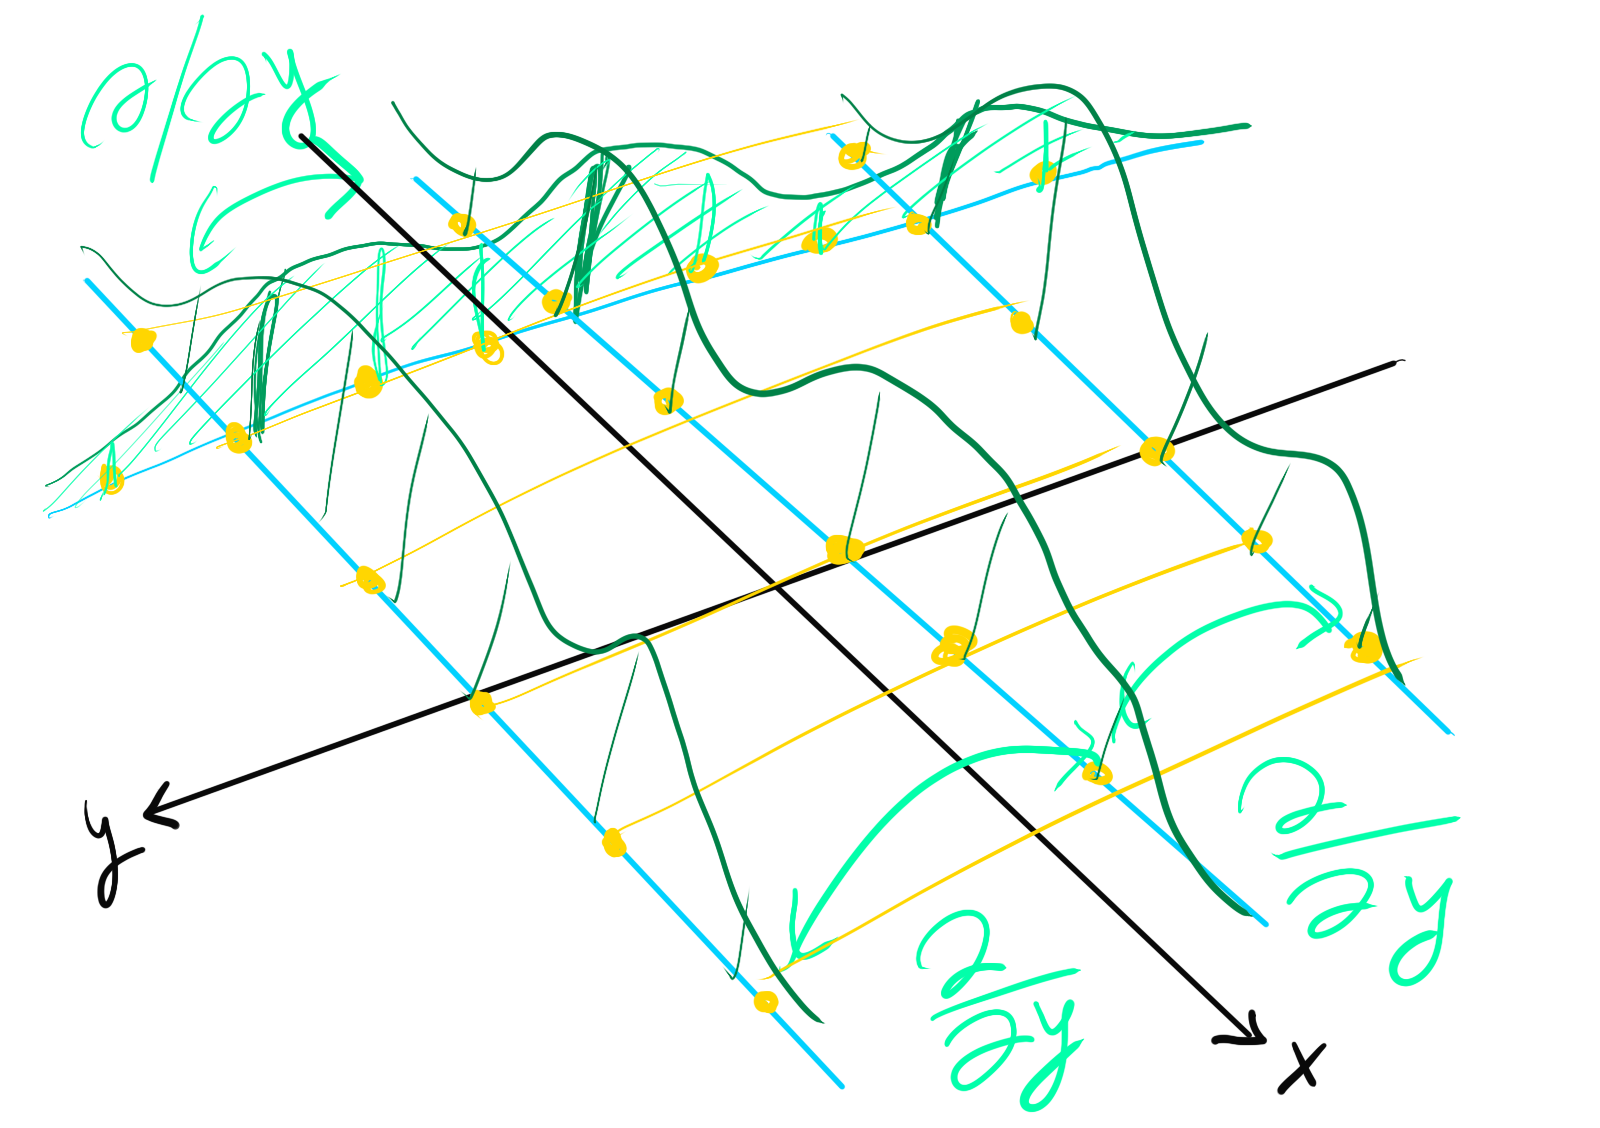
\includegraphics[width=0.65\linewidth]{aligned_original.png}
%  \caption{Depiction of several complementary conditional functions. The yellow dots show the discrete elements of the Eulerian degrees of each conditional function. This image shows two things: 1. parallel conditional functions (conditional functions with the same Lagrangian degrees but different initial trajectory positions) can be used to approximate derivatives in the Lagrangian directions $\pdv{}{y}$. 2. Crossed CWF-s with complementary Lagrangian degrees can be used also to approximate derivatives in the Lagrangian directions with a higher degree of precision than using parallel CWF-s.  }
%  \label{fig:aligned2}
%\end{figure}


\subsection*{(III.a.2) G and J Correlation Potentials}
%\addcontentsline{toc}{subsubsection}{{\bf (III.a.2)} The Schrödinger Equation: G and J Correlations}
In this section we will develop a Schrödinger-like equation for the conditional wavefunctions that this time will at least resemble to be linear, unlike the Kinetic and Advective equation \eqref{KinAdvEL}.

Following the development in Chapter 1 of \cite{JordiXO}, an arbitrary non-zero and single valued complex function $f(\vec{x}, t):\R^m \rightarrow \C$ can be imposed to be the solution of an m dimensional Schrödinger equation:
\begin{equation}
i \hbar \pdv{f(\vec{x},t)}{t} = -\sum_{k=1}^m\frac{\hbar^2}{2 m_k}\pdv[2]{f(\vec{x},t)}{x_k} + W(\vec{x},t) f(\vec{x},t)
\end{equation}
if the potential term $W(\vec{x}, t)$ is defined as:
\begin{equation}
W(\vec{x}, t) := \qty(i \hbar \pdv{f(\vec{x},t)}{t} +\sum_{k=1}^m\frac{\hbar^2}{2 m_k}\pdv[2]{f(\vec{x},t)}{x_k} ) \frac{1}{f(\vec{x},t)}
\end{equation}
The proof is immediate. An observation that we must note is that for an arbitrary $f(\vec{x},t)$, the potential $W(\vec{x},t)$ can be complex, which was not the case in the usual Schrödinger Equation.

If we now take the conditional wavefunction,  and write it in polar form: $\psi(\vec{x}, \vec{y}^{\, \xi}(t),t)=:\psi^\xi (\vec{x},t)=\p^\xi(\vec{x},t) e^{i\z^\xi(\vec{x},t) / \hbar}$, by introducing it in $W^\xi(\vec{x},t)$ we will get what the complex potential should be for the conditional wavefunction to be ruled by a Schrödinger-like equation:
\begin{equation}\label{Wxi}
W^\xi(\vec{x}, t) = -\sum_{k=1}^m\frac{1}{2m_k} \qty( \qty(\pdv{\z^\xi}{x_k})^2 -\frac{\hbar^2}{\p^\xi}\pdv[2]{\p^\xi}{x_k})\ -\pdv{\z^\xi}{t}+ \ i \ \frac{\hbar}{\p^{\xi\ 2}} \qty(\pdv{\p^{\xi\ 2}}{t}+\sum_{k=1}^m\pdv{}{x_k}\qty(\frac{\p^{\xi\ 2}}{m_k}\pdv{\z^\xi}{x_k}))
\end{equation}
where we used the Leibniz derivative rule and an inverse chain rule. Note that the potential term depends on the trajectory we choose. In general we will use $:=\W(\vec{x},\vec{y}^{\, \xi}(t),t):=W^\xi(\vec{x},t)$.
%Separating the real and imaginary parts:
%$$
%\begin{cases}
%\mathbb{R}e\{W(\vec{x},t)\}=-\pdv{\z^\xi(\vec{x},t)}{t}-\frac{1}{2m_a} \qty( \qty(\pdv{\z^\xi(\vec{x},t)}{x_a})^2 -\frac{\hbar^2}{\p^\xi(\vec{x},t)}\pdv[2]{\p^\xi(\vec{x},t)}{x_a})\vspace{-0.3cm} \\ \\
%\mathbb{I}m\{W(x_a, t)\} = \frac{\hbar}{\p^\xi(\vec{x},t)^2} \qty(\pdv{\p_a^2}{t}+\pdv{}{x_a}\qty(\frac{\p_a^2}{m_a}\pdv{\z_a}{x_a}))\vspace{-0.1cm}
%\end{cases}
%$$
%Where we can recognize the \ref{QHJE} for a single particle in 1D. As such, the real part of W is simply the scalar real potential, then the Hamiltonian, followed by the kinetic energy and the quantum potential of a 1D particle.
%Which is clearly a modified particle conservation equation \ref{CE}. Note how if  $Im\{W(x_a, t)\} =0$ then we get the common continuity equation, which would mean that probability is conserved, and the solution $\Phi(\vec{x},t)$ would preserve its norm at all times (the conditional $r_a^2$ would integrate a same norm at all times in its spatial dimension $x_a$). Nonetheless, if $Im\{W(x_a, t)\} \neq 0$, then particles/probability are NOT conserved, and their source or sink will be quantified by $\frac{2 \_a^2}{\hbar} Im\{W(x_a, t)\}$. Therefore, the norm of $\psi^\xi (\vec{x},t)$ will not need to be preserved in the time evolution. \vspace{-0.3cm}\\

%If $W^\xi$ has that shape, $\psi^\xi (\vec{x},t)$ will be the solution of the $m$ dimensional Schrödinger-like Equation:\vspace{-0.2cm}
%$$
%i \hbar \pdv{\psi^\xi (\vec{x},t)}{t} = -\sum_{k=1}^m \frac{\hbar^2}{2 m_k}\pdv[2]{\psi^\xi (\vec{x},t)}{x_k} + W^\xi(\vec{x},t) \psi^\xi (\vec{x},t)\vspace{-0.2cm}
%$$
%which if $\mathbb{I}m\{W^\xi\} =0$ would look like an actual mD Schrödinger Equation. However, $W^k$ depends on parts of the CWF itself, so the differential equation is  {\bf non-linear} even in that case.

Using that $\psi^\xi ( \vec{x}, t) := \Psi(\vec{x}, \vec{y}^{\, \xi}(t),t)$ means that $\z^\xi(\vec{x},t)=S(\vec{x}, \vec{y}^{\, \xi}(t),t)$ and $\p^\xi (\vec{x},t)=R(\vec{x}, \vec{y}^{\, \xi}(t),t)$, where we have that the full wavefunction in polar form is $\Psi(\vec{x},\vec{y},t)=R(\vec{x},\vec{y},t)e^{iS(\vec{x},\vec{y},t)/\hbar}$, applying the chain rule, the real part of $W^\xi(\vec{x},t)$ yields:
\begin{equation}
\R e\{\W(\vec{x}, \vec{y}^{\, \xi}(t),t)\}=
\sum_{a=1}^m \Big\{-\frac{1}{2m_a} \qty(\pdv{S(\vec{x}, \vec{y}^{\, \xi}(t),t)}{x_a})^2 +\frac{\hbar^2}{2m_aR(\vec{x},\vec{y}^{\, \xi}(t),t)}\pdv[2]{R(\vec{x}, \vec{y}^{\, \xi}(t),t)}{x_a}\Big\}-\dv{S(\vec{x},\vec{y}^{\, \xi}(t),t)}{t}=
\end{equation}
$$
\sum_{a=1}^m\Big\{-\frac{1}{2m_a} \qty(\pdv{\z^\xi(\vec{x},t)}{x_a})^2 +\frac{\hbar^2}{2m_a\p^\xi(\vec{x},t)}\pdv[2]{\p^\xi(\vec{x}, t)}{x_a}\Big\}- \ \qty(\pdv{S(\vec{x},\vec{y},t)}{t}\Big\rvert_{\vec{y}^{\, \xi}(t)}+\sum_{k=m+1}^N \pdv{S(\vec{x},\vec{y},t)}{x_k}\Big\rvert_{x_k^\xi(t)} \dv{x_k^\xi(t)}{t})
$$

Now, knowing that the action follows the Quantum Hamilton-Jacobi Equation \eqref{HJE}, we can evaluate it in place of $-\pdv{S(\vec{x},\vec{y},t)}{t}$ to get:
\newpage
\begin{equation}
Re\{\W(\vec{x}, \vec{y}^{\, \xi}(t),t)\}=\sum_{a=1}^m\Big\{-\frac{1}{2m_a} \qty(\pdv{\z^\xi(\vec{x},t)}{x_a})^2 +\frac{\hbar^2}{2m_a\p^\xi(\vec{x},t)}\pdv[2]{\p xi(\vec{x}, t)}{x_a}\Big\}-
\end{equation}
$$
-\sum_{k=m+1}^N \qty( \pdv{S(\vec{x},\vec{y},t)}{x_k}\Big\rvert_{x_k^\xi(t)} \dv{x_k^\xi(t)}{t})\ + \sum_{k=1}^N \qty[\frac{1}{2m_k} \qty(\pdv{S}{x_k}\Big\rvert_{\vec{y}^{\, \xi}(t)})^2 -\frac{\hbar^2}{2m_kR}\pdv[2]{R}{x_k}\Big\rvert_{\vec{y}^{\, \xi}(t)} ] + V(\vec{x}, \vec{y}^{\, \xi}(t),t)
$$
Observe that in the last sum, the $k=a$ terms are equal to the two initial terms, which cancel each other out and we are left with the final expression:\vspace{-0.1cm}\label{ReW}
\begin{equation*}
\R e\{\W(\vec{x}, \vec{y}^{\, \xi}(t),t)\}= \sum_{k=m+1}^N \qty[\frac{1}{2m_k} \qty(\pdv{S}{x_k}\Big\rvert_{\vec{y}^{\, \xi}(t)})^2 -\frac{\hbar^2}{2m_kR}\pdv[2]{R}{x_k}\Big\rvert_{\vec{y}^{\, \xi}(t)} -\pdv{S}{x_k}\Big\rvert_{x_k^\xi(t)} \dv{x_k^\xi(t)}{t} ] + U(\vec{x}, \vec{y}^{\, \xi}(t),t)
\end{equation*}
We now have re-expressed $\R e(W^\xi)$ without using $\psi^\xi(\vec{x},t)$ to compute it. Instead the dependence on the derivatives in the Lagrangian axes has explicitly emerged. Essentially we can recognize in this potential the kinetic energy of the Lagrangian axes and their quantum potentials. The real part of $W^\xi$ also includes the classical conditional potential $U^\xi$, which introduces the geometric constraints between the Eulerian coordinates as a function of the position of the Lagrangian parts. 

Let us define the part introducing the correlations between the different conditional functions as the {\bf correlation potential $G$}:
\begin{equation}\label{G}
G(\vec{x}, \vec{y}^{\, \xi}(t),t):=  \sum_{k=m+1}^N \qty[\frac{1}{2m_k} \qty(\pdv{S}{x_k}\Big\rvert_{\vec{y}^{\, \xi}(t)})^2 -\frac{\hbar^2}{2m_kR}\pdv[2]{R}{x_k}\Big\rvert_{\vec{y}^{\, \xi}(t)} -\pdv{S}{x_k}\Big\rvert_{x_k^\xi(t)} \pdv{x_k(\vec{\xi},t)}{t} ]
\end{equation}
We could further define each of the summands as $G_k(\vec{x},\vec{y}^{\, \xi}(t),t)$, for a matter of organization, since each summand encapsulates the correlation with the $x_k$ Lagrangian degree.

Performing the same development for the imaginary part of $W^\xi$ in \eqref{Wxi}: evaluating the conditional function in $\mathbb{I}m\{W^\xi(\vec{x},t)\}$ and applying the chain rule, we get:
\begin{equation}
\hspace{-0.7cm}Im\{\W(\vec{x}, \vec{y}^{\, \xi}(t),t)\}=\frac{\hbar}{2R^2}\Big\rvert_{\vec{y}^{\, \xi}(t)} \qty( \pdv{R(\vec{x},\vec{y},t)^2}{t}\Big\rvert_{\vec{y}^{\, \xi}(t)} + \sum_{k=m+1}^N \pdv{R^2}{x_k}\Big\rvert_{\vec{y}^{\, \xi}(t)} \dv{x_k^\xi(t)}{t} + \sum_{a=1}^m\Big\{\pdv{}{x_a} \qty(\frac{R^2}{m_a} \pdv{S(\vec{x}, \vec{y}^{\, \xi}(t),t)}{x_a} ) \Big\})
\end{equation}

As the full density must follow the continuity equation of the configuration-space fluid \eqref{CE}, evaluating it at $\pdv{R(\vec{x},\vec{y},t)^2}{t}$, we will notice there is a cancellation of the $k=a$ terms (as happened with the real part). We then arrive at an expression of the imaginary part, which we will call the {\bf correlation potential $J$}, that is, $J(\vec{x}, \vec{y}^{\, \xi}(t),t):=\mathbb{I}m\{\W(\vec{x}, \vec{y}^{\, \xi}(t),t)\}$, which is given by:
\begin{equation}\label{J}
J(\vec{x}, \vec{y}^{\, \xi}(t),t):= \frac{\hbar}{2R^2}\Big\rvert_{\vec{y}^{\, \xi}(t)} \sum_{k=m+1}^N \qty[ \pdv{R^2}{x_k}\Big\rvert_{\vec{y}^{\, \xi}(t)} \pdv{x_k(\vec{\xi},t)}{t} - \frac{1}{m_k} \pdv{}{x_k} \qty(R^2 \pdv{S}{x_k} )\Big\rvert_{\vec{y}^{\, \xi}(t)} ]
\end{equation}
This is a correlation term as well, because it also depends on derivatives of $R$ and $S$ in the directions of the Lagrangian axes. A complex potential in the Schrödinger Equation makes the evolution be not necessarily unitary, so this potential will account for the variations of the norm of the conditional wavefunction. This norm variation is due to the displacement of the Lagrangian part's trajectory and the movement of the slice along the overall fluid. Once again, we can encapsulate all the summands concerning spatial variations of the Lagrangian degree of freedom $x_k$ in a sub-potential $J_k$. 

With all, we have that the complex potential ruling the motion of the conditional wavefunction $\psi(\vec{x},\vec{y} xi(t),t)$ is decomposed in the following terms:
\begin{equation}
W^\xi(\vec{x},t)=\W(\vec{x}, \vec{y}^{\, \xi}(t),t)= V(\vec{x}, \vec{y}^{\, \xi}(t),t) + \sum_{k=m+1}^N\Big\{ G_k(\vec{x}, \vec{y}^{\, \xi}(t),t)+i\ J_k(\vec{x}, \vec{y}^{\, \xi}(t),t)\Big\}
\end{equation}
Then the conditional wavefunction is ruled in time by:
\begin{equation}\label{SE.GJ}
i \hbar \pdv{\psi^\xi (\vec{x},t)}{t} = \qty[\sum_{a=1}^m\frac{\hbar^2}{2m_a} \pdv[2]{}{x_a} +  U(\vec{x}, \vec{y}^{\, \xi}(t),t) + G(\vec{x}, \vec{y}^{\, \xi}(t),t)+i\ J(\vec{x}, \vec{y}^{\, \xi}(t),t)] \psi^\xi (\vec{x},t)
\end{equation}
which is an $m$ dimensional Schrödinger-like Equation.

Note that there is a functional relationship between the Kinetic and Advective correlation terms \eqref{KinEL} and \eqref{AdvEL}, and the $G$ and $J$ correlation potentials we just described: 
\begin{equation}
\qty(G(\vec{x}, \vec{y}^{\, \xi}(t),t)+iJ(\vec{x}, \vec{y}^{\, \xi}(t),t))\psi(\vec{x}, \vec{y}^{\, \xi}(t),t)=K(\vec{x}, \vec{y}^{\, \xi}(t),t)+A(\vec{x}, \vec{y}^{\, \xi}(t),t)\vspace{-0.2cm}
\end{equation}
\subsection*{How can we interpret the correlation potentials G and J?}
In order to interpret them, note that if we assume that the fluid elements follow Bohmian trajectories, defining their velocity field as \eqref{v}, we will get a more appealing shape for both $G$ and $J$. After some simplifications, we are left with the following for shape $G$:
\begin{equation}\label{G.Bohm}
G(\vec{x},\vec{y}(\vec{\xi},t),t)=\sum_{j=m+1}^N\qty{-\frac{1}{2}m_j\qty(v_j(\vec{x},\vec{y}^{\, \xi}(t),t))^2+Q_j(\vec{x},\vec{y}^{\, \xi}(t),t)}
\end{equation}
which is the sum of differences along the trajectory, between the kinetic energy of each Lagrangian degree and the quantum potential of the same degree $Q_j$ defined at \eqref{QP} (all this per Eulerian point $\vec{x}$ in the conditional function).

More in general, this means that the sum of the conditional potential $U$ and the correlation potential $G$ (the difference between the Lagrangian kinetic energy and quantum potential) is the Lagrangian of each transversal section of the system. Since it gives the difference between the total kinetic energy and total potential energy concerning the Lagrangian degrees of the moving section $\vec{y}(\vec{\xi},t)$ at each Eulerian point:
\begin{equation}
G(\vec{x},\vec{y}(\vec{\xi},t),t)+U(\vec{x},\vec{y}^{\, \xi}(t),t)=:-\Lg^y(\vec{x},\vec{y}^{\, \xi}(t),t)
\end{equation}
%\sum_{j=m+1}^N\qty{\frac{-1}{2}m_j\qty(v_j(\vec{x},\vec{y}^{\, \xi}(t),t))^2-Q_j(\vec{x},\vec{y}^{\, \xi}(t),t)}+U(\vec{x},\vec{y}^{\, \xi}(t),t)
Meanwhile, assuming the Bohmian velocity field, the potential $J$ will take the simpler shape:
\begin{equation}\label{J.Bohm}
J(\vec{x},\vec{y}(\vec{\xi},t),t)=-\sum_{j=m+1}^N\frac{\hbar}{2m_j}\pdv[2]{}{x_j}S(\vec{x},\vec{y}^{\, \xi}(t),t)=-\frac{\hbar}{2}\sum_{j=m+1}^N\pdv{}{x_j}v_j(\vec{x},\vec{y},t)\Big\rvert_{\vec{y}^{\, \xi}(t)}
\end{equation}
which is the negative divergence (the convergence) of the velocity field in the Lagrangian degrees, along the trajectory. It gives the convergence of fluid flow lines at each Eulerian point of the slice. We already saw how the divergence of the velocity was related to the Jacobian of a moving grid. It was the factor by which the density at each point had to be diluted for the total number of fluid elements in configuration-space to be preserved. Thus, the role of the $J$ potential in managing the norm of the conditional wavefunction, aka, the value of the conditional density at each Eulerian point comes thereof.\vspace{-0.2cm}
\subsection*{G and J Correlation Potentials in terms of the C amplitude\vspace{-0.1cm}}
It is computationally more interesting to rewrite the correlation potentials in terms of the so called C amplitude as we did in the Fully Lagrangian case. If we use the change $R(\vec{x},\vec{y},t)=e^{C(\vec{x},\vec{y},t)}$, we are left with the following expressions for them:
\begin{equation}
G(\vec{x}, \vec{y}^{\, \xi}(t),t)=  \sum_{k=m+1}^N \qty[\frac{1}{2m_k} \qty(\pdv{S}{x_k}\Big\rvert_{\vec{y}^{\, \xi}(t)})^2 -\frac{\hbar^2}{2m_k}\qty(\pdv[2]{C}{x_k}+\qty(\pdv{C}{x_k})^2)\Big\rvert_{\vec{y}^{\, \xi}(t)} -\pdv{S}{x_k}\Big\rvert_{x_k^\xi(t)} \pdv{x_k(\vec{\xi},t)}{t} ]
\end{equation}
\begin{equation}
J(\vec{x}, \vec{y}^{\, \xi}(t),t)= \hbar\sum_{k=m+1}^N \qty[ \pdv{C}{x_k}\Big\rvert_{\vec{y}^{\, \xi}(t)} \pdv{x_k(\vec{\xi},t)}{t} - \frac{1}{2m_k} \pdv[2]{S}{x_k}\Big\rvert_{\vec{y}^{\, \xi}(t)}-\frac{1}{m_k}\pdv{C}{x_k}\Big\rvert_{\vec{y}^{\, \xi}(t)}  \pdv{S}{x_k} \Big\rvert_{\vec{y}^{\, \xi}(t)} ]
\end{equation}

\section*{(III.b) The Continuity and The Hamilton-Jacobi Equations\vspace{-0.3cm}}
\addcontentsline{toc}{subsubsection}{{\bf (III.b)} The Continuity and The Hamilton-Jacobi Equations}
If we take the Continuity Equation \eqref{CE} and evaluate $\vec{y}$ along the trajectory $\vec{y}(\vec{\xi},t)$, using the chain rule for the time derivative we get:
\begin{equation}
\dv{}{t}\rho(\vec{x},\vec{y}^{\, \xi}(t),t)=-\sum_{j=1}^m\pdv{}{x_j}\qty(\rho(\vec{x}, \vec{y}^{\, \xi}(t), t) \frac{1}{m_j}\pdv{S(\vec{x}, \vec{y}^{\, \xi}(t), t)}{x_j}) + \vspace{-0.2cm}
\end{equation}
$$
\sum_{j=m+1}^N\qty{ -\frac{1}{m_j}\pdv{}{x_j}\Big(\rho(\vec{x},\vec{y},t)S(\vec{x}, \vec{y}, t)\Big)\Big\rvert_{\vec{y}^{\, \xi}(t)}+\pdv{\rho(\vec{x}, \vec{y}, t)}{x_k}\Big\rvert_{\vec{y}^{\, \xi}(t)} \pdv{x_k(\vec{\xi},t)}{t}}
$$
We can recognise the correlation potential $J$ defined in \eqref{J} in the second line of the equation, such that in the part Lagrangian part Eulerian Picture, the equation ruling the conditional density is:
\begin{equation}\label{CE.EL}
\dv{}{t}\rho(\vec{x},\vec{y}^{\, \xi}(t),t)=-\sum_{j=1}^m\pdv{}{x_j}\qty(\rho(\vec{x}, \vec{y}^{\, \xi}(t), t) \frac{1}{m_j}\pdv{S(\vec{x}, \vec{y}^{\, \xi}(t), t)}{x_j}) + \frac{2\rho(\vec{x},\vec{y}^{\, \xi}(t),t)}{\hbar}J(\vec{x},\vec{y}^{\, \xi}(t),t)
\end{equation}
It is a conservation equation for the conditional density that allows the density to be created or destroyed at a point $\vec{x}$ in proportion to the product between the density and the correlation potential $J$ (it is a source/sink term).

If we assume the trajectories are Bohmian trajectories, guided by the velocity field \eqref{v}, then we will have that:\vspace{-0.1cm}
\begin{equation}\label{CE.EL.Bohm}
\dv{}{t}\rho(\vec{x},\vec{y}^{\, \xi}(t),t)=-\sum_{j=1}^m\pdv{}{x_j}\qty(\rho(\vec{x}, \vec{y}^{\, \xi}(t), t) v_j(\vec{x}, \vec{y}^{\, \xi}(t),t)) - \rho(\vec{x},\vec{y}^{\, \xi}(t),t)\sum_{j+1}^N \pdv{}{x_j}v_j(\vec{x}, \vec{y},t)\Big\rvert_{\vec{y}^{\, \xi}(t)}\vspace{-0.1cm}
\end{equation}
 Here the subtracting sink for the conditional density is the divergence of the velocity of the trajectories in the Lagrangian axes. We already saw that this quantity was related to the Jacobian of the trajectories, such that it gave the dilution factor for the density necessary for the trajectories to move preserving their number in the whole configuration space. It is this term that dilutes or injects density to the conditional density function at each Eulerian point $\vec{x}$.

Evaluating $\vec{y}$ along the trajectory $\vec{y}^\xi(t)$ in the Hamilton-Jacobi equation \eqref{HJE} we get the equation:
\begin{equation}
-\dv{}{t}S(\vec{x}, \vec{y}^{\, \xi}(t),t)=\sum_{j=1}^m\frac{1}{2m_j}\qty(\pdv{S(\vec{x},\vec{y}^{\, \xi}(t),t)}{x_j})^2-\sum_{j=1}^m \frac{\hbar^2}{2m_jR(\vec{x},\vec{y}^{\, \xi}(t),t)}\pdv[2]{R(\vec{x},\vec{y}^{\, \xi}(t),t)}{x_j}+U(\vec{x},\vec{y}^{\, \xi}(t),t)+\vspace{-0.1cm}
\end{equation}
$$
\hspace{-0.4cm} +\sum_{j=m+1}^N\qty{\frac{1}{2m_j}\qty(\pdv{S(\vec{x},\vec{y},t)}{x_j})^2\Big\rvert_{\vec{y}^{\, \xi}(t)}-\frac{\hbar^2}{2m_jR(\vec{x},\vec{y}^{\, \xi}(t),t)}\pdv[2]{R(\vec{x},\vec{y},t)}{x_j}\Big\rvert_{\vec{y}^{\, \xi}(t)}-\pdv{}{x_j}S(\vec{x},\vec{y},t)\Big\rvert_{\vec{y}^{\, \xi}(t)}\pdv{}{t}x_j(\vec{\xi},t)}
$$
where we can now identify in the second line the correlation potential $G$ defined in \eqref{G}, such that the equation ruling the time evolution of the conditional action is left as:
\begin{equation}\label{HJE.EL}
-\dv{}{t}S(\vec{x}, \vec{y}^{\, \xi}(t),t)=\sum_{j=1}^m\qty(\frac{1}{2m_j}\qty(\pdv{S(\vec{x},\vec{y}^{\, \xi}(t),t)}{x_j})^2+Q_j(\vec{x},\vec{y}^{\, \xi}(t),t))+U(\vec{x},\vec{y}^{\, \xi}(t),t)+G(\vec{x},\vec{y}^{\, \xi}(t),t)\vspace{-0.1cm}
\end{equation}
or if we assume the trajectories are Bohmian trajectories, guided by the velocity field \eqref{v}:
\begin{equation}\label{HJE.EL.Bohm}
\dv{}{t}S(\vec{x}, \vec{y}^{\, \xi}(t),t)=\sum_{j=1}^m\qty(-\frac{1}{2m_j}\qty(\pdv{S(\vec{x},\vec{y}^{\, \xi}(t),t)}{x_j})^2-Q_j(\vec{x},\vec{y}^{\, \xi}(t),t))+\Lg^y(\vec{x},\vec{y}(\vec{\xi},t),t) 
\end{equation}
Which is taking a Hamilton-Jacobi equation for the conditional action, just that we have an additional Lagrangian term accounting for the difference in kinetic energy and potential energies (quantum and classical) for each Eulerian position $\vec{x}$, along the position in $\vec{y}$ of the trajectory. The interpretation is immediate for the underlying fluid element mesh.

Finally, note that an alternative (simpler) derivation of equation \eqref{SE.GJ} is possible by developing the chain rule for $\dv{\psi(\vec{x},\vec{y}^\xi(t),t)}{t}=\dv{\rho^{1/2}(\vec{x},\vec{y}^\xi(t),t)e^{S(\vec{x},\vec{y}^\xi(t),t)/\hbar}}{t}$ and evaluating equations \eqref{HJE.EL} and \eqref{CE.EL} therein.


\section*{(III.f) The Bohmian Newton's Second Law}
\addcontentsline{toc}{subsubsection}{{\bf (III.f)} The Bohmian Newton's Second Law}
If we take the Hamilton-Jacobi equation \eqref{CE} and we make a partial derivative $\pdv{}{x_k}$ for $k\in\{m+1,...,N\}$ in both sides of the equation, then assuming that the velocity field of the trajectories is the Bohmian velocity field \eqref{v}, we find that some terms are cancelled out. The cancelled terms are the kinetic energy gradients getting from the chian rule and the inherent one. Then we are left with:
\begin{equation}
m_k\dv{v_k(\vec{x},\vec{y}(\vec{\xi},t),t)}{t}=-\pdv{}{x_k}\qty[U(\vec{x},\vec{y}^{\, \xi}(t),t)+Q(\vec{x},\vec{y}^{\, \xi}(t),t)+\sum_{j=1}^m \frac{1}{2m_j}\qty(\pdv{}{x_j}S(\vec{x},\vec{y}^{\, \xi}(t),t))^2]
\end{equation}
for  $k\in\{m+1,...,N\}$. This is a Newton's Second Law-like equation ruling the time evolution of the conditional Bohmian velocity fields for the Lagrangian axes. We can see that there is an additional potential energy term than expected (apart from the classical and quantum potentials), which is actually the kinetic energy of the Eulerian axes. This allows accounting the fact that at each Eulerian position $\vec{x}$ there is implicitly a fluid element representative.

This equation, could be evolved coupled with the continuity equation \eqref{CE.EL.Bohm} as an alternative to the evolution of the Hamilton-Jacobi Equation \eqref{HJE.EL.Bohm} coupled to the continuity equation  \eqref{CE.EL.Bohm}. Computationally it does not seem that appealing however, due to the derivative of the quantum potential it presents, since the quantum potential is already a hard term to be computed.

% como puedes controlar als trayectorias dada una monitor function, por ejemplo podrias hacer que conservasen la densidad no? OStyras esa sería muy buena! De fet para esas trayectorias saldria una continuity equation exacta! Y las CWF-s tendrian una time evolution unitaria!!!! Pa sacar cual es el velocity field que deberian seguir quizas podrias mirar cuando la Lagrangian frame equation para las trajs te da que es constante la densidad. Y creo que es cuando la derivada en el espacio de la dSdx aka la velocidad (?) es constante a lo largo de la trayectoria...Y claro como es una fk continua tb deberia funcionar ke exista esa trayectoria no? 

\section*{(III.d) Dynamic Equations for Partial Derivatives}\vspace{-0.2cm}
\addcontentsline{toc}{subsubsection}{{\bf (III.d)} Dynamic Equations for Partial Derivatives}
We have seen that the time evolution of the conditional fields requires the knowledge of derivatives in the Lagrangian axes, which we called correlation terms, since they introduce a dependence between adjacent conditional functions in those axes.

If we had dynamical equations for the evolution of the Lagrangian axis derivatives themselves, we could directly compute the correlation terms with them, thus allowing the evolution of individual conditional functions independently of the rest. In this section we will describe this equations and find we will have left aside the correlation terms to embrace infinite chains of differential equations.

\subsubsection*{(III.d.a) Dynamics of Partial Derivatives For the Wavefunction}\vspace{-0.1cm}
%\addcontentsline{toc}{subsubsection}{(II.d.a) Dynamics of Partial Derivatives For the Wavefunction}
Following the exact same procedure as (II.d), we can take the coupled system of (infinite) linear differential equations \eqref{infchain.SE} we developed in the fully Eulerian picture and note there was no spatial partial derivative $\pdv{}{x_k}$ in any place. Thus, we could directly evaluate $\vec{y}=\vec{y}(\vec{\xi},t)$. Noting the chain rule for the time derivative, we get in the partially Lagrangian frame:\vspace{-0.1cm}
\begin{equation}\label{infchain.SE.EL}
i\hbar \dv{}{t}\psi_{(j_1,...,j_N)}(\vec{x},\vec{y}^{\, \xi}(t),t)=-\sum_{s=1}^N\frac{\hbar^2}{2m_s}\psi_{(j_1,...,2+j_s,...,j_N)}+\sum_{s=m+1}^N i\hbar \psi_{(j_1,...,1+j_s,...,j_N)} \pdv{x_s(\vec{\xi},t)}{t}+\vspace{-0.1cm}
\end{equation}
$$
+\sum_{k_1=0}^{j_1}\cdots\sum_{k_N=0}^{j_N} b(j_1,k_1)\cdots b(j_N,k_N)U_{(j_1-k_1,...,j_N-k_N)}\psi_{(k_1,...,k_N)}
$$
where all the functions have arguments $(\vec{x},\vec{y}^{\, \xi}(t),t)$ and we are using the notation of section (I.d).

We could use this chain of partial differential equations alone to evolve {\bf a single} conditional wavefunction by truncating the series at a high enough $J$. We would not require the computation of an ensemble of conditional wavefunctions of different adjacent trajectories, since we do not need the first order local information to compute derivatives in the Lagrangian axes. In addition the equation system is {\bf linear}, which makes things way simpler to compute.

Alternatively, instead of using these equations to compute the conditional wavefunctions themselves, we could evolve this way only the derivatives of the wavefunction in the Lagrangian axes and then use them to compute the Kinetic and Advective correlation terms or the $G$ and $J$ potentials, to finally evolve the conditional wavefunction using $\eqref{KinAdvEL}$ or $\eqref{SE.GJ}$. This would mean we would only be interested in computing the functions $\psi_{(j_1,...,j_m,...,j_N)}$ with $j_1,...,j_m=0$ using this chain of equations. Then, since at each time we would know $\psi$ in an Eulerian frame for the first $m$ degrees of freedom, their first and second derivatives, required to compute \eqref{infchain.SE.EL}, would be easily computable with finite differences. This second method as well, would allow us to compute a {\bf single} conditional wavefunction using only {\bf linear} coupled equations (using \eqref{SE.GJ}). The precision of the method would then solely rely on the truncation $J$ we chose for all $j_1,...,j_N$.

Note that in any of the cases, for increasing $N$ we would require at least $J^{N-m}$ equations more, exponentially more, meaning that we can evolve single fluid elements, but the many body problem will still be present.

\vspace{-0.1cm}

\subsubsection*{(II.d.b) Dynamics of Partial Derivatives For the Density and Action}\vspace{-0.1cm}
%\addcontentsline{toc}{subsubsection}{(II.d.b) Dynamics of Partial Derivatives}

If we now go back to equations \eqref{infchain.CE} and \eqref{infchain.HJE}, we will see that we can evaluate $\vec{y}=\vec{y}(\vec{\xi},t)$ directly. This way we will get the partial differential equations ruling the dynamics of the spatial derivatives of the conditional $C$ and $S$ (where $C(\vec{x},t)=log(\rho(\vec{x},t))/2$). In particular, we will see that the time evolution of the field $C$ (thus $\rho$) and all of its derivatives in configuration space $x_k$ follows:\vspace{-0.1cm}
\begin{equation}\label{infchain.CE.EL}
\dv{}{t}C_{(j_1,...,j_N)}(\vec{x},\vec{y}^{\, \xi}(t),t)=-\sum_{s=m+1}^N C_{(j_1,...,1+j_s,...,j_N)}\pdv{x_s(\vec{\xi},t)}{t} - \sum_{s=1}^N\Big(\frac{1}{m_s} \Bigg[S_{(j1,...,2+j_s,...,jN)}+
\end{equation}
$$
+2 \sum_{k_1=0}^{j_1}\cdots\sum_{k_N=0}^{j_N} b(j_1,k_1)\cdots b(j_N,k_N)C_{(j_1-k_1,...,1+j_s-k_s,...,j_N-k_N)}S_{(k_1,...,1+k_s,...,k_N)} \Bigg]\bigg)
$$

While the field $S$ and all its derivatives in configuration space $x_k$, follow over any single fluid element $\vec{\xi}$:\vspace{-0.1cm}
\begin{equation}\label{infchain.HJE.EL}
-\dv{}{t}S_{(j_1,...,j_N)}(\vec{x},\vec{y}^{\, \xi}(t),t)=V_{(j1,...,jN)}+\sum_{s=m+1}^N S_{(j_1,...,1+j_s,...,j_N)}\pdv{x_s(\vec{\xi},t)}{t}-\sum_{s=1}^N\frac{\hbar^2}{2m_s} \Bigg[ C_{(j1,...,2+j_s,...,jN)}(\vec{x},t)+\vspace{-0.1cm}
\end{equation}
$$
+\sum_{k_1=0}^{j_1}\cdots\sum_{k_N=0}^{j_N} b(j_1,k_1)\cdots b(j_N,k_N) \Bigg( C_{(j_1-k_1,...,1+j_s-k_s,...,j_N-k_N)}C_{(k_1,...,1+k_s,...,k_N)} \vspace{-0.1cm}
$$
$$
-S_{(j_1-k_1,...,1+j_s-k_s,...,j_N-k_N)}S_{(k_1,...,1+k_s,...,k_N)}  \Bigg)\Bigg]
$$
Following the same ideas we just commented for the conditional wavefunction, we could employ this system of (infinite) equations truncated at a certain reasonable $J$ to evolve the conditional action and density of a {\bf single} trajectory without the need to couple an ensemble. We could also use them just to compute the derivatives in the Lagrangian axes, for which we would only be interested on those $j_1,...,j_m=0$. Then we would use that we know the conditional wavefunctions in the Lagrangian frame for the first $m$ degrees to compute the necessary derivatives for them directly in a regular grid, or just use methods like \eqref{SE.GJ} or \eqref{KinAdvEL} all along.

Note a important thing about evolving conditional functions this way: not only we need not evolve several different trajectory slices, but we do not even require the evolution of a complementary conditional function set. A single conditional function has already got the knowledge to evolve the trajectory in the Eulerian $\vec{x}$ axes, and the knowledge for the evolution in $\vec{y}$ we will get it from the infinite chain, so we would be done!

\section*{(III.h) Dynamic Equations for Correlation Terms\vspace{-0.15cm}}
\addcontentsline{toc}{subsubsection}{{\bf (III.h)} Dynamic Equations for Correlation Terms}
Let us rewrite the Schrödinger Equation in the part Lagrangian picture \eqref{KinAdvEL} in the following terms:
\begin{equation}\label{Norsen}
i\hbar \dv{}{t}\psi(\vec{x},\vec{y}^{\, \xi}(t),t)=\Bigg[-\sum_{j=1}^m \frac{\hbar^2}{2m_j}\pdv[2]{}{x_j}+U(\vec{x},\vec{y}^{\, \xi}(t),t)+
\end{equation}
$$
\sum_{s=m+1}^N\qty{ -\frac{\hbar^2}{2m_j}P^{(0,...,j_s=2,...,0)}+i\hbar \pdv{x_j(\vec{\xi},t)}{t} P^{(0,...,j_s=1,...,0)} } \Bigg]\psi(\vec{x},\vec{y}^{\, \xi}(t),t)
$$
where we will define the coupled $m$ dimensional {\bf P potentials} as:\vspace{-0.1cm}
\begin{equation}\label{P}
P^{(j_1,...,j_N)}(\vec{x},\vec{y}^{\, \xi}(t),t):=\frac{\psi_{(j_1,...,j_N)}(\vec{x},\vec{y}^{\, \xi}(t),t)}{\psi(\vec{x},\vec{y}^{\, \xi}(t),t)}\vspace{-0.1cm}
\end{equation}
Making the total time derivative of the P potentials, if we use the equation ruling the motion of $\psi_{(j_1,...,j_N)}$ given in \eqref{infchain.SE.EL}, after recognizing the appearance of additional $P$ potentials, we find that the $P$ potentials are ruled by the non-linear system of differential equations:\vspace{-0.15cm}
\begin{equation}
\dv{P^{(j_1,...,j_N)}(\vec{x},\vec{y}^{\, \xi}(t),t)}{t}=-\sum_{s=1}^N\frac{\hbar^2}{2m_s}P^{(j_1,...,j_s+2,...,j_N)}+\sum_{s=m+1}^Ni\hbar \pdv{x_s(\vec{\xi},t)}{t} P^{(j_1,...,j_s+1,...,j_N)}+\vspace{-0.3cm}
\end{equation}
$$
+\sum_{k_1=0}^{j_1}\cdots\sum_{k_N=0}^{j_N} b(j_1,k_1)\cdots b(j_N,k_N)U_{(j_1-k_1,...,j_N-k_N)}P^{(k_1,...,k_N)}-
$$
$$
-P^{(j_1,...,j_N)}\qty{ \sum_{s=1}^N\frac{\hbar^2}{2m_s} P^{(0,...,j_s=2,...,0)}+U+i\hbar\sum_{s=m+1}^N \pdv{x_s(\vec{\xi},t)}{t}P^{(0,...,j_s=1,...,0)} }
$$
The time evolution of each P potential is coupled with potentials of two and one degree more, together with all the potentials of less degree. This makes it an infinite chain of potential energy terms.

In this shape, equation \eqref{Norsen} is a Schrödinger Equation ruling the dynamics of a {\bf single} conditional wavefunction, which can be used to evolve a Bohmian (or custom) trajectory. This equation describes the time evolution of the conditional wavefunction as the propagation of an $m$ dimensional wavefunction in a total potential energy that is the sum of some P potentials, which depend on a ladder of infinite P potential fields. These potential energies {\bf only} depend on the trajectory of the subsystem $\vec{y}$ and the classical potential energy, with no appearance of the rest of possible slices of the full wavefunction anywhere. Thus, the consequences are two: there is no need to talk about any full configuration-space function, and the P potentials are inherent to, or self-sustained by, each individual trajectory of the system. We just have to take into account that, in order to evolve a Bohmian trajectory in $\vec{y}$ we will require the knowledge of the complementary conditional wavefunctions. But just those, and not all the wavefunction.

Given the alternatives, this development has no computational appeal at all. It has however a very big theoretical/philosophical interest. It was an observation initially made by Ref. \cite{Norsen}, which we have here generalized to an arbitrary $N$ dimensional system. What this equations show is that it is possible to describe the time evolution of a set of complementary conditional wavefunctions and their associated system trajectory {\bf without allusion to any other entity}. Just by invoking an infinite chain of potential energies affecting each conditional function, a chain that only depends on the particular trajectory of the rest of the system and the classical potential energy. This suggests an almost classical view of the world in the following way. It means that we are rigorously allowed to think on physical space (3D space) particles, as just physical space particles, that just interact with the rest of particles according to their physical space positions. 

That is, if we take a Universe made of $N/3$ physical space particles, then the Bohmian trajectory of the Universe can be fully determined by a three dimensional (physical space) wave $\psi^\xi(x_k,x_{k+1},x_{k+2})$ and a position in three dimensions (in physical space) $(x_k(t),x_{k+1}(t),x_{k+2}(t))$ for each $k$-th particle. By only specifying the classical potential energy describing their physical space interaction, each wave will be evolved in its three dimensions by an effective potential energy that only depends on the position of the rest of particles and the classical potential energy. The three dimensional wave is enough to determine the trajectory of the particle itself following the Bohmian velocity. So effectively, the physical space particles will only interact between them through physical space, will live in physical space, will be piloted by a physical space wave, but will each be surrounded by a chain of self-produced and self-sustained potential energies (the $P$ potentials).

No need to talk about the full wavefunction nor interactions in configuration space.

It is this why some Bohmian experts feel these complementary conditional functions and  their associated system trajectory is the {\em arkhe}. They just need to embrace that each physical space particle is surrounded by an infinite self-produced and self-sustained chain of potential energies. We could call this interpretation of quantum mechanics: the "Physical Space Pilot Waves" Interpretation.

Perhaps it would be simpler to believe we live in a Universe among a continuity of tangentially influencing Universes and that we humans happen to perceive the degrees of freedom of the Universe in triplets, as the Tangent Universe Interpretation suggests. Yet this could be hard to digest as well.
\vspace{-0.25cm}

\section*{(III.c) Basis Set Expansion\vspace{-0.2cm}}
\addcontentsline{toc}{subsubsection}{{\bf (III.c)} Basis Set Expansion}
%\subsubsection*{(III.c.1) Hamiltonian and Sub-Hamiltonian Eigenstate Expansion}
%\addcontentsline{toc}{subsubsection}{(I.c.1) Hamiltonian and Sub-Hamiltonian Eigenstate Expansion}
In this section we will develop an additional equation that will allow us the time evolution of a {\bf single} conditional wavefunction, without the need of evolving an ensemble. This time it will be at the cost of knowing the eigenstates of the Lagrangian axes.

If we recover equation \eqref{XabEq} and the formalism we employed in its derivation, we had that the full wavefunction could be decomposed as:
\begin{equation}
\Psi(\vec{x},\vec{y},t)=\sum_{j=0}^\infty\Lambda^j(\vec{x},t)\Phi^j_x(\vec{y},t)=\sum_{j=0}^\infty \varphi_j(\vec{x},\vec{y},t)
\end{equation}
where we defined $\varphi_j(\vec{x},\vec{y},t):=\Lambda^j(\vec{x},t)\Phi^j_x(\vec{y},t)$, $\Phi^j_x(\vec{y},t)$ as the transversal section eigenstates of the subsystem due to the degrees of freedom $\vec{y}=(x_{m+1},...,x_N)$ (which depend on the slice $\vec{x}=(x_1,...,x_m)$ we are looking at) and $\Lambda^j(\vec{x},t)$ the projection coefficient to the $j$-th eigenstate $\Lambda^j(\vec{x},t):= \int_{-\infty}^{\infty}\Phi^{j\ \dagger}_x(\vec{y},t) \Psi(\vec{x},\vec{y},t)dy$.

Now, if we know these eigenstates and we evaluate the wavefunction along a trajectory for the "transversal" degrees of freedom $\vec{y}=\vec{y}^{\, \xi}(t)$, we note that equation \eqref{XabEq2.5} gets the shape:
\begin{equation}
 i\hbar\pdv{}{t}\varphi^k(\vec{x},\vec{y}^{\, \xi}(t),t)=\qty[ \varepsilon^k(\vec{x},t)+V(\vec{x},t)  -\sum_{s=1}^m\frac{\hbar^2}{2m_s}\pdv[2]{}{x_s} ]\varphi^k(\vec{x},\vec{y}^{\, \xi}(t),t)+
\end{equation}
$$
\hspace{-0.6cm}+\sum_{j=0}^\infty\sum_{s=1}^m \frac{-\hbar}{2m_s}\qty( \frac{1}{\Phi^j_x(\vec{y}^{\, \xi}(t),t)}\pdv[2]{\Phi^j_x(\vec{y}^{\, \xi}(t),t)}{x_s}+2\pdv{}{x_s}log(\Phi^j_x(\vec{y}^{\, \xi}(t),t))\qty[\pdv{}{x_s}-\pdv{}{x_s}log(\Phi^j_x(\vec{y}^{\, \xi}(t),t))] )\varphi^j(\vec{x},\vec{y}^{\, \xi}(t),t)
$$
Denoting $\varphi^k_\xi(\vec{x},t)\equiv\varphi^k(\vec{x},\vec{y}^{\, \xi}(t),t)$, we can write the conditional wavefunction as $\Psi^\xi(\vec{x},t)=\sum_{j=0}^\infty \varphi^j_\xi(\vec{x},t)$. Then, by using the chain rule for the time derivative we get the equations ruling each $\varphi^k_\xi(\vec{x},t)$ summand composing the conditional wavefunction to be:
\begin{equation}\label{XabEq3}
 i\hbar\pdv{}{t}\varphi^k_\xi(\vec{x},t)=\qty[-\sum_{s=1}^m\frac{\hbar^2}{2m_s}\pdv[2]{}{x_s}+ \varepsilon^k(\vec{x},t)+V(\vec{x},t)   +i\hbar \dv{}{t}log(\Phi^k_x(\vec{y}^{\, \xi}(t),t))]\varphi^k_\xi(\vec{x},t)+
\end{equation}
$$
\hspace{-0.4cm}+\sum_{j=0}^\infty\sum_{s=1}^m \frac{-\hbar}{2m_s}\qty( \frac{1}{\Phi^j_x(\vec{y}^{\, \xi}(t),t)}\pdv[2]{\Phi^j_x(\vec{y}^{\, \xi}(t),t)}{x_s}+2\pdv{}{x_s}log(\Phi^j_x(\vec{y}^{\, \xi}(t),t))\qty[\pdv{}{x_s}-\pdv{}{x_s}log(\Phi^j_x(\vec{y}^{\, \xi}(t),t))] )\varphi^j_\xi(\vec{x},t)
$$
This is a coupled system of infinite {\bf linear} equations that allows the exact time evolution of a {\bf single} $m$ dimensional conditional wavefunction. For its usage we shall truncate the series $\Psi^\xi(\vec{x},t)=\sum_j \varphi^j_\xi(\vec{x},t)$ at a convenient point, for instance, at a point where the norm is close enough to unity. The truncated system would then require the same order of operations as an $m$ dimensional Schrödinger Equation, and if we left $m$ fixed, would make the problem at most polynomial with dimensions $N$. Of course, the trick to overcome the many body problem is in that we know {\em a priori} the transversal section eigenstates $\Phi^j_x(\vec{y},t)$ for the particular potential energy. Obtaining these $N-m$ dimensional eigenstates numerically, would otherwise present the same exponential nature as the full Schrödinger Equation.

One could argue that the linear system of equations \eqref{XabEq} allowed us, with the same order of computations, the time evolution of not a single conditional wavefunction, but the full wavefunction. However, this is not true. The system in equation \eqref{XabEq} did not have enough with knowing the eigenstates $\Phi^j_x(\vec{y},t)$ and evolving the adiabatic coefficients (which had the same dimensionality as the $\varphi^k_\xi(\vec{x},t)$). In addition, one had to compute the integrals in all the domain for $\vec{y}$ per each $\vec{x}$, to get the coupling terms between the adiabatic coefficients (\eqref{W_c}, \eqref{S}, \eqref{F}). These numerical integrals, together with the time evolution of the coefficients would require in total the same order of operations as the $N$ dimensional Schrödinger Equation, even knowing the eigenstates a priori (unless we knew them symbolically of course). On the contrary, if the eigenstates $\Phi^j_x(\vec{y},t)$ are known, equation \eqref{XabEq3}, would be enough for the time evolution of {\bf a single} conditional wavefunction, with the order of computations of an $m$ dimensional Schrödinger equation, no need for the integrals! This makes conceptual sense since we just care for the wavefunction over a moving slice in $\vec{y}$, thus we shall not require to integrate nothing in the whole $\vec{y}$ domain. 

In conclusion:
\begin{itemize}
\item  If one does not know the eigenstates $\Phi^j_x(\vec{y},t)$\footnote{Whenever we say something about the knowledge of the eigenstates $\Phi^j_x(\vec{y},t)$, we implicitly also mean the knowledge of the eigen-energies $\varepsilon^j(\vec{x},t)$.} {\em a priori} and has no way to estimate them {\em a priori}, then obtaining them numerically has no advantage, since the overall computational effort of solving afterwards rather \eqref{XabEq} or \eqref{XabEq3}, will be the same as all the way solving the full $N$ dimensional Schrödinger Equation \eqref{SE}. 
\item If one knows the eigenstates $\Phi^j_x(\vec{y},t)$ with an {\bf analytic} expression, such that one can symbolically integrate them and derivate them (or if the coupling integrals \eqref{W_c}, \eqref{S}, \eqref{F} are known or estimable {\em a priori}), then \eqref{XabEq} allows the computation of the {\bf full} wavefunction in the Eulerian frame (and therefore the computation of any possible trajectory and conditional function), with a number of operations in the order of an $m$ dimensional Schrödinger Equation (assuming we truncate the series at some point). Equation \eqref{XabEq3} would be resolvable in the same order of operations, but would only provide us a single conditional function and a single trajectory. Therefore, in such a case equation \eqref{XabEq} would be preferred.
\item If one knows the eigenstates $\Phi^j_x(\vec{y},t)$ numerically or with an expression that must be integrated and derivated numerically, then equation \eqref{XabEq} would allow the computation of the full wavefunction only if we computed the numerical integrals of the coupling terms as well. Overall, this would require the same number of operations as the full $N$ dimensional Schrödinger Equation. However, \eqref{XabEq3} in this case, would allow us the time evolution of a {\bf single} conditional wavefunction and trajectory in a number of operations in the order of an $m$ dimensional Schrödinger Equation. We should then use \eqref{XabEq3} in such a case.

\end{itemize}
This means that if we somehow got the possibility to have good enough {\em a priori} numerical estimates of the transversal section eigenstates $\Phi^j_x(\vec{y},t)$, equation \eqref{XabEq} could be a potential breakthrough in quantum dynamics algorithms, potentially hacking the exponential nature of the many body problem. This was not the case for basis set expansions in the Eulerian frame, like equations \eqref{XabEq}, since they required the {\em a priori} knowledge of the integrals as well, for them to potentially bypass the many body problem.

\newpage
\section*{(III.e) Partial Derivatives relative to labels\vspace{-0.1cm}}
\addcontentsline{toc}{subsubsection}{{\bf (III.e)} Partial Derivatives relative to labels}
We have seen manifestly clear that the derivatives of the conditional functions in the Lagrangian axes ($\pdv{}{x_k}$ for $k\in\{m+1,...,N \}$) are the main problem when evolving in time the conditional functions, since all the dynamic equations involve them (except the ones that offer additional (infinite) dynamic equations to implicitly compute them). To surpass it, we said the standard way was to evolve several conditional functions of different trajectories and use them as an unstructured grid of slices. Then we could try to fit a function to compute the derivatives, or alternatively, we could change the derivatives relative to $x_k$ to derivatives relative to the label space variables $\xi_k$.

To do this, we will need to follow the exact same procedure as the one described in section (II.e), since we chose the same underlying diffeomorphism $\vec{\x}(\vec{\xi},t)$ of the whole $\R^N$ space. In this case though, some façade changes will be required. By the chain rule, for $k\in\{m+1,...,N \}$ we will have that:
\begin{equation}
\pdv{f(\vec{x}, \vec{y},t)}{x_k}\Big\rvert_{\vec{y}(\vec{\xi},t)}=\sum_{j=1}^N \pdv{f(\vec{x},\vec{y}(\vec{\xi},t),t)}{\xi_j} \pdv{\xi_j(\vec{\x},t)}{x_k}\Big\rvert_{\vec{\x}(\vec{\xi},t)}
\end{equation}
with $\pdv{\xi_j(\vec{x},t)}{x_k}\Big\rvert_{\vec{\x}(\vec{\xi},t)}$ obtainable using equation \eqref{JacobChange}.

Then, the main operators appearing in the dynamical equations would adopt the following shapes:
\begin{equation}
\sum_{a=m+1}^N \pdv{f(\vec{x}, \vec{y},t)}{x_a}\Big\rvert_{\vec{y}(\vec{\xi},t)} = \sum_{j=1}^N \pdv{f(\vec{x}, \vec{y}(\vec{\xi},t),t)}{\xi_j} \sum_{a=m+1}^N \pdv{\xi_j(\vec{x},t)}{x_a}\Big\rvert_{\vec{\x}(\vec{\xi},t)}
\end{equation}

\begin{equation}
\sum_{a=m+1}^N \pdv[2]{f(\vec{x},\vec{y},t)}{x_a}\Big\rvert_{\vec{\x}(\vec{\xi},t)}=\frac{1}{J} \sum_{j=1}^N\pdv{}{\xi_j} \qty[ J\sum_{k=1}^N\pdv{f}{\xi_k}\sum_{a=m+1}^N\pdv{\xi_k}{x_a}\pdv{\xi_j}{x_a}\Big\rvert_{\vec{\x}(\vec{\xi},t)}]
\end{equation}


Note that if we had really chosen a diffeomorphism $\vec{y}(\vec{\xi}_y,t)$ with $\vec{\xi}_y\in\R^{N-m}$, without considering implicitly the whole $\R^N$ as a fluid, the expressions would be analogous, but would require less terms (the Jacobian matrix would have $(N-m)\times (N-m)$ terms instead of $N\times N$). The only thing that would then change in the formulas is that the subindices for $\xi_k$ would run from $m+1$ to $N$ alone, instead of $1$ to $N$. 
\vspace{-0.25cm}


\section*{(III.g) Adaptive Grid Equations\vspace{-0.1cm}}
\addcontentsline{toc}{subsubsection}{{\bf (III.g)} Adaptive Grid Equations}
All the theory derived in section (II.g) can freely be used in any partially Lagrangian frame as well, just by noting the subtlety that we are free to choose rather: considering an underlying whole space diffeomorphism $\vec{\x}(\vec{\xi},t)$ with $\vec{\xi}\in\Omega_t\subseteq\R^N$ (implicitly assuming that the fluid occupies the whole space), or considering that only the Lagrangian axes are part of a fluid, with their trajectory diffeomorphism being $\vec{y}(\vec{\xi}_y,t)$ with $\vec{\xi}_y\in\Gamma_t\subseteq\R^{N-m}$. Doing the second should be the natural thing because it is that way that we can "slice" the full function in unique slices. However we saw that if we wanted to deal with Bohmian trajectories, the first one was the only way.

Since for the generation of an adaptive grid, we are not willing to get information about Bohmian trajectories, the most convenient thing is to treat only the subsystem $\vec{y}$ as a fluid, to avoid superfluously repeating the information of the full function we are trying to describe with the moving mesh. Of course, this means only the degrees of freedom of the mesh points in $\vec{y}$ will move and that the adaptive grid equations (and the changes to the label space derivatives if we needed) would be way simpler, only involving $N-m$ spatial variables. For this, we can then employ all the adaptive grid generating equations seen in section (II.g) verbatim, just changing $\vec{x}$ for $\vec{y}$.




\section*{Exponential Time Polynomialized with Exponential Parallelization}
\addcontentsline{toc}{subsubsection}{\em Exponential Time Polynomialized with Exponential Parallelization}

In this section we will show how {\bf conceptually} changing from an Eulerian to a Lagrangian frame leaves us turn the temporally exponential problem of the quantum many body into a polynomial one, if in exchange, we parallelize exponentially in parallel processes for which we allow messaging (with reasonable overhead). As we will also see, this was readily possible with a fixed grid, just that the explicit fluid treatment makes it evident, that is why we underline that the step is rather "conceptual". In this line, the partially Lagrangian picture easily allows us decide whether we put more weight in the sequential temporal complexity of each process (setting more of the degrees in the Eulerian frame), or use more processes in exchange of simpler computations for them (relatively more Lagrangian degrees). In the limit of the Fully Lagrangian frame, we will have maximal parallelizability, and in the limit of the Fully Eulerian frame we will have a more monolithic computation thread.

The quantum many body problem might not be avoidable using exact equations: the computational complexity will always be exponential with increasing number of spatial dimensions $N$. However, while humans cannot wait exponentially more time for simulations to be completed, we can build more parallel processors. Thus the trade-off has big philosophical interest.

Remember that in all the equations so far we have seen that unless we evolve the derivatives in the Lagrangian axes (which had the problem of choosing the truncation point for the infinite series of equations), it is roughly mandatory that we evolve an ensemble of conditional wavefunctions (or actions and densities) with their respective different trajectories (or underlying fluid elements). That said, we have freedom to choose conditional functions with more or less Lagrangian degrees, but what is the price of each choice?
%This was because all the dynamical equations required the knowledge of the derivatives in the directions in which we slice the full functions, for every Eulerian point we considered. 

In what follows we will analyse qualitatively the case where we have a single Lagrangian degree and then generalize it to an arbitrary number of Lagrangian degrees.

\subsection*{Only one Lagrangian degree}
If we left only one of the degrees of freedom as Lagrangian, say $x_N$, we would have that a conditional function $f(x_1,...,x_{N-1},x_N^\xi(t),t)$ is a slice of the full function whose support is a hyperplane of $\R^N$. To know the variation $\pdv{}{x_N}f(x_1,...,x_{N-1},x_N)$ for $x_N=x_N^\xi(t)$ in each point $(x_1,...,x_{N-1})$ of the hyperplanes $\{x_N^\xi(t)\}_\xi$, we will have to pay attention to the variation of the function along $x_N$ per each $(x_1,...,x_{N-1})$ we consider in the Eulerian grid discretization. This means that, as we will have a collection of trajectories $\{\vec{\xi}^j\}_{j=1}^M$ each of which has its own conditional-hyperplane function $f(x_1,...,x_{N-1},x_N^\xi(t))$ centred at $\{x_N=x_N(\vec{\xi}^j,t)\}_j$, we could consult the different contiguous hyperplanes and numerically compute the derivatives. See Figure \ref{fig:hyperplane} for a geometrical understanding.

\begin{figure}[p!]
  \centering
    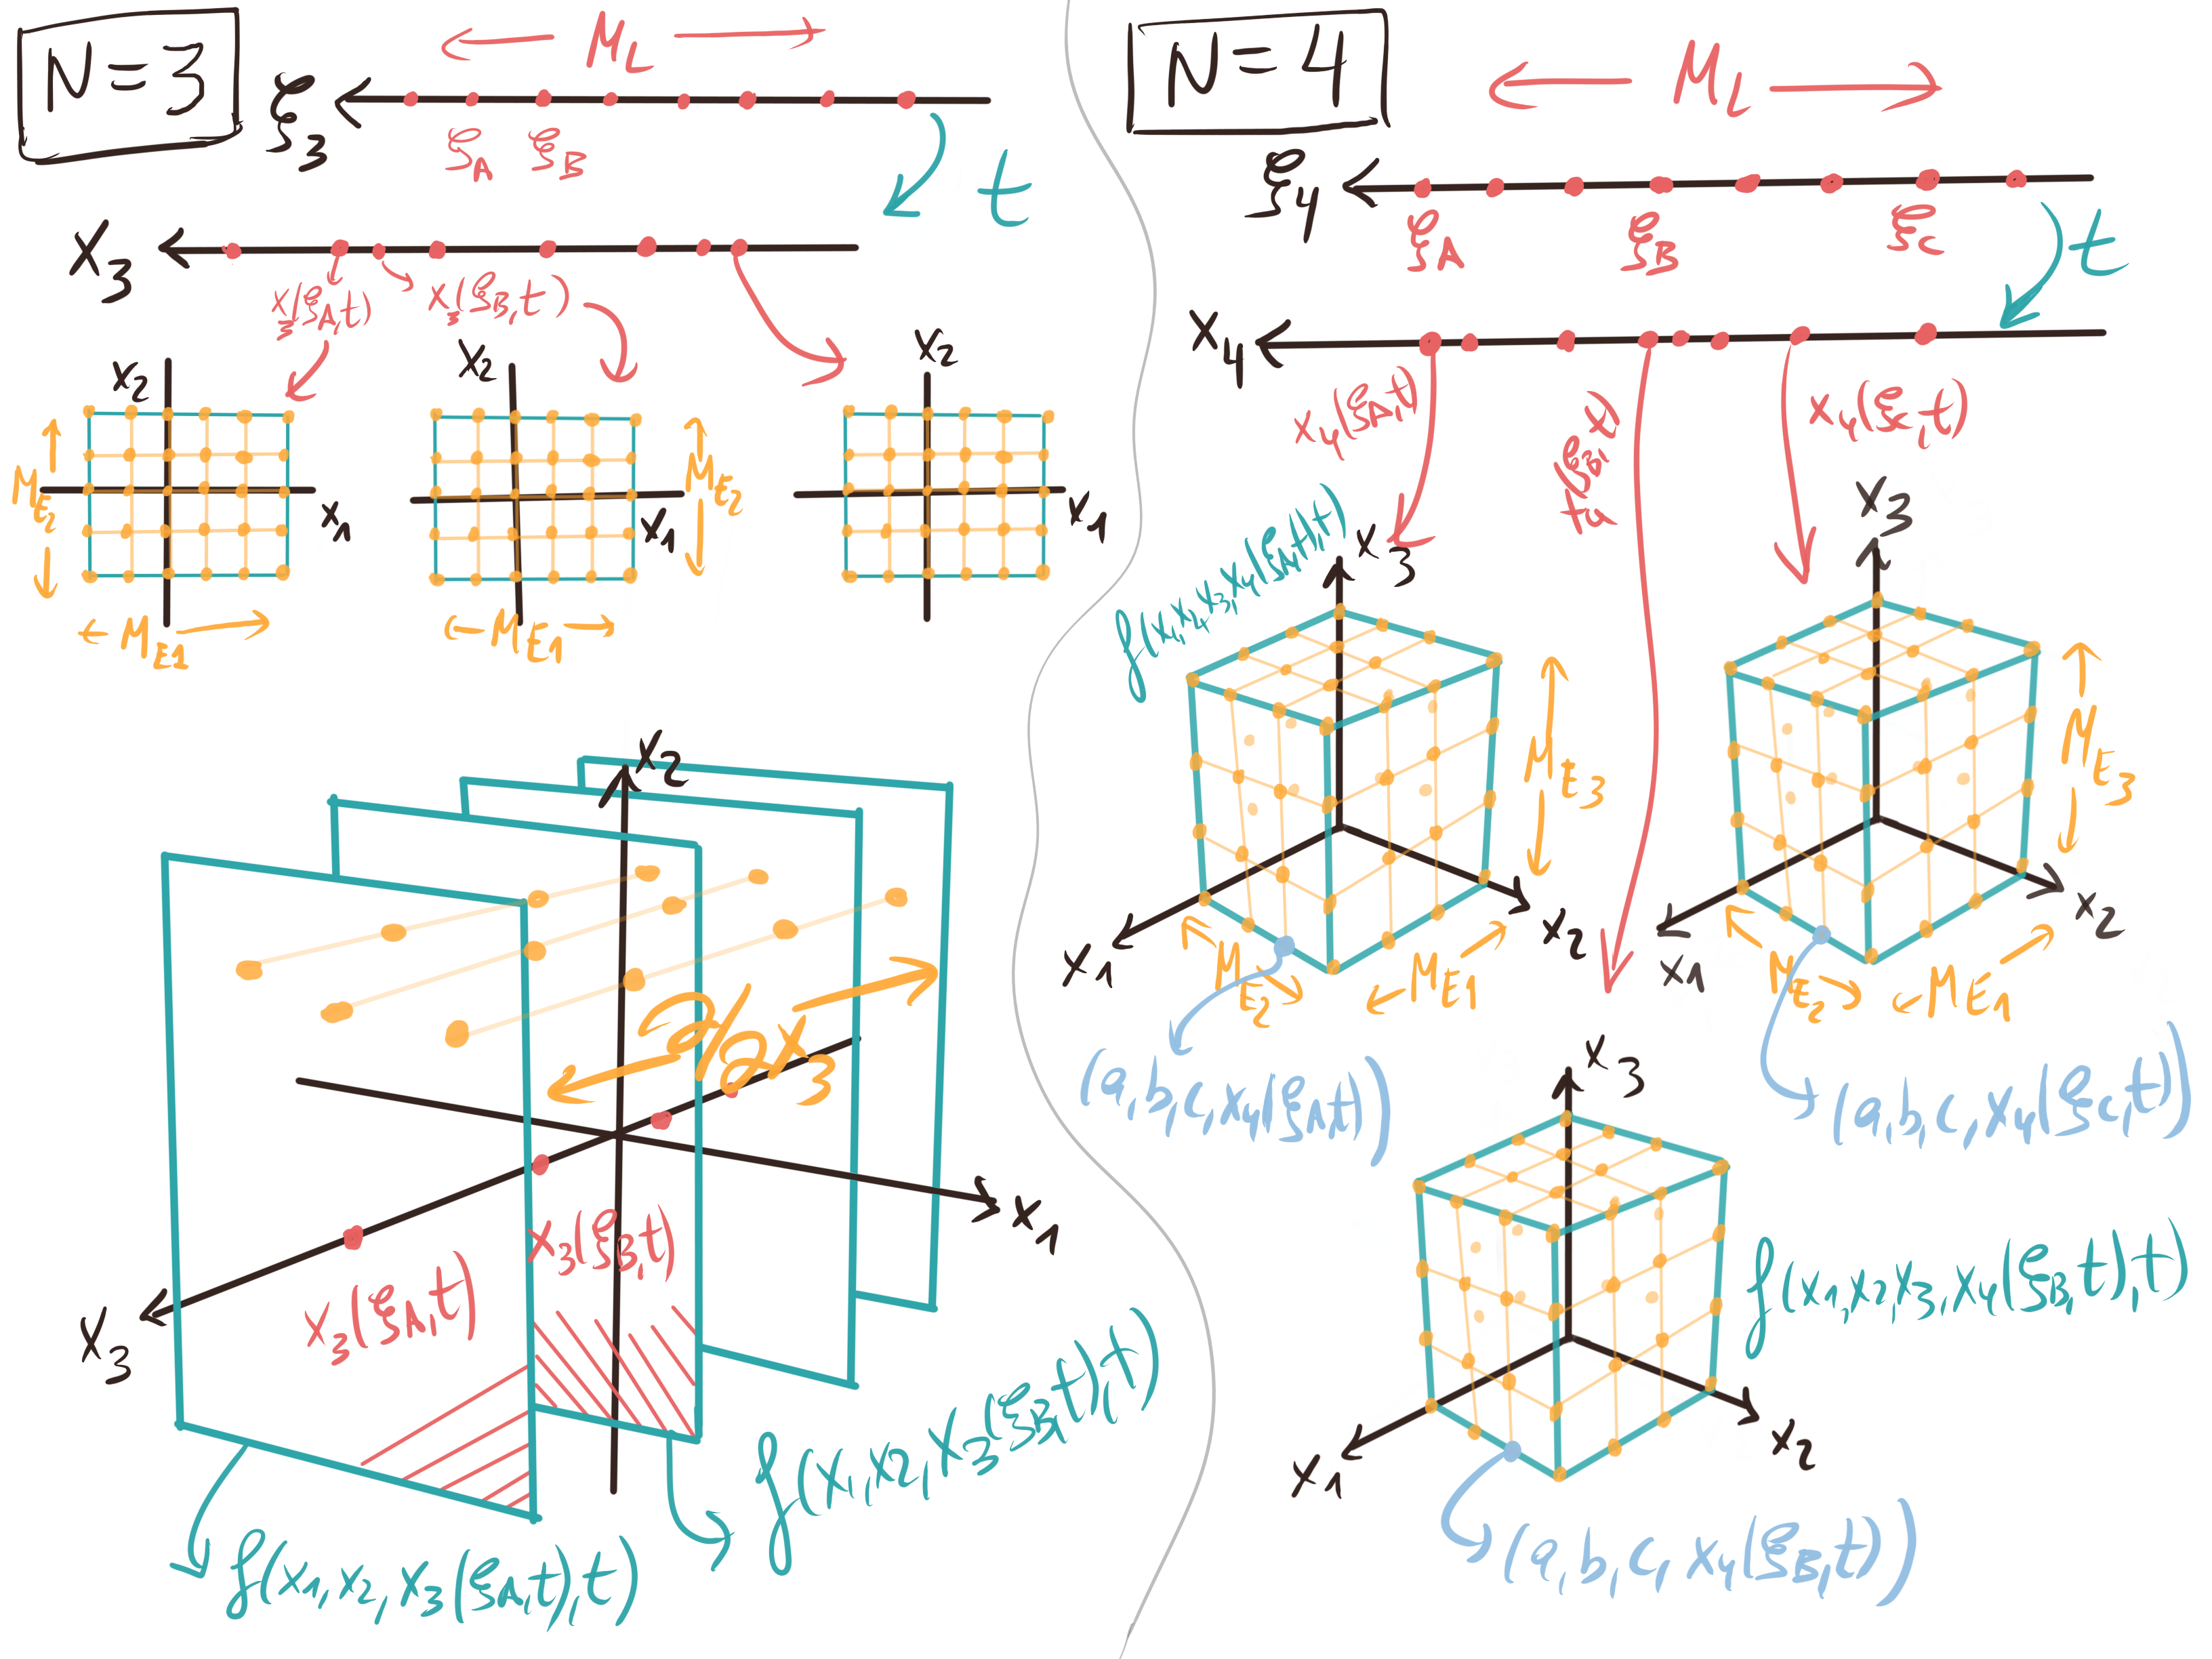
\includegraphics[width=1\linewidth]{11one_Lagrangian.png}
  \caption{{\bf In the left} we see an intuition of the $N=3$ case of the single Lagrangian degree case. Above we see two axes, representing the equidistant distribution of the Lagrangian axis points in label space, and below a time $t$ afterwards, how they are distributed in $x_3$, following their trajectory $x_3(\xi,t)$. Each of these fluid fluid elements has associated a conditional function over a plane in $x_1,x_2$, discretized in a regular Eulerian grid. All these planes have the same number of points in $x_1,x_2$, and, very importantly, at the same positions. The relevance of them being in the same positions, can be more clearly seen below, where all these planes as slices of the support of the full function $f(x_1,x_2,x_3,t)$ are stacked in parallel each in the $x_3=x_3(\xi,t)$ position. Since the Eulerian discrete points (in yellow) are in the same $x_1,x_2$ points, they are aligned across the planes, meaning that the computation of the partial derivative $\pdv{}{x_3}$ in the Lagrangian axis will be computable from plane to plane even if the distance between the planes varies due to the movement of the coupled fluid element in $x_3$. Each of these lines traversing the planes along the same Eulerian points is what in the text we call a derivative {\bf beam}. \vspace{0.3cm}\\
{\bf In the right}, we can see a depiction with the same particularities, just that we represent a $N=4$ quantum system, where the support of each conditional function is a discretized $\R^4$ hyperplane, a 3D box. It is filled with Eulerian nodes, which again have the same positions between the different trajectories to allow the derivatives in the $x_4$ (Lagrangian) axis. This is aimed to be represented by noting in blue that all the hyperplane-boxes have the same point $(a,b,c)$ just with $x_4$ equalling their trajectory position. }
  \label{fig:hyperplane}
\end{figure}

Then an algorithm to evolve the ensemble of hyperplane-conditional functions could be the following. Given we have an initial ensemble of $M$ hyperplane-conditional functions and initial trajectory positions (rather $\vec{x}(\vec{\xi},t)$ or $\vec{y}(\vec{\xi}_y,t)$ depending on our choice of underlying fluid) labelled by their underlying fluid element $\vec{\xi}^j$:
\begin{enumerate}
\item Share the information of the conditional functions in the necessary parallel processors.
\item Compute {\em in parallel} the derivatives in the Lagrangian axes for each hyperplane-conditional function $\vec{\xi}^j$. For this, access the same $(x_1,...,x_{N-1})$ point in each adjacent slice. Compute the necessary derivatives (first and/or second) to get the correlation terms. Consult the formulas.
\item Evaluate the correlation terms of the current time step for each point $(x_1,...,x_{N-1})$ in each hyperplane\footnote{Note we called them correlation terms, because they introduce the effects of the rest of possible conditional functions.}.
\item Gather the correlation terms to time evolve in parallel to the next time step each hyperplane-conditional function, using one process per $\vec{\xi}^j$. This will be done with the necessary algorithm for an $m=N-1$ dimensional function.
\item Go back to 1.
\end{enumerate}


As a little computational detail, if we choose the Lagrangian degrees to move, an initially regular grid in the $x_N$ axis (constituted by the different hyperplanes) will get unstructured. The distances between the hyperplanes will become irregular. This will make the following derivatives in the Lagrangian axis be more difficult to compute. We could then take one of these solutions to compute the derivatives:
\begin{itemize}
\item Fit an analytical function sum to each locality (each stencil of elements we will use to compute the derivatives), and get their symbolical derivative. It involves all the fitting burden.
\item Use some finite difference method in not equispaced grids (this will only work in the case of a single Lagrangian axis, since otherwise the fluid elements will not be aligned in $t>t_0$).
\item Compute the derivatives relative to the label space, which can be chosen to be regular, as explained in (III.e). It involves all the Jacobian determinant (or inverse Jacobian) computation burden.
\item We could choose to fix the trajectory $x_N^\xi(t)=\xi\ \forall t>t_0$ (since remember the equations for conditional functions do not force us to make them be Bohmian trajectories). In such a case, the derivatives would always be in a regular grid and could be computed easily with advanced finite differences. This would be a subtle way to turn back to the Eulerian fixed grid though, where the grid is stationary! It is this why we said in an Eulerian grid all this parallelization was actually possible as well, just that we needed the fluid view to realize it.
\end{itemize} 



\subsection*{N-m Lagrangian degrees}
In order to generalize the algorithm, we will use as an example the 2 Lagrangian degree case, which will provide us with a visual intuition, allowing us to find a pattern and induce the generalization. You can find a visual understanding of the 2 Lagrangian degree case in Figure \ref{fig:hyperplane2}.

\begin{figure}[p!]
  \centering
    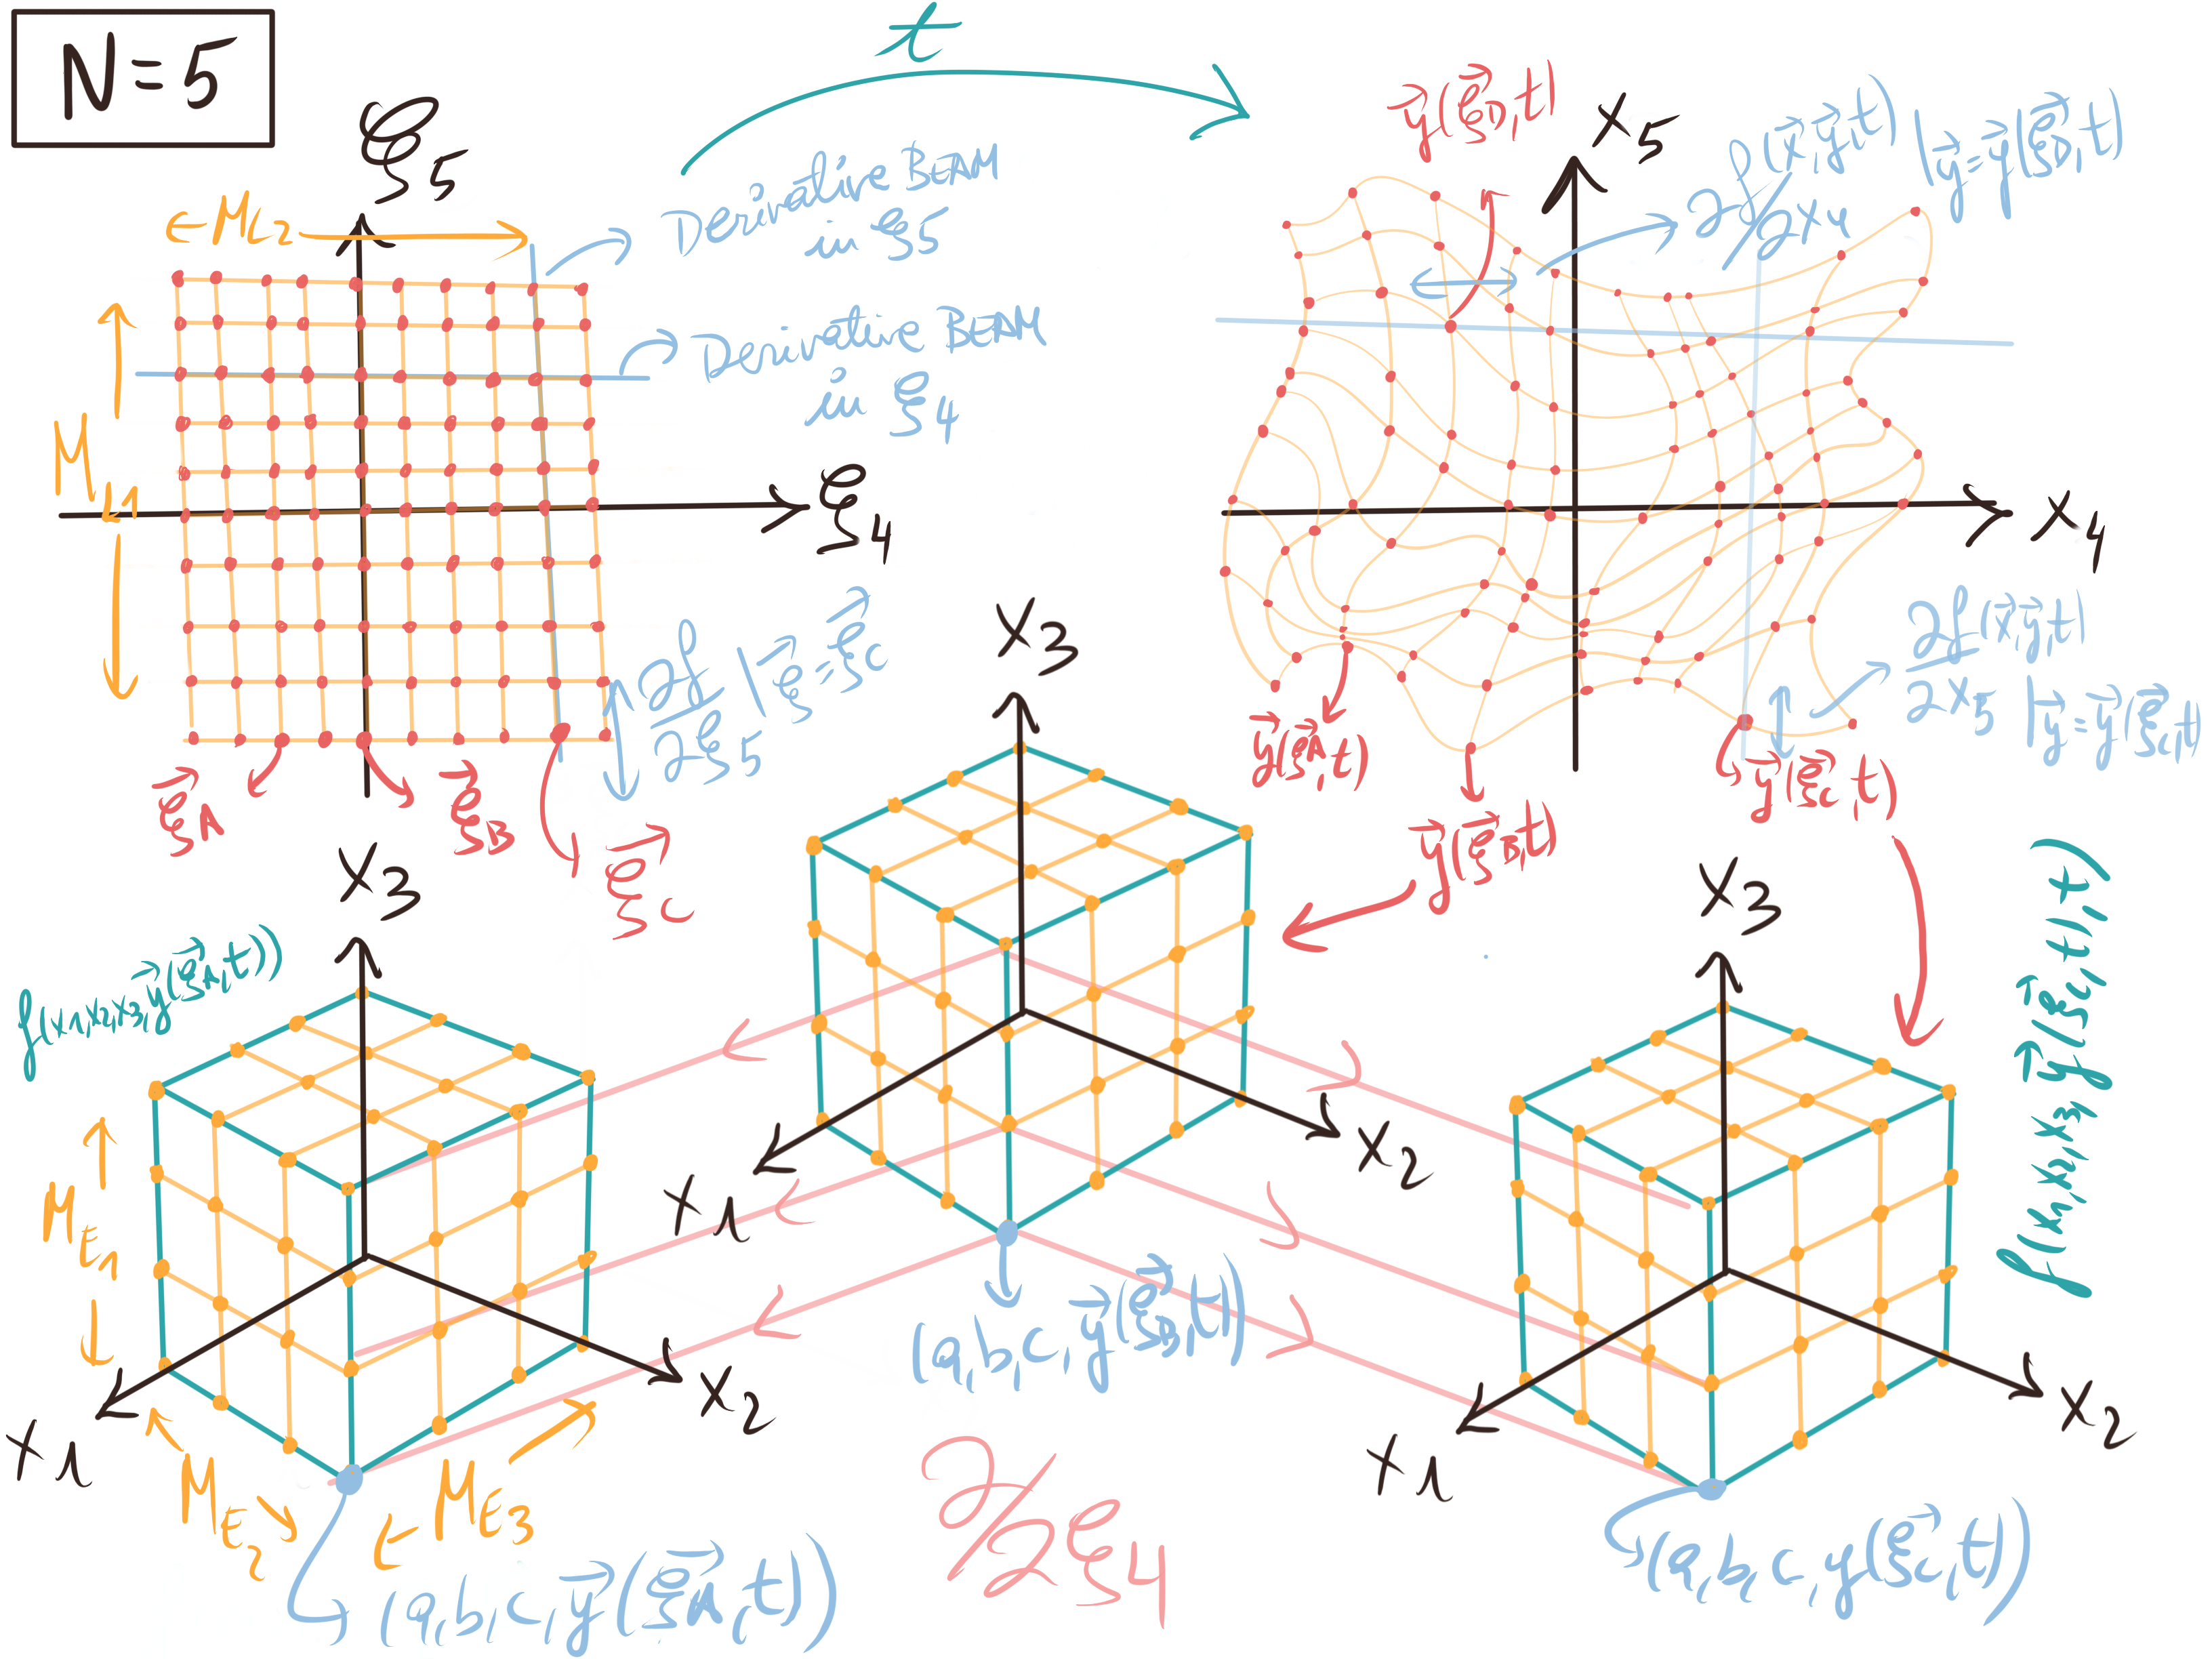
\includegraphics[width=1\linewidth]{12_N6.png}
  \caption{This is a visual intuition of a quantum system with $N=5$, where there are two Lagrangian degrees. Above left we see two axes, representing the equidistant distribution of the Lagrangian axis points in label space, and above right, a time $t$ afterwards, how they are distributed in the $x_4,x_5$ plane, following their trajectories $\vec{y}(\vec{\xi},t)=(x_4(\vec{\xi},t),x_5(\vec{\xi},t))$. Each of these fluid elements has associated a conditional function over a 3D space in $x_1,x_2,x_3$, discretized in a regular Eulerian grid as a box. All these Eulerian boxes have the same number of points in $x_1,x_2,x_3$, and, very importantly, at the same positions, which is represented in blue as saying that all of them have the corner $\vec{x}=(a,b,c)$ with $\vec{y}=\vec{y}(\vec{\xi},t)$. The relevance of them being in the same positions is that when we move from a conditional function to the next (to the one aligned in the Lagrangian space with the first), to compute Lagrangian space derivatives we will need to take care for the same Eulerian point within each box. These same points in each conditional function define what we called a derivative {\bf beam} (depicted in pink lines with arrows joining the boxes). The beam's description is completed by selecting a line joining these conditional functions in Lagrangian axis space. This last thing is depicted in blue in the planes above. We can see that in the label space, any derivative beam contains many representatives, but when the grid gets distorted the beams only catch some few conditional functions aligned. That is, the grid for derivatives gets unstructured. It is this why it is way more convenient if we simply change the derivatives in configuration space to derivatives in label space. The beams in label space are full of representatives for numerical derivative computations.  }
  \label{fig:hyperplane2}
\end{figure}


The algorithm would be left almost the same: given we have an initial ensemble of $M_L^{N-m}$ conditional functions\footnote{We will choose to have as many conditional functions as the necessary ones to have a representative per point in an initial regular grid in the whole Lagrangian axis subspace. We will have $M_L$ points in each axis, meaning we will consider a total of $M_L^{N-m}$ Lagrangian fluid elements and their conditional functions.} and initial trajectory positions (rather $\vec{x}(\vec{\xi},t)$ or $\vec{y}(\vec{\xi}_y,t)$ depending on our choice of underlying fluid), each labelled by their underlying fluid element $\vec{\xi}^j$:
\begin{enumerate}
\item Share the information of the conditional functions in the necessary parallel processors.
\item Compute {\em in parallel} the derivatives in the Lagrangian axes for each conditional function $\vec{\xi}^j$. In this case, this is a bit more subtle, since we have problematic partial derivatives in the $N-m$ different Lagrangian directions. We need for each possible point in the $m$ dimensional support of each conditional function, each $(x_1,...,x_{m})$ point of each slice, the variation of the function between the conditional functions whose Lagrangian degrees are aligned in the Lagrangian direction. There are $N-m$ Lagrangian directions, and we need the derivative in all of them. Then, compute the necessary derivatives (first and/or second) to get the correlation terms.
\item Evaluate the correlation terms of the current time step for each point $(x_1,...,x_{m})$ in each $m$ dimensional affine manifold (each conditional function).

\item Gather the correlation terms to time evolve in parallel to the next time step each conditional function, using one process per $\vec{\xi}^j$. This will be done with the necessary algorithm for an $m$ dimensional conditional function.
\item Go back to 1.
\end{enumerate}


The derivatives this time will be required to be computed in a grid where not only the distance between the conditional functions in the Lagrangian degrees will get irregular, but where also, the alignment in the Lagrangian directions for the conditional functions will be distorted (as can be understood in the Figure \ref{fig:hyperplane2}). That is, we will have a totally unstructured mesh. To solve these derivatives:
\begin{itemize}
\item Fit an analytical function sum to each locality (each stencil of elements we will use to compute the derivatives), and get their symbolical derivative. It involves all the fitting burden.
\item Compute the derivatives relative to the label space, which can be chosen to be regular, as explained in (III.e). It involves all the Jacobian determinant (or inverse Jacobian) computation burden.
\item We could chose to fix the trajectories $\vec{y}(\vec{\xi}_x, \vec{\xi}_y,t)=\vec{\xi}_y\ \forall t>t_0$. In such a case, the derivatives would always be in a regular grid and could be computed easily with finite differences. This would be a subtle way to turn back to the Eulerian fixed grid though, where the grid is stationary! It is this why we said in an Eulerian grid all this parallelization was actually possible as well, just that we needed the fluid view to realize it.
\end{itemize}

In order to have an idea of the complexity of a possible algorithm following these steps, we we will exemplify it with the $G$ and $J$ correlation potential method \eqref{SE.GJ}, where to compute the derivatives, we will use the conversion to label space derivatives (it would be way simpler if we just left the trajectories still, but this way we will get a bigger picture).

Consider as we said, that we take $M_L^{N-m}$ trajectories, such that they discretize each Lagrangian axis in $M_{L}$ different discrete points, making an equidistant regular mesh of the $\vec{y}$ subspace. Then, consider we discretize each conditional function of $m$ Eulerian dimensions in $M_E^m$ points in $\R^m$, also as a regular and equispaced mesh with $M_E$ points per axis.

Lets now follow the algorithm step by step manifesting a possible complexity of each step if we allow an arbitrary number of parallel processes. The movement of data and the management of the processes will not be efficient at all, it is instead just intended to be illustrative:
\begin{enumerate}
\item Have all the $M_L^{N-m}$ conditional wavefunctions distributed each in $M_L^{N-m}$ parallel processors.
\item Make each processor compute the conditional action and C amplitudes of each wavefunction, for which each will require in parallel $O(M_E^m)$ operations, since they will require to consult each point of the conditional wavefunction $O(1)$ times.
\item In order to compute the potentials $G$ and $J$ of each one of the $M_L^{N-m}$ conditional functions, we need to compute 4 different derivatives ($\pdv{S}{x_k}$, $\pdv[2]{S}{x_k}$, $\pdv{C}{x_k}$, $\pdv[2]{C}{x_k}$) per Lagrangian axis $k\in\{m+1,...,N\}$. A total of $4(N-m)$ derivatives of the conditional functions in the Lagrangian axes are required. Since we will change them to the label space using $\pdv{f(\vec{x}, \vec{y},t)}{x_k}\Big\rvert_{\vec{y}(\vec{\xi},t)}=\sum_{j=m+1}^N \pdv{f(\vec{x},\vec{y}(\vec{\xi},t),t)}{\xi_j} \pdv{\xi_j(\vec{x},t)}{x_k}\Big\rvert_{\vec{x}(\vec{\xi},t)}$, we will only compute the $\pdv{f}{\xi_k}$ once, then we will share them for the computation of all the Lagrangian axis $x_k$ derivatives. For the second derivatives we will compute the derivatives of the first derivatives sequentially. We have the following tasks then:
\begin{enumerate}
\item Compute for $f\in\{S,C\}$ the $N-m$ derivatives $\pdv{f(\vec{x},\vec{y}(\vec{\xi}_y,t),t)}{\xi_j}$. For this, notice that if we fix all the variables except for one $\xi_j$, this defines a line in $\R^N$ where we have all the necessary function values to compute the derivative $\pdv{}{\xi_j}$ in each value of $\xi_j$. Let us call this line a partial derivative {\bf beam}. Then, for each value of the rest of labels and each Eulerian position $\vec{x}$, we have a different beam of these. For an intuition look at the Figures \ref{fig:hyperplane} and \ref{fig:hyperplane2}. In total we have $M_L^{N-m}M_E^m$ beams like this one for each of the $(N-m)$ directions $\vec{\xi_j}$ in label space. Each beam contains all the information to compute the derivatives in a regular equispaced grid, for any point along the beam (each point in the beam belongs to a different conditional function). If we use for example a five point finite difference method, this can be done by running over each beam of $M_L$ elements five times, which means $O(5M_L)$ operations. Thus, we could have in parallel $O(2(N-m)M_L^{N-m-1}M_E^m)$ processes each computing $O(5M_L)$ operations. Then in $O(5M_L)$ linear time, all the derivatives $\pdv{f}{\xi_k}$ at all points would be computed for $f\in\{S,C\}$. Of course, to begin with this, each process that in (1) had its conditional function would need to send all the elements to each processor that will take care for each beam. Since each conditional function point is part of $N-m$ beams, $2(N-m)M_E^m$ messages would be required to be sent, taking $O(2\theta (N-m)M_E^m)$ time, where $\theta$ is the average time for each number delivery.\\

\item The derivatives $\pdv{\xi_j(\vec{x},t)}{x_k}$ would also be required to be computed. To do this, we saw in (II.e) that we could first compute the Jacobian matrix, composed of derivatives $\pdv{\x_k(\vec{\xi},t)}{\xi_j}$ in label space for the trajectories, and then invert the matrix. In order to compute these derivatives, we can do the same strategy as before (just that now we will only have a single representative in each Lagrangian position). There are a total of $O(M^{N-m})$ beams per Lagrangian $\xi_k$, a total of $O((N-m)M_L^{N-m})$. Since they are $N$ trajectory positions as much, we could make one every $M_E^m$ processes of the previous step take $N$ of these beams. Each would compute the derivatives in $O(5NM_L)$ operations. Each process that had the conditional functions has its own trajectory value (composed by maximum $N$ numbers), each has to be shared with $N-m$ processes, meaning a messaging time of $O(N\theta (N-m))$.\\

\item Once $(a)$ and $(b)$ are done, each process that in $(1)$ had a complete conditional function, receives the derivatives $\pdv{S}{\xi_k}$ and $\pdv{C}{\xi_k}$ at their Lagrangian position $\vec{\xi}^j$ together with each of their $M_E^m$ Eulerian positions $\vec{x}$ from processes that worked in $(a)$. Then they also receive a maximum of $N$ values of $\pdv{\vec{x}}{\xi_k}$ for their trajectory. To receive all of this, they will require again $O(4\theta (N-m)M_E^m+N\theta (N-m))$ message reception time (the senders only need to send asynchronously $(N+4)M_L$ messages, which is less time than the reception time).\\

\item Each of these $M_L^{N-m}$ processes has now an entire conditional wavefunction and the derivatives of the conditional action and C amplitude in label space along their trajectory position. They also have the derivative of their trajectory diffeomorphism along their trajectory position, which are a maximum of $N\times N$ numbers. They could now compute the inverse Jacobain matrix at their trajectory's position in $O(N^3)$ operations using the well known Gauss-Jordan Elimination algorithm. This inverse, would grant them, the values of $\pdv{\xi_j}{x_k}$ in their trajectory position. With this, they would be able to compute $\pdv{f}{x_k}$ in their trajectory position for $f\in\{S,C\}$ for all the Lagrangian $x_k$. To do this, they would require a maximum of $N$ products and $N$ sums per conditional function point. A total of $O(2NM_E^m)$ operations.\\

\item The whole (a) to (d) would be repeated to compute the second derivatives.
\end{enumerate}
This would leave the computation of the derivatives in the Lagrangian spatial axes in a total of:
$$
\hspace{-0.9cm}O\qty(2\qty[6\theta(N-m)M_E^m+5M_L+5NM_L+2N\theta(N-m) +2NM_E^m])=
$$
$$
=O\qty(M_E^m(N(\theta+1)+\theta m)+N(M_L+\theta(m+N)))
$$

\item Then each process that has a whole conditional function and the computed derivatives for its trajectory would be able to obtain the correlation potentials $G$ and $J$ for its Eulerian positions. These are ten products and four sums times $(N-m)$ per Eulerian position. A total of $O(14(N-m)M_E^m)$ operations.
\item Finally, each of these $M_L^{N-m}$ processes would only need to evolve one time step of their conditional wavefunctions using the computed correlation potentials. Using a Crank Nicolson algorithm, this would take $O(M_E^m)$ operations. They would then get the conditional wavefunction at the next time step. With it, they could evolve their trajectories as well in $O(1)$ operations.
\end{enumerate}
If we consider that in reality, it was not just a conditional wavefunction per trajectory but a set of about $N/m$ complementary conditional wavefunctions (for instance, to allow the evolution of a Bohmian trajectory with no further interpolation), we would just need to multiply all the computational time by $N/m$ and assume wherever we said there was a conditional wavefunction, that there were all its complementary ones.

Even in this case, the total linear time that all the process would take is:
\begin{equation}
T_{N,m}:=O\qty(N\qty(M_E^m(N(\theta+1)+\theta m)+N(M_L+\theta(m+N))+M_E^m+14(N-m)M_E^m+N^3))=
\end{equation}
$$
=O\qty(NM_E^m\qty[1+N(\theta+1)+m(\theta+1)]+N^2\qty[N^2+M_L+\theta(m+N) ])
$$
For this, the number of parallel processes we have used is $O((N-m)M_L^{N-m}M_E^{m})$, which if $M_L=M_E=M$ means $O((N-m)M^{N})$ processes.

In a nutshell, we will require exponentially more parallel processes $O((N-m)M^{N})$ to simulate quantum systems with more dimensions $N$. In exchange, in terms of linear time, the simulation will only take a polynomial time more, since $T_{N,m}$ only increases as $O(N^4)$ for a fixed number of Eulerian degrees $m$ (and leaving the rest of parameters fixed as well).

Actually, by looking at these results, we clearly see that as we increase the relative number of Lagrangian degrees of freedom (we reduce $m$), we will require linearly more parallel processes, but the effective sequential computation time will be reduced exponentially. In the limit of $m=0$, we will have the minimum effective computational time. This would be the case of the fully Lagrangian picture. Conversely, as we increase the relative number of Eulerian degrees of freedom (increase $m$), we see that the computational time will increase exponentially and we will need less parallel processes. In the limit of the fully Eulerian Schrödinger Equation with no fluid treatment, we would have that its computation time is exponential with dimensions $O(M_E^N)$, but we will have enough with a single process.

An easier algorithm would be to consider the trajectories are stationary. This would make the Lagrangian grid regular at all times, making the derivatives computable with finite differences, without the need for the Jacobian matrix endeavour. The conclusions would be even clearer in that case.



%\begin{figure}[h!]
%  \centering
%    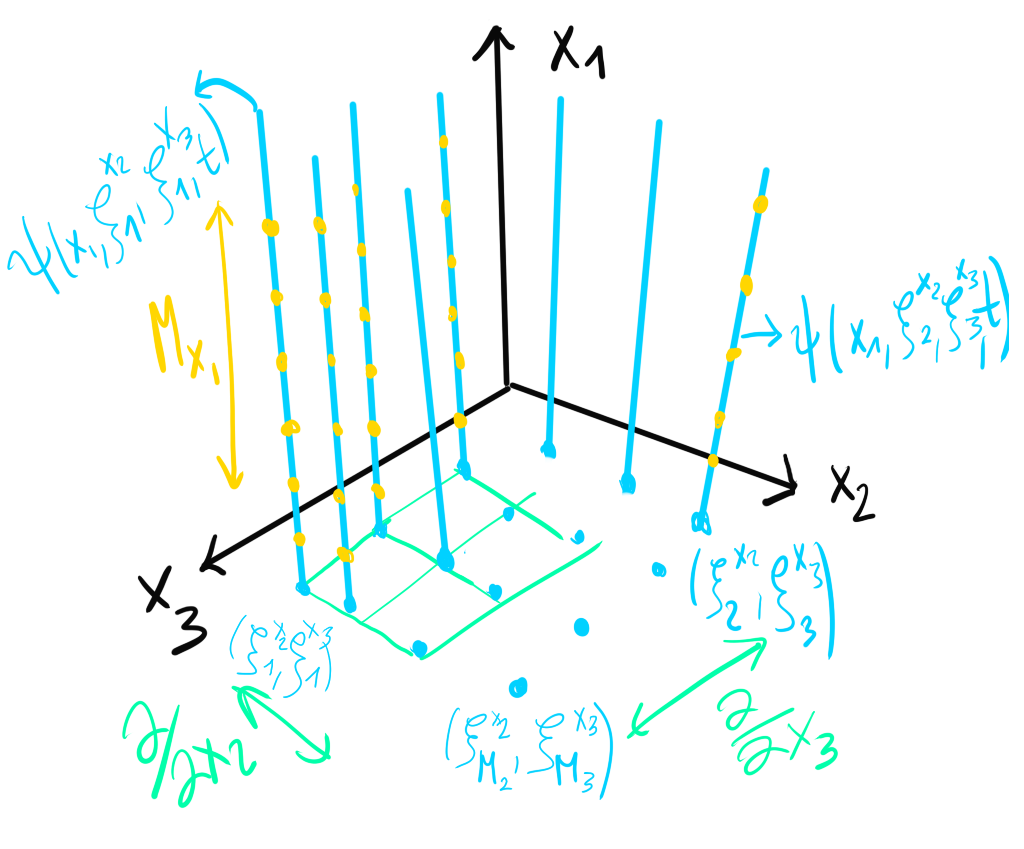
\includegraphics[width=0.5\linewidth]{rectas.png}
%  \caption{In blue, the $M_{x2}xM_{x3}$ CWF-s, the supports of which are 1D manifolds. In yellow, the $M_{x1}$ discrete points we consider in each CWF. Note how the yellow points in $x_2$ and $x_3$ are aligned in a regular grid, meaning they can be used to compute numerically the derivatives in the Lagrangian directions.  }
 % \label{fig:lines}
%\end{figure}




\newpage
\subsection*{What could the advantage of the Part Lagrangian Part Eulerian approach be?}
Apart from theoretical considerations, we might be able to get the best of both worlds at once: the Eulerian and the Lagrangian. It must be noted however that we would also get the worst of both worlds at once. We would still need matrix methods like in the Eulerian frame and at the same time we would need, just like in the Lagrangian frame, function fitting, Jacobian matrices and determinants or infinite equation chains.

Among the relevant positive points, here are some of the most interesting ones:

\begin{itemize}
\item We have simple control over the parallelization-sequential computation tread-off:

\begin{itemize}
\item The more Eulerian degrees we consider, the smaller the space for sampling the trajectories of the Lagrangian part will be. This means that the less conditional functions will be required to reproduce the full functions or to achieve a certain precision in the derivatives in Lagrangian directions. However, the more computationally complex will be the conditional functions to evolve, so the problem gets more complex to be parallelized. In the limit, of $m=N$ we would recover the linear Schrödinger equation in the Eulerian frame, which typically scales exponentially in time with dimensions.

\item The more Lagrangian degrees we consider, the more trajectories we will need to reconstruct the full functions and to get the derivatives in the Lagrangian directions. Exponentially more in fact, since the net Lagrangian space will be a product of subspaces. However, the conditional functions will be simpler to evolve and as the trajectories can (and must) be computed coupled but in parallel, the more of exponential complexity we will transfer to parallel threads. In the limit of $m=0$, we recover the fully Lagrangian frame, where we conceptually achieve the apparently highest parallelizability of the Quantum many body problem.
\end{itemize} 



\item Unlike the fully Lagrangian frame, for $m\neq 0$, each trajectory will be accompanied by lots of full function points (proportionally more with the amount of Eulerian degrees). Interpolating the full function or knowing information about it would therefore be simpler. For instance, a nearest neighbour approach would be more accurate in the reconstruction task.

\item The grid is preserved in a structured manner at all times for the Eulerian degrees, while it gets unstructured for the Lagrangian axes. If complementary conditional functions are present, there are parts of the Lagrangian axes for one conditional function that are Eulerian for the other, so there is always track of the function in all the extent of the simulation domain in variable precisions.
\item {\bf Fast and Slow Degrees of Freedom}: conditional functions provide a natural way to treat the slow degrees of freedom separated form the fast ones. This is the case in an atomic nucleus relative to its orbiting electrons. It is common in molecular dynamics algorithms to consider classical trajectories for slow parts of the quantum system while quantum wavefunctions for other parts. The partially Lagrangian approach (which is fully quantum) could be used to improve these methods and dress them with an {\em ab initio} look.
\item It is a perfect sandbox for performing {\em ad-hoc} {\bf approximations} to different degrees of freedom in different ways, allowing us to select a subsystem $m$ of interest and treat it as if it really had $m$ dimensions, without the need to directly neglect the environment. The correlation terms separately show the effects and interactions with each Lagrangian degree axis, so we could apply different approximations or different {\em a priori} knowledge about the correlations as a function of the Lagrangian degree.
\end{itemize}




% d) Hybrid approaches, escenarioko zati bet dynamikoki bihurtu finaue edo beste approach batera. Problemas? MBP ezu supereko eta fronterien tratamentue klaro ejem. Ta bai eboluziñoa establiaue izengo da for sure, however, comput complexity ++ kambixo bakoitzeko problema kalro!



\newpage
\section*{IV . No Continuous Wave, just Discrete Trajectories}
\addcontentsline{toc}{subsection}{\bf IV . No Continuous Wave, just Discrete Trajectories}

Writing in progress...

Meanwhile, note that there seems to be a research line that has already worked on this! One of the first papers on this line seems to be:

Hall, M. J., Deckert, D. A., \& Wiseman, H. M. (2014). {\em Quantum phenomena modeled by interactions between many classical worlds.} Physical Review X, 4(4), 041013.



 
\fancyhead[L]{\em References}


\begin{thebibliography}{1}
\addcontentsline{toc}{section}{References}

\bibitem{JordiXO}
	Oriols X, Mompart J, {\em Applied Bohmian Mechanics: From Nanoscale Systems to Cosmology} Pan Stanford, Singapore (2012)
	
%\bibitem{XO}
%	Oriols X. 2007 {\em Quantum-trajectory approach to time-dependent transport in mesoscopic systems with electron-electron interactions} Phys. Rev. Lett. 98 066803

\bibitem{Wyatt}
Wyatt R. E., {\em Quantum Dynamics with Trajectories} (Springer, Berlin, 2006)

%\bibitem{Dev}
%	Devashish Pandey, Xavier Oriols, and Guillermo Albareda. {\em Effective 1D Time-Dependent Schrödinger Equations for 3D Geometrically Correlated Systems.} Materials 13.13 (2020): 3033.

\bibitem{movingGrids}
Knupp, P. \& Steinberg, S.. {\em The Fundamentals of Grid Generation.} (1993) \href{https://www.researchgate.net/publication/265361548_The_Fundamentals_of_Grid_Generation}{https://www.researchgate.net/publication/265361548\_The\_Fundamentals\_of\_Grid\_Generation} 

\bibitem{Norsen}
Norsen, T., Marian, D. \& Oriols, X. {\em Can the wave function in configuration space be replaced by single-particle wave functions in physical space?.} Synthese 192, 3125–3151 (2015). \href{https://doi.org/10.1007/s11229-014-0577-0}{https://doi.org/10.1007/s11229-014-0577-0}


\bibitem{conditional1}
Norsen T., {\em Bohmian Conditional Wave Functions (and the status of the quantum state)}, 2016 J. Phys.: Conf. Ser. 701 012003

\bibitem{conditional2}
	Oriols X. 2007 {\em Quantum-trajectory approach to time-dependent transport in mesoscopic systems with electron-electron interactions} Phys. Rev. Lett. 98 066803
	
\bibitem{nireTFGie}
	Oyanguren X., {\em The Quantum Many Body Problem}, Bachelor's Thesis (2020) for the Nanoscience and Nanotechnology Degree (UAB).
\href{https://github.com/Oiangu9/The\_Quantum\_Many\_Body\_Problem\_-Bachellors\_Thesis-/blob/master/TheQuantumManyBodyProblem\_\_BachelorsThesis\_XabierOyangurenAsua.pdf}{https://github.com/Oiangu9/The\_Quantum\_Many\_Body\_Problem\_-Bachellors\_Thesis-/blob/master/TheQuantumManyBodyProblem\_\_BachelorsThesis\_XabierOyangurenAsua.pdf}


%\bibitem{conditional2}
%Albareda, G., Lively, K., Sato, S. A., Kelly, A., \& Rubio, A. (2021). {\em Conditional wavefunction theory: a unified treatment of molecular structure and nonadiabatic dynamics.} arXiv preprint arXiv: 2107.01094.


%\bibitem{Albareda}
%	Albareda G, Kelly A, Rubio A. {\em Nonadiabatic quantum dynamics without potential energy surfaces.} Phys Rev Materials. 2019; 3: 023803. 

%\bibitem{DATA}
%	All the animations employed for the analysis of Section 3.2 can be found in the following link:\\
%	\href{https://drive.google.com/drive/folders/1vnNDZrIYDlAhd-kVmmnVJgXmcdE2gxAV?usp=sharing}{https://drive.google.com/drive/folders/1vnNDZrIYDlAhd-kVmmnVJgXmcdE2gxAV?usp=sharing}
	
\end{thebibliography}


\end{document}
